\documentclass[a4paper,11pt]{book}

\usepackage[a4paper,inner=25mm,outer=44mm,top=25mm,bottom=25mm,%
            marginparsep=6mm,marginparwidth=30mm]{geometry}
\usepackage[pdftex]{graphicx} %per poter inserire le figure
\usepackage{tikz}
\usetikzlibrary{trees,arrows}
\usepackage{amssymb,amsmath,amsthm,amsfonts} % per ma matematica
\usepackage{tabularx} % per le tabelle
\usepackage{xcolor} % per i colori
\usepackage{eucal} % mathcal variant
\usepackage{url} % per gli url
\usepackage{booktabs} % per migliorare il design delle tabelle
\usepackage{listings}
\usepackage{hyperref}
\usepackage{textcomp} % for symbols
%\usepackage{cite}
\usepackage{multirow}
\usepackage[utf8]{inputenc}   %per riuscire a scrivere gli accenti
\usepackage[english]{babel}   %per riuscire a scrivere gli accenti
\usepackage{fancyhdr} %necessary to set your own header and footer style
\usepackage{comment}
\usepackage{subfiles}

%\usepackage{setspace}
%\usepackage[Bjornstrup]{fncychap}
\usepackage[labelfont=sf,textfont=normalfont,font=small]{caption}
\captionsetup{width=0.7\textwidth}

\usepackage[hyperref,backref]{biblatex}
\usepackage[babel]{csquotes}
\bibliography{Biblio}
\usepackage[symbol=$\wedge$,numberlinked=false]{footnotebackref}

\newtheorem{theorem}{Theorem}[section]
\newtheorem{corollary}{Corollary}[theorem]
\newtheorem{lemma}[theorem]{Lemma}
\newtheorem{definition}{Definition}[section]
\newtheorem{proposition}{Proposition}[section]
\theoremstyle{definition}
\newtheorem{remark}{Remark}[section]
\newtheorem{assumption}{Assumption}[section]
%\newtheorem{example}{Example}[section]
\usepackage[most]{tcolorbox}
\newtcbtheorem[number within=section]{example}{Example}%
{ % frame stuff
    breakable,
    enhanced,
    %frame empty,
    %interior empty,
    colback=white,
    colframe=black,
    %borderline west={1pt}{0pt}{black},
    boxrule=0.4pt,
    left=0.2cm,
    % title stuff
    attach boxed title to top left={yshift=-2mm,xshift=-2mm},
    coltitle=black,
    fonttitle=\bfseries,
    colbacktitle=white,
    boxed title style={boxrule=.4pt}}{example}

\usepackage{physics}
\usepackage{mathtools}
\usepackage{bm}
\usepackage{eurosym}
\usepackage{nicefrac}
\usepackage{dsfont}
\usepackage{cancel}
\usepackage{enumerate}
\usepackage{aligned-overset}
\DeclareMathOperator{\low}{Low}
\DeclareMathOperator{\prob}{Prob}
\DeclareMathOperator{\ess}{ess}
\DeclareMathOperator{\Var}{Var}
\DeclareMathOperator{\Cov}{Cov}
\DeclareMathOperator{\pay}{payoff}
\DeclareMathOperator{\call}{Call}
\DeclareMathOperator{\putt}{Put}
\DeclareMathOperator{\fwd}{FWD}
\DeclareMathOperator{\num}{NUM}
\DeclareMathOperator{\fut}{futures}
\DeclareMathOperator{\forward}{forward}
\DeclareMathOperator{\uoc}{UOC}
\newcommand{\Pmeas}{\mathbb{P}}
\newcommand{\Qmeas}{\mathbb{Q}}
\newcommand{\expect}{\mathbb{E}^{\mathbb{Q}}}
\newcommand{\besqxd}{\text{BESQ}^{\delta}_x}
\DeclarePairedDelimiter\floor{\lfloor}{\rfloor}
\newcommand{\ovun}[3]{\overset{#2}{\underset{#3}{#1}}} % over and under
\newcommand{\indep}{\raisebox{0.05em}{\rotatebox[origin=c]{90}{$\models$}}}

\usepackage{marginnote}
\newcommand{\lesson}[2]{\marginnote{\footnotesize\textsl{Lesson #1 of \\ #2}}}

\newcommand{\hlc}[2]{%
  \colorbox{#1!50}{$\displaystyle#2$}}

\definecolor{mypink}{RGB}{221, 197, 209}
\definecolor{mylightblue}{RGB}{205, 218, 233}
\definecolor{mytweed}{RGB}{180, 198, 186}

\allowdisplaybreaks %allow pagebreaks in align enviroments

\author{Matteo Bortoletto}
\title{\textsc{Stochastic Methods for Finance}}

% custom chapter style
\usepackage{titlesec, color}
\definecolor{gray75}{gray}{0.75}
\newcommand{\hsp}{\hspace{20pt}}
\titleformat{\chapter}[hang]{\Huge\bfseries}{\thechapter\hsp\textcolor{gray75}{$\mid$}\hsp}{0pt}{\Huge\bfseries}

%%%%%%%%%%%%%%%%%%%%%%%%%%%%%%%%%%%%%%%%%%%%%%%%%%%%%%%%%%%%%%
%%%%%%%%%%%%%%%%%%%%%%%%%%%%%%%%%%%%%%%%%%%%%%%%%%%%%%%%%%%%%%

\begin{document}
\thispagestyle{empty}
\newgeometry{total={170mm,257mm}, left=20mm, top=20mm}
\vspace*{3cm}
\begin{center}
                \line (1,0){350} \\
                \huge{\textsc{Stochastic Methods for Finance}}\\
                [2mm]
                \textsc{\normalsize Prof. Martino Grasselli}
                \vspace{-0.5em}\\
                \textsc{\normalsize University of Padova}\\
                \vspace{-0.7em}
                \line (1,0){350} \\
        [0.2cm]
        \textsc{\normalsize Written by: Matteo Bortoletto}\\
                \textsc{\normalsize Academic Year 2019/20}\\
        {\scriptsize Compiled on \today}\\
        \vspace*{1.5cm}
        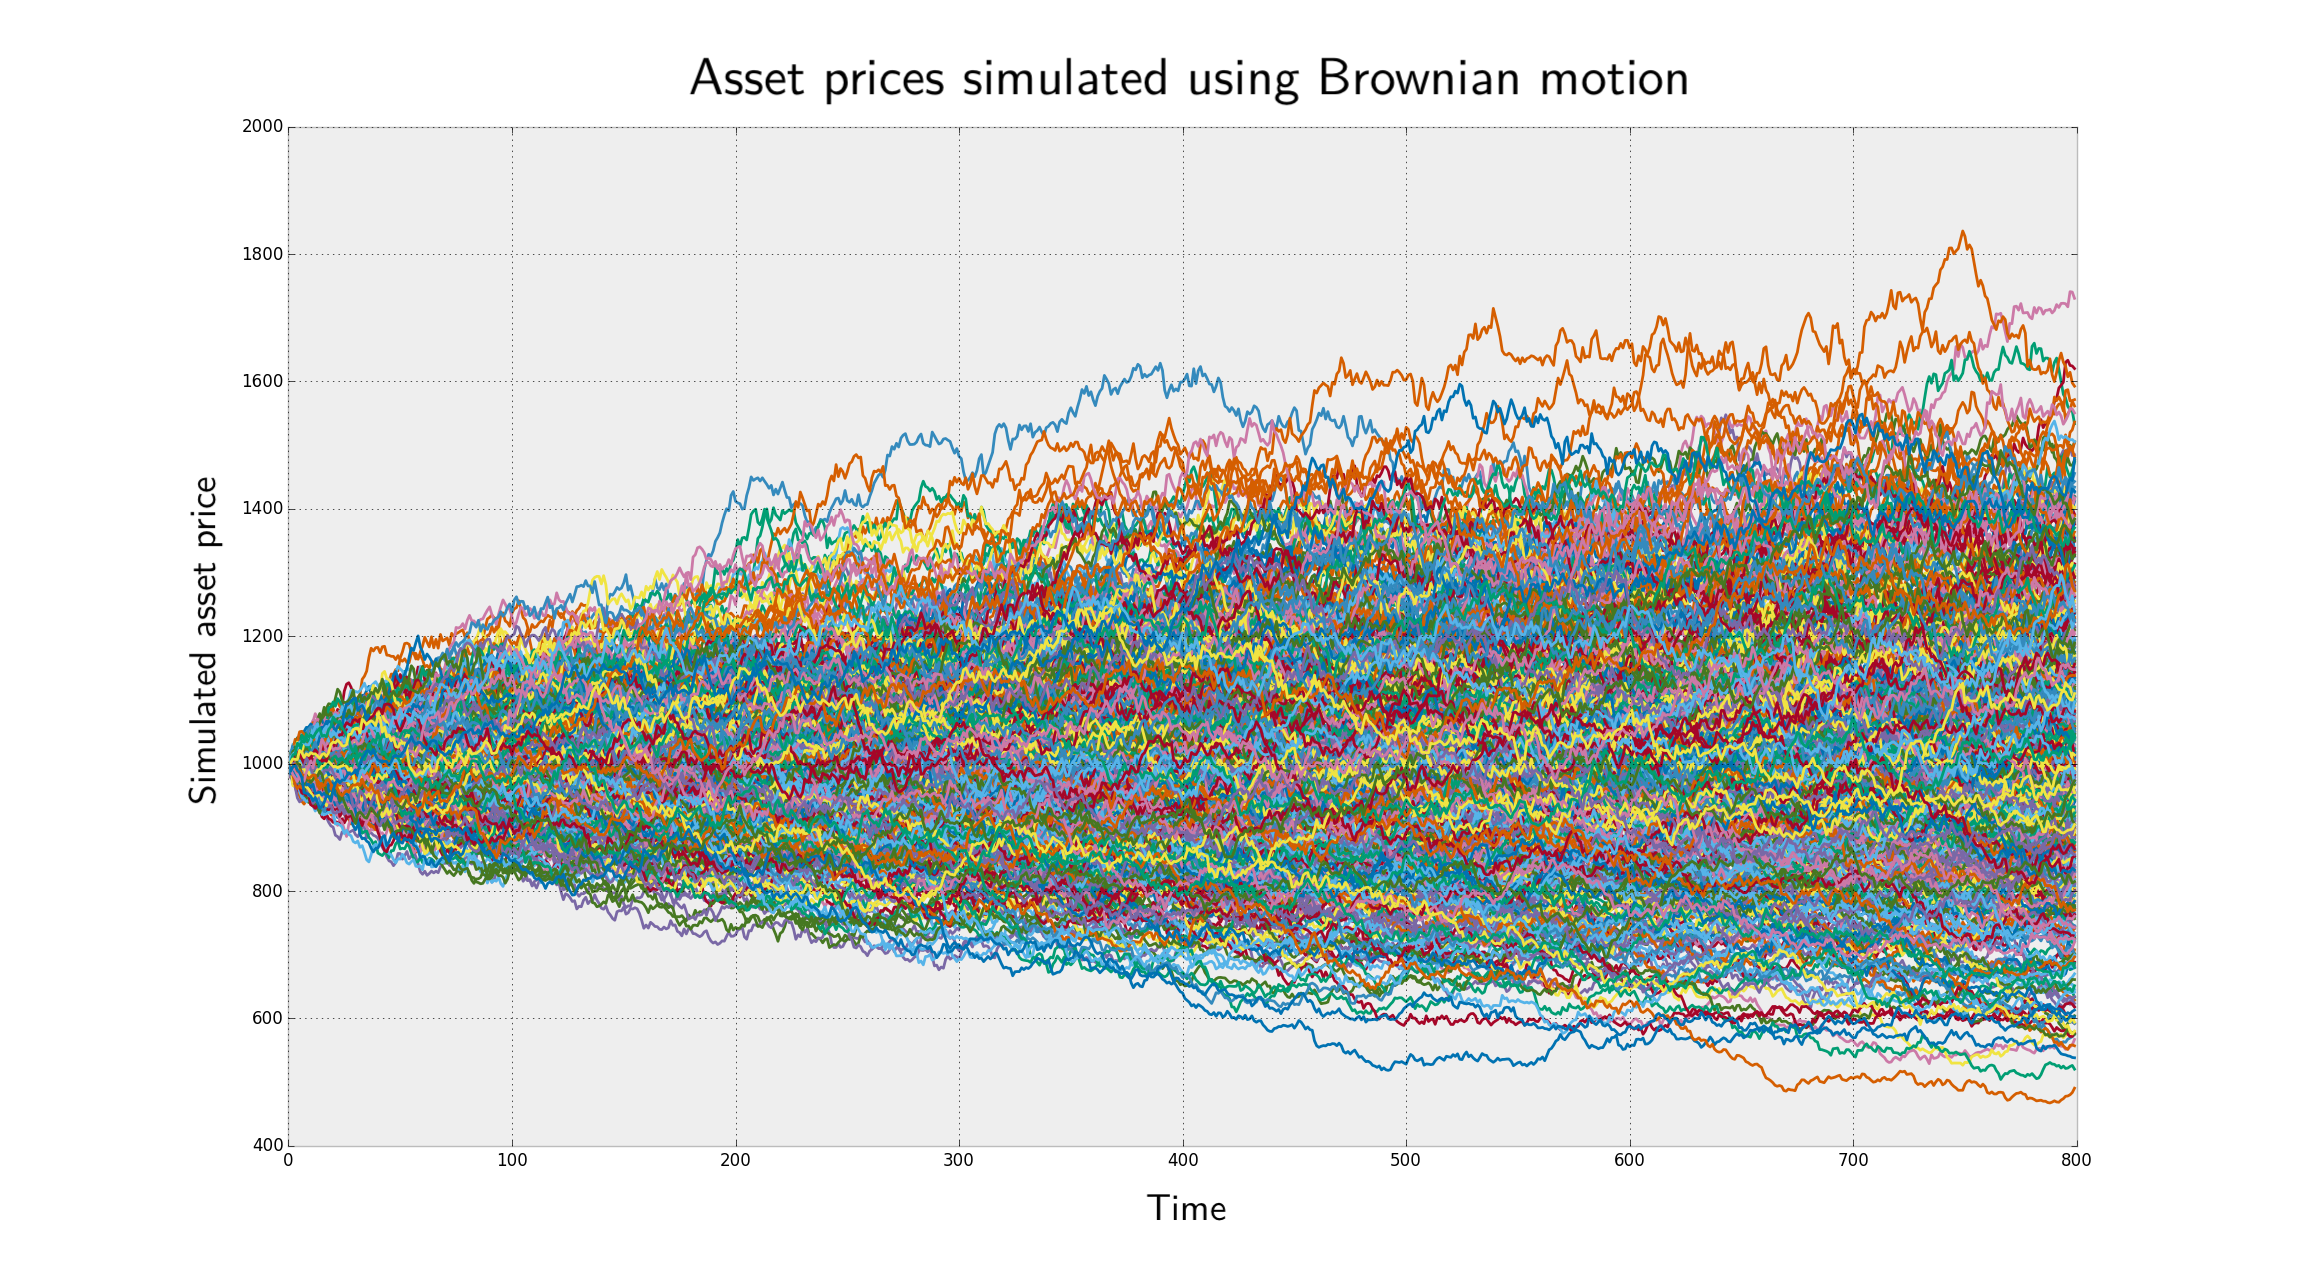
\includegraphics[scale=0.2]{fig/cover.png}
\end{center}
%---Frontpage End---%

\restoregeometry

\frontmatter
\tableofcontents
\vspace*{1cm}
\noindent {\small If you find any mistake or typo, please write at \href{mailto:matteo.bortoletto.2@studenti.unipd.it}{matteo.bortoletto.2@studenti.unipd.it}.
\begin{flushright}
{\small Matteo Bortoletto, 07/03/2020}
\end{flushright}}

\mainmatter
\chapter{Introduction} % 10 marzo 2020
\section{Forward contract} \lesson{1}{10/03/2020}
Let's assume that there are two counterparts interested in entering in a contract in the future. This means that at time $t=0$ they want to fix the price $K$ -- called \emph{strike price} -- of whatever (e.g. an asset, an interest rate, an exchange rate, the price of some good) at a future time $T$, called \emph{maturity} of the contract. The two counterparts are called:
\begin{itemize}
    \item \emph{long position}, which at time $T$ has to buy the asset at the price $K$ fixed at $t=0$, regardless the market price;
    \item \emph{short position}, which has to sell the asset at maturity
\end{itemize}
The price of the underlying asset at the current time $t$ is denoted as $S_t$ and it is known/measurable, whereas the price at time $S_T$ is a random variable. This type of contract is called \emph{forward contract}, since we are looking forward in the future. Because it costs nothing to enter into a forward contract, the payoff is also the trader’s total gain or loss from the contract.\\
What can we say about the payoff of the forward contract?
\begin{figure}
    \centering
    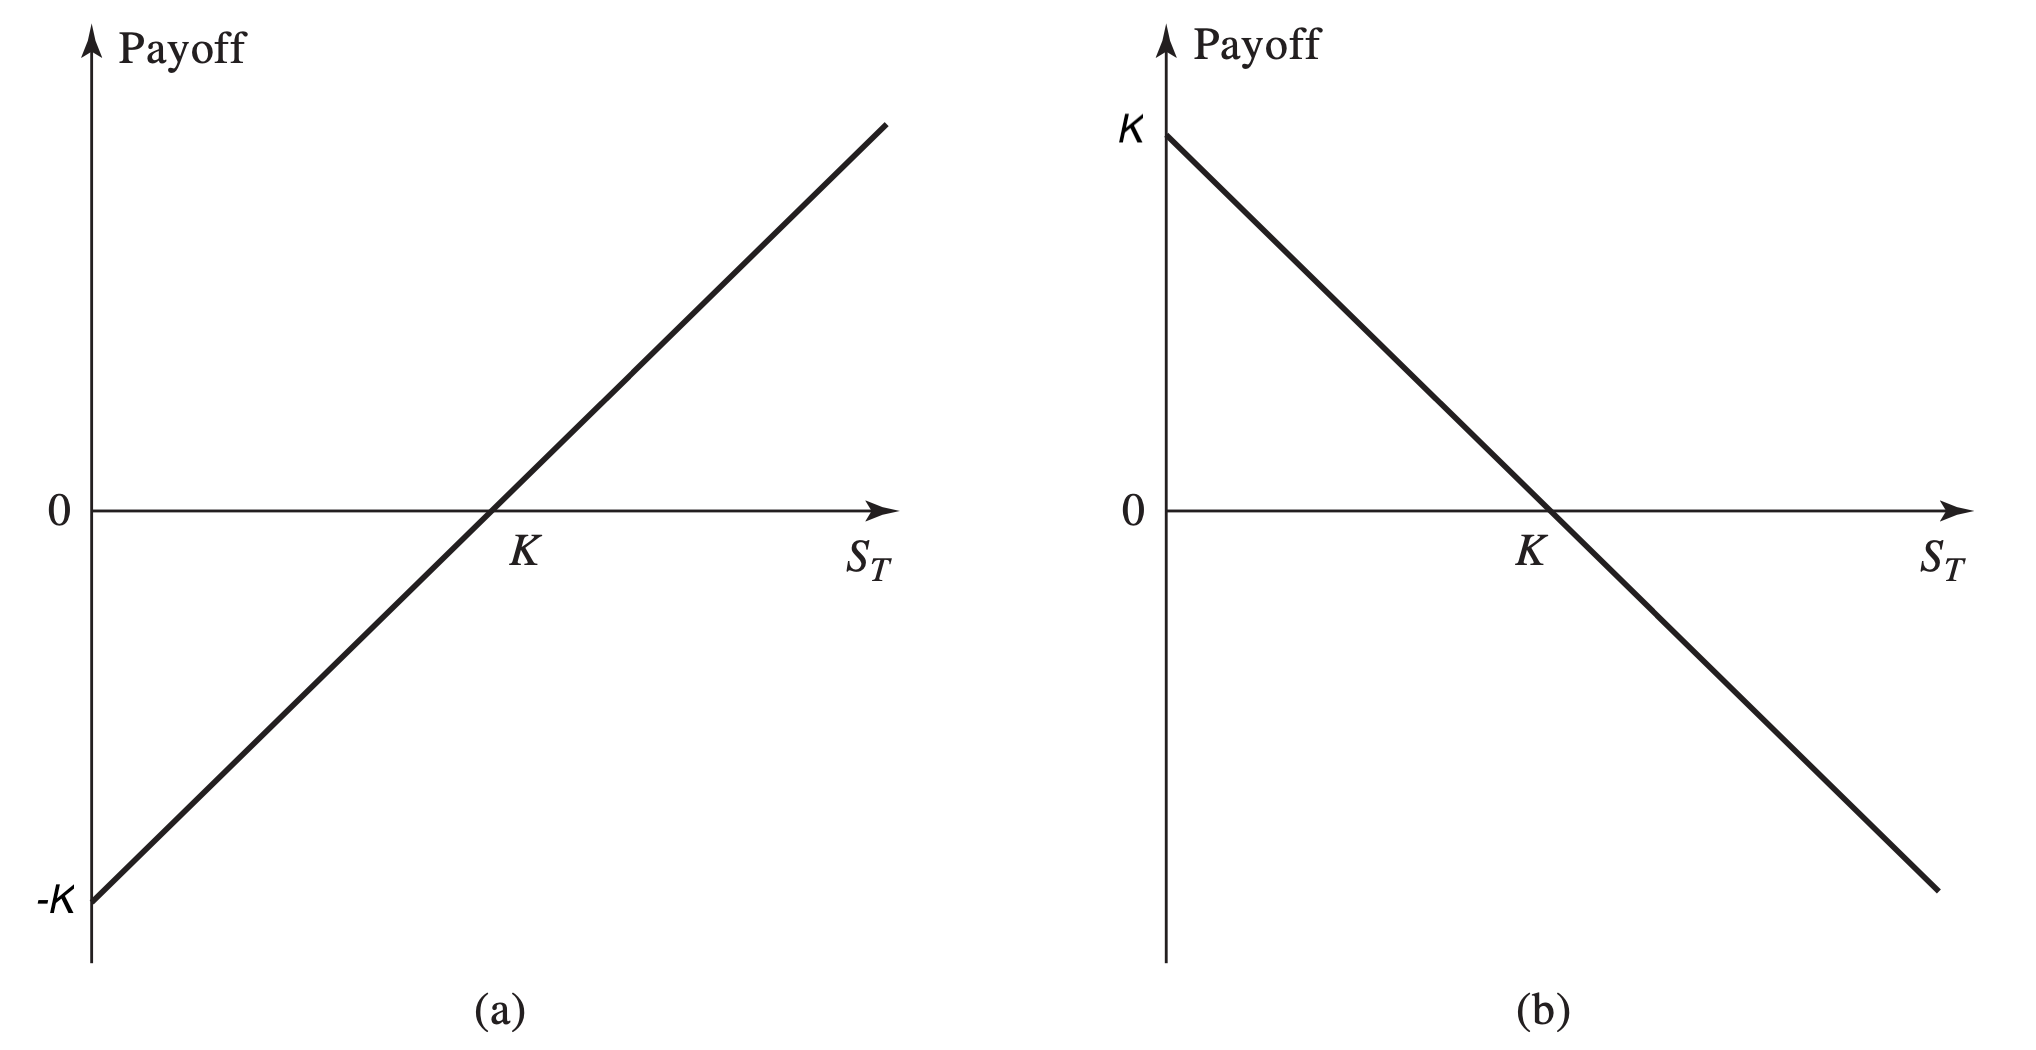
\includegraphics[scale=0.2]{fig/fc_payoff.png}
    \caption{Payoffs from forward contracts: (a) long position, (b) short position.}
    \label{fig:fc_payoff}
\end{figure}
If at time $T$ $S_T>K$ the long position is happy because it has the possibility to buy at $K$ and immediately sell at $S_T$ in the market, getting the payoff $S_T-K>0$. Conversely, if at time $T$ $S_T<K$ the long position is not happy because it buys at $K$ what is worth less in the market. For the short position the situation is symmetric. There are two important considerations:
\begin{enumerate}
    \item For the long position the loss is bounded and the gain is unbounded, whereas for the short position the loss is unbounded and the gain is bounded;
    \item If $K$ changes, for example if $K_2>K_1$, then the long position will not be happy because it wants $K$ to be as small as possible. So, it will not agree to enter in the contract.
\end{enumerate}
So, there is a trade-off between the two counterparts. Our purpose is to find the value of $K$ such that both parts will agree in entering the contract. To do that we have to avoid the presence of an \emph{arbitrage opportunity}, i.e. a possibility of making money for free, without risk (if there is an arbitrage opportunity then fixing a price is meaningless). Quantitatively, an arbitrage opportunity is defined as:
\begin{equation}
    V(t) = \begin{cases}
    0 & t = 0\\
    V_T\ge0 \mbox{ with } \mathbb{P}(V_T\ge0)=1 \mbox{ and } \mathbb{P}(V_T>0)>0 & t=T
    \end{cases}
\end{equation}
In order to avoid arbitrage opportunity we can construct the following portfolio:
\begin{enumerate}
    \item Take a long position in the forward contract. Entering the contract doesn't cost nothing and the payoff is $S_T-K$.
    \item Now we need a contract which gives $-S_T$ at $t=T$. One possibility is selling short: even if we don't have the underlying we borrow it from the broker and we sell it at the current price on the market, promising to re-buy it at time $t=T$ at the price $S_T$.
    \item Now we want to eliminate the $-K$ of step 1, so at $t=T$ we need $+K$ in any case, whatever happens to $S_T$. One possibility is to invest in the riskless market, which basically is the interest rate market\footnote{To be honest, it is not completely riskless, there is the default risk.}. There are two classical notions of interest rate:
    \begin{itemize}
        \item \emph{simple compounding}, which grows linearly in time: $1\to 1+TR$;
        \item \emph{exponential compounding}, which grows exponentially in time: $1\to e^{RT}$.
    \end{itemize}
    So we invest $-Ke^{-RT}$ in the riskless market and at the end we get $-Ke^{-RT}e^{RT}=-K$ changed of sign because at the beginning we spend and at the end we get.
\end{enumerate}
\begin{center}
    \begin{tabular}{lcc}\toprule
        Action & $t=0$ & $t=T$ \\\midrule
        Take a long position in the forward contract &  0 & $S_T-K$ \\
        Sell short & $+S_0$ & $-S_T$ \\
        Invest in the riskless market & $-Ke^{-RT}$ & $+K$ \\ \midrule\midrule
         & $S_0-Ke^{-RT}$ & $0$ \\\bottomrule
    \end{tabular}
\end{center}
In the end the sum at $t=0$ is $S_0-Ke^{-RT}$ and the sum at $t=T$ is zero. Since we want to avoid the presence of no arbitrage opportunity also the sum at $t=0$ has to be zero, otherwise there is an immediate arbitrage opportunity:
\begin{equation}
    S_0-Ke^{-RT} = 0 \quad\Rightarrow\quad K = S_0e^{RT}
\end{equation}
This is the value of $K$ such that both parts will agree in entering the contract.

\section{Options}
Options are derivatives based on the value of underlying securities, such as stocks. An option contract offers the buyer the opportunity to buy or sell -- depending on the type of contract they hold -- the underlying asset. There are two types of option:
\begin{itemize}
    \item a \emph{call} option gives the holder the right to buy the underlying asset by a certain date for a certain price;
    \item a \emph{put option} gives the holder the right to sell the underlying asset by a certain date for a certain price.
\end{itemize}

\subsection{Long call option}
In \emph{long call options} we have the possibility to buy the underlying at time $t=T$ at price $K$ decided at $t=0$. So, at maturity we will buy only if it is convenient.
\begin{figure}[h]
    \centering
    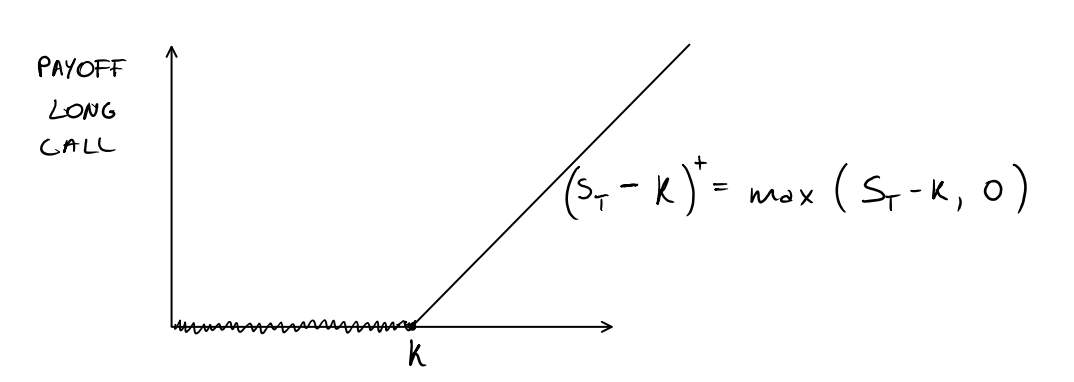
\includegraphics[scale=0.2]{fig/tmp/fig1a}
    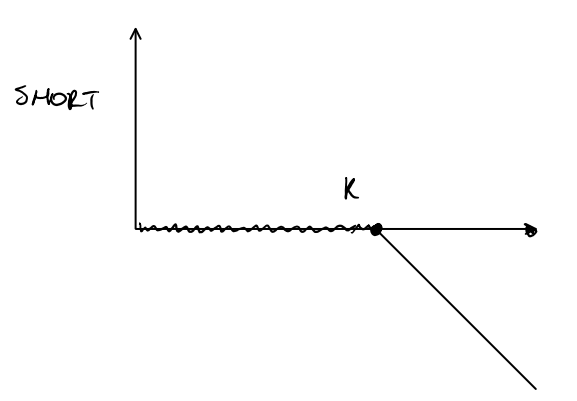
\includegraphics[scale=0.2]{fig/tmp/fig1b}
    \caption{Call option payoffs.}
    \label{fig:figura1}
\end{figure}
\newline Notice that now the payoff is no more linear. If we are in the short position at most we hope to get a zero payoff: nobody will accept this position. This means that the contract will have a price that the long position has to pay to the short position in order to enter the contract. In other words, it is as if the short position sells to the long position the possibility to buy.
\begin{figure}[h]
    \centering
    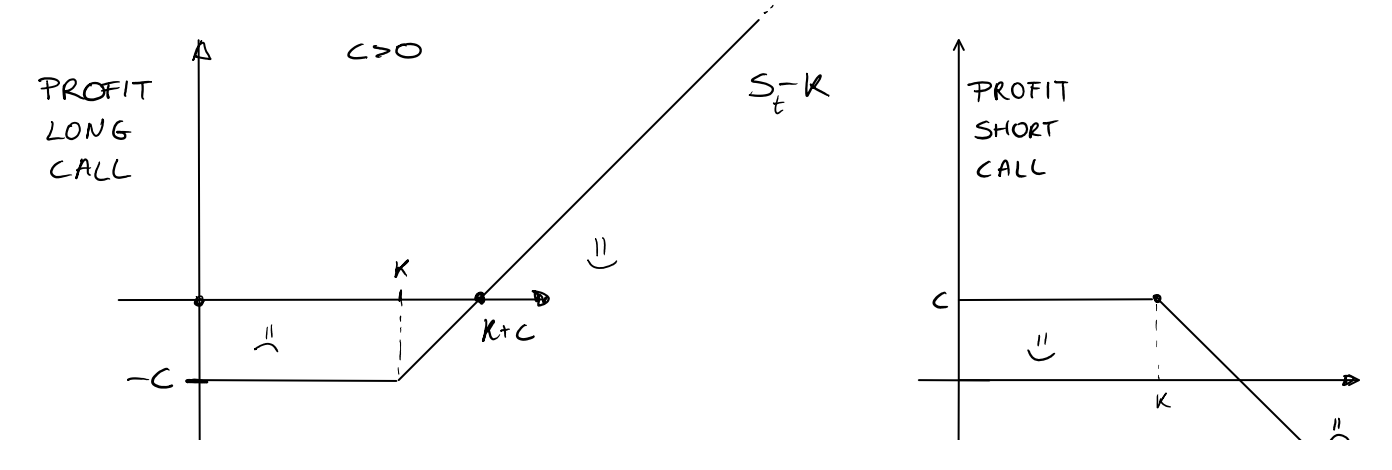
\includegraphics[scale=0.2]{fig/tmp/fig2}
    \caption{Call option profits.}
    \label{fig:figura2}
\end{figure}
\newline If we have different strike prices the corresponding costs will be different. For example, if we have $K_1<K_2$, since the probability to exercise the option corresponding to $K_2$ is smaller than the probability to exercise the option corresponding to $K_1$, then $c_1$ will be larger thank $c_2$:
\begin{equation*}
    K_1 < K_2 \quad\Rightarrow\quad c_1 > c_2
\end{equation*}
\begin{figure}[h]
    \centering
    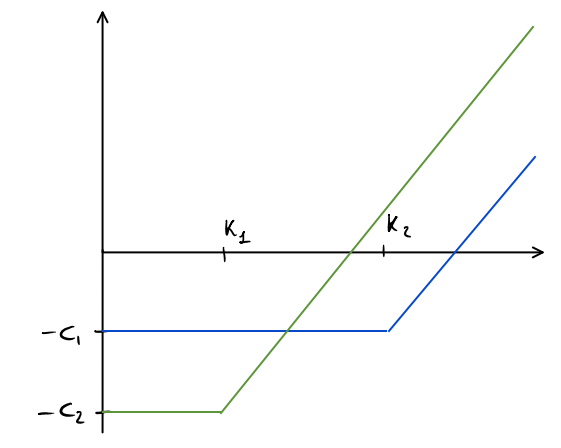
\includegraphics[scale=0.2]{fig/tmp/fig3}
    \caption{Costs for different strike prices.}
    \label{fig:figura3}
\end{figure}

\subsection{Long put option}
In \emph{long put options} we have the possibility to sell the underlying at time $t=T$ at price $K$ decided at $t=0$. So, at maturity we will sell to the counterpart only if it is convenient, i.e. if $S_T<K$\footnote{This is used, for example, by arabian countries which want to avoid that the price of crude oil goes below a certain level.}.
\begin{figure}[h]
    \centering
    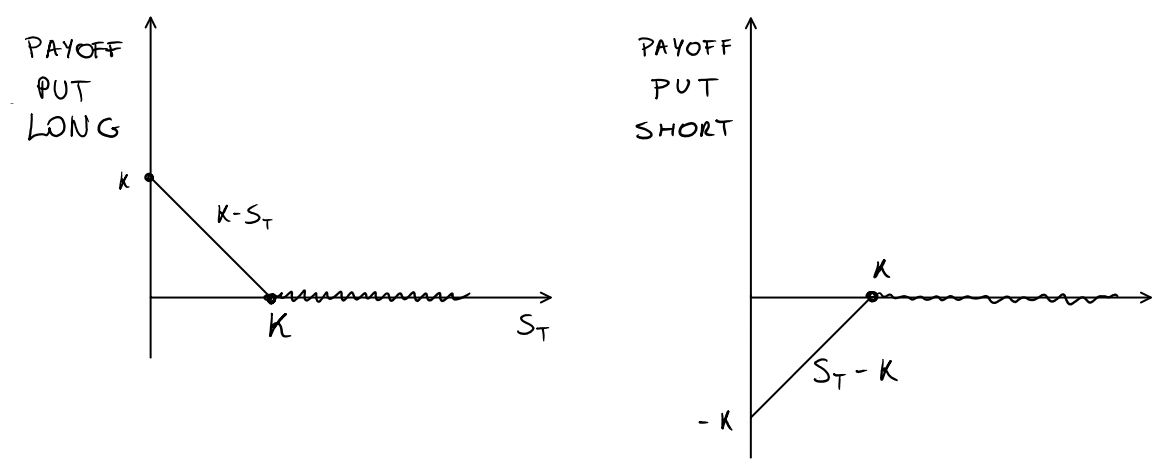
\includegraphics[scale=0.2]{fig/tmp/fig4}
    \caption{Put option payoffs.}
    \label{fig:figura4}
\end{figure}
In this case the short position has the obligation to buy. But there is no convenience in entering such a contract, so again there will be a cost to enter the contract as long position.
\begin{figure}[h]
    \centering
    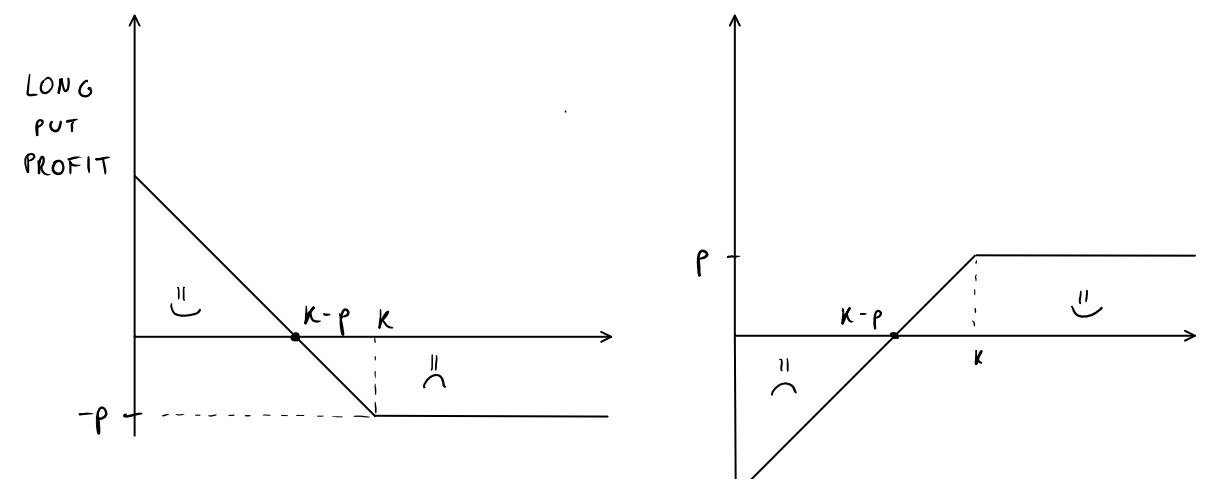
\includegraphics[scale=0.2]{fig/tmp/fig5}
    \caption{Put option profits.}
    \label{fig:figura5}
\end{figure}
If we have different strike prices, for example $K_1<K_2$, since the probability to exercise the option corresponding to $K_2$ is bigger than the probability to exercise the option corresponding to $K_1$, then $c_1$ will be smaller thank $c_2$:
\begin{equation*}
    K_1 < K_2 \quad\Rightarrow\quad c_1 < c_2
\end{equation*}

%\chapter{Lesson 12.03.2020} % 12 marzo 2020
\lesson{2}{12/03/2020}
Now we ask ourselves: which is the fair value of the price of this kind of contracts? In order to find it we need to introduce a probabilistic model. 

\chapter{Discrete time finance}
\section{Static binomial model}
The simplest probabilistic model is the \emph{static binomial model}. Suppose that we have an underlying with initial price $S_0$ at $t=0$ and which at time $t=T$ can assume two values, $Su$ and $Sd$ ($u>d$). The randomness arises from the fact that at time $t=0$ we don't know which will be the value at maturity, so we can say that $S_T$ is a two states random variable. \\
Now we would like to find which is the payoff of the call option, i.e.
\begin{equation}
    (S_T-K)^+ = \binom{(Su-K)^+}{(Sd-K)^+}
\end{equation}
Let's consider the following toy model: suppose to have an underlying which initial price is $S_0=100$ and $S_T=(Su,Sd)=(110,90)$ and consider a strike price $K=100$\footnote{If $K=S_0$ we say that the strike price is \emph{at the money}. If $K<S_0$ we say that it is \emph{in the money} and if $K>S_0$ it is \emph{out of the money}.}. The call payoff at the end will be
\begin{equation*}
    \binom{(110-100)^+}{(90-100)^+}=\binom{10}{0}
\end{equation*}
Which is the price of the call option at time $t=0$? Without knowing anything we can assume that the probability to get $Sd$ or $Su$ is the same, i.e. $1/2$, so the expected payoff at time $t=T$ is
\begin{equation*}
    10\cdot\dfrac{1}{2} + 0\cdot\dfrac{1}{2} = 5
\end{equation*}
Suppose that $T=1$ year. We are interested in the price today, so the natural way to get it is to discount this amount of money today. Assuming that the interest rate is exponential compounding with $R=2\%$ per year we have that the expected payoff at time $t=0$ is
\begin{equation*}
    e^{-RT}\mathbb{E}[\mbox{payoff}_T] = e^{-0.02\cdot1}\left(10\cdot\dfrac{1}{2} + 0\cdot\dfrac{1}{2}\right) 
\end{equation*}
Financially speaking, \textbf{this is completely wrong} because we are giving just our personal evaluation of the option price. Even using different probabilities for $Sd$ and $Su$ we would not have a price, because we are using a personal evaluation of the probability. A price has to be objective, not subjective. So, we have to completely forget this approach.\\
We have to find an objective way to determine, if not the price, at least an interval for the price. The idea is to perform the same reasoning we did for the price of the forward contract, i.e. to apply the no arbitrage principle. Let's write the payoff at time $T$ as 
\begin{equation*}
    \binom{f^u}{f^d}
\end{equation*}
The strategy is the following 
\begin{enumerate}
    \item We build up a strategy which replicates state of the nature by state of the nature all the values assumed by the random variable payoff. The idea is that the portfolio strategy has a value $V$ and the value of the portfolio at time $T$ is the payoff, i.e.
    \begin{equation*}
        V_T = \mbox{payoff}_T = \binom{f^u}{f^d}
    \end{equation*}
    Define $\alpha$ as the number of units of the underlying we have and $\beta$ as the number of obligations we have in the market (the possibility to land or borrow money), for example the \emph{zero coupon bond}, i.e. the contract that -- whatever happens to the market or to the underlying -- it gives the payoff equal to 1. There is not intermediate cash flow in the meanwhile. The terminal amount of money is denoted as \emph{notional}, which is typically computer in one hundred. So, a zero coupon bond is a contract that gives 100 at the end and at the beginning the value of the notional is $100e^{-RT}$. 
    \begin{example}{}{} 
    If the price of the zero coupon bond that gives 100 at the end is 99.5 today, and the time period between today and maturity is 3 months, we have
    \begin{equation*}
        99.5 = 100e^{-R\cdot3\mbox{ months}\frac{3}{12}}
    \end{equation*}
    where $3/12$ is due to the fact that typically the interest rate is computed in years. Inverting we get
    \begin{equation*}
        R = -\dfrac{12}{3}\ln\left(\dfrac{99.5}{100}\right)
    \end{equation*}
    \end{example}
    So we can invest in the risky market ($\alpha$) on in the interest rate/riskless market ($\beta$). Defining the portfolio strategy 
    \begin{equation*}
        V = \alpha S + \beta B
    \end{equation*}
    at the beginning we have 
    \begin{equation*}
        V_0 = \alpha S_0 + \beta\cdot1
    \end{equation*}
    and at the end we get 
    \begin{equation}
        V_T = \alpha S_T + \beta e^{RT} = \alpha\binom{Su}{Sd} + \beta\binom{e^RT}{e^RT}
    \end{equation}
    which is a random variable. This leads to a system of two equations:
    \begin{equation}
        \begin{cases}
            \alpha Su + \beta e^{RT} = f^u \\
            \alpha Sd + \beta e^{RT} = f^d
        \end{cases}
    \end{equation}
    which has solution (just subtract the second by the first)
    \begin{equation}
        \alpha = \dfrac{f^u-f^d}{Su-Sd}, \qquad \beta =  e^{RT}\left(f^d-Sd\dfrac{f^u-f^d}{Su-Sd}\right)
    \end{equation}
    \item At the end $V_T = \mbox{ payoff}_T$ with probability 1, because state of the nature by state of the nature they are the same. But if in the market there are two contracts with the same value at a certain time then necessarely they must share the same value also at the beginning: 
    \begin{equation*}
        V_0 = price_0(\mbox{payoff}_T)
    \end{equation*}
    This is due to the absence of arbitrage opportunity. In fact, suppose for example that $V_0>price_0(\mbox{payoff}_T)$. Then we can construct an arbitrary strategy. In order to do that we have to understand which is the anomaly in this situation. If at the beginning the portfolio is more expensive than the option, this means that it is too expensive, because with the option -- which is cheaper -- we can get the same value at the end. So, $V$ is the loser and the option is the winner and we can exploit the arbitrage by going long (buying) in the winner and going short (selling) in the loser.
    \begin{center}
        \begin{tabular}{lcc} 
            \toprule
                        & $t=0$        & $t=T$          \\\midrule
            Long option & -price$_0$   & $\alpha$payoff \\
            Short $V$   & $+V_0$       & $-V_T$         \\
            \midrule\midrule
             & $V_0-price_0>0$ & 0              \\\bottomrule
        \end{tabular}
    \end{center}
    If $V_0<price_0(\mbox{payoff}_T)$ we go short in the option and long in the portfolio. In the end, we get:
    \begin{equation}\label{V0}
        V_0 = price_0(\mbox{payoff}_T) = \alpha S_0 + \beta = \dfrac{f^u-f^d}{Su-Sd}S_0 + e^{RT}\left(f^d-Sd\dfrac{f^u-f^d}{Su-Sd}\right)
    \end{equation}\label{eq:bin_model}
\end{enumerate}
Notice that if using this simple model we end up with a pretty complicate expression, this means that this methodology doesn't lead to a technology which can be exploited in a realistic and more sophisticated framework. So we have to find a way to manipulate this expression in order to get something more readable.\\
Let's rewrite \eqref{eq:bin_model} as:
\begin{align}\label{readable}
    \notag V_0 
    &= 
    \alpha S_0 + \beta = \dfrac{f^u-f^d}{Su-Sd}S_0 + e^{RT}\left(f^d-Sd\dfrac{f^u-f^d}{Su-Sd}\right) \\
    \notag &=
    e^{-RT}\left[\dfrac{f^u-f^d}{u-d}+f^d-d\dfrac{f^u-f^d}{u-d}\right] \\
    \notag &=
    e^{-RT}\left[f^u\underbrace{\dfrac{e^{RT}-d}{u-d}}_{q}+f^d\underbrace{\dfrac{u-e^{RT}}{u-d}}_{1-q}\right] \\
    &=
    e^{-RT}\left[f^u q + f^d(1-q)\right]
\end{align}
We need $q>0$, otherwise there is an arbitrage opportunity. In fact, having a risky asset
\begin{equation*}
    S = \begin{cases}
        Su \\ Sd
    \end{cases} \overset{normalize}{\longrightarrow} \quad
    1 = \begin{cases}
        u \\ d
    \end{cases}
\end{equation*}
and a riskless asset
\begin{equation*}
    1 = \begin{cases}
        e^{RT} \\ e^{RT}
    \end{cases}
\end{equation*}
if $e^{RT}\le d$ it means that we can invest in the risky asset and at worst get the return $d$, but in any case -- even in the worst case -- the return is still greater than what we hope to get investing in the riskless asset. The risk asset becomes the winner! So we can exploit the arbitrage opportunity by tanking long position in the winner and short position in the loser.
\begin{center}
    \begin{tabular}{lcc} 
        \toprule
                            & $t=0$   & $t=T$                    \\\midrule
        Long S              & $-S_0$  & $+(S_0u,S_0d)$           \\
        Short \#S riskless   & $+S_0$  & $-(S_0e^{RT},S_0e^{RT})$ \\
                                                                 \midrule\midrule
                            & $0$     & $(S_0(u-e^{RT}),S_0(d-e^{RT}))>0$       \\\bottomrule
    \end{tabular}
\end{center}
We need also that $1-q>0$, which leads to $u<e^{RT}$. Again, if this does not hold we have an arbitrage opportunity (where this time the winner is the riskless asset). \\
So in the end I get eq. \eqref{readable}, which is way more readable now, because what I get is that the price price of the payoff is equal to the discounted value of a convex combination with positive probability weights, which is exactly an expected value:
\begin{equation}
    price_0(\mbox{payoff}_T) = e^{-RT}\mathbb{E}[\mbox{payoff}_T]
\end{equation}
This expression looks the same as the one we said was completely wrong. Not exactly: the crucial difference is that I don't use my subjective probability but only elements which are present in the market. In particular, the probability weight $q$ is not chosen by us, but it depends on market parameters, i.e. the fact that the underlying goes up and down without touching any probability or interest rate. To stress the fact that the probability is not subjective, we write
\begin{equation}\label{price}
    price_0(\mbox{payoff}_T) = e^{-RT}\mathbb{E}^{\Qmeas}[\mbox{payoff}_T]
\end{equation}
where 
\begin{equation}
    Q \to \binom{q}{1-q}
\end{equation}
is known as \emph{risk neutral probability measure}.\\
So, in the end, we found a metodology for the pricing:
\begin{enumerate}
    \item Which is the payoff$_T$ I'm interested to price?
    \item Compute $q = \frac{e^{RT}-d}{u-d}$;
    \item Compute the price using \eqref{price}.
\end{enumerate}

\subsection{Implementation}\label{sec:impl}
Let's talk about implementation. Even if the model is very stylized, it would be nice to understand if it is possible to apply it concretely is some cases. We need to specify $u$ and $d$, which values are related to the volatility of the price, i.e. to the variability of the underlying. If $u>>d$ we are confident on the fact that future realizations of the underlying will increase, if $u\sim d$ we are not confident on the fact that future realizations of the underlying will increase. \\
It would be nice to be able to estimate $u$ and $d$ starting from real data. In order to do that we have to consider some historical series of daily closing prices $(S_{-n},\dots,S_0)$ and switch to returns (since we want $u$ and $d$):
\begin{equation}
    \mbox{Return}_t = R_t = \dfrac{S_t-S_{t-1}}{S_{t-1}} = \ln\left(\dfrac{S_t}{S_{t-1}}\right)
\end{equation}
So we get a vector $(R_{-n-1},\dots,R_0)$. Then we have to compute the standard deviation
\begin{equation}
    \sigma_{daily} = \sqrt{\dfrac{\sum^{n-1}_{i=0}(R_i-\Bar{R})^2}{n-1}}
\end{equation}
which is called \emph{daily volatility}. $u$ and $d$ are given by
\begin{equation}
    u = e^{\sigma_{year}\sqrt{T}}, \qquad d = e^{-\sigma_{year}\sqrt{T}}
\end{equation}
where $\sigma_{year} = \sigma_{daily}\sqrt{250}$ (250 are the opening days in the market) and $T$ is measured is years (so if we have $T=3$ months we have to put $T=3/12$). Once we have $u$ and $d$ we can implement our binomial model
\begin{remark}\label{remark}
    In principle we can price whatever. If we consider that the payoff is the underlying itself
    \begin{equation}
        \mbox{payoff}_T = S_T
    \end{equation}
    i.e. the payoff gives one unit of underlying at the end, the corresponding price of this particular payoff is given by    \eqref{price}:
    \begin{align}
        \notag e^{-RT}\mathbb{E}^{\Qmeas}[(S_T)] &= e^{-RT}(qSu+(1-q)Sd) = e^{-RT}S(qu+(1-q)d) \\
        &= e^{-RT}S\left(u\frac{e^{RT}-d}{u-d}+d\frac{u-e^{RT}}{u-d}\right) = S_0
    \end{align}
    which makes sense, because the market value of the underlying today is exactly what we observe today, i.e. the quoted price of the underlying. So we can say the methodology is consistent. But there is something more, in the sense that if we write
    \begin{equation}\label{S0}
        \mathbb{E}^{\Qmeas}[e^{-RT}(S_T)] = S_0e^{-R\cdot0} = S_0
    \end{equation}
    we see that the expected value is the same as the value that we observe. This is a very stylized case of the property of a \emph{martingale}. However, this is not properly a martingale (since there is no stochasticity), but just a preliminary intuition of the fact that ``the process $S_te^{-RT}$, i.e. the discounted asset, will be a $\Qmeas$-martingale".
\end{remark}
%\chapter{Lesson 13.03.2020} % 13 marzo 2020
\section{Hedging}\lesson{3}{13/03/2020}
We saw that the price of a given payoff is given by \eqref{fig:fc_payoff}, so we solved the problem of pricing. This completely solve the problem for the long position, who wants to know which is the correct price to pay to the short position in order to get the payoff at the end. \\
Now we have to solve the problem for the short position. One possibility is to sell the option (possibility) and hope that the market goes in the right direction, but this it is not a good strategy. For the short position we have to build up a portfolio which value at time $T$ is exactly the payoff we have to give to the long position. This problem is known as \emph{hedging}. The strategy is the following:
\begin{enumerate}
    \item Solve the pricing problem
    \item Take $\alpha$ shares, i.e. the number of shares that we have to hold in our portfolio in order to replicate the payoff:
    \begin{equation}
        \alpha = \dfrac{f^u-f^d}{Su-Sd} =  \dfrac{\Delta\mbox{payoff}}{\Delta S} \equiv \Delta
    \end{equation}
    This quantity is know in general as \emph{delta} and it represents the amount of underlying we have to get in the portfolio in order to replicate the payoff of the option.
    \item Invest into the riskless market, taking $\beta$ according to \eqref{V0}:
    \begin{equation}
        \beta = price_0-\Delta S_0
    \end{equation}
\end{enumerate}
\begin{example}{}{}
Consider again the toy model where we have an underlying which initial price is $S_0=100$, $T=1$ year, $S_T=(Su,Sd)=(110,90)$, a strike price $K=100$ and an interest rate of $1\%$ per year. Then we have 
\begin{equation*}
    u = \dfrac{110}{100} = 1.1 \qquad d = \dfrac{90}{100} = 0.9
\end{equation*}
The corrisponding $q$ is 
\begin{equation*}
    q = \dfrac{e^{RT}-d}{u-d} = \dfrac{e^{0.01}-0.9}{1.1-0.9} = 0.555
\end{equation*}
Now we are able to compute the price of the call:
\begin{equation}
    price_0(\mbox{call}) = e^{-RT}(10q+ 0(1-q)) = 10qe^{-RT} = 5.44
\end{equation}
This is the market price coherent with the no arbitrage principle of a \colorbox{magenta}{promise} that can give a payoff between 10 and 0. So, in order to use the replicating portfolio strategy, the short position has to sell the option for a price $\mbox{price}^{mkt}>5.44$. The income of $\mbox{price}^{mkt}-5.44$ can be put in the pocket, but we have to use 5.44 in order to build up the hedging strategy, which consists in taking
\begin{equation*}
    \Delta = \dfrac{f^u-f^d}{Su-Sd} = \dfrac{10-0}{110-90} = 0.5
\end{equation*}
shares in the risky market and 
\begin{equation*}
    \beta = price_0-\Delta S_0 = 5.44 - 0.5\cdot100 = -44.56
\end{equation*}
For example, if the underlying is worth \EUR{100}, I have to invest \EUR{50} in the risky market. But if we are in the short position we don't have \EUR{50}, because we receive only \EUR{5.44} from the long position. So we take the \EUR{5.44} and we borrow \EUR{44.56} from the riskless market in order to invest in the risky market\footnote{In the real market you don't buy one $\Delta = 0.5$ but you consider a package of two options and the global hedging.}. \\
In this kind of business we usually get slightly more than price$_0$. For example, if price$_0$ = \EUR{5.44} we would expect to get something like \EUR{5.54}. Notice that for a personal business of \EUR{0.10} we are obliged to construct a trading strategy which involves an investment of \EUR{50} in the risky market and \EUR{44.56} in the riskless market, so we have to move a huge amount of money compared to what we get at the end. That's why it is very important to be precise in the hedging strategy.
\end{example}

\section{Dividends}
A \emph{dividend} is a payment made by a corporation to its shareholders. The idea is that if we own one asset sometimes the corresponding corporate decides to give us -- in addition to the market value of our asset -- some extra bonus. \\
Consider a binomial model in which we have and underlying with initial value $S$ and final values given by the terminal values $Su,Sd$ plus a bonus:
\begin{equation}
    S \to \begin{cases} 
    Su + Se^{\delta T} \\ Sd + Se^{\delta T} 
    \end{cases}
\end{equation}
where $\delta$ is called \emph{dividend rate} and in general is a random variable. In such cases we say that the price is \emph{cum dividend}, whereas if there is no dividend the price is \emph{ex dividend}. We can repeat the same arguments we did before for the price ex dividend introducing the dividend as a shift of the price of the underlying. The probability weight becomes
\begin{equation}
    q = \dfrac{e^{RT}-(d+e^{\delta T})}{u-d}
\end{equation}
\begin{remark}
    Recall that in Remark \ref{remark} we found a stylized case of martingale. Now we have 
    \begin{equation}
        \mathbb{E}^{\Qmeas}[S_T] = S_0(e^{RT}-e^{\delta T})
    \end{equation}
    so it is not true anymore that discounted assets are constant in expected value.
\end{remark}

\subsection{Put-call parity}\label{putcallparity}
One interesting thing is that it is possible to deduce the implicit dividend policy of a corporate -- which usually is private -- from the prices quoted in the market. In order to do that we use the \emph{put-call parity}, which is a link between the put and the call prices. \\
Start by considering no dividends. Notice that any number can be written as positive part minus negative part:
\begin{equation*}
    x = x^+ - x^- = x^+ - (-x)^+ 
\end{equation*}
So, we can write
\begin{equation}
    S_T - K = \underbrace{(S_T - K)^+}_{call} - \underbrace{(K - S_T)^+}_{put}
\end{equation}
Now we use the linearity of expected value:
\begin{equation*}
    \mathbb{E}^{\Qmeas}[S_T-K] = \mathbb{E}^{\Qmeas}[(S_T-K)^+] - \mathbb{E}^{\Qmeas}[(K-S_T)^+]
\end{equation*}
and multiply both sides for the discounted value:
\begin{equation*}
    e^{-RT}\mathbb{E}^{\Qmeas}[S_T-K] = \underbrace{e^{-RT}\mathbb{E}^{\Qmeas}[(S_T-K)^+]}_{call_0} - 
    \underbrace{e^{-RT}\mathbb{E}^{\Qmeas}[(K-S_T)^+]}_{put_0}
\end{equation*}
where we recognized the initial price of the call and of the put. Then we use the property ${\mathbb{E}}[aX+b]=a{\mathbb{E}}[X]+b$:
\begin{equation*}
    e^{-RT}\mathbb{E}^{\Qmeas}[S_T-K] = e^{-RT}\mathbb{E}^{\Qmeas}[S_T] - Ke^{-RT} = \mathbb{E}^{\Qmeas}[e^{-RT}S_T] - Ke^{-RT} \overset{\eqref{S0}}{=} S_0 - Ke^{-RT}
\end{equation*}
In the end, we get:
\begin{equation}\label{put-call}
    S_0 - Ke^{-RT} = call_0 - put_0 \qquad\Rightarrow\qquad put_0 = call_0 - S_0 +  Ke^{-RT}
\end{equation}
Now consider the presence of dividends the put-call parity becomes
\begin{equation}\label{put-call-div}
    put_0 = call_0 - S_0 +  Ke^{-RT} + S_0e^{(\delta - R)T}
\end{equation}
that means that if for the same asset there is a market of put options and call options with a certain maturity, then we consider the list of the quoted prices of the put and of the call and use eq. \eqref{put-call-div} to find $\delta$.

\section{Market completeness}
Let's consider the following assumptions:
\begin{enumerate}
    \item short positions and fractional holdings of the underlying are allowed;
    \item there is no \emph{bid-ask spread}, i.e. there is no difference between the prices quoted for an immediate sale (ask) and an immediate purchase (bid) for an underlying;
    \item there are no transaction costs;
    \item there is a perfectly liquid market, i.e. there is the possibility to buy or sell an unlimited quantity of an underlying.
\end{enumerate}
\begin{definition}[Reachable contingent claim]
    A contingent claim\footnote{A contingent claim is a derivative whose future payoff depends on the value of another “underlying” asset, or more generally, that is dependent on the realization of some uncertain future event.} $x\in\mathbb{R}^2$ is \emph{reachable} if there exists a portfolio $h(\alpha,\beta)$ with terminal value $V^h_T=x$ almost surely (i.e. with probability 1). In this case $h$ is called hedging portfolio.
\end{definition}
\begin{definition}[Complete market]
    If all the claims are reachable, the market is \emph{complete}.
\end{definition}
So, in a complete market it is possible to replicate all the possible random variables, i.e. all the possible contracts.
\begin{proposition}\label{prop1}
    If a claim $x$ is reachable with $h$ and there is absence of arbitrage opportunity, then the price of $x$ is
    \begin{equation}
        price_0(x) = V_0^h.
    \end{equation}
\end{proposition}
\begin{remark}
    If a claim $x$ is reachable than Prop. \ref{prop1} holds also in an incomplete market.
\end{remark}
\begin{proposition}\label{prop2}
    The binomial model with $d<e^{RT}<u$ is arbitrary free and complete.
\end{proposition}
\noindent So, in a static binomial model it is possible to price everything. The next step is to consider a dynamic model.

\section{The multi period case}
We want to generalize the binomial model
\begin{equation*}
    S\to\begin{cases}
    Su \\ Sd
    \end{cases}
\end{equation*}
For example we can introduce a third possible realization of the underlying, obtaining a trinomial model:
\begin{equation*}
    S\to\begin{cases}
    Su \\ Sm \\ Sd
    \end{cases}
\end{equation*}
In this case, since we have only two tools in our investment strategy (the risky and rikless markets) if, for example, we want to replicate a call option, the payoff is
\begin{equation*}
    (S_T-K)^+ = \left(\begin{matrix}
        (Su-K)^+ \\ (Sm-K)^+ \\ (Sd-K)^+
    \end{matrix}\right)
\end{equation*}
and we have to solve three equations with two unknowns, which -- apart from special cases -- is impossible to solve. So, just adding one more possible outcome leads to uncomfortable consequences in terms of pricing methodology, because our model is no more complete. We have the possibility to invest in the risky market and in the riskless market in order to follow the fluctuations of something which can take three values, so the underlying fluctuates too much. We need another instrument to follow the flutuations of the underlying, for example an extra underlying $S'$, but things become complicated. It is much more convenient to introduce a dynamic framework. For example, consider the following tree.
\begin{center}
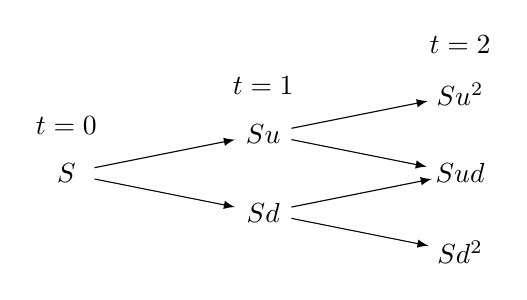
\begin{tikzpicture}[
                   grow = right,
edge from parent/.style = {draw,-latex},
         label distance = 1.5mm,
      every node/.style = {minimum width=2em, inner sep=3pt},
         level distance = 25mm,
       sibling distance = 10mm,
                     ]
\node[label=90:{$t=0$}] {$S$}
    child {node {$Sd$}
        child {node {$Sd^2$}
            %child {node {40}}
            %child {node {20}}
                }
        child {node {}}%<---------------- already printed
            }
    child {node[label=90:{$t=1$}] {$Su$}
        child {node {$Sud$}
            %child {node {}}%<------------ already printed
            %child {node {0}}
                }
        child {node[label=90:{$t=2$}] {$Su^2$}
            %child {node {}}%<------------ already printed
            %child {node[label=90:{$t=3$}] {0}}
                }
                };
\end{tikzpicture}
\end{center}
In this case the tree is stationary, i.e. $u$ and $d$ are always the same for every $t$. This tree is called \emph{recombining tree} or \emph{lattice}. Computationally speaking this is an advantage because if we have $n$ steps then the terminal values are $n+1$, so the number of all the possible realizations remains linear with respect to time.\\
Conversely, if we consider a non-recombining tree, like
\begin{center}
\tikzstyle{level 1}=[level distance=25mm, sibling distance=13mm]
\tikzstyle{level 2}=[level distance=25mm, sibling distance=8mm]
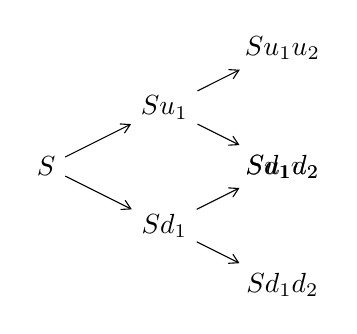
\begin{tikzpicture}[grow=right,->,>=angle 60]
  \node {$S$}
    child {node {$Sd_1$}
      child {node {$Sd_1d_2$}
      }
      child {node{$Sd_1u_2$}
      }
    }
    child {node {$Su_1$}
      child {node{$Su_1d_2$}
      }
      child {node{$Su_1u_2$}
      }
    };
\end{tikzpicture}
\end{center}
for $n$ steps we have $2^n$ possible realizations, which for large $n$ is impossible to manage.\\
The decision between combining and non-combining tree is crucial, and it should be motivated by some financial argument. Why should we use non-recombining trees? What we observe in the market is that when $S$ goes up the volatility is low, whereas when the market decreases there is an increase of the volatility.
\begin{center}
    \colorbox{green}{fig6}
\end{center}
This is the reason why it could be interesting to consider a non-recombining tree. However, if we choose this kind of model there is a problem in the implementation. Recall that in the binomial model $u$ and $d$ are given by $(u,d)\sim e^{\pm\sigma\sqrt{T}}$: the problem is we have only one historical series, and if the parameters vary step by steps it is impossible to estimate them. So we drop this model and we use a recombining tree.
\begin{remark}
    Sometimes it is not possible to use a recombining tree because there are same contracts which payoff depends on the whole past history of the underlying. So, in these cases it is not enough to take a picture of the underlying at the maturity. For example, in the 70s some manipulations have been used in order to rise the price of crude oil immediately before the maturity and then exercise the call option, buying at $K<S_T$ and getting $S_T-K>0$. In order to avoid this kind of manipulations, contracts which payoff depends on the whole past history of the underlying -- called \emph{asian options} -- have been introduced. Asian options payoff is given by
    \begin{equation}
        \mbox{payoff}_T = \left(\dfrac{1}{T}\int^T_0 S_s\,ds-K\right)^+
    \end{equation}
\end{remark}
%\chapter{Lesson 18.03.2020} % 18 marzo 2020
\lesson{4}{18/03/2020}
\noindent Since we are interested in pricing simple options, we consider a \emph{stationary binomial recombining tree} or \emph{lattice}, i.e. a model in which the way the underlying goes up and down increases or decreases is always the same.

\section{Binomial lattice}
\subsection{Pricing options}
Consider the following binomial lattice:
\begin{center}
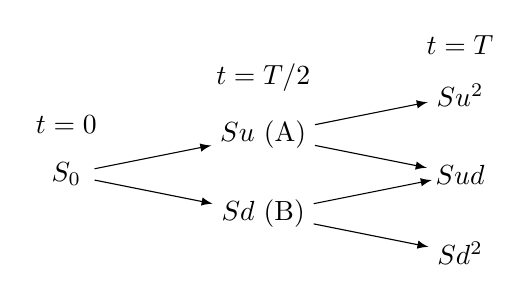
\begin{tikzpicture}[
                   grow = right,
edge from parent/.style = {draw,-latex},
         label distance = 1.5mm,
      every node/.style = {minimum width=2em, inner sep=3pt},
         level distance = 25mm,
       sibling distance = 10mm,
                     ]
\node[label=90:{$t=0$}] {$S_0$}
    child {node {$Sd$ (B)}
        child {node {$Sd^2$}
            %child {node {40}}
            %child {node {20}}
                }
        child {node {}}%<---------------- already printed
            }
    child {node[label=90:{$t=T/2$}] {$Su$ (A)}
        child {node {$Sud$}
            %child {node {}}%<------------ already printed
            %child {node {0}}
                }
        child {node[label=90:{$t=T$}] {$Su^2$}
            %child {node {}}%<------------ already printed
            %child {node[label=90:{$t=3$}] {0}}
                }
                };
\end{tikzpicture}
\end{center}
and a call option, whose payoff is the random vector
\begin{equation*}
    \mbox{payoff}_T = \left(
    \begin{matrix}
        (Su^2-K)^+ \\ (Sud-K)^+ \\ (Sd^2-K)^+
    \end{matrix}
    \right)
    =
    \left(
    \begin{matrix}
        f^{u^2} \\ f^{ud} \\ f^{d^2}
    \end{matrix}
    \right)
\end{equation*}
The problem is always the same: how much do we have to pay at time $t=0$ in order to get this payoff at time $t=T$?\\
Suppose that we are in node (A). According to the risk neutral methodology, the value of the relative sub-payoff is given by
\begin{align}
    \notag Value_A\left(\binom{f^{u^2}}{f^{ud}}\right)
    &=
    \notag e^{-R\frac{T}{2}}\mathbb{E}^{\Qmeas}\left(\left.\binom{f^{u^2}}{f^{ud}}\right|\mbox{(A)}\right)\\
    &=
    e^{-R\frac{T}{2}}(qf^{u^2}+(1-q)f^{ud})
\end{align}
where
\begin{equation}\label{qT2}
    q = \dfrac{e^{R\frac{T}{2}}-d}{u-d}
\end{equation}
Notice that in this case the expected value is a conditional expected value. In analogy, in the node (B) we have
\begin{equation}
    Value_B\left(\binom{f^{ud}}{f^{d^2}}\right) = e^{-R\frac{T}{2}}(qf^{ud}+(1-q)f^{d^2})
\end{equation}
Now, we can compute the initial price of the whole payoff:
\begin{align}
    \notag price_0\left(
    \begin{matrix}
        f^{u^2} \\ f^{ud} \\ f^{d^2}
    \end{matrix}
    \right)
    &=
    price_0\left(\begin{matrix}
        Value_A \\  Value_B
    \end{matrix}\right)\\
    %\binom{Value_{(A)}}{Value_{(B)}} \\
    &=
    \notag e^{-R\frac{T}{2}}\mathbb{E}^{\Qmeas}\left[\left(
    \begin{matrix}
        Value_A \\  Value_B
    \end{matrix}\right)
    %\binom{Value_{(A)}}{Value_{(B)}}
    \right]\\
    &=
    \notag e^{-R\frac{T}{2}}(q Value_A+(1-q)Value_B)\\
    &=
    \notag e^{-R\frac{T}{2}}\left[q\left(e^{-R\frac{T}{2}}(qf^{u^2}+(1-q)f^{ud})\right) + (1-q)\left(e^{-R\frac{T}{2}}(qf^{ud}+(1-q)f^{d^2})\right)\right]\\
    &=
    e^{-RT}[q^2f^{u^2}+2q(1-q)f^{ud}+(1-q)f^{d^2}]
\end{align}
Notice that the three coefficients are positive and their sum gives 1, so again we obtained a convex combination of elements, i.e. an expected value:
\begin{equation}
    price_0
    \left(
    \begin{matrix}
        f^{u^2} \\ f^{ud} \\ f^{d^2}
    \end{matrix}
    \right)
    = e^{-RT} \mathbb{E}^{\Qmeas}
    \left[
    \left(
    \begin{matrix}
        f^{u^2} \\ f^{ud} \\ f^{d^2}
    \end{matrix}
    \right)
    \right]
    = e^{-RT}\mathbb{E}^{\Qmeas}[\mbox{payoff}_T]
\end{equation}
The formula has the same form as before but it must be contextualized as the expectation under the risk neutral probability measure
\begin{equation}
    Q \sim
    \left(
    \begin{matrix}
        q \\ 2q(1-q) \\ q^2
    \end{matrix}
    \right)
\end{equation}

\subsection{Hedging}
We now want to implement the corresponding hedging portfolio, i.e. the replicating portfolio which allows the short position to construct the payoff for the long position. \\
First we have to solve the pricing procedure for all the intermediate nodes, in fact hedging is a forward procedure. Then, the number of shares we have to put in our portfolio is
\begin{equation}
    \Delta_0 = \dfrac{Value_A-Value_B}{Su-Sd}
\end{equation}
and the corresponding investment in the riskless market is
\begin{equation}
    \beta_0 = p_0-\Delta_0S
\end{equation}
where $p_0 = V_0 = price_0$. This is the initial step. Now we have to consider the intermediate step, according to the possible values of the underlying:
\begin{equation}
    \Delta_A = \dfrac{f^{u^2}-f^{ud}}{Su^2-Sud}, \qquad \Delta_B = \dfrac{f^{ud}-f^{d^2}}{Sud-Sd^2}
\end{equation}
Now we have
\begin{equation*}
    Value_A = \Delta_ASu+\beta_Ae^{R\frac{T}{2}}, \qquad Value_B = \Delta_BSd+\beta_Be^{R\frac{T}{2}}
\end{equation*}
so the investment in the riskless market is
\begin{equation}
    \beta_A = (Value_A-\Delta_ASu)e^{-R\frac{T}{2}}, \qquad \beta_B = (Value_B-\Delta_BSd)e^{R\frac{T}{2}}
\end{equation}
So, in a dynamic binomial model, also the hedging is dynamic. This is obvious, since we can exploit the possibility to change our strategy according to the fluctuations of the underlying.

\subsection{Dynamic interest rates}
\begin{remark}
There are two possible riskless assets:
\begin{itemize}
    \item the one which consider the forward evolution of the asset, used for example in savings accounts
    \item the zero coupon bond, which consider the backward evolution of the asset
\end{itemize}
If the interest rate is constant, the two are equivalent. Moreover, the two are equivalent even if the interest rate evolves and its dynamic is deterministic.
\end{remark}
\noindent If we consider different maturity times we can find which is the corresponding value of one unit of cash, i.e. \EUR{1}. It is intuitive to expect that for a larger maturity there will be a larger interest rate. However, there are some cases in which the interest rate decreases in time. This typically happens after a financial crisis. In other cases the curve will assume other shapes.\\
The input to find which is the interest rate corresponding to a certain maturity are the prices of the zero coupon bound. So, starting from now we have to take into account different rates with respect to different maturities. \\
Recall the binomial lattice
\begin{center}
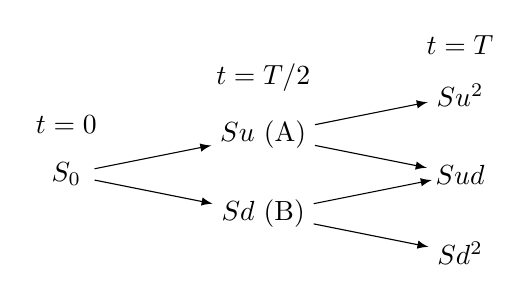
\begin{tikzpicture}[
                   grow = right,
edge from parent/.style = {draw,-latex},
         label distance = 1.5mm,
      every node/.style = {minimum width=2em, inner sep=3pt},
         level distance = 25mm,
       sibling distance = 10mm,
                     ]
\node[label=90:{$t=0$}] {$S_0$}
    child {node {$Sd$ (B)}
        child {node {$Sd^2$}
            %child {node {40}}
            %child {node {20}}
                }
        child {node {}}%<---------------- already printed
            }
    child {node[label=90:{$t=T/2$}] {$Su$ (A)}
        child {node {$Sud$}
            %child {node {}}%<------------ already printed
            %child {node {0}}
                }
        child {node[label=90:{$t=T$}] {$Su^2$}
            %child {node {}}%<------------ already printed
            %child {node[label=90:{$t=3$}] {0}}
                }
                };
\end{tikzpicture}
\end{center}
and focus on node (A). We have two different interest rates, $R_{\nicefrac{T}{2}}=R(0,\nicefrac{T}{2})$ and $R_T=R(0,T)$, called \emph{spot interest rates} because they start from $t=0$. The problem is to compute $q$: we would like to find an expression similar to \eqref{qT2} but we need $R=R(0,\nicefrac{T}{2},T)$ -- i.e. the interest rate decided at $t=0$ that starts to capitalize at $t=\nicefrac{T}{2}$ until $t=T$ -- which is not defined yet. $R=R(0,\nicefrac{T}{2},T)$ is called \emph{forward interest rate}. We would like to deduce the value of the forward interest rate starting from the spot interest rates. If we put \EUR{1} at $t=0$ we have
\begin{equation*}
    1 \longrightarrow e^{R\left(0,\frac{T}{2}\right)\frac{T}{2}} \longrightarrow e^{R\left(0,\frac{T}{2}\right)\frac{T}{2}}e^{R\left(0,\frac{T}{2},T\right)\frac{T}{2}}
\end{equation*}
which has to be consistent with the one shot capitalization using
\begin{equation*}
    1\longrightarrow e^{R(0,T)T}
\end{equation*}
otherwise there is an arbitrage opportunity. We obtain the following equation:
\begin{equation}\label{equality}
    e^{R\left(0,\frac{T}{2}\right)\frac{T}{2}}e^{R\left(0,\frac{T}{2},T\right)\frac{T}{2}} = e^{R(0,T)T}
\end{equation}
which has solution
\begin{equation}
    R\left(0,\frac{T}{2},T\right) = \dfrac{R(0,T)T + R\left(0,\frac{T}{2}\right)\frac{T}{2}}{\frac{T}{2}}
\end{equation}
Now we can define the risk neutral probability in the node (A):
\begin{equation}
    q_A = \dfrac{e^{R\left(0,\frac{T}{2},T\right)\frac{T}{2}}-d}{u-d}
\end{equation}
The same argument holds for node (B), so the expression for $q_B$ is exactly the same of $q_A$. The interest rate at $t=0$ will be
\begin{equation}
    q_0 = \dfrac{e^{R\left(0,\frac{T}{2}\right)\frac{T}{2}}-d}{u-d}
\end{equation}
So, denoting $q_A = q_B \equiv q_1$, the price at $t=0$ is given by
\begin{equation}\label{p00}
    price_0
    \left(
    \begin{matrix}
        f^{u^2} \\ f^{ud} \\ f^{d^2}
    \end{matrix}
    \right)
    = e^{-R(0,T)T} \mathbb{E}^{\Qmeas}[\mbox{payoff}_T]
\end{equation}
where
\begin{equation}
    Q \sim \left(
    \begin{matrix}
        q_0q_1 \\ q_0(1-q_1)+(1-q_0)q_1 \\ (1-q_0)(1-q_1)
    \end{matrix}
    \right)
\end{equation}
Expanding \eqref{p00} we get
\begin{equation}
    price_0
    \left(
    \begin{matrix}
        f^{u^2} \\ f^{ud} \\ f^{d^2}
    \end{matrix}
    \right)
    = e^{-R(0,T)T}(f^{u^2}q_0q_1 + f^{ud}(q_0(1-q_1)+(1-q_0)q_1) + f^{d^2}(1-q_0)(1-q_1))
\end{equation}

\subsection{Binary call at the money}\lesson{5}{19/03/2020}
We consider, as an example, the binary call at the money. In this case, the payoff is 
\begin{equation}
    \mbox{payoff}_T = \mathds{1}_{S_T\ge K}
\end{equation}
and $K=S_0$ (at the money). So, when it is possible to exercise the contract, the cash flow is always equal to 1. Consider a toy model with $u=1.1$, $d=0.9$ and $S_0=K=100$:
\begin{center}
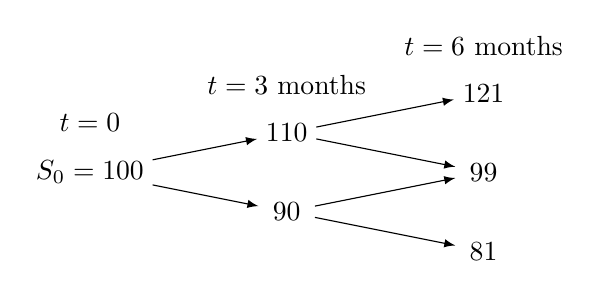
\begin{tikzpicture}[
                   grow = right,
edge from parent/.style = {draw,-latex},
         label distance = 1.5mm,
      every node/.style = {minimum width=2em, inner sep=3pt},
         level distance = 25mm,
       sibling distance = 10mm,
                     ]
\node[label=90:{$t=0$}] {$S_0=100$}
    child {node {90}
        child {node {81}
            %child {node {40}}
            %child {node {20}}
                }
        child {node {}}%<---------------- already printed
            }
    child {node[label=90:{$t=3$ months}] {110}
        child {node {99}
            %child {node {}}%<------------ already printed
            %child {node {0}}
                }
        child {node[label=90:{$t=6$ months}] {121}
            %child {node {}}%<------------ already printed
            %child {node[label=90:{$t=3$}] {0}}
                }
                };
\end{tikzpicture}
\end{center}
The payoff is 
\begin{equation}
    \mbox{payoff}_T = 
    \left( 
    \begin{matrix}
    1 \\ 0 \\ 0
    \end{matrix}
    \right)
\end{equation}
We would like to price this option. The input are the zero coupon bonds at these maturities:
\begin{enumerate}
    \item The first has notional value 1 at 3 months and 
    its price today is 1.001. 
    \begin{equation*}
        1.001 = e^{-R(0,3m)\frac{3}{12}}\cdot1 \qquad\Rightarrow\qquad R(0,3m) = -0.001 = -0.1\%
    \end{equation*}
    This means that the interest rate is negative and it is as if we pay in order to keep our money safe.
    \item The second has notional value 1 at 6 months an its price today is 1, so the interest rate is zero.
\end{enumerate}
In order to find which is the forward interest rate, we use eq. \eqref{equality}:
\begin{equation}\label{equality1}
    e^{R\left(0,3m\right)\frac{3}{12}}e^{R\left(0,3m,6m\right)\frac{3}{12}} = e^{R(0,6m)\frac{6}{12}}
\end{equation}
which has solution
\begin{equation}
    R\left(0,3m,6m\right) = 2\underbrace{R(0,6m)}_{=0}-R\left(0,3m\right) = 0.1\%
\end{equation}
Therefore, the risk neutral probability weights are given by
\begin{equation}
    q_1 = \dfrac{e^{R\left(0,3m,6m\right)\frac{3}{12}}-d}{u-d} = 4.501, \qquad q_0 = \dfrac{e^{R\left(0,3m\right)\frac{3}{12}}-d}{u-d} = 4.499
\end{equation}
Now we are able to price the corresponding binary option:
\begin{equation}
    price_0^{BinCall} = e^{-RT}\mathbb{E}^{\Qmeas}[\mbox{payoff}_T] = e^{-RT}\mathbb{E}^{\Qmeas}\left[
    \left( 
    \begin{matrix}
    1 \\ 0 \\ 0
    \end{matrix}
    \right)
    \right]
\end{equation}
where
\begin{equation}
    Q \sim \left(
    \begin{matrix}
    q_0q_1 \\ (1-q_0)q_1+q_0(1-q_1) \\ (1-q_0)(1-q_1)
    \end{matrix}
    \right)
\end{equation}
which gives
\begin{align}
    \notag price_0^{BinCall} 
    &= 
    \notag e^{-R(0,6m)\frac{6}{12}}(1\cdot q_0q_1 + 0\cdot (1-q_0)q_1+q_0(1-q_1) + 0\cdot (1-q_0)(1-q_1)) \\
    &=
    e^{-R(0,6m)\frac{6}{12}}q_0q_1
\end{align}
For the hedging the story is the same. \colorbox{cyan}{scrivi}

\section{General binomial model}
Now we consider a generic number of time steps, so that the underlying is $S_T\in\mathbb{R}^{t+1}$ and has terminal value
\begin{equation}
    \left(
    \begin{matrix}
    Su^t \\ Su^{t-1}d \\ \vdots \\ Su^jd^{t-j} \\ \vdots \\ Sud^{t-1} \\ Sd^t
    \end{matrix}
    \right)
\end{equation}
where $j$ represents the number of up moves in the lattice. The payoff (for the call option) we want to compute is 
\begin{equation}
    \mbox{payoff}_T = (S_T-K)^+
\end{equation}
Then the value of the corresponding replicating portfolio is
\begin{align}
    \notag P_t(j) 
    &=
    \notag V_t(j) \overset{(a)}{=} e^{-R\cdot1}(qV_{t+1}(j+1) + (1-q)V_{t+1}(j)) \\
    &=
    e^{-R}\mathbb{E}^{\Qmeas}[V_{t+1}|j]
\end{align}
% forse ha usato V per indicare "value", ma crea confusione quindi forse è meglio usare sempre P
where in (a) we used the backward induction procedure using unitary time steps and constant $q=\frac{e^R-d}{u-d}$. At the end, the corresponding value is
\begin{equation}
    P_T(j) = (S_0u^jd^{T-j}-K)^+
\end{equation}
Considering the hedging, we have
\begin{equation}
    \Delta_t(j)=\dfrac{V_{t+1}(j+1)-V_{t+1}(j)}{S_tu-S_td}, \qquad \beta_t(j)=e^{-Rt}(V_t(j)-\Delta_t(j)S_t) 
\end{equation}
So the initial price can be written as:
\begin{equation}
    p_0(call)=e^{-RT}\sum^{T}_{j=0}\binom{T}{j}q^j(1-q)^{T-j}(Su^j d^{T-j}-K)^+
\end{equation}
\begin{remark}
    Notice that the probability distribution
    \begin{equation}
        Q \sim \left(
        \begin{matrix}
        q^T \\ \vdots \\ \binom{T}{j}q^j(1-q)^{T-j} \\ \vdots \\ (1-q)^T
        \end{matrix}
        \right)
    \end{equation}
    is normalized, in fact
    \begin{equation}
        \sum^{T}_{j=0}\binom{T}{j}q^j(1-q)^{T-j} = (q+1-q)^T = 1
    \end{equation}
    where we used the fact that $(a+b)^n=\sum^{n}_{j=0}\binom{n}{j}q^j(1-q)^{n-j}$.
\end{remark}


\section[Convergence of the binomial model]{From the binamial model to a geometric brownian motion}
Now we want to see if the binomial model leads to convergence if we take a number of steps which tends to infinity. Let's consider a binomial model with unitary time steps, $n<T$ and $T=m$. The underlying at time $n+1$ is defined as
\begin{equation}\label{Sn+1}
    S_{n+1} = S_nZ_{n+1}
\end{equation}
where $Z_n$ are i.i.d. random variables with binomial distribution and risk neutral probability
\begin{equation}
    Q(Z_{n+1}=u_n)=q_n, \qquad Q(Z_{n+1}=d_n)=1-q_n
\end{equation}
with 
\begin{equation}
    q_n = \dfrac{e^R-d_n}{u_n-d_n}
\end{equation}
In principle, if we consider this particular binomial model and we consider the discounted asset $S_ne^{-Rn}$, it turn out to be a $Q$-martingale, i.e. a martingale under the measure ${\Qmeas}$. This means that $S_ne^{-Rn}$ is constant in expected value and that
\begin{equation}
    \mathbb{E}^{\Qmeas}[Z_n] = e^{R\frac{T}{n}}
\end{equation}
In order to prove it, it is sufficient to start from eq. \eqref{Sn+1} \colorbox{cyan}{to do (6:50)}.\\
We would like to shift from the multiplicative structure of \eqref{Sn+1} to an additive structure. This can be done just by taking the logarithm of eq. \eqref{Sn+1}:
\begin{equation}\label{lnSn}
    \ln S_n = \ln S_0 + \sum_{i=1}^n\ln Z_i
\end{equation}
The sum in \eqref{lnSn} is a sum of bounded i.i.d random values, so we can use the Central Limit Theorem in order to show that it converges to a gaussian random variable. However, the convergence is not well defined as $\low(\ln Z_i)$ depends on $n$ and when the random variable depends on the number of random variables considered we have to be careful in considering the limit. So we can not use a simple version of the CLT. The idea is to show that 
\begin{equation}
    \low(S_n)\to\low(S_T)
\end{equation}
where $S_T$ is the terminal value of a process $S_t$ satisfying
\begin{equation}\label{geom_brow}
    \dv{S_t}{t} = r\dd t + \sigma\dd W^{\Qmeas}_t
\end{equation}
where $W^{\Qmeas}_t$ is a brownian motion under the probability measure ${\Qmeas}$. In order to study the convergence it is better to work with the corresponding characteristic function, which is the Fourier transform of the pdf:
\begin{align}\label{phi111}
    \notag \phi_{\ln S_n}(\lambda)
    &=
    \mathbb{E}^{\Qmeas}[e^{i\lambda\ln S_n}] \overset{\eqref{lnSn}}{=} e^{i\lambda\ln S_0}\left(\mathbb{E}^{\Qmeas}\left[e^{i\lambda\ln Z}\right]\right)^n \\
    &= S_0^{i\lambda}\left(qe^{i\lambda\ln n}+(1-q)e^{i\lambda\ln d}\right)^n
\end{align}
Now we define the relation between $(u,d)$ and $(r,\sigma)$. Let's take
\begin{equation}\label{undn}
    u_n=e^{\sigma\sqrt{\frac{T}{n}}}, \qquad d_n=e^{-\sigma\sqrt{\frac{T}{n}}}
\end{equation}
which is in line with what we did in sec. \ref{sec:impl}. Now we have to link the interest rate for the period in the binomial model with the corresponding interest rate in the continuous time version:
\begin{equation}\label{Rr}
    e^R = e^{r\frac{T}{n}}
\end{equation}
where $R$ is the discrete time interest rate and $r$ is the continuous time interest rate. Plugging this mapping in \eqref{phi111} we get:
\begin{align}\label{phi222}
    \notag \phi_{\ln S_n}(\lambda) 
    &=
    S_0^{i\lambda}\left(qe^{i\lambda\sigma\sqrt{\frac{T}{n}}}+(1-q)e^{-i\lambda\sigma\sqrt{\frac{T}{n}}}\right)^n \\
    &\overset{(a)}{=}
    \notag S_0^{i\lambda}\left[q
    \left(
    1+i\lambda\sigma\sqrt{\frac{T}{n}}-\frac{1}{2}\lambda^2\sigma^2\frac{T}{n}+\order{n^{-1}}
    \right) + \right. \\
    &\notag\qquad
    \left.+(1-q)\left(
    1-i\lambda\sigma\sqrt{\frac{T}{n}}-\frac{1}{2}\lambda^2\sigma^2\frac{T}{n}+\order{n^{-1}}
    \right)
    \right]^n \\
    &= 
    S_0^{i\lambda}\left(1+i\lambda\sigma\sqrt{\frac{T}{n}}(2q-1)-\frac{1}{2}\lambda^2\sigma^2\frac{T}{n}+\order{n^{-1}}\right)^n
\end{align}
where in (a) we used the Taylor expansion. Now, recall that $q = \frac{e^R-d}{u-d}$, so using \eqref{undn}, \eqref{Rr} and Taylor expanding we get
\begin{align}
    \notag q 
    &=
    \dfrac{e^{r\frac{T}{n}}-e^{-\sigma\sqrt{\frac{T}{n}}}}{e^{\sigma\sqrt{\frac{T}{n}}}-e^{-\sigma\sqrt{\frac{T}{n}}}} \\
    &= 
    \notag \dfrac{1+r\frac{T}{n}-1+\sigma\sqrt{\frac{T}{n}}-\frac{1}{2}\sigma^2\frac{T}{n}+\order{n^{-1}}}{1+\sigma\sqrt{\frac{T}{n}}+\frac{1}{2}\sigma^2\frac{T}{n}-1+\sigma\sqrt{\frac{T}{n}}-\frac{1}{2}\sigma^2\frac{T}{n}+\order{n^{-1}}} \\
    &=
    \notag \dfrac{\sigma+\left(r-\frac{\sigma^2}{2}\right)\sqrt{\frac{T}{n}}+\order{n^{-1/2}}}{2\sigma+\order{n^{-1/2}}} \\
    &=
    \frac{1}{2}+\dfrac{1}{2\sigma}\left(r-\frac{\sigma^2}{2}\right)\sqrt{\frac{T}{n}}+\order{n^{-1/2}}
\end{align}
Then we have
\begin{equation}
    2q-1 = \dfrac{1}{\sigma}\left(r-\frac{\sigma^2}{2}\right)\sqrt{\frac{T}{n}}+\order{n^{-1/2}}
\end{equation}
and we can plut it into \eqref{phi222}:
\begin{align}\label{phi333}
    \notag \phi_{\ln S_n}(\lambda) 
    &=
    \notag S_0^{i\lambda}\left(1+i\lambda\cancel{\sigma}\left(r-\frac{\sigma^2}{2}\right)\cancel{\frac{1}{\sigma}}\frac{T}{n}-\frac{1}{2}\lambda^2\sigma^2\frac{T}{n}+\order{n^{-1}}\right)^n \\
    &= 
    S_0^{i\lambda}\left[1+\frac{1}{n}\left(
    i\lambda T\left(r-\frac{\sigma^2}{2}\right)-\frac{1}{2}\lambda^2\sigma^2 T\right)\right]^n
\end{align}
Recall that 
\begin{equation*}
    \lim_{n\to+\infty}\left(1+\dfrac{a}{n}\right)^n = e^a
\end{equation*}
so if in \eqref{phi333} we define $a = \left(i\lambda T\left(r-\frac{\sigma^2}{2}\right)-\frac{1}{2}\lambda^2\sigma^2 T\right)$, we have that 
\begin{equation}\label{lim_phi}
    \lim_{n\to+\infty} \phi_{\ln S_n}(\lambda) = S_0^{i\lambda}\exp\left[i\lambda T \left(r-\frac{\sigma^2}{2}\right)-\frac{1}{2}\lambda^2\sigma^2 T \right]
\end{equation} 
Now we have to understand how \eqref{lim_phi} is related to the characteristic function of the terminal value of $\ln S_T$ in the continuous time framework, $\mathbb{E}^{\Qmeas}\left[e^{i\lambda\ln S_T}\right]$. We will find that the solution of \eqref{geom_brow} is 
\begin{equation}
    S_T = S_0e^{\left(r-\frac{\sigma^2}{2}\right)T+\sigma W_T^{\Qmeas}}
\end{equation}
$W_T^{\Qmeas} \sim \mathcal{N}(0;T)$ so the brownian motion has a gaussian distribution with variance equal to the time window we are considering. This means that $S_T$ is a random variable distributed as 
\begin{equation}\label{ST}
    S_T\sim S_0\exp\left[\underbrace{\ln S_0+\left(r-\frac{\sigma^2}{2}\right)T}_{deterministic}+\underbrace{\sigma\mathcal{N}(0;T)}_{stochastic}\right]
\end{equation}
The deterministic part represents just a shift in the expected value, so we can rewrite \eqref{ST} as
\begin{equation}
    S_T\sim S_0\exp[\sigma\mathcal{N}\left(\ln S_0+\left(r-\frac{\sigma^2}{2}\right)T;\sigma^2 T\right)]
\end{equation}
So $S_T$ follows a log-normal distribution. Now recall the characteristic function of a gaussian variable
\begin{equation}
    \mathbb{E}^{\Qmeas}\left[e^{i\lambda\mathcal{N}(\mu;\sigma^2)}\right] = e^{i\lambda\mu-\frac{\sigma^2\lambda^2}{2}}
\end{equation}
In our case we have:
\begin{align}
    \mathbb{E}^{\Qmeas}\left[e^{i\lambda\ln S_T}\right] 
    &=
    \mathbb{E}^{\Qmeas}\left[e^{i\lambda\mathcal{N}\left(\ln S_0+\left(r-\frac{\sigma^2}{2}\right)T;\sigma^2 T\right)}\right] \\
    &=
    \exp\left(i\lambda\ln S_0+i\lambda\left(r-\frac{\sigma^2}{2}\right)T-\dfrac{\sigma^2\lambda^2}{2}T\right) \\
    &=
    S_0^{i\lambda}\exp\left(i\lambda\left(r-\frac{\sigma^2}{2}\right)T-\dfrac{\sigma^2\lambda^2}{2}T\right)
\end{align}
This is the characteristic function of the geometric brownian motion. Going back to \eqref{lim_phi} we find exactly the same expression, so the binomial model converges to the characteristic function of the corresponding solution of the geometric brownian motion.
\subsection[The Black \& Scholes formula]{Call option price in binomial model: the Black \& Scholes formula}\lesson{6}{20/03/2020}
The call option price in a $n$ steps binomial model is given by the one shot discounted value of the risk neutral expectation of the payoff:
\begin{equation}\label{pr0}
    p_0(call)=e^{-RT}\sum^{n}_{j=0}\binom{n}{j}q^j(1-q)^{n-j}(Su^j d^{n-j}-K)^+
\end{equation}
We would like to remove the non-linearity in the positive part. In order to do that we have to find when $(Su^j d^{n-j}-K)^+\ge0$, so that we can remove the positive part. So we look for the smallest index $j$ such that $(Su^j d^{n-j}-K)^+\ge0$:
\begin{equation}
    \hat{\jmath} = \inf\{j:S_0u^2d^{n-j}\ge K\}
\end{equation}
Taking the logarithm of $S_0u^2d^{n-j}\ge K$ we get:
\begin{equation}
    \ln S_0 + j\ln n + (n-j)\ln d \ge \ln K
\end{equation}
\begin{equation}
    j(\ln n - \ln d) \ge \ln\dfrac{K}{S_0}-n\ln d
\end{equation}
\begin{equation}\label{jhat}
    \hat{\jmath} = \floor*{\dfrac{\ln\frac{K}{S_0}-n\ln d}{\ln n - \ln d}} \overset{\eqref{undn}}{=} \floor*{\dfrac{\ln\frac{K}{S_0}+n\sigma\sqrt{\frac{T}{n}}}{2\sigma\sqrt{\frac{T}{n}}}}=
    \floor*{\dfrac{n}{2}-\dfrac{\ln\frac{S_0}{K}}{2\sigma\sqrt{\frac{T}{n}}}}
\end{equation}
Now we can rewrite \eqref{pr0} as:
\begin{align}\label{pr01}
    \notag p_0(call)
    &=
    e^{-RT}\sum^{n}_{j=\hat{\jmath}}\binom{n}{j}q^j(1-q)^{n-j}Su^j d^{n-j}- Ke^{-RT}\sum^{n}_{j=\hat{\jmath}}\binom{n}{j}q^j(1-q)^{n-j}\\
    &=
    S\sum^{n}_{j=\hat{\jmath}}\binom{n}{j}\left(e^{-\frac{RT}{n}}qu\right)^j\left(e^{-\frac{RT}{n}}(1-q)d\right)^{n-j} - Ke^{-RT}\sum^{n}_{j=\hat{\jmath}}\binom{n}{j}q^j(1-q)^{n-j}
\end{align}
where we took $S$ out of the sum, $e^{RT}$ inside it and split the resulting sum in two components. Notice that
\begin{equation*}
    e^{-\frac{RT}{n}}qu + e^{-\frac{RT}{n}}(1-q)d=1, \qquad\Rightarrow\qquad q + 1-q = 1
\end{equation*}
so we can interpret them as probability weights. In particular we can see them as the expansion of the binomial distribution, in fact the cumulated risk neutral probability of a binomial random variable parametrized by $p$ and $n$ is\footnote{Recall that a binomial random variable is the sum of $n$ Bernoulli independent random variables with parameter $p$.}
\begin{equation}
    Q(\mathcal{B}(p,n)\ge a) = \sum_{j=n}^a\binom{n}{j}p^j(1-p)^{n-j}
\end{equation}
and the terms in eq. \eqref{pr01} have the same structure. So we get the intuition that applying carefully the CLT we can say that
\begin{equation}
    e^{-\frac{RT}{n}}qu \ovun{\longrightarrow}{``CLT"}{n\to\infty}\mathcal{N}(ne^{-\frac{RT}{n}}qu;ne^{-\frac{RT}{n}}qu(1-e^{-\frac{RT}{n}}qn))
\end{equation}
\begin{equation}
    e^{-\frac{RT}{n}}(1-q)d \ovun{\longrightarrow}{``CLT"}{n\to\infty} \mathcal{N}(nq;nq(1-q))
\end{equation}
Now \eqref{pr01} becomes
\begin{equation}\label{pr02}
    p_0(call) = SQ(\mathcal{B}(e^{-\frac{RT}{n}}qu;n)\ge\hat{\jmath})-KQ(\mathcal{B}(q;n)\ge\hat{\jmath})
\end{equation}
This is the so called \emph{Black \& Scholes forumula}. Then we consider the second part. Recall that
\begin{align}
    \notag \prob(\mathcal{N}(\mu,\sigma^2)>\hat{\jmath})
    &=
    \prob\left(\mathcal{N}(0,1)>\dfrac{\hat{\jmath}-\mu}{\sigma}\right) \\
    &\overset{(a)}{=} \notag \prob\left(\mathcal{N}(0,1)<\dfrac{\mu-\hat{\jmath}}{\sigma}\right) \\
    &\overset{(b)}{=} \Phi\left(\dfrac{\mu-\hat{\jmath}}{\sigma}\right)
\end{align}
where in (a) we used the symmetry of the standardized gaussian and in (b) we recognized the \emph{cumulative probability function}
\begin{equation}
\Phi(x)=\int^{x}_{-\infty}\frac{1}{\sqrt{2\pi}}e^{-\frac{z^2}{2}}\,\dd z
\end{equation}
In our case $\mu=nq$ and $\sigma=\sqrt{nq(1-q)}$, so we get:
\begin{align}
    \notag\Phi\left(\dfrac{nq-\hat{\jmath}}{\sqrt{nq(1-q)}}\right)
    &= \Phi\left(\left(nq-\dfrac{n}{2}-\dfrac{\ln\frac{S_0}{K}}{2\sigma\sqrt{\frac{T}{n}}}\right)\dfrac{1}{\sqrt{nq(1-q)}}\right) \\
    &=
    \notag\Phi\left(
    \dfrac{\sqrt{n}\left(q-\frac{1}{2}\right)}{\sqrt{q(1-q)}} + \dfrac{\ln\frac{S_0}{K}}{2\sigma\sqrt{T}\sqrt{q(1-q)}}
    \right)\\
    &=
    \Phi\left(
    \dfrac{\ln\frac{S_0}{K}+\left(r-\frac{\sigma^2}{2}\right)T}{\sigma\sqrt{T}}
    \right)
\end{align}
where in the first step we used the definiton of $\hat{\jmath}$ \eqref{jhat} and in the last we used the following limits:
\begin{align}\label{lim}
    q(1-q)\overset{n\to\infty}{\longrightarrow}\frac{1}{4}, \qquad
    \sqrt{n}\left(q-\frac{1}{2}\right) \overset{n\to\infty}{\longrightarrow}\frac{\left(r-\frac{\sigma}{2}\sqrt{T}\right)}{2\sigma}
\end{align}
\colorbox{cyan}{dimostra.} So the gaussian cumulative probability function can be written in terms of the continuous time variables. The same argument holds for the the first term of \eqref{pr01}, so that with this limit procedure we recovered the Black \& Scholes formula \eqref{pr02}.\\
This is just an intuition in order to understand that not only the underlying but also the call option price is quite robust in this procedure. So the binomial model approximates very well the continuous time pricing model and this is the reason why nowadays this model is widely used in the banking industry.\\
We will came back to the Black \& Scholes formula after introducing the stochastic calculus in continuous time.

\section{American options} %vedi libro per riscrivere meglio
So far we considered the cases in which the payoff was $(S_T-K)^+$ and in which we can exercise the option to buy/sell only at the maturity. These options are called \emph{European options}. On the contrary, in \emph{American options} we can exercise the option -- i.e. the possibility -- at any time $t\le T$. It is now obvious to compute the payoff $(S_{\tau}-K)^+$ in American options, since we don't know the time $\tau$ at which we will be interested to exercise. So, in order to compute the initial price of an American call we need an information involving future time, which is not measurable. The time $\tau$ is a random variable called \emph{stopping time}.

\subsection{Call option with no dividends and \texorpdfstring{$R>0$}{R>0}}
Now, consider a special case in which we have a call option on a non-dividend paying. In this case the American call price at any time $t$ will be always greater than the price of an European contract:
\begin{equation*}
    C^{AM}(t,S_t)\ge C^{EU}(t,S_t)
\end{equation*}
because the American option includes the opportunity to exercise at the end but also at any time $t$, so it is better than the European one. Furthermore, we have that
\begin{equation*}
    C^{AM}(t,S_t) \ge S_t - Ke^{-R(T-t)}
\end{equation*}
This is due to the absence of an arbitrage opportunity. In fact, if we consider a long call we buy the call option at price $C_t$ and at the end we get the corresponding payoff $(S_T-K)^+$. Then we go short today, receiving the corresponding market price $S_t$ and engaging ourselves to re-buy at the end at price $-S_T$. Finally we go long on the riskless asset investing $Ke^{-R(T-t)}$ and getting $K$ at the end.
\begin{center}
    \begin{tabular}{lcc}\toprule
        Action & $t=0$ & $t=T$ \\\midrule
        Long call & $-C_t$ & $(S_T-K)^+$ \\
        Sell short & $+S_t$ & $-S_T$ \\
        Invest in the riskless market & $-Ke^{-R(T-t)}$ & $+K$ \\ \midrule\midrule
         & $S_t-C_t-Ke^{-RT}$ & $(S_T-K)^+-(S_T-K)\ge 0$ \\\bottomrule
    \end{tabular}
\end{center}
In order to avoid an arbitrage opportunity it must be:
\begin{equation*}
    S_t-C_t-Ke^{-RT} \le 0 \qquad\Rightarrow\qquad C^{AM}(t,S_t)\ge S_t-Ke^{-RT}
\end{equation*}
Of course, if the interest rate is positive -- which is not always the case -- then
\begin{equation*}
    C^{AM}(t,S_t) \ge S_t - K \qquad\forall t<T
\end{equation*}
Since $C^{AM}(t,S_t)\ge0$, then
\begin{equation*}
    C^{AM}(t,S_t)\ge \max(0,S_t-K)=(S_t-K)^+
\end{equation*}
This means that if there are no dividends and the interest rate is positive it is always better to wait because what we get if we decide to exercise today is always less than the value of the American option. In other words, in this case the European option is better, so there will be no differences between American and European options:
\begin{equation*}
    C^{AM}(t,S_t)=C^{EU}(t,S_t)
\end{equation*}

\subsection{General discrete time case with no dividends and \texorpdfstring{$R=0$}{R=0}}
% subsection o section?
% Bjork ch. 21 or Lamberton
Now we consider the general discrete time case with no dividends and $R=0$. Let's start with some definitions.
\begin{definition}[Stopping time]
A non-negative random variable $\tau$ is called \emph{(optional) stopping time} with respect to the \emph{filtration}\footnote{A family $\{G_t:t\ge0\}$ of sub-$\sigma$-algebras is called a \emph{filtration} if $s < t$ implies $G_s \subseteq G_t$.} $\mathcal{F}$ if
\begin{equation}
    \{\tau \le n\}\in\mathcal{F}_n \qquad\forall n\ge0
\end{equation}
Since we are considering a discret time framework, this is equivalent to
\begin{equation}
    \{\tau \le n\}\in\mathcal{F}_n \qquad\forall n\ge0
\end{equation}
\end{definition}
\noindent So if a random variable is a stopping time we are able to state that the event $\tau\le n$ is true or false on the basis of the information available at time $n$. This means that $\tau$ is a \emph{non-anticipative} random value.
\begin{definition}[Optimal stopping time]
Given a real number $T<\infty$, consider a family $Z_n\in L^1$ of random variables. If $\hat{\tau}$ is a stopping time such that
\begin{equation}
    \sup_{0\le\tau\le T}\mathbb{E}[Z_{\tau}] = \mathbb{E} [Z_{\hat{\tau}}]
\end{equation}
then $\hat{\tau}$ is called \emph{optimal stopping time}.
\end{definition}
\noindent Now we ask ourselves: does $\hat{\tau}$ exist? Is $\hat{\tau}$ unique? Even if $\hat{\tau}$ exists and is unique, how can we compute it? We try to answer these questions using a preliminary result.
\begin{proposition}\label{martingales}
Consider a random variable $Z$ and $T<\infty$.
\begin{enumerate}
    \item If $Z$ is a sub-martingale, i.e. its expected value increases in time, then $\hat{\tau}=T$.
    \item If $Z$ is a super-martingale, i.e. its expected value decreases in time, then $\hat{\tau}=0$.
    \item If $Z$ is a martingale, i.e. its expected value is constant in time, then all times $\tau$ are optimal.
\end{enumerate}
\end{proposition}
\begin{definition}[Value process]
Fix $n\le T$ and consider a stopping time $n\le\tau\le T$. The \emph{value process} is defined as
\begin{equation}
    J_n(\tau) \coloneqq \mathbb{E}[Z_{\tau}|\mathcal{F}_n]
\end{equation}
and the \emph{optimal value process} is
\begin{equation}\label{Vn}
    V_n \coloneqq \ess\sup_{0\le\tau\le T} \mathbb{E}[Z_{\tau}|\mathcal{F}_n]
\end{equation}
\end{definition}
\noindent In eq. \eqref{Vn} we are taking the essential supremum, which intuitively is the value that is larger or equal than the function values everywhere when allowing for ignoring what the function does at a set of points of measure zero.
\begin{definition}
The \emph{optimal stopping time} at time $n$ is $\hat{\tau}_n$ such that $V_n=V_{\hat{\tau}_n}$.
\end{definition}
\begin{example}{}{}
Consider
\begin{equation*}
    f(x)=\begin{cases}
    5 & x=1 \\
    -4 & x=-1 \\
    2 & \mbox{otherwise}
    \end{cases}
\end{equation*}
In this case $\sup f(x)=5$ and $\inf f(x)=-4$, but notice that they are points of zero measure (with respect to the Lebesgue measure), since the function is almost everywhere equal to 2. So, in this case
\begin{equation*}
    \ess\sup f(x) = \ess\inf f(x) = 2
\end{equation*}
\end{example}
\begin{example}{}{}
Consider
\begin{equation*}
    f(x)=\begin{cases}
    \frac{1}{x} & x\in\mathbb{Q}\setminus\{0\} \\
    0 & x=0 \\
    2 & x\in\mathbb{R}\setminus\mathbb{Q}
    \end{cases}
\end{equation*}
In this case $\sup f(x)=\infty$ but $\ess\sup f(x)=0$ since the Lebesgue measure of the set of rational points is zero.
\end{example}

\subsection{Possible strategies at time \texorpdfstring{$n$}{n}}\lesson{7}{25/03/2020}
We want to study which are the possible strategies to use at time $n$, dealing with American options. Essentially, we have three possibilities:
\begin{enumerate}
    \item Use $\hat{\tau}_n$ and get the corresponding optimal value process $V_n$;
    \item Stop now, getting the corresponding payoff $Z_n$;
    \item Wait untill $n+1$ and adopt the corresponding stopping time $\hat{\tau}_n$, getting nothing at time $n$ and $Z_{\hat{\tau}_{n+1}}$ at time $n+1$. According to the neutral risk methodology, the value of $Z_{\hat{\tau}_{n+1}}$ at time $n$ is given by 
    \begin{equation}
        \mathbb{E}^{\Qmeas}[Z_{\hat{\tau}_{n+1}}\mid\mathcal{F}_n] \overset{(a)}{=} \mathbb{E}^{\Qmeas}[\mathbb{E}^{\Qmeas}[Z_{\hat{\tau}_{n+1}}\mid\mathcal{F}_{n+1}]\mid\mathcal{F}_n] = \mathbb{E}^{\Qmeas}[V_{n+1}\mid\mathcal{F}_{n+1}]\mid\mathcal{F}_n]
    \end{equation}
    where in (a) we used the so called tower property of the conditional expected value\footnote{The tower property of the conditional expected value states that if $\mathcal{F}_{1}\subset\cdots \subset\mathcal{F}_{n}\subset\mathcal{F}_{m}\subset\cdots\subset\mathcal{F}_{N}$ is a family of sub-$\sigma$-algebras, we have $E[X\mid\mathcal{F}_{n}] = E[E[X\mid \mathcal{F}_{n+m}]\mid\mathcal{F}_{n}]$.}. So the market value at time $n$ is given by the conditional expected value up to the current available information $\mathcal{F}_n$ of what will become optimal at time $n+1$
\end{enumerate}
Since option 1 is optimal, it is better than options 2 and 3:
\begin{equation}\label{Vndis}
    \begin{cases}
    V_n \ge Z_n \\
    V_n \ge \mathbb{E}^{\Qmeas}[V_{n+1}\mid\mathcal{F}_{n}]
    \end{cases}
\end{equation}
This represents a simple control problem in which we have only two possibilities at time $n$: stop or wait.
\begin{itemize}
    \item If we stop it means that it is optimal to stop, so $\hat{\tau}_n=n$ and $V_n=Z_n$;
    \item If we wait it means that it is not optimal to stop, so $\hat{\tau}_n=\hat{\tau}_{n+1}$ and $V_n=\mathbb{E}^{\Qmeas}[V_{n+1}\mid\mathcal{F}_{n}]$
\end{itemize}
According to these possibilities we can characterize the \emph{optimal rule}, which maximizes them.
\begin{theorem}
\hfill
\begin{enumerate}[i.]
    \item The optimal value process $V$ solves the \emph{backward equation}
    \begin{equation}
        \begin{cases}
        V_n = \max\{Z_n,\mathbb{E}^{\Qmeas}[V_{n+1}\mid\mathcal{F}_{n}]\}\\
        V_T = Z_T = \mbox{payoff}_T
        \end{cases}
    \end{equation}
    \item $\hat{\tau}_{n}=n \Leftrightarrow V_n=Z_n$;
    \item If $\hat{\tau}>n$ then $V_n>Z_n$ and $V_n=\mathbb{E}^{\Qmeas}[V_{n+1}\mid\mathcal{F}_{n}]$.
\end{enumerate}
\end{theorem}
\begin{corollary}
\hfill
\begin{enumerate}[i.]
    \item The optimal stopping rule is given by $\hat{\tau}=\min\{n\ge0:V_n=Z_n\}$;
    \item For $n$ fixed, $\hat{\tau}_n=\min\{k\ge n:V_k=Z_k\}$;
\end{enumerate}
\end{corollary}

\subsection{Snell envelope}
Let $X$ and $Y$ be two adopted processes and let $\mathcal{F}_n$, $n\ge0$, be a given information structure.
\begin{definition}[Domination]
    $X$ \emph{dominates} $Y$ if $X_n\ge Y_n$ almost surely for all $n\ge0$.
\end{definition}
\begin{definition}[Snell envelope]
    If $Y\in L^1$, i.e. if $\mathbb{E}^{\Qmeas}[Y_n]<\infty$ $\forall n\le T$, the \emph{Snell envelope} of $Y$ is the smallest super-martingale dominating $Y$.
\end{definition}
\noindent So, the Snell envelope is the smallest super-martingale dominating a stochastic process. 
\begin{lemma}\label{lemma_snell}
    Let $\{D^{\alpha}\}_{\alpha\in A}$ be a family of super-martingales. Then $X_n\coloneqq\inf_{\alpha\in A}D_n^{\alpha}$ is a super-martingale.
\end{lemma}
\begin{proof}
    \begin{align*}
        \mathbb{E}^{\Qmeas}[X_{n+1}\mid\mathcal{F}_{n}] 
        &= 
        \mathbb{E}^{\Qmeas}[\inf_{\alpha\in A}D_{n+1}^{\alpha}\mid\mathcal{F}_{n}] \\
        &\le
        \inf_{\alpha\in A}\mathbb{E}^{\Qmeas}[D_{n+1}^{\alpha}\mid\mathcal{F}_{n}] \\
        &\le
        \inf_{\alpha\in A}D_{\bm{n}}^{\alpha} = X_n
    \end{align*}
    where the last inequality is true because $\{D^{\alpha}\}_{\alpha\in A}$ is a family of super-martingales.
\end{proof}
\begin{proposition}
    Consider a process $Y\in L^1$. Then there exists a Snell envelope of $Y$.
\end{proposition}
\begin{proof}
    If we take the family of super-martingales $\{D^{\alpha}\}_{\alpha\in A}$ dominating $Y$. Then $\forall n$
    \begin{equation*}
        D^{\alpha}_n \overset{a.s.}{\ge} Y_n
    \end{equation*}
    Now define $S_n\coloneqq\inf_{\alpha}D_n^{\alpha}$, which -- according to the lemma \eqref{lemma_snell} -- is a super-martingale and it is minimal. But $S_n$ dominates $Y$, so $S_n$ is a Snell envelope.
\end{proof}
\begin{theorem}[Snell envelope theorem]
    The optimal value process $V$ is the Snell envelope of the payoff process $Z$.
\end{theorem}
\begin{proof}
    From \eqref{Vndis} we have that $V_n$ is a super-martingale. Then we have to show that $V_n$ is minimal. Suppose that $X$ is a super-martingale dominating $Z$. Being X a super-martingale, we have that
    \begin{equation*}
        V_T=Z_T \quad\Rightarrow\quad X_T\ge Z_T = V_T, \qquad X_{n+1}\ge V_{n+1}
    \end{equation*}
    But for the same reason we also have 
    \begin{equation}\label{1}
        X_n \ge \mathbb{E}^{\Qmeas}[X_{n+1}\mid\mathcal{F}_n] \ge \mathbb{E}^{\Qmeas}[V_{n+1}\mid\mathcal{F}_n]
    \end{equation}
    $X$ dominates $Z$, so we have 
    \begin{equation}\label{2}
        X_n \ge Z_n
    \end{equation}
    Using \eqref{1} toghether with \eqref{2} we have that 
    \begin{equation*}
        X_n\ge \max\{Z_n,\mathbb{E}^{\Qmeas}[V_{n+1}\mid\mathcal{F}_n]\} \overset{def.}{=} V_n
    \end{equation*}
    So $X_n\ge V_n$, meaning that $V$ is minimal. 
\end{proof}
\begin{remark}
    If $R\ne0$ then $V_n e^{-Rn}$, with 
    \begin{equation}
        V_n = \max\{Z_n, e^{-R}\mathbb{E}^{\Qmeas}[V_{n+1}\mid\mathcal{F}_n]\}
    \end{equation}
    is a Snell envelope for the process $e^{Rn}Z_n$.\footnote{Fore more insight see \cite{lamberton}, page 22.} 
\end{remark}
Now let's see a example in which we see that without dividends and positive interest rate it is never optimal to exercise a call option before maturity.
\begin{example}{}{}
    Consider an American call option with no dividends and interest rate $R\ge0$. The payoff function is given by 
    \begin{equation*}
        Z_n = e^{-Rn}(S_n-K)^+ = (S_n e^{-Rn} - Ke^{-Rn})^+
    \end{equation*}
    By absence of arbitrage opportunity we have that $S_n e^{-Rn}$ is a ${\Qmeas}$-martingale. Then, since $R\ge0$ and $K=constant$ we have that $-Ke^{-Rn}$ is an increasing term. The sum of a ${\Qmeas}$-martingale with an increasing process is a ${\Qmeas}$-sub-martingale. But if $S_n e^{-Rn} - Ke^{-Rn}$ is a sub-martingale, then also $Z_n=(S_n e^{-Rn} - Ke^{-Rn})^+$ is a sub-martingale (the positive part is a convex transformation) and so -- according to prop. \ref{martingales} -- it is never optimal to exercise before $T$. 
\end{example}

\section{General one period model} % chapter 3 Bjork
We want to provide a general multi-asset model under the condition of absence of arbitrage opportunity in order to understand the relation between completeness and uniqueness of the risk neutral probability measure.\\
We consider a financial market with $N$ different financial assets. The market only exists at the two points in time $t = 0$ and $t = 1$, and the price per unit of asset at time $t$ will be denoted by $S_t$. We thus have a price vector process
\begin{equation*}
    S_t = \left(
    \begin{matrix}
        S_t^1 \\ \vdots \\ S_t^N
    \end{matrix}
    \right)
\end{equation*}
The randomness in the system is modeled by assuming that we have a finite sample space 
\begin{equation*}
    \Omega = \{\omega_1,\dots,\omega_M\}
\end{equation*}
and that the probabilities $P(\omega_j)$, $j=1,\dots,M$, are all strictly positive. The price vector $S_0$ is assumed to be deterministic and known to us, but the price vector at time $t = 1$ depends upon the outcome $\omega\in\Omega$, and $S^i_1(\omega_j)$ denotes the price per unit of asset at time $t = 1$ if $\omega_j$ has occurred. We may therefore define the matrix $D$ by
\begin{equation}
    D = \left(
    \begin{matrix}
    S^1_1(\omega_1) & S^1_1(\omega_2) & \dots & S^1_1(\omega_M) \\
    S^2_1(\omega_1) & S^2_1(\omega_2) & \dots & S^2_1(\omega_M) \\
    \vdots          & \vdots          &       & \vdots          \\
    S^N_1(\omega_1) & S^N_1(\omega_2) & \dots & S^N_1(\omega_M)
    \end{matrix}
    \right)
\end{equation}
Here we assume that the first asset is always positive 
\begin{equation*}
    S_0^1 > 0, \qquad S_1^1(\omega_j) > 0 \quad \forall j
\end{equation*}
so that it is possible to discount any asset with respect to the first one. \\
We now define a portfolio as a N-dimensional row vector $h = (h_l,\dots,h_N)$, where $h_i$ is the number of units of the asset that we buy at time $t = 0$ and keep until time $t = 1$.
Since we are buying the assets with deterministic prices at time $t = 0$ and selling them at time $t = 1$ at stochastic prices, the value process of our portfolio will be a stochastic process $V$, defined by
\begin{align}
    V_0^h &= hS_0 = \sum^N_{i=1}h^i S^i_0 \\
    V_1^h &= hS_1(\omega_j) = \sum^N_{i=1}h^i S^i_1(\omega_j) = (h^TD)_j
\end{align}
We now define the concept of arbitrage portfolio.
\begin{definition}
    The portfolio $h$ is an \emph{arbitrage portfolio} if it satisfies the conditions:
    \begin{itemize}
        \item $V_0^h < 0$;
        \item with probability 1, $V_1^h(\omega_j)\ge0$ for $i=1,\dots,M$;
        \item with probability $>0$, $V_1^h(\omega_j)>0$ for some $j$.
    \end{itemize}
\end{definition}
\noindent Now from the nominal prices $S^1,\dots,S^N$ we normalize in terms of the numéraire\footnote{A \emph{numéraire} is a tradable economic entity in terms of whose price the relative prices of all other tradables are expressed.} $S^1$:
\begin{equation}
    Z^i = \dfrac{S^i}{S^1}
\end{equation}
that is 
\begin{equation*}
    Z^i_0 = \dfrac{S^i_0}{S^1_0}, \qquad Z^i_1(\omega_j) = \dfrac{S^i_1(\omega_j)}{S^1_1(\omega_j)}
\end{equation*}
The corresponding normalized matrix is 
\begin{equation}
    D^Z = \left(
    \begin{matrix}
    1               & 1               & \dots & 1               \\
    Z^2_1(\omega_1) & Z^2_1(\omega_2) & \dots & Z^2_1(\omega_M) \\
    \vdots          & \vdots          &       & \vdots          \\
    Z^N_1(\omega_1) & Z^N_1(\omega_2) & \dots & Z^N_1(\omega_M)
    \end{matrix}
    \right)
\end{equation}
The economic interpretation of the fact that $Z^1 = 1$ is that in the normalized price system, the numéraire asset is risk free corresponding to a bank with zero interest rate. This is the main reason why the normalized prices system is so much easier to analyze than the nominal one. The normalized portfolio will be:
\begin{align}
    V_t^{h,Z} = \dfrac{V_t^h}{S_t^1}, \qquad t=0,1
\end{align} 

\subsection{Absence of arbitrage}\lesson{8}{26/03/2020}
We now go on to investigate when the market model above is free of arbitrage possibilities, and the main technical tool for this investigation is the Farkas' Lemma.
\begin{lemma}[Farkas' Lemma]
    Suppose that $x_0,x_l,\dots,x_K$ are column vectors in $\mathbb{R}^N$. Then exactly one of the two following problems possesses a solution:
    \begin{itemize}
        \item \emph{P1:} Find non-negative numbers $\lambda_l,\dots,\lambda_M$ such that 
        \begin{equation}
            x_0 = \sum^K_{j=1} \lambda_j x_j
        \end{equation}
        \item \emph{P2:} Find a row vector $h\in\mathbb{R}^N$ such that
        \begin{equation}\label{ineq}
            h^Tx_0<0, \qquad h^Tx_j\ge \quad\forall j=1,\dots,K
        \end{equation}
    \end{itemize}
\end{lemma}
\begin{proof}
    Let $A$ be the set of all non-negative linear combinations of $x_l,...,x_K$: 
    $$A=\{y\in\mathbb{R}^n:y=\lambda_1x_1+\dots+\lambda_Kx_K; \lambda_i>0\,\,\forall i\}$$
    It is easy to see that $A$ is a closed convex cone containing the origin. Exactly one of the following cases can hold:
    \begin{itemize}
    \item $x_0\in A$. This means that P1 above has a solution.
    \item $x_0\notin A$. Then, by the separation theorem for convex sets (Hanh-Banach theorem), there exists a hyperplane $H$ such that $x_0$ is strictly on one side of $H$ whereas $A$ is on the other side. Letting $h$ be defined as a normal vector to $H$ pointing in the direction where $A$ lies, this means that P2 has a solution.
    \begin{center}
        \colorbox{green}{fig8}
    \end{center}
    \end{itemize}
\end{proof}
We can now formulate our first result.
\begin{theorem}\label{arbfreeth}
    The market is arbitrage free if and only if there exist non-negative normalized numbers $q_1,\dots,q_M$, $q_1+\dots+q_M=1$, such that the following vector equality holds:
    \begin{equation}\label{Z0}
        Z_0 = \sum^M_{i=1} Z_1(\omega_i)q_i = Z_1(\omega_1)q_1 + \dots + Z_1(\omega_M)q_M
    \end{equation}
\end{theorem}
\begin{proof}
    From the definition of arbitrage it is clear that the market is arbitrage free if and only if the following system of equations has no solution:
    \begin{align*}
        V_0^{h,Z} &= h^TZ_0 = 0, \\
        V_1^{h,Z} &= h^TZ_1(\omega_j)=(h^TD^Z)_j \ge0, \quad\forall j \\
        V_1^{h,Z} &>0, \quad\mbox{for some } j 
    \end{align*}
    We now want to apply Farkas’ Lemma to this system and in order to do this we define the column vector $p=(p_1,\dots,p_M)^T\in\mathbb{R}^M$. We can now rewrite the system above as:
    \begin{align*}
        h^TZ_0 &= 0,\\
        h^TD^Z &\ge 0, \\
        (h^TD^Z)\cdot p &> 0,
    \end{align*}
    where the second inequality is interpreted component wise. (We remark that we could in fact have replaced the vector $p$ by any vector in $\mathbb{R}^M$ with strictly positive components.) We finally rewrite the first equality as a double inequality to obtain
    \begin{align*}
        h^TZ_0 &\ge 0,\\
        h^T(-Z_0) &\ge 0, \\
        h^TD^Z &\ge 0, \\
        h^T(-D^Zp) & < 0.
    \end{align*}
    The point of all this is that if we define the vector $d_0$ and the block matrix $\hat{D}$ by 
    \begin{equation*}
        d_0=(-D^Zp)\in\mathbb{R}^N, \qquad \hat{D}=[D^Z,Z_0,-Z_0]_{N\times (M+2)}
    \end{equation*}
    we see that the market is free of arbitrage if and only if the system
    \begin{align*}
        h^T\hat{D} \ge 0,\\
        h^Td_0 < 0,
    \end{align*}
    has no solution $h\in\mathbb{R}^N$ , where the last inequality is interpreted component wise. Applying Farkas’ Lemma to this system we thus see that absence of arbitrage is equivalent to the existence of non-negative real numbers $\lambda_1, \lambda_2,\dots,\lambda_M, \lambda_{N+1}, \lambda_{N+2}$ such that (with obvious notation)
    \begin{equation*}
        d_0=\hat{D}\cdot\lambda = -D^Zp=(D^z, Z_0, -Z_0)\left(
        \begin{matrix}
            \lambda_1 \\ \vdots \\ \lambda_M \\ \lambda_{N+1} \\ \lambda_{N+2}
        \end{matrix}
        \right)
    \end{equation*}
    If we now define the vector $\beta = (\lambda_1,\dots,\lambda_M)$ and the real number $\alpha = \lambda_{N+2}-\lambda_{N+1}$ we can write the previous relation as
    \begin{equation}\label{star}
        -D^Zp = D^Z\beta + \alpha Z_0, \qquad\Rightarrow\qquad \alpha Z_0 = D^Z(p+\beta) \tag{$\star$}
    \end{equation}
    Here $\beta\ge0$ but we do not know the sign of $\alpha$. If we focus on the first component of the vector equality and recall that $Z^1_0 = 1$ and that the first row of $D^Z$ has the unit 1 in all positions, we obtain
    \begin{equation*}
        \alpha = \sum^M_{j=1}(p_j+\beta_j).
    \end{equation*}
    From this we see that $\alpha > 0$, and if we define the column vector $q\in\mathbb{R}^M$ by 
    \begin{equation*}
        q = \dfrac{p+\beta}{\alpha}
    \end{equation*}
    we see that
    \begin{equation*}
        q_j>0,\quad j=1,\dots,M \qquad \sum^M_{j=1}q_j=1.
    \end{equation*}
    So, rewriting \eqref{star} as 
    \begin{equation*}
        Z_0 = D^Zq
    \end{equation*}
    gives us \eqref{Z0}.
\end{proof}
Eq. \eqref{Z0} can be written as:
\begin{equation}
    \left(
    \begin{matrix}
        1 \\ Z_0^1 \\ \vdots \\ Z_0^N
    \end{matrix}
    \right) = \mathbb{E}^{\Qmeas}[Z_1]
\end{equation}
So the market is arbitrage free if and only if there exists a probability distribution $Q$ such that the initial value of the assets can be written in terms of the risk neutral expectation of the terminal value of the assets, once normalized.\\
%%%%
%% DA QUI HO COPIATO LA LEZIONE SENZA AUDIO, DA CONTROLLARE E INTEGRARE
%%%%
We can restate theorem \ref{arbfreeth} as the following result, which in its far reaching generalizations is known as the first fundamental theorem of mathematical finance.
\begin{theorem}[First Fundamental Theorem] 
    Given a fixed numéraire, the market is free of arbitrage possibilities if and only if there exists a martingale measure ${\Qmeas}$, i.e. a probability measure such that:
    \begin{enumerate}
        \item $Q\sim \mathbb{P}$, i.e. $Q$ is equivalent to $\mathbb{P}$ ($Q(A)=0\Leftrightarrow \mathbb{P}(A)=0$, $\forall A$);
        \item $Z_0 = \mathbb{E}^{\Qmeas}[Z_1]$.
    \end{enumerate}
\end{theorem}
%\begin{proof}
%    From theorem \ref{arbfreeth} we know that absence of arbitrage is equivalent to the existence of strictly positive constants $q_1,\dots,q_M$ with $q_1 + \dots + q_M = 1$ such that \eqref{Z0} is satisfied. We may thus define a probability measure $Q$ by setting $Q(\omega_j)=q_j$ and since $q_j >0$ for all $j$ we see that $Q\sim P$. With this definition of $Q$, the relation \eqref{Z0} takes the form
%    \begin{equation}
%        Z_0 = \mathbb{E}^{\Qmeas}[Z_1],
%    \end{equation}
%    which is precisely the stated martingale condition.
%\end{proof}
\begin{remark}
    Consider the special case in which $S^1$ is a risk-free asset. Using the usual convention we have that $S_1 = e^{RT}$ and then
    \begin{equation*}
        S_0^i = e^{-RT}\mathbb{E}^{\Qmeas}[S_1^i], \qquad i = 1,\dots,N
    \end{equation*}
    so we can recover the initial value of the assets as discounted values of the corresponding risk neutral expectations.
\end{remark}

\subsection{Market completeness}
Recall that the market is complete if for any random variable $X\in(\Omega,\mathcal{F},\mathbb{P})$ there exists a portfolio $V^h$ such that $\mathbb{P}(V_1^h=X)=1$. 
\begin{proposition}\label{rankprop}
    The market is complete if and only if $\rank(D)=M$.
\end{proposition}
\begin{proof}
    For any portfolio $h$, we view the random variable $V^h_1$ as a row vector $V^h_1 =(V^h_1(\omega_1),\dots,V^h_1(\omega_M))$ and with this notation we have $V^h_1 = h^TD$. The market is thus complete if and only if, for every random variable $X$ (viewed as a row vector in $\mathbb{R}^M$) there exists the corresponding portfolio, i.e. if there exists $h$ such that the equation $h^TD = X$ has a solution. But 
    \begin{equation*}
        h^TD = h^1(S^1)+\dots+h^N(S^N)
    \end{equation*}
    is exactly a linear combination of the rows of $D$ with the components of $h$ as coefficients.
\end{proof}
\begin{remark}
    If $X$ is obtainable (it is possible to span $X$) and $S^1$ is risk-free then 
    \begin{equation*}
        price_0(X) = e^{-RT}\mathbb{E}^{\Qmeas}[X].
    \end{equation*}
    In fact, there exist $h$ such that $X=h^TD$ and from previous results we know that $S_0 = e^{-RT}\mathbb{E}^{\Qmeas}[S_1]$. But we also know that 
    \begin{equation*}
        X=h^TD=\sum_ih^iS_1^i,
    \end{equation*}
    where $S_1^i=price_0(S^1)=e^{-RT}\mathbb{E}^{\Qmeas}[S^i]=S^i_0$. So
    \begin{equation*}
        price_0(X) = \sum_ih^iS_0^i = V_0^h.
    \end{equation*}
    In other words, if $X$ is obtainable we can write the corresponding replicating portfolio. Remember that we cannot speak about pricing without speaking about hedging: here we have an implicit hedging procedure.
\end{remark}
In Proposition \ref{rankprop} we obtained one characterization of complete markets. There is another characterization which connects completeness to martingale measures. This result is known as the second fundamental theorem of mathematical finance. 
\begin{theorem}[Second Fundamental Theorem]
    Assume that the model is arbitrage free. Then the market is complete if and only if the martingale measure is unique.
\end{theorem}
\begin{proof}
    From Proposition \ref{rankprop} we know that the market is complete if and only if $\rank(D)=M$, i.e. if and only if
    \begin{equation*}
        \Im{D^T}=\mathbb{R}^M,
    \end{equation*}
    where we view the transpose matrix $D^T$ as a mapping from $mathbb{R}^N$ to $\mathbb{R}^M$. On the other hand, from Theorem \ref{arbfreeth} and the assumption of absence of arbitrage we know that there exists a solution (even a strictly positive one) to the equation
    \begin{equation*}
        Z_0=D^Zq.
    \end{equation*}
    This solution is unique if and only if the kernel of $D^Z$ is trivial, i.e. if and only if
    \begin{equation*}
        \ker(D^Z)=0,
    \end{equation*}
    and it is easy to see that this is equivalent to the condition
    \begin{equation*}
        \ker(D)=0.
    \end{equation*}
    We now recall the following well known duality result:
    \begin{equation*}
        (\Im{D^*})^{\perp}=\ker(D).
    \end{equation*}
    Thus $\ker(D) = 0$ if and only if $\Im(D^*)=\mathbb{R}^M$, i.e. the market is complete if and only if the martingale measure is unique.
\end{proof}
In the case the market is not complete but still arbitrage free, in order to price something we have to consider different probability measures, so the price is not uniquely determined. Instead of numbers we will have intervals, which can be very large and thus not useful to characterize the market value of something.\\
In conclusion, if $S^1$ is risk free we have that:
\begin{itemize}
    \item There is no arbitrage opportunity if and only if there exists a martingale measure ${\Qmeas}$ under which discounted assets are constant in expected value;
    \item The market is complete if and only if ${\Qmeas}$ is unique;
    \item For any random variable $X$
    \begin{equation*}
        price_0(X)=e^{-RT}\mathbb{E}^{\Qmeas}[X].
    \end{equation*}
    However, $Q$ may be not unique and so $price_0(X)$ may be an interval.
    \item If the market is incomplete -- i.e. if it is not possible to reach all the contingent claims uniquely with a replicating portfolio -- prices are intervals and the price coherent with the no arbitrage principle is the interval
    \begin{equation*}
        price_0(X) = \left[\inf_Q e^{-RT}\mathbb{E}^{\Qmeas}[X], \sup_Q e^{-RT}\mathbb{E}^{\Qmeas}[X]\right]
    \end{equation*}
    If we want a number instead of an interval we have to add subjective information (e.g. utility functions, risk aversion);
    \item If $X$ is replicable, the price of $X$ does not depend on the particular $Q$, even in an incomplete market.
\end{itemize}
\begin{example}{American put option pricing}{}{}
    Consider a toy model with $u=1.1$, $d=0.9$ and $S_0=K=100$:
    \begin{center}
    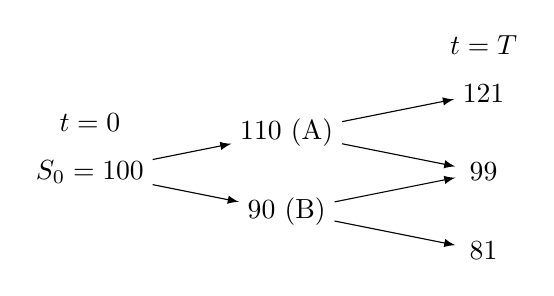
\begin{tikzpicture}[
                   grow = right,
edge from parent/.style = {draw,-latex},
         label distance = 1.5mm,
      every node/.style = {minimum width=2em, inner sep=3pt},
         level distance = 25mm,
       sibling distance = 10mm,
                     ]
\node[label=90:{$t=0$}] {$S_0=100$}
    child {node {90 (B)}
        child {node {81}
            %child {node {40}}
            %child {node {20}}
                }
        child {node {}}%<---------------- already printed
            }
    child {node[label=90:{}] {110 (A)}
        child {node {99}
            %child {node {}}%<------------ already printed
            %child {node {0}}
                }
        child {node[label=90:{$t=T$}] {121}
            %child {node {}}%<------------ already printed
            %child {node[label=90:{$t=3$}] {0}}
                }
                };
    \end{tikzpicture}
    \end{center}
    Assume that $R=1\%$ per year and that $T=2$ years. The payoff of the corresponding European put option is $(K-S)^+=(0,1,19)$. The tree is stationary, so the risk neutral probability weight is given by
    \begin{equation*}
        q = \dfrac{e^{RT}-d}{u-d} = \dfrac{e^{0.01\cdot1}-0.9}{1.1-0.9}
    \end{equation*}
    The price in node (A) is given by
    \begin{align*}
        P^{AM}_{(A)} &= \max\bigg\{(100-110)^+,e^{-0.01}\mathbb{E}^{\Qmeas}\left[\binom{0}{1}\right] \bigg\} \\
        &= \max\{0,e^{-0.01}(0\cdot q +1\cdot(1-q))\} \\
        &= e^{-0.01}(1-q)
    \end{align*}
    So it is better to wait when we arrive in node (A). If we are in node (B) we have:
    \begin{align*}
        P^{AM}_{(B)} &= \max\{(100-90)^+, e^{-0.01}(0\cdot q +1\cdot(1-q))\} \\ 
        &= 10
    \end{align*}
    So in node (B) it is better to exercise the option. Finally, the initial value of the American put option is:
    \begin{align*}
        P^{AM}_{0} &= \max\{(100-100)^+, e^{-0.01}(P^{AM}_{(A)}\cdot q +P^{AM}_{(B)}\cdot(1-q))\} \\ 
        &= e^{-0.01}[e^{-0.01}q(1-q)+10(1-q)] = \colorbox{cyan}{conti}
    \end{align*}
    If we compute the initial price of the European option we will find that
    $P^{AM}_{0}>P^{EU}_{0}$. This makes sense because for the American option it was convenient to exercise before the maturity (at least for one state of the nature), so we can really exploit this possibility.\\
    In terms of hedging, we only have to understand which are $\Delta_{0,(A)}$ and $\beta_{0,(A)}$. Since in node (B) the underlying decreases, there is no need to consider hedging in node (B).
\end{example}

%%%%%%%%%%%%%%%%%%%%% END OF DISCRETE TIME PART %%%%%%%%%%%%%%%%%%%%% 
\chapter{Continuous time finance}\lesson{9}{27/03/2020}
\section{Stochastic integrals}% pag. 300 in poi Hull
The starting point for finance in continuous time is a probability space $$(\Omega,\mathcal{F},\{\mathcal{F}_t\}_{t\ge0},\mathbb{P}),$$ where $\{\mathcal{F}_t\}_{t\ge0}$ is an increasing family of complete $\sigma$-algebras. Here, in order to avoid measurability problems, we assume also that $\{\mathcal{F}_t\}_{t\ge0}$ has right continuity:
\begin{equation*}
    \bigcap_{\epsilon>0}\mathcal{F}_{t+\epsilon}=\mathcal{F}_{t^+} = \mathcal{F}_t
\end{equation*}
This means that the information available immediately after $t$ coincides with the one at time $t$, so there can be shocks only in the left side of the limit, which can be discontinuous. This is a quite heavy assumption, because it involves the future, but it is compulsory. In this probability space we define the underlying stochastic process $X_t$ and we assume measurability with respect to the probability infrastructure and regularity in terms of the trajectory. In particular, we assume that $X_t$ is a \emph{RCLL} function, also called \emph{càdlàg}, i.e. a function defined on the real numbers (or a subset of them) that is right-continuous everywhere and has left limits everywhere.
\begin{figure}[htp]
    \centering
    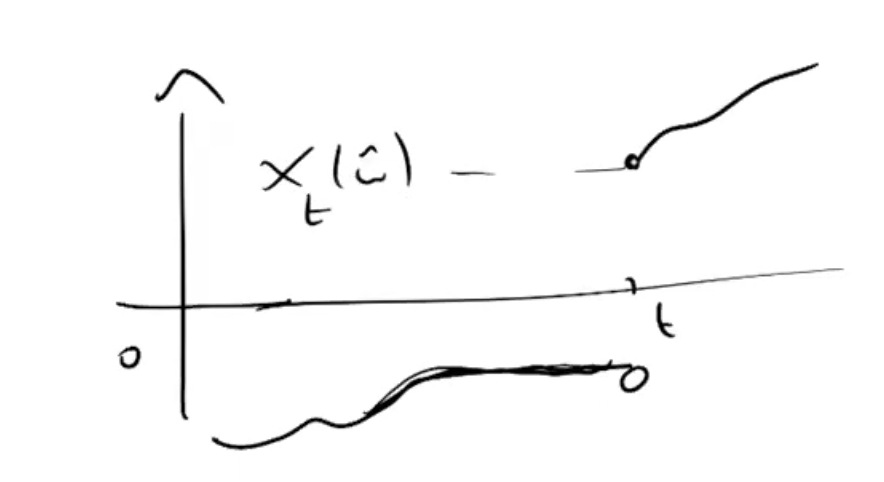
\includegraphics[scale=0.3]{fig/tmp/fig9.png}
    \caption{Càdlàg.}
    \label{fig:càdlàg}
\end{figure}
\newline Processes like this define a \emph{Brownian motion} $W_t$, i.e. a gaussian process with distribution at fixed time $\hat{t}$ $W_{\hat{t}}\sim\mathcal{N}(0,\hat{t})\sim\sqrt{\hat{t}}\mathcal{N}(0,1)$. Then we can define the stochastic integral
\begin{equation*}
    \int_0^t H_s\,``\dd W_s"
\end{equation*}
where $H\in\mathcal{H}$, being $\mathcal{H}$ the class of adapted processes such that $\mathbb{E}[\int_0^t H^2_s\,\dd s]<\infty$.
% completare questa parte mettendo qualcosa degli appunti di models, anche riguardo al fatto che il Brownian motion non è differenziabile ma si può definire una misura e calcolare formalmente un integrale bla bla bla
Since the Brownian motion is not differentiable it is not possible to define a differential. However, if we are able to define the integral with respect to the Brownian motion then we can define the differential operator as the derivative of the integral:
\begin{equation*}
    \dd\left(\int^t_0 H_s \dd W_s\right) \to H_t``\dd W_t"
\end{equation*}
\begin{example}{}{}{}
    Consider a process given by the deterministic integral
    \begin{equation*}
        X_t = \int^t_0 W_s\dd s
    \end{equation*}
    where $W_s$ is a Brownian motion. We want to show that $X_t$ behaves like a gaussian random variable $\mathcal{N}(\mu,\sigma)$ where $\mu, \sigma$ have to be determined. To solve the integral we can use \emph{Itô's Lemma}:
    \begin{equation*}
        \dd(tW_t) = W\dd t + t\,\dd W_t + \underbrace{\dd\langle\cdot,W_{\cdot}\rangle_t}_{\sim 0}
    \end{equation*}
    where $t$ is deterministic and the last term -- the quadratic covariance -- can be neglected because it leads to higher order terms in $\dd t$ (recall that $\dd t\dd W = \dd t\sqrt{\dd t}$). Integrating by parts we get:
    \begin{equation*}
        tW_t = \int^t_0 W_s\,\dd s + \int^t_0 s\,\dd W_s
    \end{equation*}
    So we can say that the integral
    \begin{equation*}
        \int^t_0 W_s\dd s = tW_t - \int^t_0 s\,\dd W_s
    \end{equation*}
    is Guassian, being the sum of two gaussian terms. \\
    Alternatively, recall that it is always possible to consider the Brownian motion as the integral of its differential, in fact we can define the integral operator to be compatible with the differential one:
    \begin{equation*}
        W_t = \int^t_0 \dd W_s = W_t - W_0
    \end{equation*}
    So, we can write:
    \begin{align*}
        \int^t_0 W_s\dd s &= \int^t_0\left(\int^s_0 \dd W_u\right)\,\dd s \overset{(a)}{=} \int^t_0\left(\int^t_u \dd s\right)\dd W_u \\
        &=
        \int^t_0(t-u)\,\dd W_u = tW_t - \int^t_0\dd W_u
    \end{align*}
    where in (a) we used the Stochastic Fubini Theorem to change the order of integration.\\
    Now we look for $\mu$ and $\sigma$. We have that
    \begin{equation*}
        \mathbb{E}[X_t] = \mathbb{E}\left[\int^t_0 W_s\,\dd s \right] \overset{(a)}{=} \int^t_0 \mathbb{E}[W_s]\dd s \overset{(b)}{=} 0
    \end{equation*}
    where in (a) we moved the expectation value inside the integral (we can do it because it is a deterministic integral) and in (b) we used the fact that by definition $\mathbb{E}[W_s] = 0$. Then:
    \begin{align*}
        \Var(X_t) &= \mathbb{E}\left[\left(\int^t_0 W_s\,\dd s \right)^2\right] = \mathbb{E}\left[\int^t_0\int^t_0 W_sW_u\,\dd s\,\dd u \right]\\
        &=
        \int^t_0\int^t_0 \mathbb{E}[W_sW_u]\dd s\,\dd u =
        \int^t_0\int^t_0 \Cov(W_s,W_u)\dd s\,\dd u
        \intertext{The increments of the Brownian motion are independent but the brownian motion itself is a strongly autocorrelated process, with covariance $\Cov(W_t,W_u)=\min\{s,u\}$. So we can write:}
        &=
        \int^t_0\left(\int^u_0 s\,\dd s+\int^t_u u\,\dd s\right)\dd u = \int^t_0\left(\dfrac{u^2}{2}+u(t-u)\right)\dd u \\
        &=
        \dfrac{t^3}{6}+\dfrac{t^3}{2}-\dfrac{t^3}{3} =  \dfrac{t^3}{3}
    \end{align*}
    So $X_t\sim\mathcal{N}(0,\nicefrac{t^3}{3})$.\\
    \textbf{Warning!} In this example we are able to do the computations -- in particular we can switch expected value and integration -- because we are dealing with deterministic integrals. If we have a stochastic integral, e.g. $\int^t_0H_s\dd W_s$, we cannot move the expected value inside the integral because we get something which is random:
    \begin{equation*}
        \underbrace{\mathbb{E}\left[\int^t_0H_s\dd W_s\right]}_{deterministic} \ne \underbrace{\int^t_0\mathbb{E}[H_s]\dd W_s}_{stochastic}.
    \end{equation*}
\end{example}
\noindent An important property is that if $H_s\in\mathcal{H}$, then the stochastic process $$\left(\int^t_0H_s\dd W_s\right)_{t\ge0}$$
is a martingale:
\begin{equation}
    \mathbb{E}\left[\int^t_0H_s\dd W_s\right] = \int^0_0H_s\dd W_s = 0.
\end{equation}
Luckily, $\mathcal{H}$ is a very rich class which contains also Brownian motions. In fact:
\begin{align*}
    \mathbb{E}\left[\int^t_0W_s^2\dd s\right] &= \int^t_0\mathbb{E}[W_s^2]\,\dd s = \int^t_0\Var(W_s)\,\dd s = \int^t_0s\,\dd s = \dfrac{t^2}{2} < \infty.
\end{align*}
We can extend the notion of stochastic integral even when $H_s\notin\mathcal{H}$, requiring a weaker condition, i.e.
\begin{equation*}
    H_s \in \Tilde{\mathcal{H}} = \bigg\{H\mbox{ adapted }: \mathbb{P}\left(\int_0^t H^2_s\,\dd s <\infty\right)=1\bigg\},
\end{equation*}
but in this case $X_t$ is a \emph{local martingale}, meaning that it is a martingale only for a specific set of stopping times. This means, in principle, that $\mathbb{E}[X_t]\ne0$.\\
Now, consider a Geometric Brownian Motion (GBM)
\begin{equation}
    \begin{cases}
    \dd X_t = \alpha X_t\, \dd t + \sigma X_t\, \dd W_t\\
    X_0 = x_0,
    \end{cases}
\end{equation}
which also can be written as
\begin{equation}
    X_t - x_0 = \alpha\int^t_0 X_s\, \dd s + \sigma\int^t_0 X_s \,\dd W_s.
\end{equation}
Since we are dealing with stochastic integrals, trivial integration is not possible and we have to find an other way to compute them. \\
First, let's consider the case in which $\sigma=0$. We get a linear deterministic equation:
\begin{equation}
    \dd X_t = \alpha X_t\, \dd t
\end{equation}
which can be written as
\begin{equation}
    \Dot{X}_t = \dv{X_t}{t} = \alpha X_t
\end{equation}
and has solution
\begin{equation}\label{detsol}
    X_t = x_0e^{\alpha t}.
\end{equation}
If $\sigma\ne0$ it is as we introduce a white noise which disturbs the evolution of the deterministic solution. The naive approach is to write the solution as
\begin{equation}
    X_t = ``x_0e^{\alpha t + \sigma W_t}"
\end{equation}
This is not correct, becayse it means that we are considering the exponential in a deterministic way, which is not the case. We have to use Itô's Formula.
\begin{theorem}[Itô's Formula]
    Assume that the process $X$ has a stochastic differential given by
    \begin{equation}
    \begin{cases}
        \dd X_t = K_t\, \dd t + H_t\, \dd W_t\\
        X_0 = x_0
    \end{cases}
    \end{equation}
    where $\alpha$ and $\sigma$ are adapted processes ($\alpha,\sigma\in\Tilde{\mathcal{H}}$), and let $f$ be a $C^{1,2}$ function. Define the process $Z(t) = f(t,X(t))$. Then $Z$ has a stochastic differential given by
    \begin{equation}\label{ito}
        \dd f=\left({\frac{\partial f}{\partial t}}+K_{t}{\frac {\partial f}{\partial x}}+{\frac{H_{t}^{2}}{2}}{\frac{\partial ^{2}f}{\partial x^{2}}}\right)\dd t+H_{t}{\frac{\partial f}{\partial x}}\,\dd W_{t}.
    \end{equation}
\end{theorem}
In our case, we take $f$ as the function which simplifies the deterministic part, which is an exponential. So, we take:
\begin{equation}
    f(t,X_t) = \ln X_t.
\end{equation}
According to \eqref{ito}, the differential is:
\begin{align}
    \notag \dd\ln{X_t} &= \dfrac{1}{X_t}\,\dd X_t + \dfrac{1}{2}\left(-\dfrac{1}{X_t^2}\right)\,\dd \expval{X_t}_t \\
    &=
    \notag \alpha\,\dd t + \sigma\,\dd W_t - \dfrac{1}{2X_t^2}(\sigma^2X_t^2\,\dd t)\\
    &=
    \left(\alpha-\dfrac{1}{2}\sigma^2\right)\,\dd t + \sigma\,\dd W_t
\end{align}
and integrating both sides we get:
\begin{equation}
    \ln X_t - \ln X_0 = \left(\alpha-\dfrac{1}{2}\sigma^2\right)t + \sigma(W_t-W_0) = \left(\alpha-\dfrac{1}{2}\sigma^2\right)t + \sigma W_t
\end{equation}
By taking the exponential of both sides we get:
\begin{equation}\label{stocsol}
    X_t = x_0e^{\left(\alpha-\frac{1}{2}\sigma^2\right)t + \sigma W_t}
\end{equation}
Notice that this solution is log-normal:
\begin{equation*}
    X_t \sim e^{\mathcal{N}\left(\ln x_0 + \left(\alpha-\frac{1}{2}\sigma^2\right)t, \sigma^2 t\right)}
\end{equation*}
and that it fluctuates around the corresponding deterministic solution \eqref{detsol}. We can demonstrate that averaging \eqref{stocsol} we get exactly \eqref{detsol}, in fact -- according to the moment generating function formula ${M(t)=\mathbb{E}[e^{tX}]=e^{\mu t}e^{{\frac {1}{2}}\sigma^{2}t^{2}}}$ -- the expected value of $e^{-\frac{1}{2}\sigma^2 t + \sigma W_t}$ is:
\begin{equation*}
    \mathbb{E}\left[e^{-\frac{1}{2}\sigma^2 t + \sigma W_t}\right] = \mathbb{E}\left[
    e^{\mathcal{N}\left(-\frac{1}{2}\sigma^2 t, \sigma^2 t\right)}\right] = e^{-\frac{1}{2}\sigma^2 t + \frac{1}{2}\sigma^2 t} = 1
\end{equation*}
Alternatively, one may recognize that $e^{-\frac{1}{2}\sigma^2 t + \sigma W_t}$ is a famous exponential martingale $Y_t$, and so $\mathbb{E}[Y_t]=Y_0=e^0 = 1$.

\subsection{Black \& Scholes market} % pag. 321 Hull
In the early 1970s, Fischer Black, Myron Scholes and Robert Merton achieved a major breakthrough in the pricing of European stock options. This was the development of what has become known as the Black–Scholes–Merton (Black \& Scholes) model.
This model describes the asset price $S_t$ in terms of the infinitesimal return $\frac{\dd S_t}{S_t}$, assuming that percentage changes in the stock price in a very short period of time are normally distributed. If we define a drift $\mu$ as the \emph{expected return of a stock per year}  and $\sigma$ as the \emph{volatility of the stock price per year} (a measure of our uncertainty about the returns provided by the stock), we have that
\begin{equation}\label{bs}
    \frac{\dd S_t}{S_t} = \mu \dd t + \sigma\dd W_t
\end{equation}
where $\dd W_t$ represents the noise given by this variability. The mean and standard deviation of the return in time $\dd t$ are approximately $\mu\dd t$ and $\sigma\sqrt{\dd t}$, so that
\begin{equation}
    \frac{\dd S_t}{S_t} \sim \mathcal{N}(\mu\dd t, \sigma^2\dd t)
\end{equation}
Recalling what we saw in the previous section, this implies that the return $Y_t = \ln S_t$ is normally distributed:
\begin{equation}
    \ln S_t \sim\mathcal{N}\left(\ln S_0+\left(\mu-\dfrac{\sigma^2}{2}\right)t,\sigma^2 t\right)
\end{equation}
and so $S_t$ is log-normal distributed.
\begin{figure}[htp]
    \centering
    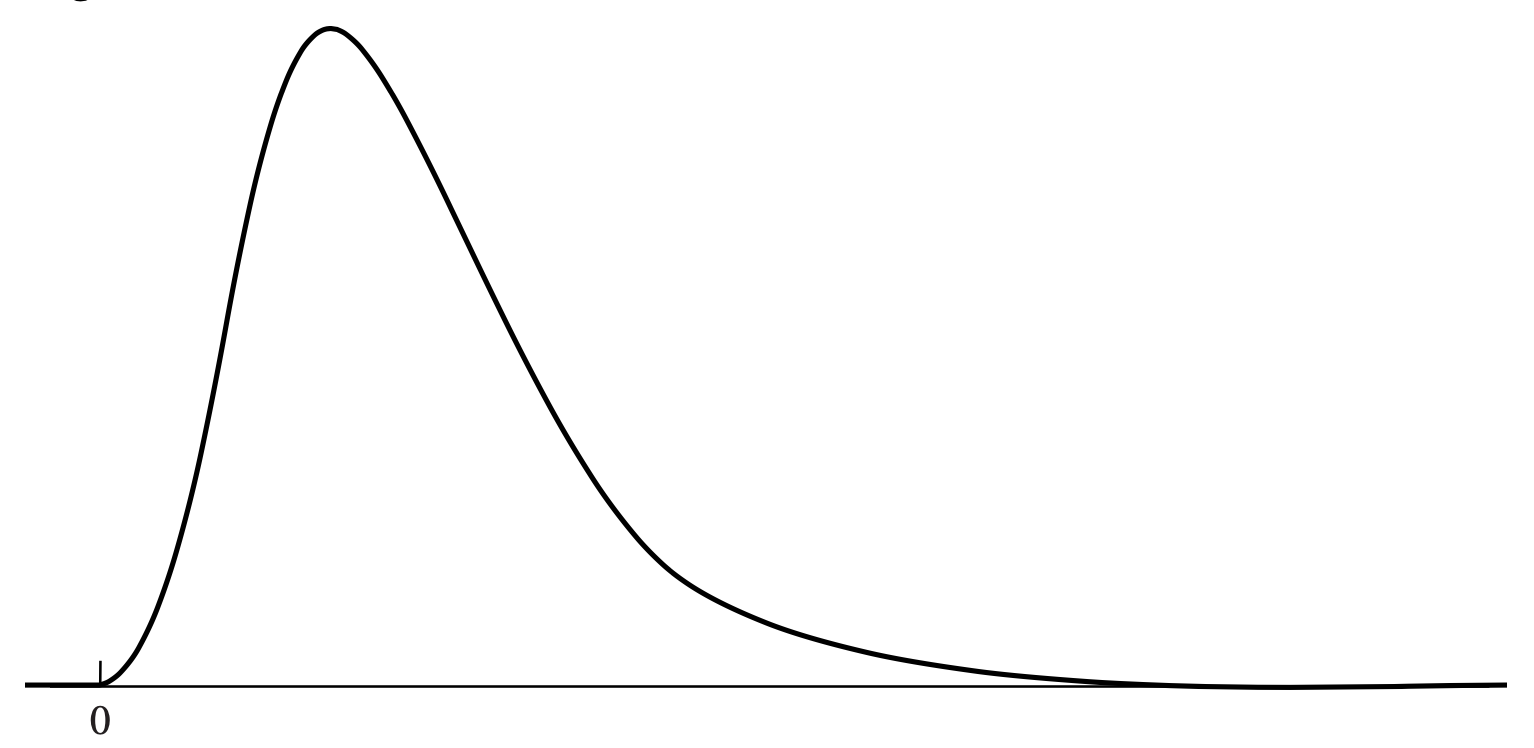
\includegraphics[scale=0.2]{fig/log_norm_distr.png}
    \caption{Log-normal distribution}
    \label{fig:lognorm}
\end{figure}
\newline While it is possible to estimate the historical volatility of the market, it is not possible to estimate the historical drift because it is not observable and also not stable. In fact, according to the particular time window we are considering, $\mu$ can assume different values.
\begin{figure}[htp]
    \centering
    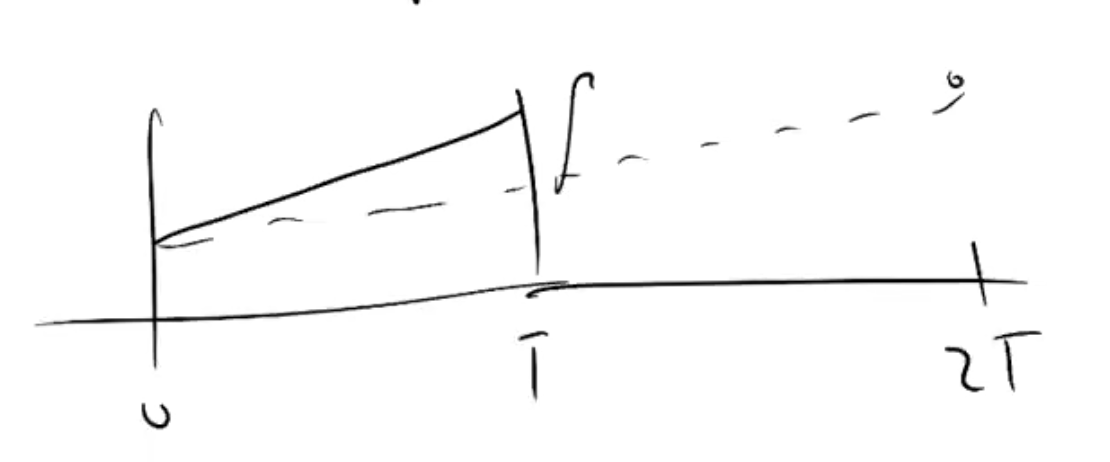
\includegraphics[scale=0.3]{fig/tmp/fig11.png}
    \caption{Different values of $\mu$.}
    \label{fig:mu}
\end{figure}
\newline In conclusion, we cannot jointly estimate $\mu$ and $\sigma$ from only one time series and we would like to get results which are independent of the drift (which plays the same role as the subjective probability in the static binomial model).

\subsection{The Girsanov Theorem} % pag. 162 Bjork
We want to find a way to switch from the subjective probability measure $\mathbb{P}$ to $\mathbb{Q}$ in continuous time. The tool that allows us to do that is the Girsanov Theorem.\\
Consider a Brownian motion $W_t^{\mathbb{P}}$ under the probability measure $(\Omega, \mathcal{F}, \mathbb{P})$ and a \emph{finite variation process} $\int^t_0 H_s\,\dd s$ (its differential has not a diffusion part). Then
\begin{equation}
    W_t^{\mathbb{Q}} \coloneqq W_t^{\mathbb{P}} - \int^t_0 H_s\,\dd s
\end{equation}
is not a Brownian motion under the measure $\mathbb{P}$, because it is not a martingale. However, it is a Brownian motion under the measure $\mathbb{Q}$, where
\begin{equation}\label{RN}
    \eval{\dv{\mathbb{Q}}{\mathbb{P}}}_t = \exp\left(\int^t_0 H_s\,\dd W_s^{\mathbb{P}}-\dfrac{1}{2}\int^t_0 H_s^2\,\dd s\right) \coloneqq Z_t
\end{equation}
is a process that satisfies the stochastic differential equation (SDE)
\begin{equation}
    \dd Z_t = H_t Z_t\,\dd W_t^\mathbb{P}
\end{equation}
and can be written as a constant plus a stochastic integral, which at least is a local martingale:
\begin{equation}
    Z_t = Z_0 + \int_0^t H_s Z_s\,\dd W_s^{\mathbb{P}}
\end{equation}
Eq. \eqref{RN} is called \emph{Radon-Nikodym derivative}: the choice of notation and the name of the function reflects the fact that it is analogous to a derivative in calculus, in the sense that it describes the rate of change of density of one measure with respect to another\footnote{See \url{https://en.wikipedia.org/wiki/Radon\%E2\%80\%93Nikodym_theorem}}. \\
One possible issue is that in the change from $\mathbb{P}$ to $\mathbb{Q}$ there can be a loss of probability mass, ending up with a $\mathbb{Q}$ which is not normalized to 1. In order to avoid that, $\int_0^t H_s Z_s\,\dd W_s^{\mathbb{P}}$ must be a global martingale. This is the assumption of Girsanov Theorem.
\begin{theorem}[Girsanov Theorem]
    Consider a Brownian motion under a probability measure $\mathbb{P}$. Then, a candidate Brownian motion under a different probability measure $\mathbb{Q}$ is a true $\mathbb{Q}$-Brownian motion if the change of measure characterized by $Z_t$ is a true martingale.
\end{theorem}
One consequence of this theorem is that changing measure is equivalent to shift the Brownian motion by a finite variation process. If we want to move from a probability measure to another, the effect on the SDE involves the drift, not the volatility.\\
How can we check the true martingality condition on $Z_t$? We know that if $H_sZ_s\in\mathcal{H}$ then $\int H_sZ_s\,\dd W_s$ is a martingale, but we cannot use this information because it involves $Z_s$ itself, which is unknown. In order to do that we use the \emph{Novikov condition}.
\begin{lemma}[Novikov condition]
    If
    \begin{equation}
        \mathbb{E}\left[e^{\frac{1}{2}\int^t_0 H_s^2\,\dd s}\right]<\infty
    \end{equation}
    then $Z_t$ is a true martingale.
\end{lemma}
\textbf{Summary.} In conclusion, suppose that $X$ is a random variable and we want to compute
\begin{equation*}
    \mathbb{E}[X] = \int_{\Omega}X\,\dd\mathbb{P} = \int_{\Omega}X(\omega)\mathbb{P}(\dd\omega).
\end{equation*}
If we don't know the distribution of $X$ under the probability measure $\mathbb{P}$ but we know it under an other probability measure $\mathbb{Q}$, it is possible to switch from $\mathbb{P}$ to $\mathbb{Q}$ using the change of measure
\begin{equation*}
    \mathbb{E}^{\mathbb{P}}[X] = \int X\dv{\mathbb{P}}{\mathbb{Q}}\,\dd\mathbb{Q} = \mathbb{E}^{\mathbb{Q}}\left[X\dv{\mathbb{P}}{\mathbb{Q}}\right]
\end{equation*}
This holds for all $X$. In particular, if we take $X=1$ then
\begin{equation*}
    1 = \mathbb{E}^{\mathbb{P}}[1] = \mathbb{E}^{\mathbb{Q}}\left[\dv{\mathbb{P}}{\mathbb{Q}}\right]
\end{equation*}
So, in order to avoid loss of probability mass, $\dv{\mathbb{P}}{\mathbb{Q}}$ must be a true martingale.

\section{Portfolio dynamics}\lesson{10}{01/04/2020} % ch. 6 Bjork
Let us consider a financial market consisting of different assets such as stocks, bonds with different maturities, or various kinds of financial derivatives. In this section we will take the price dynamics of the various assets as given, and the main objetive is that of deriving the dynamics of (the value of) a so-called \emph{self financing portfolio}. In continuous time this turns out to be a fairly delicate task, so we start by studying a model in discrete time. We will then let the length of the time step tend to zero, thus obtaining the continuous time analogs. \\
Let us thus study a financial market, where time is divided into periods of length $\Delta t$, and where trading only takes place at the discrete points in time $n\Delta t$, $n = 0, 1,\dots$. We consider a fixed period $[t, t + \Delta t)$. This period is henceforth referred to as “period $t$”. 
\begin{definition} Let's define the following notation:
    \begin{itemize}
    \item $N =$ the number of different types of stocks.
    \item $h_i(t) =$ number of shares of type $i$ held during the period $[t, t + \Delta t)$.
    \item $h(t) =$ the portfolio $[h_1(t),\dots,h_N(t)]$ held during period $t$.
    \item $c(t) =$ the amount of money spent on consumption per unit time during the period $[t, t + \Delta t)$.
    \item $S_i(t) =$ the price of one share of type $i$ during the period $[t, t + \Delta t)$.
    \item $V(t) =$ the value of the portfolio $h$ at time $t$.
    \end{itemize}
\end{definition}
The information and the decisions in the model are structured as follows:
\begin{itemize}
    \item At time $t$, i.e. at the start of period $t$, we bring with us an “old” portfolio $h(t - \Delta t) = \{h_i(t - \Delta t), i = 1,\dots,N\}$ from the previous period $t - \Delta t$.
    \item At time $t$ we can observe the price vector $S(t)=(S_1(t),\dots,S_N(t))$.
    \item At time $t$, after having observed $S(t)$, we choose a new portfolio $h(t)$, to be held during period $t$. At the same time we also choose the consumption rate $c(t)$ for the period $t$. Both $h(t)$ and $c(t)$ are assumed to be constant over the period $t$.
\end{itemize}
\begin{remark}
    We only consider non-dividend paying assets.
\end{remark}
To start the analysis we observe that the wealth at the
start of period $t$, $V(t)$, equals the value of the old portfolio $h(t - \Delta t)$. Thus we have:
\begin{equation}\label{6.1}
    V(t) = \sum^N_{i=1}h_i(t-\Delta t)S_i(t) = h(t-\Delta t)S(t)
\end{equation}
This equation simply says that at the beginning of period $t$ our wealth equals what we get if we sell our old portfolio at today's
prices. We may now use the proceeds of this sale for two purposes:
\begin{enumerate}
    \item Reinvest in a new portfolio $h(t)$.
    \item Consume at the rate $c(t)$ over the period $t$
\end{enumerate}
The cost of the new portfolio $h(t)$, which has to be bought at today’s prices, is given by
\begin{equation}
    \sum^N_{i=1} h_i(t)S_i(t) = h(t)S(t)
\end{equation}
whereas the cost for the consumption rate $c(t)$ is given by $c(t)\Delta t$. The \emph{budget equation} for period $t$ thus reads
\begin{equation}
    h(t-\Delta t)S(t) = h(t)S(t) + c(t)\Delta t
\end{equation}
\begin{equation*}
    (h(t)-h(t-\Delta t)S(t) + c(t)\Delta t = 0
\end{equation*}
\begin{equation}\label{6.3}
    \Delta h(t)S(t) + c(t)\Delta t = 0
\end{equation}
Since our goal is to obtain the budget equation in continuous time it is now tempting to let $\Delta t \to 0$ in eq. \eqref{6.3} to obtain the formal expression
\begin{equation}
    S(t)\dd h(t) + c(t)\dd t = 0.
\end{equation}
This procedure is, however, \textbf{not correct}. In fact, all the stochastic differentials are to be interpreted in the Itô sense and the Itô integral $\int H(t)\dd W(t)$ was defined as the limit of sums of the type $\sum H(t_n)[W(t_{n+1})-W(t_n)]$ where it was essential that the $W$-increments were forward differences. But in eq. \eqref{6.3} we have a backward $h$-difference.\\
In order to get Itô differentials we thus have to reformulate eq. \eqref{6.3}. This is done by adding and subtracting the term $S(t- \Delta t)\Delta h(t)$ to the left-hand side:
\begin{align*}
    \Delta h(t)S(t) + c(t)\Delta t + S(t- \Delta t)\Delta h(t) - S(t- \Delta t)\Delta h(t) = 0
\end{align*}
\begin{equation*}\label{6.4}
    S(t - \Delta t)\Delta h(t)+\Delta S(t)\Delta h(t) + c(t)\Delta t = 0
\end{equation*}
Now, at last, we may let $\Delta t \to 0$ in the budget eq. \eqref{6.4}, giving us
\begin{equation}\label{6.7}
    S(t)\dd h(t) + \dd h(t)\dd S(t) + c(t)\dd t = 0.
\end{equation}
Letting $\Delta t \to 0$ in eq. \eqref{6.1} gives us 
\begin{equation}
    V(t) = h(t)S(t)
\end{equation}
and if we take the Itô differential of this expression we get
\begin{align}
    \notag \dd V(t) &= h(t)\dd S(t) + S(t)\dd h(t) + \dd S(t)\dd h(t) \\
    \overset{\eqref{6.7}}&{=}
    \notag h(t)\dd S(t) + S(t)\dd h(t) - c(t)\dd t - S(t)\dd h(t) \\
    &=
    S(t)\dd h(t) - c(t)\dd t
\end{align}
In particular, in a situation without any consumption we have the following V-dynamics:
\begin{equation}\label{6.9}
    \dd V(t) = h(t)\dd S(t).
\end{equation}
This is the so called \emph{self-financing portfolio}, i.e. a portfolio with no exogenous infusion or withdrawal of money. In other words, the purchase of a new portfolio, as well as all consumption, must be financed solely by selling assets already in the portfolio.\\
The natural economic interpretation of eq. \eqref{6.9}) is that in a model without any exogenous income, all change of wealth is due to changes in asset prices. In other words, the fact that the portfolio fluctuates does not depend on our strategy $h$ but only on the fact that in a infinitesimal interval there has been a fluctuation in the market due to a shock in the risky asset.

\section{Option pricing in the Black \& Scholes model} % ch. 7 Bjork
Let us consider a financial market consisting of only two assets: 
\begin{enumerate}
    \item A savings account (risk free asset) with price process $B$
    that evolves according to the deterministic equation
    \begin{equation}
        \dfrac{\dd B_t}{B_t} = r \dd t;
    \end{equation}
    \item A stock with price process (risky asset) $S$, evolving according to the Brownian motion SDE
    \begin{equation}\label{bmsde}
        \dfrac{\dd S_t}{S_t} = \mu \dd t + \sigma \dd W_t
    \end{equation}
    where $\sigma\ne0$, otherwise if $\mu\ne r$ there is an arbitrage opportunity.
\end{enumerate}
In the Black \& Scholes model $\mu,\sigma$ and $r$ are constant. We make the following assumptions:
\begin{itemize}
    \item The derivative can be bought or sold without any restriction;
    \item There is no arbitrage opportunity;
    \item The price can be written as a function of the underlying:
    \begin{equation}
        price_t = p(t) = F(t,S(t))\in C^{1,2}.
    \end{equation}
    This is a Markovian-like assumption, which is quite strong because it says that the price depends only on the current value of the underlying $S(t)$, which is not true in general. 
\end{itemize}
The idea is to repeat the same argument we used in the discrete time framework. So we want to construct the replicating portfolio of the payoff at time $T$ and it must be self-financing, otherwise the initial value of the option may be different from the value of our portfolio if in the meanwhile we receive something else. We write the value of the replicating portfolio at time $t$ as 
\begin{equation}\label{v}
    V(t) = \alpha(t)S(t) + \beta(t)B(t) = F(t,S(t))
\end{equation}
At maturity we have
\begin{equation}
    V(T) = \mbox{payoff}_T
\end{equation}
Then, by absence of arbitrage opportunity it must be that
\begin{equation}
    V(0) = price_0(\mbox{payoff}_T) = p(0) = F(0,S(0))
\end{equation}
and this must hold also for all the intermediate times
\begin{equation}
    V(t) = F(0,S(0))
\end{equation}
So our constructed portfolio and the option have the same value at any time. This means that also the fluctuations, i.e. their differentials, are the same:
\begin{align}
    \dd V(t) = \dd F(t,S(t))
\end{align}
According to \eqref{6.9} we have that 
\begin{align}
    \notag \dd V(t) &= h(t)\dd S(t) = (\alpha, \beta)\binom{\dd S}{\dd B} \\ &=
    \notag \alpha\dd S+\beta\dd B\\
    &=
    \alpha(\mu S\dd t+\hlc{mypink}{\sigma\dd W})+\beta rB\dd t
\end{align}
and $\dd F(t,S(t))$ is given by the Itô's Formula:
\begin{align}
    \notag \dd F &= \pdv{F}{t}\dd t + \pdv{F}{S}\dd S + \dfrac{1}{2}\pdv[2]{F}{S}\dd\expval{S} \\
    \overset{\eqref{bmsde}}&{=} 
    \left(\pdv{F}{t} + \pdv{F}{S}\mu S + \dfrac{1}{2}\pdv[2]{F}{S}\sigma^2S^2\right)\dd t + \hlc{mypink}{\pdv{F}{S}\sigma S\dd W}
\end{align}
Comparing the two terms in pink we find that
\begin{equation}
    \alpha(t) = \pdv{F}{S} = \Delta(t)
\end{equation} 
so $\alpha$ is the equivalent of the difference in the value the option divided by the difference of the underlying ($\Delta$) in the discrete time framework.\\
Comparing the remaining terms we get:
\begin{equation}\label{342}
    \alpha(t)\mu S + \beta rB = \pdv{F}{t} + \pdv{F}{S}\mu S + \dfrac{1}{2}\pdv[2]{F}{S}\sigma^2S^2
\end{equation}
Multiply both sides of eq. \eqref{v} for $r$:
\begin{equation*}
    rV = r\alpha S + r\beta B
\end{equation*}
and then substitute in eq. \eqref{342}, recalling that $\alpha(t) = \pdv{F}{S}$ and $V(t)=F(t,S(t))\,\,\forall t$:
\begin{equation*}
    \cancel{\pdv{F}{S}\mu S} + rF - r\pdv{F}{S} S = \pdv{F}{t} + \cancel{\pdv{F}{S}\mu S} + \dfrac{1}{2}\pdv[2]{F}{S}\sigma^2S^2
\end{equation*}
We obtained the so called \emph{Black \& Scholes partial differential equation}:
\begin{equation}\label{BSpde}
    \begin{cases}
    \pdv{F(t,S(t))}{t} + r\pdv{F(t,S(t))}{S(t)} S(t) + \dfrac{1}{2}\pdv[2]{F(t,S(t))}{S(t)}\sigma^2S(t)^2 - rF(t,S(t))\\
    F(T,S(T)) = \mbox{payoff}_T
    \end{cases}
\end{equation}
We started with a generic derivative and we assumed that the price was a function $F(t,S(t))$ of the time and the current value of the underlying. Now we have found that -- in order to satisfy the absence of arbitrage opportunity -- $F$ obeys to the Black \& Scholes PDE. The only thing that characterizes a specific payoff is the terminal condition
\begin{equation}
    F(T,S(T)) = \mbox{payoff}_T
\end{equation}
So, for example, if we want to price a call option we have to solve the PDE \eqref{BSpde} with the terminal condition $F(T,S(T))=(S(T)-K)^+$.
\begin{remark}
    Notice that eq. \eqref{BSpde} is a deterministic equation. Of course, the solution fluctuates according to the Brownian motion but at any fixed time it is deterministic.
\end{remark}
By a change of variable, there is the possibility to reduce \eqref{BSpde} to the heat equation. However, we will use a different approach, which involves the \emph{Feynman-Kac formula}.
\begin{theorem}[Feynman-Kac formula, v1]
    Assume that $F\in C^{1,2}$ is a solution to the boundary value problem
    \begin{equation}\label{bvp}
        \begin{cases}
        \pdv{F(t,x)}{t} + \mu\pdv{F(t,x)}{x} + \dfrac{1}{2}\sigma^2\pdv[2]{F(t,x)}{x}=0\\
        F(T,x) = \Phi(x)
        \end{cases}
    \end{equation}
    where $x\in\mathbb{R}$ and $t\in[0,T]$. Then, provided that $\sigma\pdv{F(t,x)}{x}\in\mathcal{H}$, there exists a probability space $(\Omega,\mathcal{F},\mathbb{P})$ on which we can define a Brownian motion $(W_t)_{t\ge0}$ such that
    \begin{equation}
        F(t,x) = \mathbb{E}_{x,t}[\Phi(X_T)]
    \end{equation}
    where $X$ satisfies the SDE
    \begin{equation}\label{fk}
        \begin{cases}
        \dd X_s = \mu(s, X_s)\dd s + \sigma(s, X_s)\dd W_s\\
        X_t = x
        \end{cases}
    \end{equation}
\end{theorem}  
\begin{proof}
    We have that $F$ evolves according the Itô's Formula:
    \begin{align*}
        \dd F(t,x) &= \pdv{F}{t}\dd t + \pdv{F}{x}\dd x + \dfrac{1}{2}\pdv[2]{F}{x}\dd\expval{x}\\
        \overset{\eqref{fk}}&{=}
        \pdv{F}{t}\dd t + \pdv{F}{x}(\mu\dd t + \sigma \dd W) + \dfrac{1}{2}\pdv[2]{F}{x}\sigma^2 \dd t
    \end{align*}
    Taking the integral from $t$ to $T$ of both sides we get:
    \begin{align*}
        F(T,x) - F(t,x) &= \int^T_t \left(\pdv{F}{u} + \mu\pdv{F}{x} + \dfrac{1}{2}\pdv[2]{F}{x}\sigma^2 \right)\dd u + \int^T_t \pdv{F}{x}\sigma \dd W_u \\
        \overset{\eqref{bvp}}&{=}
        F(T,x) - F(t,x) = \int^T_t \pdv{F}{x}\sigma \dd W_u
    \end{align*}
    Now we want to remove the stochastic integral, so we take the expected value:
    \begin{equation*}
        \mathbb{E}_{t,x}[F(T,x)] - \mathbb{E}_{t,x}[F(t,x)] = \mathbb{E}_{t,x}\left[\int_t^T \pdv{F}{x}\sigma \dd W_u\right]
    \end{equation*}
    \begin{equation*}
        \mathbb{E}_{t,x}[F(T,x)] - F(t,x) = \mathbb{E}_{t,x}\left[\int_t^T \pdv{F}{x}\sigma \dd W_u\right]
    \end{equation*}
    We know that if $\pdv{F}{x}\sigma\in\mathcal{H}$ then the stochastic integral is a $\mathbb{P}$-martingale, so by the definition we have that
    \begin{equation*}
        \mathbb{E}_{t,x}\left[\int_t^T \pdv{F}{x}\sigma \dd W_u\right] = \int^t_t \pdv{F}{x}\sigma \dd W_u = 0
    \end{equation*}
    In the end, we get
    \begin{equation*}
        \mathbb{E}_{t,x}[F(T,x)] = F(t,x) \qquad\Rightarrow\qquad F(t,x) = \mathbb{E}_{x,t}[\Phi(X_T)].
    \end{equation*}
\end{proof}
We consider also another version which appears over and over again in the study of pricing problems for financial derivatives.
\begin{theorem}[Feynman-Kac formula, v2]
    Assume that F is a solution to the boundary value problem
    \begin{equation}\label{bvp1}
        \begin{cases}
        \pdv{F(t,x)}{t} + K\pdv{F(t,x)}{x} + \dfrac{1}{2}H^2\pdv[2]{F(t,x)}{x}-rF(t,x)=0\\
        F(T,x) = \Phi(x)
        \end{cases}
    \end{equation}
    where $x\in\mathbb{R}$, $t\in[0,T]$ and $r$ is a given real number. Then, provided that $$e^{-rt}H\pdv{F(t,x)}{x}\in\mathcal{H},$$ 
    there exists a probability space $(\Omega,\mathcal{F},\mathbb{P})$ on which we can define a Brownian motion $(W_t)_{t\ge0}$ such that
    \begin{equation}
        F(t,x) = e^{-r(T-t)}\mathbb{E}_{x,t}[\Phi(X_T)]
    \end{equation}
    where $X$ satisfies the SDE
    \begin{equation}\label{fk1}
        \begin{cases}
        \dd X_s = K(s, X_s)\dd s + H(s, X_s)\dd W_s\\
        X_t = x
        \end{cases}
    \end{equation}
\end{theorem}
\begin{proof}
    Let's consider the Itô development of the discounted value of $F$:
    \begin{align*}
        \dd(e^{-rt}F(t,x)) &= (-re^{-rt}\dd t)F + e^{-rt}F + \order{\dd t\dd W}\\
        &= 
        -re^{-rt}\dd tF + e^{-rt}F \\
        &=
        -re^{-rt}\dd tF + e^{-rt}\left(\pdv{F}{t}\dd t + \pdv{F}{x}\dd x + \dfrac{1}{2}\pdv[2]{F}{x}\dd\expval{x}\right) \\
        &=
        -re^{-rt}\dd tF + e^{-rt}\left(\pdv{F}{t}\dd t + \pdv{F}{x}K + \dfrac{1}{2}\pdv[2]{F}{x}H^2\right)\dd t + e^{-rt}\pdv{F}{x}H\dd W \\
        &=
        e^{-rt}\dd t\left(-rF + \pdv{F}{t}\dd t + \pdv{F}{x}K + \dfrac{1}{2}\pdv[2]{F}{x}H^2\right) + e^{-rt}\pdv{F}{x}H\dd W \\
        \overset{\eqref{bvp1}}&{=}
        e^{-rt}\pdv{F}{x}H\dd W
    \end{align*}
    Taking the integral from $t$ to $T$ of both sides we get:
    \begin{align*}
        e^{-rT}F(T,x) - e^{-rt}F(t,x) = \int^T_t e^{-rt}\pdv{F}{x}H \dd W_u
    \end{align*}
    Now we want to remove the stochastic integral, so we take the expected value:
    \begin{equation*}
        \mathbb{E}_{t,x}[e^{-rT}F(T,x)] - \mathbb{E}_{t,x}[e^{-rt}F(t,x)] = \mathbb{E}_{t,x}\left[\int_t^T e^{-rt}\pdv{F}{x}H \dd W_u\right]
    \end{equation*}
    \begin{equation*}
        \mathbb{E}_{t,x}[e^{-rT}F(T,x)] - e^{-rt}F(t,x) = \mathbb{E}_{t,x}\left[\int_t^T e^{-rt}\pdv{F}{x}H \dd W_u\right]
    \end{equation*}
    We know that if $e^{-rt}\pdv{F}{x}H\in\mathcal{H}$ then the stochastic integral is a $\mathbb{P}$-martingale, so by the definition we have that
    \begin{equation*}
        \mathbb{E}_{t,x}\left[\int_t^T e^{-rt}\pdv{F}{x}H \dd W_u\right] = 0
    \end{equation*}
    In the end, we get
    \begin{equation*}
        \mathbb{E}_{t,x}[e^{-rT}F(T,x)] = e^{-rt}F(t,x) \qquad\Rightarrow\qquad F(t,x) = e^{-r(T-t)}\mathbb{E}_{x,t}[\Phi(X_T)].
    \end{equation*}
\end{proof}

\begin{theorem}[Feynman-Kac formula, v3]\lesson{11}{02/04/2020} 
    Assume that $F$ is a solution to the boundary value problem
    \begin{equation}\label{bvp2}
        \begin{cases}
        \pdv{F(t,x)}{t} + K\pdv{F(t,x)}{x} + \dfrac{1}{2}H^2\pdv[2]{F(t,x)}{x}+g(t,x)=0\\
        F(T,x) = \Phi(x)
        \end{cases}
    \end{equation}
    Then, provided that $$H\pdv{F(t,x)}{x}\in\mathcal{H},$$ 
    there exists a probability space $(\Omega,\mathcal{F},\mathbb{P})$ on which we can define a Brownian motion $(W_t)_{t\ge0}$ such that
    \begin{equation}
        F(t,x) = \mathbb{E}_{x,t}[\Phi(X_T)] + \int^T_t \mathbb{E}_{x,t}[g(s,x_s)]\dd s
    \end{equation}
    where $X$ satisfies the SDE
    \begin{equation}\label{fk2}
        \begin{cases}
        \dd X_s = K(s, X_s)\dd s + H(s, X_s)\dd W_s\\
        X_t = x
        \end{cases}
    \end{equation}
\end{theorem}
\begin{proof}
    Apply Itô's Formula on $F$:
    \begin{align*}
        \dd F(t,x) &= \left(\pdv{F}{t} + \pdv{F}{x}K + \dfrac{1}{2}\pdv[2]{F}{x}H^2\right)\dd t + \pdv{F}{x}H\dd W\\
        \overset{\eqref{bvp2}}&{=}
        -g(t,x)\dd t + \pdv{F}{x}H\dd W
    \end{align*}
    Taking the integral from $t$ to $T$ of both sides we get:
    \begin{equation*}
        F(T,x) - F(t,x) = -\int^T_t g(s,x_s)\dd s + \int^T_t \pdv{F}{x}H \dd W_s 
    \end{equation*}
    Now we want to remove the stochastic integral, so we take the expected value:
    \begin{equation*}
        \mathbb{E}_{t,x}[F(T,x)] - F(t,x) = -\mathbb{E}_{t,x}\left[\int_t^T g(s,x_s)\dd s \right] + \mathbb{E}_{t,x}\left[\int_t^T \pdv{F}{x}H \dd W_s\right]
    \end{equation*}
    We know that if $H\pdv{F}{x}\sigma\in\mathcal{H}$ then the stochastic integral is a $\mathbb{P}$-martingale, so by the definition we have that
    \begin{equation*}
        \mathbb{E}_{t,x}\left[\int_t^T \pdv{F}{x}H \dd W_u\right] = 0
    \end{equation*}
    In the end, we get
    \begin{equation*}
        \mathbb{E}_{t,x}[F(T,x)] = F(t,x) - \left[\int_t^T \mathbb{E}_{t,x}[g(s,x_s)]\dd s \right] 
    \end{equation*}
    \begin{equation*}
        F(t,x) = \mathbb{E}_{x,t}[\Phi(X_T)] + \left[\int_t^T \mathbb{E}_{t,x}[g(s,x_s)]\dd s \right].
    \end{equation*}
\end{proof}
\begin{example}{}{}{}
    Solve the PDE 
    \begin{equation*}
        \begin{cases}
        \pdv{F}{t}(t,x) + \frac{\sigma^2}{2}\pdv[2]{F}{x}(t,x) = 0\\
        F(T,x) = x^2
        \end{cases}
    \end{equation*}
    where $\sigma$ is constant.\\
    \textbf{Solution.} In this case $K=0$ and $H=\sigma$, so the process $X$ follows the differential equation 
    \begin{equation}\label{331}
        \begin{cases}
        \dd X = \sigma\dd W_t. \tag{$\ast$}\\
        X_t = x
        \end{cases}
    \end{equation}
    Integrating \eqref{331} we get:
    \begin{equation*}
        X_T - x = \sigma(W_T - W_t) \quad\Rightarrow\quad X_T = x + \sigma(W_T - W_t)
    \end{equation*}
    Using the first version of the Feynman-Kac formula we have the solution:
    \begin{align*}
        F(t,x) &= \mathbb{E}_{x,t}[X^2_T] \\
        &=
        \mathbb{E}_{x,t}[x^2 + \sigma^2(W_T - W_t)^2 + 2x\sigma(W_T-W_t)] \\
        &= 
        x^2 + \sigma^2(T-t) + 0 = x^2 + \sigma^2(T-t)
    \end{align*}
    where we used the fact that the Brownian increment $(W_T - W_t)$ is independent of the filtration and that $(W_T-W_t)\sim \mathcal{N}(0,T-t)$, so $\dd W^2 = \dd t$ and $(W_T-W_t)=0$. However, we can not say that it is the solution yet, because we first have to check if $F$ satisfies the PDE:
    \begin{equation*}
        \begin{cases}
        \pdv{F}{t}(t,x) + \frac{\sigma^2}{2}\pdv[2]{F}{x}(t,x) = -\sigma^2 + \frac{\sigma^2}{2}2 = 0\\
        F(T,x) = x^2 + \sigma^2(T-T) = x^2
        \end{cases}
    \end{equation*}
    and then we have to check the regularity condition $\pdv{F}{x}H = 2X_t\sigma\in\mathcal{H}$, i.e. it must be that $\mathbb{E}\left[\int^T_0 (2X_t\sigma)^2\,\dd t\right] < \infty$:
    \begin{align*}
        \mathbb{E}\left[\int^T_0 (2X_t\sigma)^2\,\dd t\right] &= \int^T_0 4\sigma^2\mathbb{E}[X_t^2]\,\dd t \\
        &= 
        \int^T_0 4\sigma^2\mathbb{E}[(X_0+\sigma W_t)^2]\,\dd t \\
        &=
        4\sigma^2 \int^T_0 \mathbb{E}[X_0^2+\sigma^2 W_t^2 + 2X_0\sigma W_t]\,\dd t \\
        &=
        4\sigma^2 \int^T_0 (x_0^2+\sigma^2 t + 0)\,\dd t \\
        &=
        4\sigma^2\left(x_0^2 t +\frac{\sigma^2 T^2}{2}\right) < \infty \quad \forall T>0.
    \end{align*}
\end{example}
\begin{example}{}{}{}
    Solve the PDE
    \begin{equation*}
        \begin{cases}
        \pdv{F}{t}(t,x) + \frac{x^2}{2}\pdv[2]{F}{x}(t,x) + x = 0\\
        F(T,x) = \ln x^2
        \end{cases}
    \end{equation*}
    \textbf{Solution.} In this case $K=0$, $H=x$ and $g(t,x)=x$, so the process $X$ follows the SDE
    \begin{equation*}
        \begin{cases}
        \dd X_t = X_t\dd W_t\\
        X_t = x
        \end{cases}
    \end{equation*}
    which can be integrated from $t$ to $T$, obtaining:
    \begin{equation}\label{lin}
        X_T = X_t e^{-\frac{1}{2}(T-t)+W_T-W_t} \tag{$\star$}
    \end{equation}
    Using the Feynman-Kac formula v3 we have the solution
    \begin{align*}
        F(t,x) &= \mathbb{E}_{t,x}[\ln x^2] + \int_t^T \mathbb{E}_{t,x}[X_s]\,\dd s \\
        \overset{(*)}&{=} 
        \mathbb{E}_{t,x}\left[2\ln x + 2\left(-\frac{1}{2}(T-t)+W_T-W_t\right)\right] +\\
        &\qquad\qquad\qquad\qquad + \int_t^T \mathbb{E}_{t,x}[X_t e^{-\frac{1}{2}(s-t)+W_s-W_t}]\,\dd s \\
        \overset{(a)}&{=}
        2\ln x - (T-t) + x\int^T_t \mathbb{E}_{t,x}\left[e^{-\frac{1}{2}(s-t)+W_s-W_t}\right] \,\dd s \\
        \overset{(c)}&{=} 
        2\ln x - (T-t) + x\int^T_t e^{-\frac{1}{2}(s-t)} \mathbb{E}\left[e^{\mathcal{N}(0,s-t)}\right] \,\dd s \\
        \overset{(b)}&{=} 
        2\ln x - (T-t) + x\int^T_t e^{-\frac{1}{2}(s-t)}e^{\frac{1}{2}(s-t)} \,\dd s \\
        &=
        2\ln x - (T-t) + x(T-t) \\
        &= 
        \ln x^2 + (T-t)(x-1)
    \end{align*}
    where in (a) we used the fact that the expected value of $W_T-W_t$ is zero and in (b) we used the fact that since $W_s-W_t$ is independent of $\mathcal{F}_t$ we can remove the conditional expected value. In (c) we used the moment generating function formula ${M(t)=\mathbb{E}[e^{tX}]=e^{\mu t}e^{{\frac {1}{2}}\sigma^{2}t^{2}}}$. We also could have used the fact the the exponential in $(*)$ is an exponential martingale.\\
    Now we have to check that $F$ satisfies the PDF:
    \begin{equation*}
        \begin{cases}
        \pdv{F}{t}(t,x) + \frac{x^2}{2}\pdv[2]{F}{x}(t,x) + x = -x+1+\frac{x^2}{2}\left(-\frac{2}{x^2}\right)+x = 0\\
        F(T,x) = \ln x^2 + (T-T)(x-1) = \ln x^2
        \end{cases}
    \end{equation*}
    Then we have to check that $\pdv{F}{x}H = \left(\frac{2}{X_t}+T-t\right)X_t\in\mathcal{H}$ \colorbox{cyan}{fai conti}:
    \begin{equation*}
        \mathbb{E}\left[\int^T_0 (2 + X_t(T-t))^2\,\dd t\right] \overset{\eqref{lin}}{=} \int^T_0 e^{-linear(t)}\,\dd t < \infty
    \end{equation*}
\end{example}
Let's consider the Black \& Scholes PDE
\begin{equation}
    \begin{cases}
    \pdv{F(t,S(t))}{t} + r\pdv{F(t,S(t))}{S(t)} S(t) + \dfrac{1}{2}\pdv[2]{F(t,S(t))}{S(t)}\sigma^2S(t)^2 - rF(t,S(t))\\
    F(T,S(T)) = \mbox{payoff}_T
    \end{cases}
\end{equation}
By the Feynman-Kac formula v2 we know that if a function is a solution of the previous equation then we can associate the problem of solving a PDE to the problem of computing an expected value:
\begin{equation}
    F(t,S(t)) = e^{-r(T-t)}\mathbb{E}^{\hat{\mathbb{P}}}_{t,S_T}[\pay_T(S_T)]
\end{equation}
where $S_T$ is the terminal value of the process which satisfies the stochastic equation
\begin{equation}
    \dd S(t) = rS(t)\dd t + \sigma S(t)\dd W^{\hat{\mathbb{P}}}
\end{equation}
Notice that our starting point was a probability space with subjective/historical probability measure $\mathbb{P}$. Now the FK formula says that if we start from a deterministic problem we can forget the starting probability space because we have to introduce a new probability space with probability measure $\hat{\mathbb{P}}$. In plain words, under the historical probability measure the dynamics of the risky asset evolves according 
\begin{equation}
    \dd S(t) =  \mu S(t)\dd t + \sigma S(t)\dd W^{\mathbb{P}}
\end{equation}
but now under the probability $\hat{\mathbb{P}}$ we have a new drift $r$. Now we would like to give some financial meaning to this fact.
\begin{proposition}[Risk neutral valuation]
    The arbitrage free price of a general payoff $\Phi(S(T))$ is given by
    \begin{equation}\label{rnv}
        F(t,s) = e^{-r(T-t)}\mathbb{E}^{\mathbb{Q}}_t [\Phi(S(T))]
    \end{equation}
    where the discounted asset $S_te^{-rt}$ is a $\mathbb{Q}$-martingale.
\end{proposition}
\begin{proof}
    To prove that $S_te^{-rt}$ is a $\mathbb{Q}$-martingale we have to show that the corrisponding drift in the differential equation is equal to zero:
    \begin{align*}
        \dd(S_te^{-rt}) &= e^{-rt}\dd S + S\dd e^{-rt} + 0 \\
        &=
        (\cancel{rS\dd t} + \sigma S\dd W^{\mathbb{Q}})e^{-rt} + \cancel{S(-r)e^{-rt}\dd t} \\
        &=
        \sigma e^{-rt} S\dd W^{\mathbb{Q}}.
    \end{align*}
    In alternative, we know the solution of the corresponding stochastic differential equation
    \begin{equation*}
        S_t = S_0\exp{\left(r-\frac{\sigma^2}{2}\right)t + \sigma W_t^\mathbb{Q}}
    \end{equation*}
    Now multiplying both sides for $e^{-rt}$ we get
    \begin{align*}
        e^{-rt}S_t &= S_0\exp{\left(\cancel{r}-\frac{\sigma^2}{2}\right)t + \sigma W_t^\mathbb{Q}}\cancel{e^{-rt}} \\
        &=
        S_0\exp{-\frac{\sigma^2}{2}t + \sigma W_t^\mathbb{Q}} \\
        &= 
        \mathbb{Q}-martingale
    \end{align*}
\end{proof}
There is a natural economic interpretation of the formula \eqref{rnv}. We see that the price of the derivative, given today’s date $t$ and today’s stock price $s$, is computed by taking the expectation of the final payment $\mathbb{E}^{\mathbb{Q}}_t [\Phi(S(T))]$ and then discounting this expected value to present value using the discount factor $e^{-r(T-t)}$. The important point to note is that when we take the expected value we are not to do this using the objective probability measure $\Pmeas$.\\
Now we will see that we can find the same results taking a completely different approach.

\section{The martingale approach} % Lamberton 1.2.2, Bjork p. 150 circa
The starting point of this approach is the continuous case equivalent of the First Fundamental Theorem we introduced in the discrete time framework.
\begin{theorem}[First Fundamental Theorem]
    The model is arbitrage free if and only if there exists a (local) martingale measure $\Qmeas$ equivalent to $\Pmeas$, $\Qmeas\sim\Pmeas$, under which 
    \begin{equation}
        \dfrac{S^i}{S^0} = \Qmeas-(local)-martingales
    \end{equation}
\end{theorem}
To be honest, this theorem is not perfectly true. A more precise version of the First Fundamental Theorem is the following.
\begin{theorem}[First Fundamental Theorem]\label{firstfundth}
    Assume that the asset price process $S$ is bounded. Then there exists an equivalent martingale measure if and only if the model satisfies NFLVR\footnote{No Free Lunch with Vanishing Risk. It is the possibility to exploit an arbitrage not in a finite amount of time but asymptotically. This particular notion of arbitrage is defined ad-hoc in order to establish which is the mathematical condition which ensures the equivalence with the existence of the risk neutral probability measure.}.
\end{theorem}
Honestly, this has no real applications in finance (in most applications, the assumption of a bounded S process is far too restrictive), it is only related to mathematical finance.\\
There is also the equivalent of the Second Fundamental Theorem.
\begin{theorem}[Second Fundamental Theorem]\label{secondfundth}
    Assume that the market is arbitrage free and consider a fixed numeraire asset $S_0$. Then the market is complete if and only if the martingale measure $\Qmeas$, corresponding to the numeraire $S_0$, is unique.
\end{theorem}

\subsection[Application to the Black \& Scholes model]{Application of the martingale approach to the Black \& Scholes model}
In this model the dynamics of the asset price is given by
\begin{equation}\label{s}
    \dfrac{\dd S_t}{S_t} = \mu \dd t + \sigma \dd W_t^{\Pmeas}
\end{equation}
and the evolution of the riskless asset is given by
\begin{equation}
    \dfrac{\dd B_t}{B_t} = r \dd t.
\end{equation}
We want to impose the property that characterizes the no arbitrage. We know that, under the risk neutral measure, the discounted asset $\nicefrac{S_t}{B_t}$ should be a $\Qmeas$-martingale. Let's consider its dynamic under the historical probability measure $\Pmeas$:
\begin{align}
    \dd\left(\frac{S_t}{B_t}\right) = \dd (Se^{-rt}) &= e^{-rt}\dd S + S\dd(e^{-rt}) + 0 \\
    &= 
    (\mu S \dd t + \sigma S \dd W_t^{\Pmeas})e^{-rt} - rSe^{-rt} \dd t \\
    &=
    e^{-rt}(\mu - r)S\dd t + \sigma Se^{-rt} \dd W^{\Pmeas}
\end{align}
Notice that the drift is $\mu-S\ne0$, so $\Pmeas$ cannot be the pricing measure. So $\nicefrac{S_t}{B_t}$ is not a $\Pmeas$-martingale and then $\Qmeas\ne\Pmeas$. \\
In order to find $\Qmeas$ we impose the no arbitrage condition, i.e. $\nicefrac{S_t}{B_t}$ must be a $\Qmeas$-martingale. The only possibility to do that is to absorb the drift into the corresponding Brownian motion:
\begin{align}\label{drift}
    \notag \dd\left(\frac{S_t}{B_t}\right) &= e^{-rt}(\mu - r)S\dd t + \sigma Se^{-rt} \dd W^{\Pmeas}\\
    &=
    \sigma S e^{-rt}\hlc{mypink}{\left(\dd W^{\Pmeas} + \frac{\mu-r}{\sigma}\dd t\right)}
\end{align}
We have to find a probability measure under which the pink term becomes a Brownian motion $\dd W^{\Qmeas}$. In the previous approach this was given by Girsanov theorem: if 
\begin{equation}\label{gis}
    \eval{\dv{\mathbb{Q}}{\mathbb{P}}}_t = \exp\left(\int^t_0 \left(\frac{r-\mu}{\sigma}\right)\,\dd W_s^{\mathbb{P}}-\dfrac{1}{2}\int^t_0 \left(\frac{r-\mu}{\sigma}\right)^2 \,\dd s\right)
\end{equation}
is a true martingale, then 
\begin{equation}\label{shift}
    W^{\Qmeas}_t \coloneqq W_t^{\Pmeas} - \left(\frac{r-\mu}{\sigma}\right)t 
\end{equation}
is a $\Qmeas$-Brownian motion. But this is true, in fact the Novikov condition holds
\begin{equation}
    \mathbb{E}\left[e^{\frac{1}{2}\int^T_0\left(\frac{r-\mu}{\sigma}\right)^2\dd s}\right] \sim e^{constant\cdot T} < \infty
\end{equation}
because the integrand is constant and the whole expression is deterministic. Alternatively, we can use the fact that \eqref{gis} is an exponential martingale. \\
In the Black \& Scholes model $\sigma$ and $\mu$ are constant, but if we consider a more sophisticated model where the volatility is no more constant, $\sigma=\sigma_t$, then it is quite challenging to find a change of measure because $\sigma_t$ may be very close to zero, so that the integral \eqref{gis} diverges. Moreover, there are some stochastic volatility models in which the Girsanov theorem fails, leading to a loss of probability mass. \\
Now we can use the shift \eqref{shift} in \eqref{s}:
\begin{align}
    \notag \frac{\dd S}{S} &= \mu \dd t + \sigma \dd W_t^{\Pmeas}\\
    &=
    \cancel{\mu \dd t} + \sigma \left(\dd W^{\Qmeas} + \frac{r-\cancel{\mu}}{\sigma}\dd t\right) \\
    &=
    r\dd t + \sigma e^{-rt}\dd W^{\Qmeas} 
\end{align}
So we end up with the same result we found using the PDEs, i.e. we are able to characterize the dynamics of the risky asset under the risk neutral probability measure $\Qmeas$. An important difference with respect to the PDE approach is that here we do not do any Markovianity assumption.\\
In conclusion, we have that under $\Qmeas$:
\begin{itemize}
    \item Discounted assets $e^{-rt}S_t$ are $\Qmeas$-martingales;
    \item Discounted portfolios $e^{-rt}V_t$ are $\Qmeas$-martingales. In fact, recall the definition of the portfolio:
    \begin{equation}
        V_t = \alpha_tS_t + \beta_t B_t
    \end{equation}
    and then integrate by part the discounted portfolio:
    \begin{align}
        \notag \dd(e^{-rt}V_t) &= e^{-rt}\dd V + V\dd(e^{-rt}) + 0 \\
        \overset{(a)}&{=}
        \notag (\alpha \dd S + \beta \dd B)e^{-rt} - r(\alpha \dd S + \beta \dd B)e^{-rt}\dd t \\
        &=
        \notag e^{-rt}\left(\alpha(\cancel{rS\dd t} + \sigma S \dd W^{\Qmeas}) + \cancel{\beta r B\dd t} - \cancel{\alpha rS\dd t} + \cancel{r\beta B \dd t} \right) \\
        &= 
        \alpha\sigma Se^{-rt}\dd W^{\Qmeas}
    \end{align}
    where in (a) we used the self financing condition. Since there is no drift, the discounted portfolio is a $\Qmeas$-martingale. Then, by definition of martingality we have that 
    \begin{equation}
        V_te^{-rt} = \mathbb{E}_t^{\Qmeas}[V_T e^{-rT}]
    \end{equation}
    If we apply this equality to a special case in which $V_t$ is the replicating portfolio -- such that $V_T = \pay_T$ -- we get again the universal formula
    \begin{equation}
        price_t(\pay_T) = e^{-r(T-t)}\mathbb{E}^{\Qmeas}_t [\pay_T].
    \end{equation}
    Again, we do not need any Markovianity assumption, so we can consider any payoff, even path-dependent ones.
\end{itemize}
\section{Call option price in the Black \& Scholes model}\lesson{12}{03/04/2020}
Start with the risk neutral dynamics of the assets:
\begin{equation}
    \frac{\dd S}{S} = \mu\dd t + \sigma \dd W^{\Qmeas}, \qquad \frac{\dd B}{B} = r\dd t.
\end{equation}
The call option payoff is given by
\begin{equation}
    \call_T = (S_T - K)^+ = \pay_T.
\end{equation}
Let's consider the case in which $t=0$, so that in the price of the call we have to compute an unconditional expected value:
\begin{equation}
    price_0(\call) = e^{-rt}\mathbb{E}^{\Qmeas}[(S_T-K)^+].
\end{equation}
We know that, under $\Qmeas$, $S_T$ is a Brownian motion:
\begin{equation}
    S_T = S_0\exp{\left(r-\dfrac{\sigma^2}{2}\right)T+\sigma W_T^{\Qmeas}},
\end{equation}
where $W_T^{\Qmeas}=\sqrt{T}\mathcal{N}(0,1)$. So, we have to compute:
\begin{equation}
    price_0(\call) = e^{-rt}\int_{\mathbb{R}}\left(S_0\exp{\left(r-\dfrac{\sigma^2}{2}\right)T+\sigma \sqrt{T}y}-K\right)^+\frac{1}{\sqrt{2\pi}}e^{-\frac{y^2}{2}}\dd y.
\end{equation}
In order to remove the non-linearity given by the positive part, we study the sign of the expression:
\begin{align}
    S_0\exp{\left(r-\dfrac{\sigma^2}{2}\right)T+\sigma \sqrt{T}y}-K \ge 0.
\end{align}
If we take the logarithm, we get:
\begin{equation*}
    \left(r-\dfrac{\sigma^2}{2}\right)T+\sigma \sqrt{T}y \ge \ln\frac{K}{S_0},
\end{equation*}
\begin{equation*}
    y \ge \dfrac{\ln\frac{K}{S_0} - \left(r-\frac{\sigma^2}{2}\right)T}{\sigma\sqrt{T}} \equiv \hat{y}.
\end{equation*}
So, if $y\ge\hat{y}$ we can remove the positive part:
\begin{align}
    \notag price_0(\call) &= S_0\cancel{e^{-rT}}\int_{\hat{y}}^{+\infty}\exp{\left(\cancel{r}-\dfrac{\sigma^2}{2}\right)T+\sigma\sqrt{T}y}\frac{1}{\sqrt{2\pi}}e^{-\frac{y^2}{2}}\dd y - \\
    &\qquad
    \notag - Ke^{-rT}\int_{\hat{y}}^{+\infty}\frac{1}{\sqrt{2\pi}}e^{-\frac{y^2}{2}}\dd y \\
    \overset{(a)}&{=}
    \notag \frac{S_0}{\sqrt{2\pi}}\int_{\hat{y}}^{+\infty}\exp{-\dfrac{\sigma^2}{2}T+\sigma\sqrt{T}y-\frac{y^2}{2}}\dd y - Ke^{-rt}\Phi(-\hat{y}) \\
    \overset{(b)}&{=}
    \notag \frac{S_0}{\sqrt{2\pi}}\int_{\hat{y}}^{+\infty}\exp{-\dfrac{1}{2}(y-\sigma\sqrt{T})^2}\dd y - Ke^{-rt}\Phi(-\hat{y}) \\
    \overset{(c)}&{=}
    \notag \frac{S_0}{\sqrt{2\pi}}\int_{\hat{y}-\sigma\sqrt{T}}^{+\infty}e^{-\dfrac{z^2}{2}}\dd z - Ke^{-rt}\Phi(-\hat{y}) \\
    &=
    S_0\Phi(\sigma\sqrt{T}-\hat{y})-Ke^{-rt}\Phi(-\hat{y}),
\end{align}
where:
\begin{itemize}
    \item in (a) we used the cumulative distribution function $$\Phi(x)=\int_{-\infty}^x \frac{1}{\sqrt{2\pi}}e^{-\frac{y^2}{2}}\dd y;$$
    \item in (b) we recognized that the argument of the exponent is a square expansion;
    \item in (c) we introduced the change of variable $z=y-\sigma\sqrt{T}$, $\dd z = \dd y$.
\end{itemize}
So we end up with the following Black \& Scholes formula:
\begin{equation}
    price_0(\call) = S_0\Phi(d_1)-Ke^{-rt}\Phi(d_2),
\end{equation}
where
\begin{equation}
    d_1 = \dfrac{\ln\frac{S_0}{K} + \left(r+\frac{\sigma^2}{2}\right)T}{\sigma\sqrt{T}}, \qquad d_2 = d_1 - \sigma\sqrt{T}.
\end{equation}
What about the case in which $t\in(0,T)$? In this case
\begin{equation}
    price_t(\call) = e^{-rt}\mathbb{E}_t^{\Qmeas}[(S_T-K)^+]
\end{equation}
and
\begin{align}
    \notag S_T &= S_0\exp{\left(r-\dfrac{\sigma^2}{2}\right)(T-t)+\sigma (W_T^{\Qmeas}-W_t^{\Qmeas})} \\
    &=
    S_0\exp{\left(r-\dfrac{\sigma^2}{2}\right)(T-t)+\sigma\sqrt{T-t}\mathcal{N}(0,1)}.
\end{align}
Now $S_t$ is measurable and $(W_T^{\Qmeas}-W_t^{\Qmeas})$ is a gaussian random variable independent of the information available at time $t$, $\mathcal{F}_t $. This independence allows us to eliminate the conditioning in the expected value. So we only have to repeat the procedure substituting $S_0\to S_t$ and $T\to T-t$. In the end we arrive at the following Black \& Scholes formula (1973):
\begin{equation}\label{B&S}
    price_t(\call) = S_t\Phi(d_1)-Ke^{-r(T-t)}\Phi(d_2),
\end{equation}
where
\begin{equation}\label{d}
    d_1 = \dfrac{\ln\frac{S_t}{K} + \left(r+\frac{\sigma^2}{2}\right)(T-t)}{\sigma\sqrt{T-t}}, \qquad d_2 = d_1 - \sigma\sqrt{T-t}.
\end{equation}
At the time, no financial journal accepted to publish this result. In order to understand the reason, we consider an example.
\begin{example}{}{}{}
    Suppose we have two assets, Alitalia and Facebook, and that the volatility and the initial price are the same, $\sigma_A = \sigma_F$ and $S_0^A = S_0^F$. Let's consider a call option at the money ($S_0=K$) with maturity $T=1$ year for both of them. Facebook's shares price is expected to increase, while Alitalia's one is expected to decrease. So, the payoffs will be
    \begin{equation*}
        (S_T^F-K)^+ > 0, \qquad (S_T^A-K)^+ = 0
    \end{equation*}
    So, it is reasonable to assume that
    \begin{equation*}
        price^A_t(\call) < price^F_t(\call)
    \end{equation*}
    The problem is that we know that all the prices satisfy the PDE, which has solution \eqref{B&S}. But \eqref{B&S} contains no information about the drift, because it is written in terms of the risk neutral probability measure. So, if the two assets share the same parameters (volatility, initial price and maturity) they will have the same price, regardless their historical behavior.
    \begin{equation*}
        price^A_t(\call) = price^F_t(\call)
    \end{equation*}
    This is completely counter-intuitive, and this is why no journal accepted to publish the paper by Black and Scholes. However, even if the academic community did not accept this result\footnote{In the end, the paper was published in the \emph{Journal of Political Economy}, which is not a quantitative journal.}, traders were already using it in their calculators.
\end{example}

\section{The Greeks}
Each Greek letter measures a different dimension of the risk in an option position. The aim of a trader is to manage the Greeks so that all risks are acceptable.

\subsection{Delta}
The most important Greek is the $\Delta$, which represents the sensitivity of the option price (given by the B\&S formula) with respect to the price of the underlying asset:
\begin{equation}\label{apparentlywrong}
    \Delta = \pdv{price}{S} = \Phi(d_1).
\end{equation}
Apparently, this differentiation is not correct, because inside $d_1$ there is a dependence of $S$, as we can see in \eqref{d}. The correct one should be:
\begin{equation}
    \Delta = \pdv{price}{S} = \Phi(d_1) + S_t\pdv{\Phi(d_1)}{S} - Ke^{-r(t-T)}\pdv{\Phi(d_2)}{S}.
\end{equation}
Nevertheless, eq. \eqref{apparentlywrong} is correct. Let's prove it. Recall that
\begin{equation*}
    \Phi(x) = \int_{-\infty}^x\dfrac{e^{-\frac{y^2}{2}}}{\sqrt{2\pi}}\,\dd y.
\end{equation*}
In order to compute the derivative of this integral we use the Lebesgue formula, where we can have the dependence of a parameter (even in the extremes of integration):
\begin{equation}
    \dv{t} \int_{\alpha(t)}^{\beta(t)}f(x,t)\,\dd x = \beta'(t)f(\beta(t),t)-\alpha'(t)f(\alpha(t),t) + \int_{\alpha(t)}^{\beta(t)}\pdv{f(x,t)}{t}\,\dd x.
\end{equation}
In our particular case, we have:
\begin{align}
    \dv{\Phi(d_1)}{S} = \dv{S}\int_{-\infty}^{d_1(S)}\dfrac{e^{-\frac{y^2}{2}}}{\sqrt{2\pi}}\,\dd y
    = d_1'(S)\dfrac{e^{-\frac{d_1^2}{2}}}{\sqrt{2\pi}}
    = \dfrac{1}{S_t\sigma\sqrt{T-t}}\dfrac{e^{-\frac{d_1^2}{2}}}{\sqrt{2\pi}},
\end{align}
\begin{align}
    \dv{\Phi(d_2)}{S} = \dv{S}\int_{-\infty}^{d_2(S)}\dfrac{e^{-\frac{y^2}{2}}}{\sqrt{2\pi}}\,\dd y
    = d_2'(S)\dfrac{e^{-\frac{d_2^2}{2}}}{\sqrt{2\pi}}
    = \dfrac{1}{S_t\sigma\sqrt{T-t}}\dfrac{e^{-\frac{d_2^2}{2}}}{\sqrt{2\pi}},
\end{align}
and
\begin{align*}
    \Delta_t &= \Phi(d_1) + S_t\dfrac{1}{S_t\sigma\sqrt{T-t}}\dfrac{e^{-\frac{d_1^2}{2}}}{\sqrt{2\pi}} - Ke^{-r(T-t)}\dfrac{1}{S_t\sigma\sqrt{T-t}}\dfrac{e^{-\frac{d_2^2}{2}}}{\sqrt{2\pi}}\\
    &=
    \Phi(d_1) + \dfrac{1}{S_t\sigma\sqrt{T-t}\sqrt{2\pi}}\left(S_te^{-\frac{d_1^2}{2}} - Ke^{-r(T-t)}e^{-\frac{d_2^2}{2}}\right)\\
    \overset{(a)}&{=}
    \Phi(d_1) + \dfrac{e^{-\frac{d_2^2}{2}}}{S_t\sigma\sqrt{T-t}\sqrt{2\pi}}\left(S_te^{-\frac{\sigma^2}{2}(T-t)-d_2\sigma(T-t)} - Ke^{-r(T-t)}\right)\\
    \overset{(b)}&{=}
    \Phi(d_1) + \dfrac{e^{-\frac{d_2^2}{2}}}{S_t\sigma\sqrt{T-t}\sqrt{2\pi}}\left(S_te^{\cancel{-\frac{\sigma^2}{2}(T-t)}-\ln\frac{S_t}{K}-\left(r-\cancel{\frac{\sigma^2}{2}}\right)(T-t)} - Ke^{-r(T-t)}\right)\\
    &=
    \Phi(d_1) + \dfrac{e^{-\frac{d_2^2}{2}}}{S_t\sigma\sqrt{T-t}\sqrt{2\pi}}\left(S_te^{-\ln\frac{S_t}{K}-r(T-t)} - Ke^{-r(T-t)}\right) \\
    &=
    \Phi(d_1) + \dfrac{e^{-\frac{d_2^2}{2}-r(T-t)}}{S_t\sigma\sqrt{T-t}\sqrt{2\pi}}\left(S_t \frac{K}{S_t} - K\right) \\
    &=
    \Phi(d_1),
\end{align*}
where in (a) we used the fact that
\begin{align*}
    d_1 = d_2 + \sigma\sqrt{T-t} &\qquad\Rightarrow\qquad d_1^2 = d_2^2 - \sigma^2(T-t) + 2d_2\sigma\sqrt{T-t} \\
    &\qquad\Rightarrow\qquad
    -\frac{1}{2} d_1^2 = -\frac{1}{2} d_2^2 - -\frac{\sigma^2}{2}(T-t) - d_2\sigma\sqrt{T-t}
\end{align*}
and in (b) we used the fact that
\begin{equation*}
    d_2\sigma\sqrt{T-t} = \ln\frac{S_t}{K}+\left(r-\frac{\sigma^2}{2}\right).
\end{equation*}
So, the number of shares we have to get in our portfolio in order to replicate the payoff at the end is $\Phi(d_1)$. \\
The call payoff is equal to zero until $K$ and then it is a straight line with slope $45^\circ$. Being the call price a double derivable function, it must be a smooth function which is very close to zero when the underlying is very low and reaches the behavior of the straight line when the underlying is very big (see Figure \ref{fig:priced}).
\begin{figure}[htp]
    \centering
    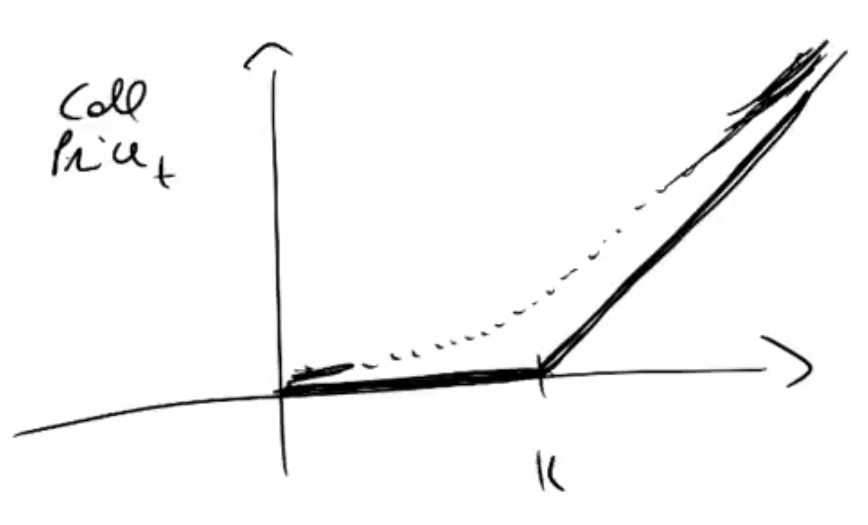
\includegraphics[scale=0.3]{fig/tmp/fig12.png}
    \caption{$\Phi(d_1)$ for call payoff.}
    \label{fig:priced}
\end{figure}
When we take its derivative with respect to $S$, i.e. the $\Delta$, we obtain the cumulative gaussian density (see Figure \ref{fig:delta}).
\begin{figure}[htp]
    \centering
    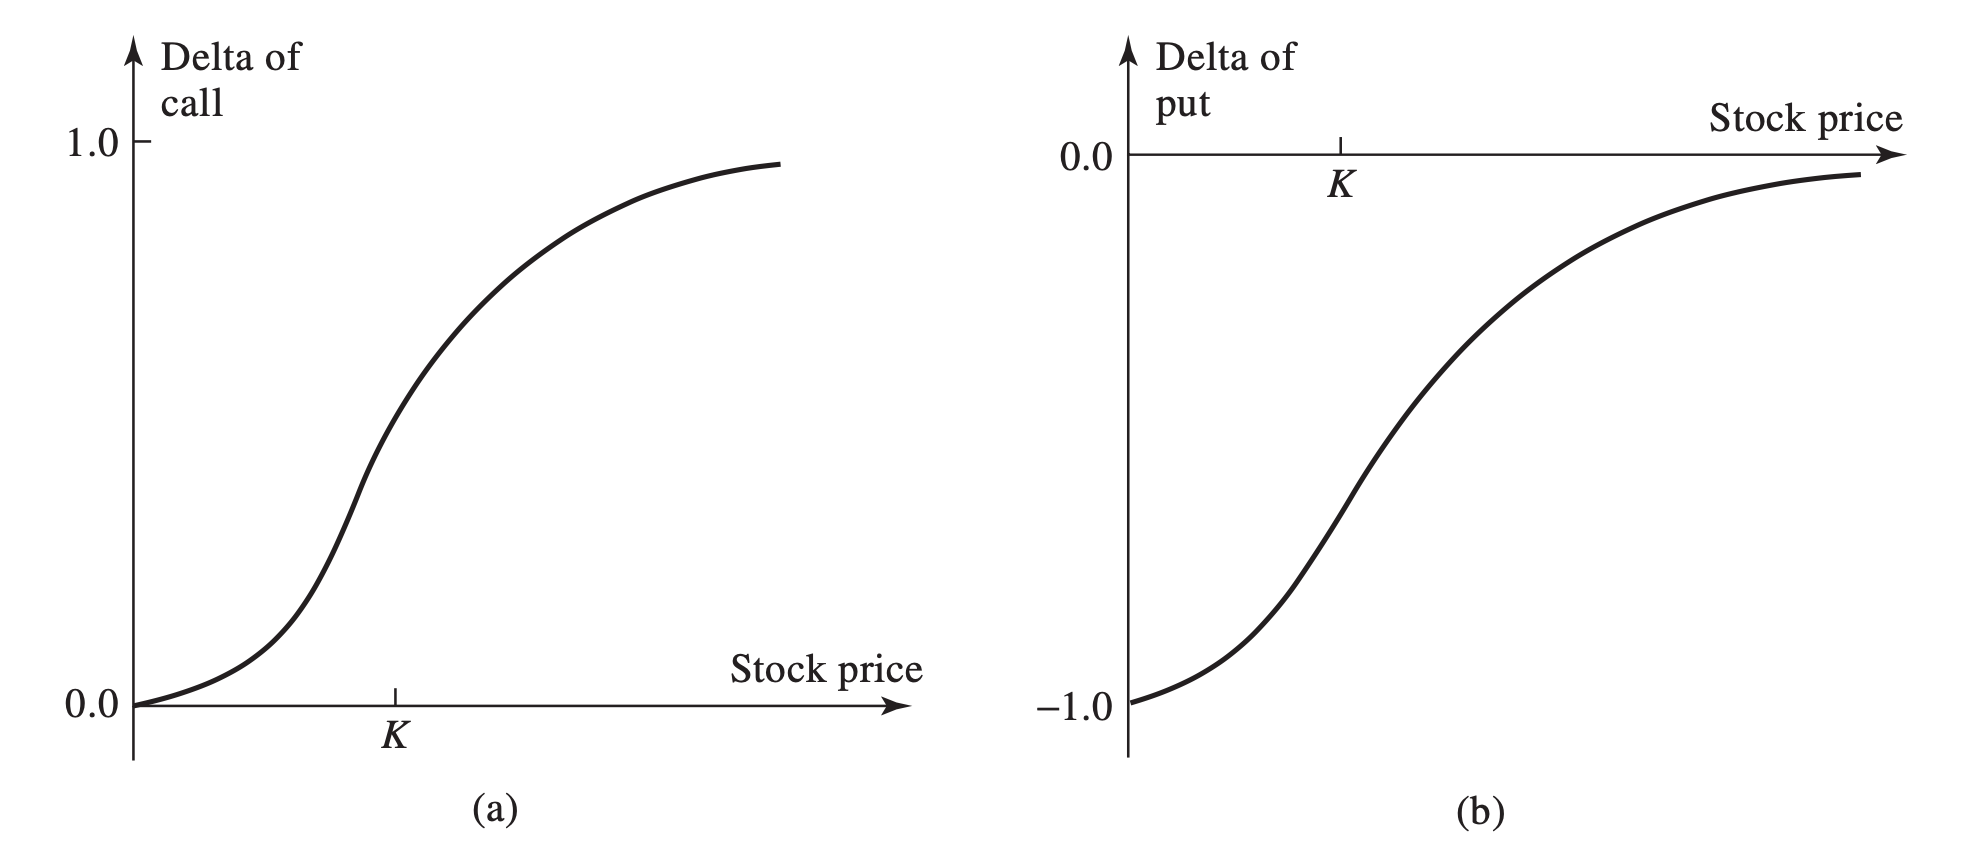
\includegraphics[scale=0.2]{fig/tmp/fig13.png}
    \caption{Variation of delta with stock price for (a) a call option and (b) a put option on a non-dividend-paying stock.}
    \label{fig:delta}
\end{figure}
The financial intuition is the following. When the underlying is less than the strike we are out of the money and there is no need to keep it in our portfolio. On the other hand, if the underlying is greater than the strike we are in the money and in order to construct the payoff for our long counterpart we have to hold a great amount of underlying (almost 1). The problem arises around the strike $K$, because for small fluctuations around $K$ there can be huge changes in the hedging portfolio.\\
So, hedging is more irregular than pricing. This is due to the fact that pricing involves an expectation, which is an integral that increases regularity. On the contrary, by deriving we loose regularity.\\
\\

\lesson{13}{09/04/2020} Now we would like to know the frequency at which we have to re-balance our portfolio in order to follow the fluctuations of the underlying. This is given by the Greek $\Gamma$.

\subsection{Gamma} % riascolta se hai tempo
The gamma ($\Gamma$) of a portfolio of options on an underlying asset is the rate of change of the portfolio's delta with respect to the price of the underlying asset. It is the second partial derivative of the portfolio with respect to asset price:
\begin{equation}
    \Gamma = \pdv[2]{price}{S} = \pdv{\Delta}{S} = \dfrac{1}{S\sigma\sqrt{T-t}}\dfrac{e^{-\frac{d_1}{2}}}{\sqrt{2\pi}}.
\end{equation}
If gamma is small, the delta changes slowly and adjustments to keep a portfolio delta-neutral need to be made only relatively infrequently. If gamma is highly negative or highly positive, the delta is very sensitive to the price of the underlying asset and it is quite risky to leave a delta-neutral portfolio unchanged for any length of time.
\begin{figure}[htp]
    \centering
    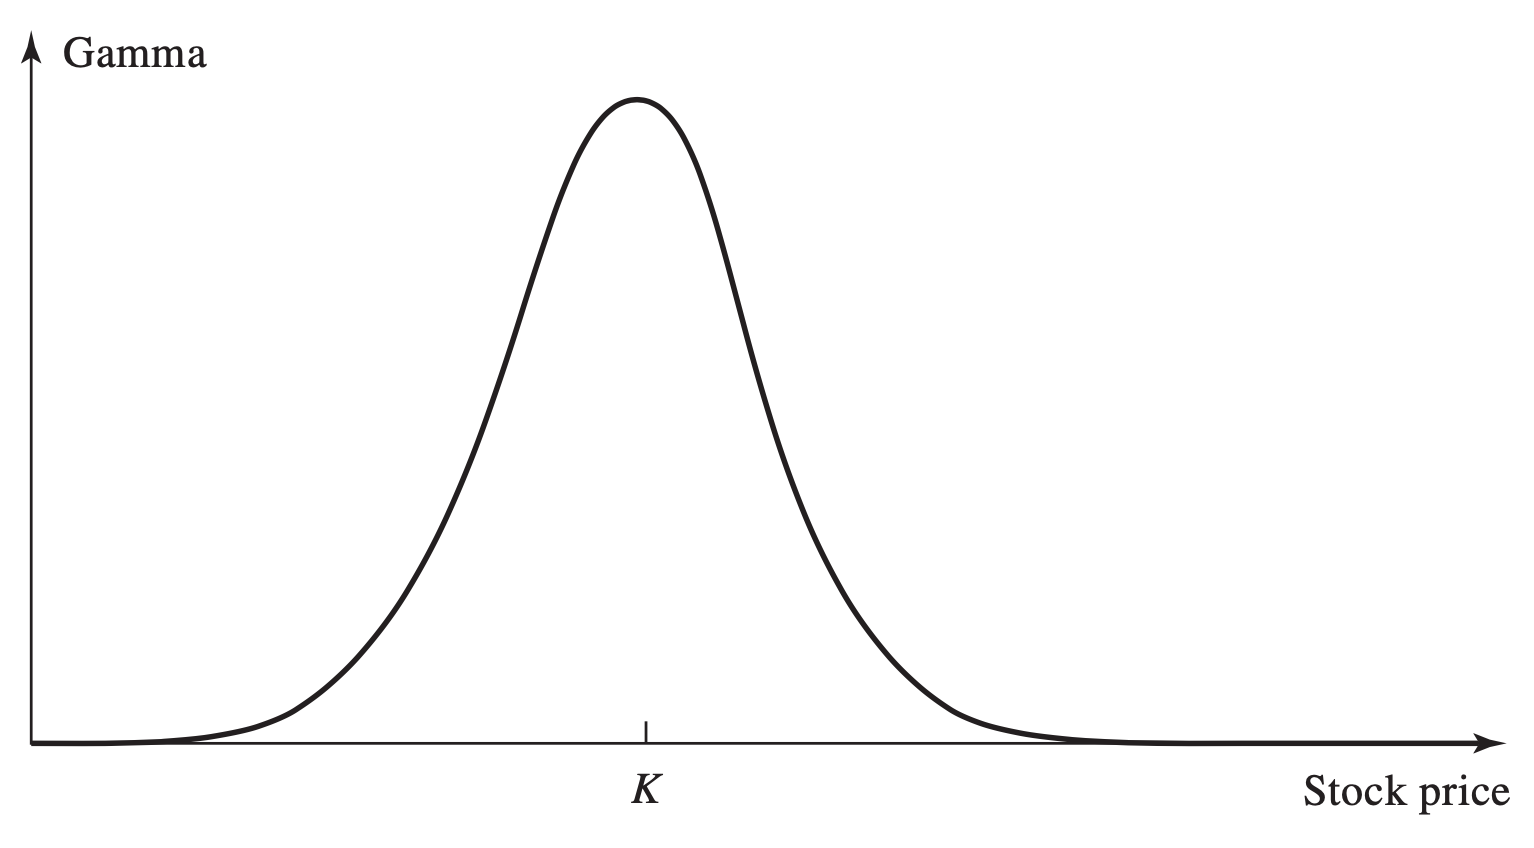
\includegraphics[scale=0.2]{fig/tmp/fig14.png}
    \caption{Variation of gamma with stock price for an option.}
    \label{fig:gamma}
\end{figure}

\subsection{Rho}
The rho of a portfolio of options is the rate of change of the value of the portfolio with respect to the interest rate:
\begin{equation}
    \rho = \pdv{price}{r} = K(T-t)e^{-r(T-t)}\Phi(d_2).
\end{equation}
It measures the sensitivity of the value of a portfolio to a change in the interest rate when all else remains the same. Notice that it is not normalized as the delta.
\begin{figure}[htp]
    \centering
    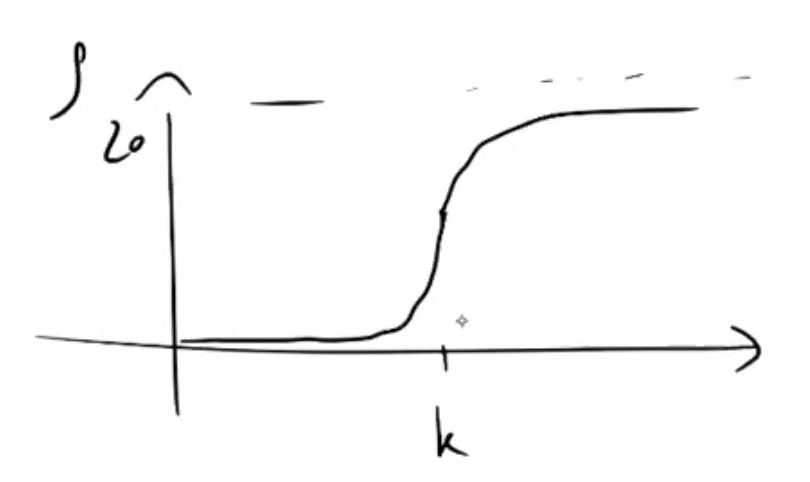
\includegraphics[scale=0.3]{fig/tmp/fig15.png}
    \caption{Variation of rho with stock price for an option.}
    \label{fig:rho}
\end{figure}
\newline Its interpretation is that if we are far from the strike, a bias in the estimation of the interest rate is not a problem. Conversely, if we are around the strike a small bias in the estimation of the interest rate results in a huge change in the price.

\subsection{Theta}
The theta ($\Theta$) of a portfolio of options is the rate of change of the value of the portfolio with respect to the passage of time with all else remaining the same. Theta is sometimes referred to as the \emph{time decay} of the portfolio.
\begin{equation}
    \Theta = \pdv{price}{t} = \dfrac{-S\sigma e^{-\frac{d_1^2}{2}}}{4\sqrt{2\pi(T-t)}}-rKe^{-r(T-t)}\Phi(d_2).
\end{equation}
Theta is usually negative for an option. This is because, as time passes with all else remaining the same, the option tends to become less valuable (we loose the opportunity to get a greater payoff). The variation of $\Theta$ with stock price for a call option is shown in Figure \ref{fig:theta}.
\begin{figure}[htp]
    \centering
    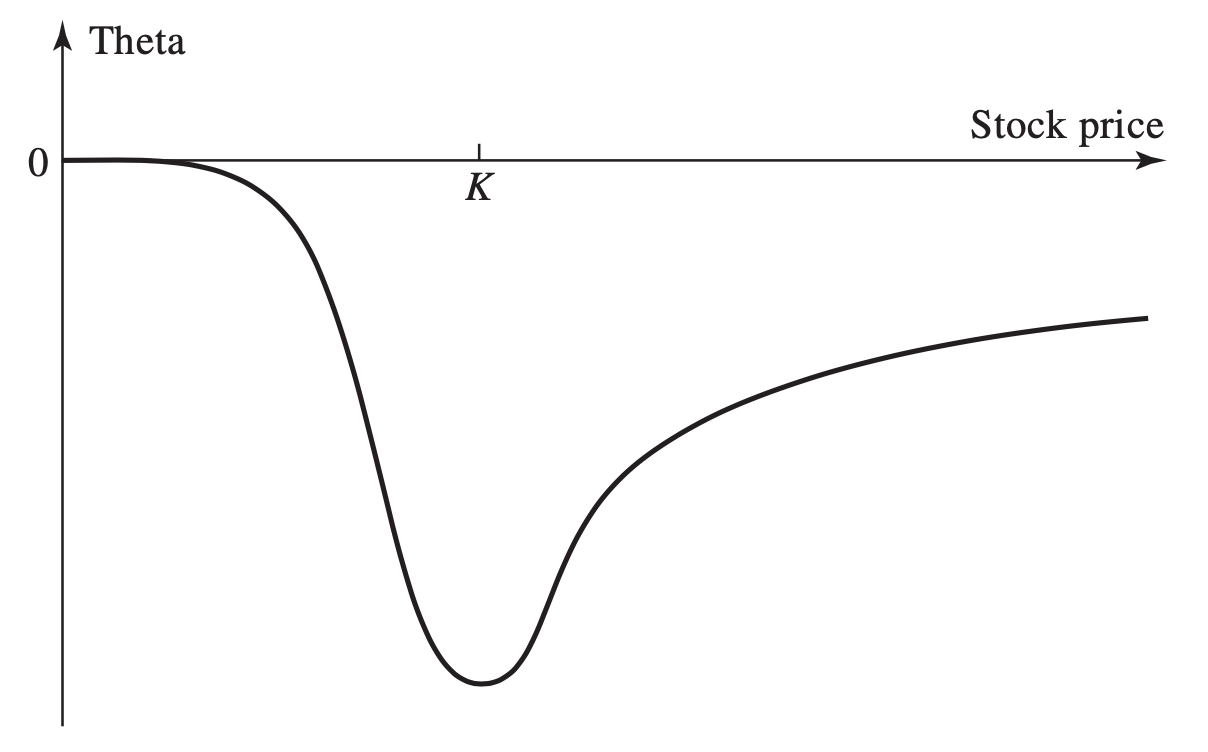
\includegraphics[scale=0.2]{fig/tmp/fig16.png}
    \caption{Variation of theta of a European call option with stock price.}
    \label{fig:theta}
\end{figure}
\newline When the stock price is very low, theta is close to zero. For an at-the-money call option, theta is large and negative. As the stock price becomes larger, theta tends to $-rKe^{-rT}$.

\subsection{Vega}
Up to now we have implicitly assumed that the volatility of the asset underlying a derivative is constant. In practice, volatilities change over time. This means that the value of a derivative is liable to change because of movements in volatility as well as because of changes in the asset price and the passage of time.\\
The vega of a portfolio of derivatives, $\mathcal{V}$, is the rate of change of the value of the portfolio with respect to the volatility of the underlying asset:
\begin{equation}
    \mathcal{V} = \pdv{price}{\sigma}.
\end{equation}
If vega is highly positive or highly negative, the portfolio’s value is very sensitive to small changes in volatility. If it is close to zero, volatility changes have relatively little impact on the value of the portfolio.
\begin{figure}[htp]
    \centering
    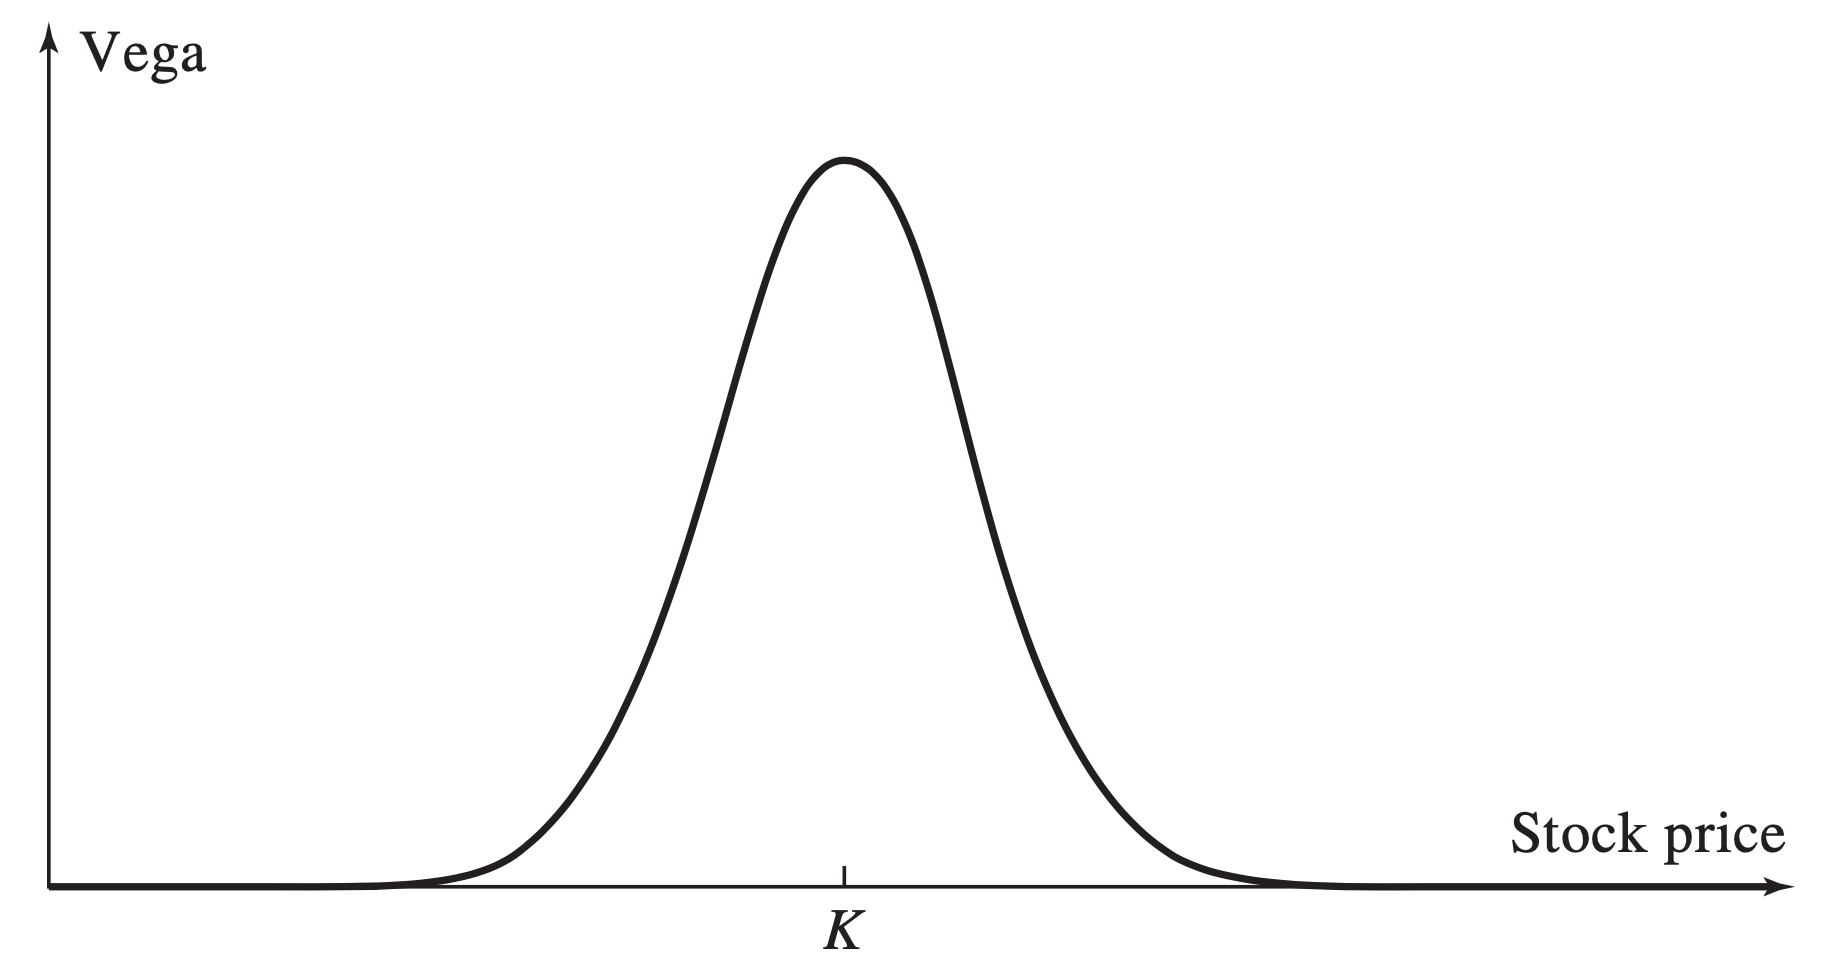
\includegraphics[scale=0.2]{fig/tmp/fig17.png}
    \caption{Variation of vega with stock price for an option.}
    \label{fig:vega}
\end{figure}
\newline The fact that $\mathcal{V}>0$ means that there is a monotone increasing relationship between price and volatility. In other words, the higher the volatility of the option, the higher the price of the option. We can exploit this relationship to invert the B\&S formula and find the volatility in terms of the price. Let us fix the maturity $T$ and suppose that we want to price a set of options indexed by different strikes $K_1,\dots,K_n$: $$B\&S(S,T-t,r,K_1,\sigma),\dots,B\&S(S,T-t,r,K_n,\sigma).$$
Now, if we consider the quoted prices
$$mkt(S,T-t,K_1),\dots,mkt(S,T-t,K_n)$$
we can look for the value of the volatility -- called \emph{implied volatility} -- to plug in the B\&S formula in order to obtain this prices. If the B\&S model is correct we should get always the same value of $\sigma_{imp}$, but indeed in practice we find non-constant values. This distortion is known as \emph{smile effect} and it is the proof that the B\&S model is not 100\% correct.
\begin{figure}[htp]
    \centering
    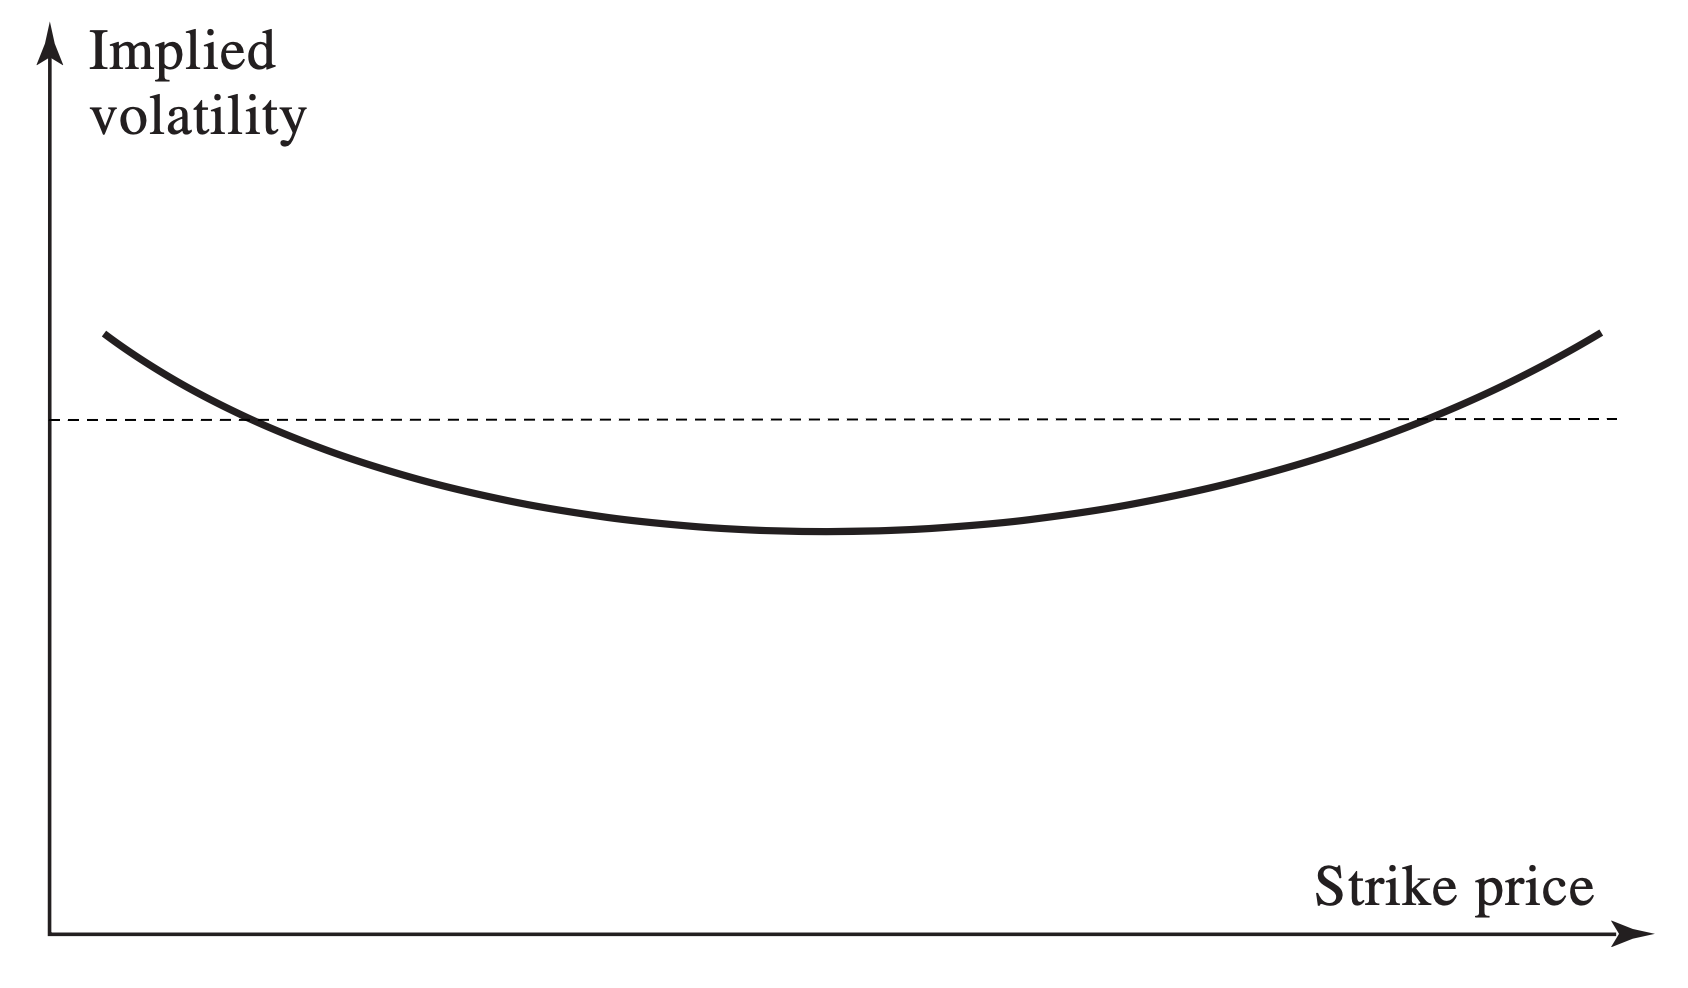
\includegraphics[scale=0.2]{fig/tmp/fig18.png}
    \caption{Smile effect.}
    \label{fig:smile}
\end{figure}
\newline However, the B\&S is very useful because it allows to quote the options not in dollars but in terms of the implied volatility.\\
The form of the smile is very important because it tells us how much the B\&S model is wrong. If the smile is flat it means that the B\&S model is not so wrong, while if it is more pronounced it means that it is dangerous to approximate prices using it.\\
The B\&S model is important also because in some contract there is not a quoted price, so it must be deduced.\\
If we consider different values of the maturity $T$ and we introduce the time to maturity as an additional dimension, we can find the so called \emph{implied volatility surface}. Typically, for short times to maturity the smile is very pronounced (the violation of the B\&S model is stronger) and for longer times to maturity the smile flattens (because of the central limit theorem).
\begin{figure}[htp]
    \centering
    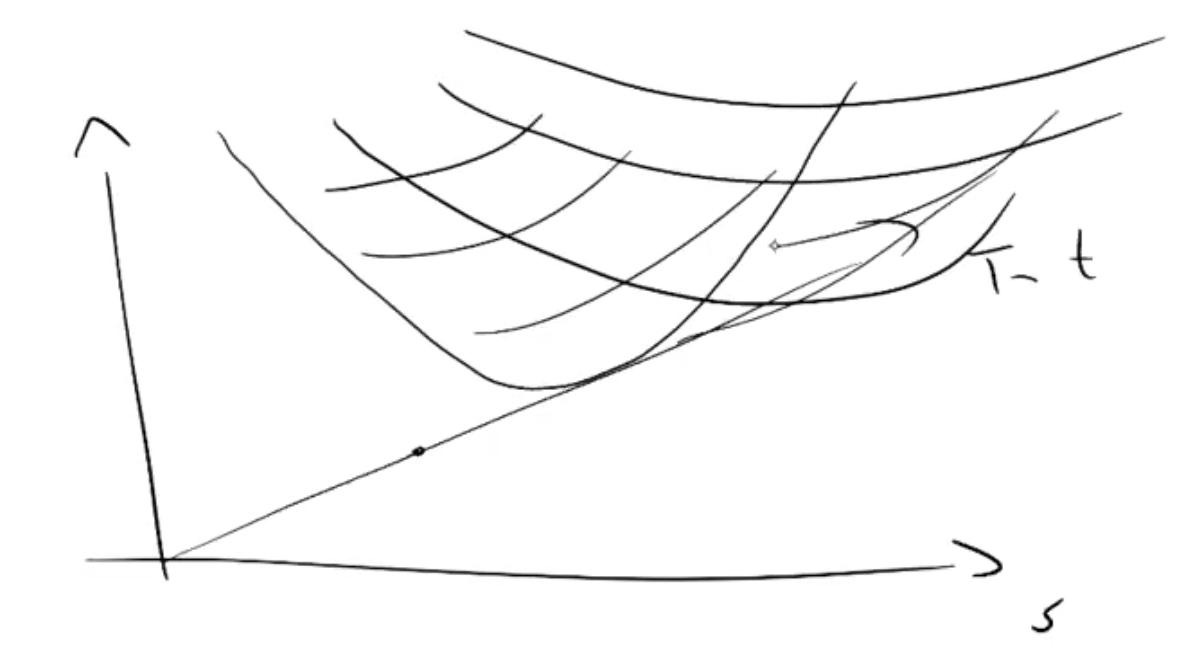
\includegraphics[scale=0.3]{fig/tmp/fig19.png}
    \caption{Implied volatility surface.}
    \label{fig:implvolsurf}
\end{figure}

\subsection{Put option pricing in the Black \& Scholes model}
From the put-call parity we have that:
\begin{align}
    \notag \text{Put}_t &= \call_t + Ke^{-r(T-t)} - S_t \\
    &=
    \notag S_t\Phi(d_1) - Ke^{-r(T-t)}\Phi(d_2) + Ke^{-r(T-t)} - S_t \\
    &=
    Ke^{-r(T-t)}\underbrace{(1-\Phi(d_2))}_{>0} - S_t\underbrace{(1-\Phi(d_1))}_{>0}.
\end{align}
Now we want to understand how to hedge a put option, in particular to find the Greeks. We have:
\begin{equation}
    \Delta^{\text{Put}} = \pdv{\text{Put}_t}{S} = \Phi(d_1)-1.
\end{equation}
In this case the delta of the put is always negative, as we can see in Figure \ref{fig:delta} (b). We also have
\begin{equation}
    \Gamma^{\text{Put}} = \Gamma^{\call},
\end{equation}
\begin{equation}\label{vegaput}
    \mathcal{V}^{\text{Put}} = \mathcal{V}^{\call}.
\end{equation}
Eq. \eqref{vegaput} is very important because it says that the price of the put is an increasing function of the corresponding volatility. This means that we can repeat the procedure of inverting the formula of the price of the put in terms of the volatility in order to get the quoted market price. Even in this case we will have the smile effect.\\
\textbf{What happens to the Greeks and to the price if there is an upward shift in the volatility?} Consider a call option. In any case there are the constraints to start from zero and to converge to the straight line $(S_t-K)^+$. Then we know that for higher volatility we will have higher prices. So, for $\sigma_2>\sigma_1$ the curve will stay above the original price.
The delta will change such that it will be convenient to buy the underlying earlier and to sell it immediately after the strike.
\begin{figure}[htp]
    \centering
    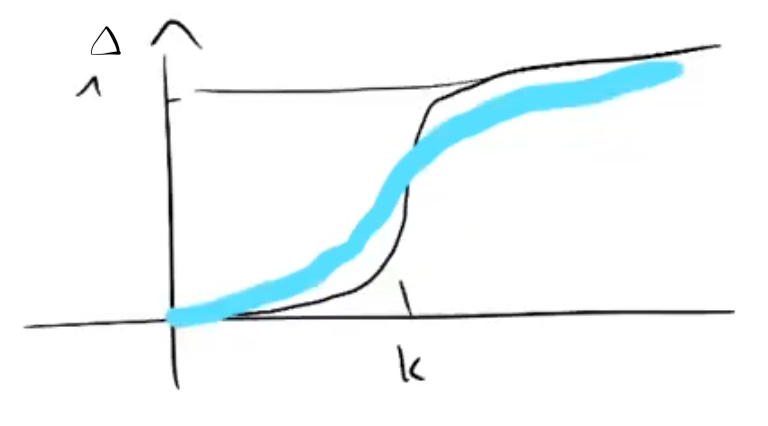
\includegraphics[scale=0.3]{fig/tmp/fig21.png}
    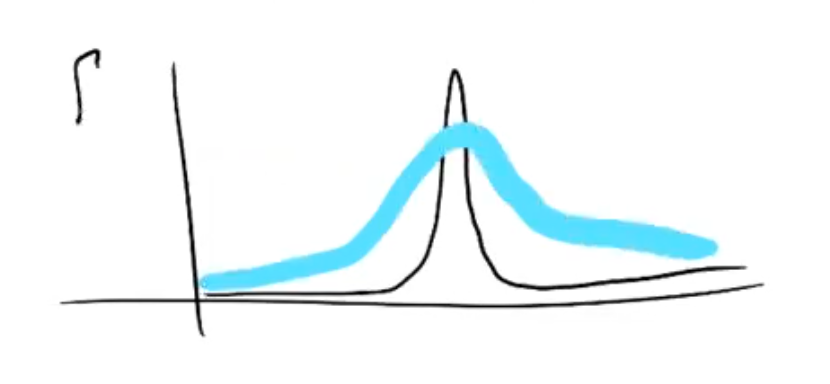
\includegraphics[scale=0.3]{fig/tmp/fig22.png}
    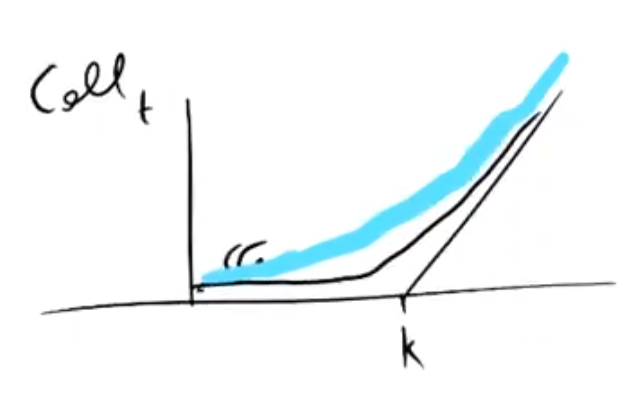
\includegraphics[scale=0.3]{fig/tmp/fig20.png}
    \caption{Delta, gamma and price of a call option for $\sigma_1$ (in black) and $\sigma_2>\sigma_1$ (in blue).}
    \label{fig:call2}
\end{figure}
If the gamma corresponding to $\sigma_1$ was like a Dirac delta, the one for $\sigma_2$ will be more spread out.\\
In other words, there is a smoothing effect both on the price and on the Greeks.

\section{Portfolio immunization}
We would like our portflio to be $\Delta$-neutral, i.e. we would like the global delta of our hedging strategy to match exactly the global delta of the corresponding portfolio derivatives. However, immediately after we balanced the portfolio, there can be a shock in the market. In other words, there is no guarantee for us to stay with the same hedging portfolio for too long. In order to stay safe for a while we need our portfolio to be $\Gamma$-neutral, so that the re-balance frequency is low. Moreover, since the volatility is a crucial ingredient we would like our portfolio to be also $\mathcal{V}$-neutral.\\
For example, from the B\&S PDE
\begin{equation}
    \pdv{F}{t} + rS\pdv{F}{S} + \frac{1}{2}\sigma^2S^2\pdv[2]{F}{S} = rF
\end{equation}
we can replace the derivatives with the corresponding Greeks:
\begin{equation}
    \Theta + rS\Delta + \frac{1}{2}\sigma^2S^2 \Gamma = r\, price.
\end{equation}
For a $\Delta$-neutral portfolio ($\Delta = 0$) we have
\begin{equation}
    \Theta + \frac{1}{2}\sigma^2S^2 \Gamma = r\, price.
\end{equation}
From this equality we immediately understand that if $\Theta<0$ then $\Gamma>0$, which is true for \emph{vanilla options} (call/put). Conversely, if $\Gamma<0$ then $\Theta>0$, which typically happens to \emph{exotic options}. In order to understand what does it mean to have a $\Gamma<0$, let's start from the dynamics of the hedging portfolio:
\begin{equation}
    \dd price_t = \Theta\,\dd t + S\Delta\,\dd S + \frac{1}{2}\sigma^2\Gamma\,\dd S^2.
\end{equation}
Notice that this is a quadratic function of $\dd S$. If $\Gamma$ is positive it means that for large variations of the underlying -- i.e. shocks in the market -- there is no risk (the hedging portfolio leads to a positive P\&L\footnote{The \emph{profit and loss} (P\&L) statement is a financial statement that summarizes the revenues, costs, and expenses incurred during a specified period, usually a fiscal quarter or year. The P\&L statement is synonymous with the income statement. These records provide information about a company's ability or inability to generate profit by increasing revenue, reducing costs, or both.}), whereas for small variations we can incur in some potential risk (negative P\&L). If $\Gamma<0$ we have the converse: for small variations of the underlying there is no risk (positive P\&L) whereas for large variations we can incur in some risk (negative P\&L).
\begin{figure}[htp]
    \centering
    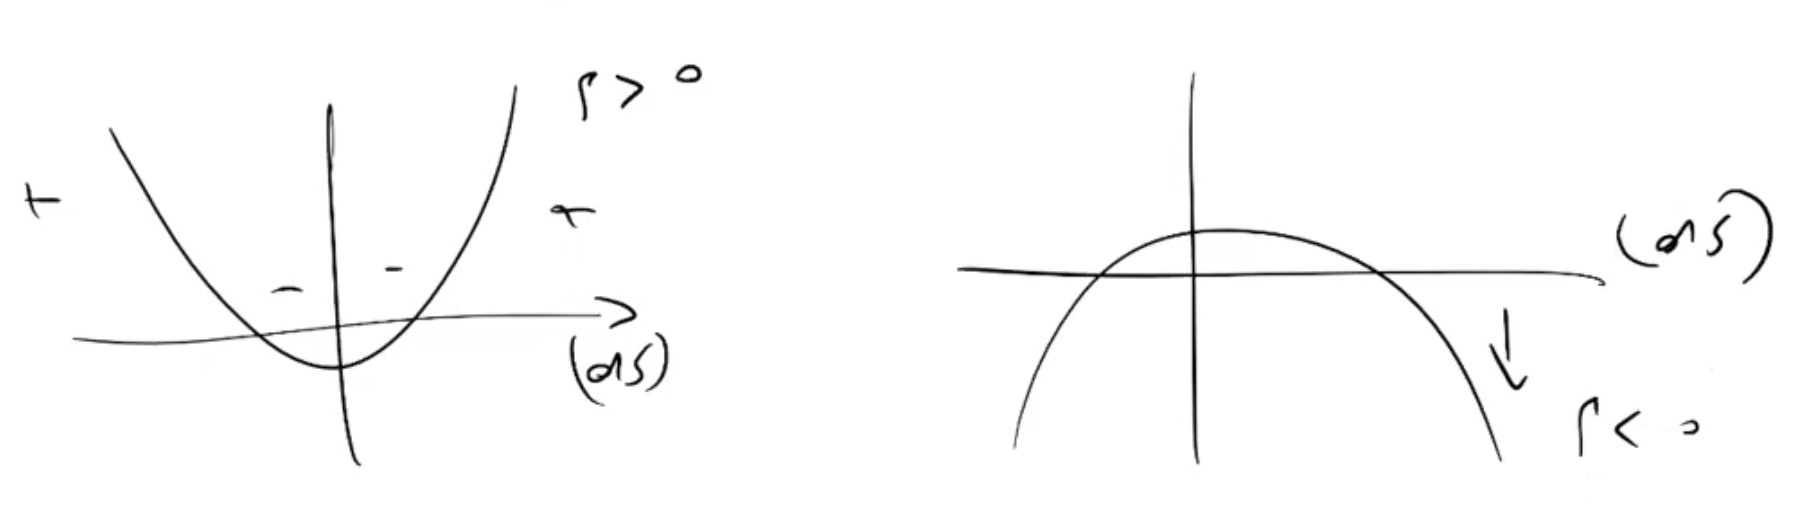
\includegraphics[scale=0.3]{fig/tmp/fig23.png}
    \caption{Hedging portfolio price for (a) $\Gamma>0$ and (b) $\Gamma<0$.}
    \label{fig:pnl}
\end{figure}
\newline Now let's construct an immune portfolio. At the end of the trading day the value of our portfolio is $V_t$ and the corresponding delta is $\Delta^V_t$. If $\Delta^V_t\gg0$ or $\Delta^V_t\ll0$ there is a mismatch between the behavior of what we are trying to hedge and our corresponding hedging strategy, known as \emph{delta risk}. We have to look for an instrument in the market that allows us to neutralize the global delta. There are two possibilities:
\begin{itemize}
    \item Buy/sell options (put, call, \dots). In the immunization we have to take into account their prices;
    \item Consider linear contracts (forward contract, futures, \dots). Since we do not have to pay in order to enter these contracts, these are cheaper strategies. These are delta-1 products, i.e. their delta is 1. In fact, if we consider as an example a long position in a forward contract, we have that the payoff is $S_T-K$ and according to the risk neutral methodology its price is
    \begin{align*}
        price_t^{\fwd} &= e^{r(T-t)}\mathbb{E}^\Qmeas[S_T-K]\\
        &=
        e^{rt}\mathbb{E}^\Qmeas[e^{-rT}S_T] - Ke^{r(T-t)} \\
        &=
        e^{rt}e^{-rt}S_t - Ke^{-r(T-t)} \\
        &=
        S_t - Ke^{-r(T-t)},
    \end{align*}
    so the delta is $\Delta^{\fwd}_t=1$.
\end{itemize}
Let's consider the situation in which $\Delta^V_t\ne0$ and we take a position in the forward market entering a contract with maturity $T$ and strike $K$, so that
\begin{equation}
    V^{tot}_t = V_t + \alpha\fwd(T,K),
\end{equation}
\begin{equation}
    \Delta_t^{tot} = \Delta_t^V + \alpha\Delta^{\fwd} = \Delta_t^V + \alpha\cdot 1.
\end{equation}
If we impose $\Delta_t^{tot}=0$ in the last equation we have that the number of forward contracts we have to include in our portfolio is
\begin{equation}
    \alpha = -\Delta^V_t.
\end{equation}
Furthermore, if we want also to neutralize the portfolio with respect to the \emph{gamma risk} (related to the frequency of re-balancing) then linear contracts are useless, because their second derivative with respect to $S$ is zero and so $\Gamma=0$. The idea is to take a position in the options market. The portfolio will be
\begin{equation}
    V^{tot}_t = V_t + \alpha\fwd_t + \beta \call(T,K)
\end{equation}
and we have to jointly impose the delta and gamma neutrality. In fact, if we take the previous $\Delta$-neutral portfolio and we impose the $\Gamma$-neutrality, the involved call option will have $\Delta^{\call}\ne0$ so the neutrality is destabilized. In other words, we have to solve
\begin{equation}
    \begin{cases}
    0 = \Delta^{tot}_t = \Delta_t^V + \alpha + \beta\Delta^{\call}_t \\
    0 = \Gamma^{tot}_t = \Gamma^V_t + 0 + \beta \Gamma^{\call}_t.
    \end{cases}
\end{equation}
If we want also vega-neutrality we have to consider a second option, different from the first (for example with different strike).

\section{Digital options}\lesson{14}{09/04/2020}
Digital options are related to a specific type of European options in which the payoff is either some fixed monetary amount or nothing at all:
\begin{equation}
    \pay_T = \mathds{1}_{S_T\ge K}
\end{equation}

\subsection{Pricing}
For pricing we can adapt the risk neutral methodology, but there is a much simpler way. In fact, we can write the call payoff as:
\begin{align}
    (S_T-K)^+ &= (S_T-K)\mathds{1}_{S_T\ge K} = S_T\mathds{1}_{S_T\ge K} - K\mathds{1}_{S_T\ge K}
\end{align}
So the price of the digital option payoff is:
\begin{align}
    \notag price^{DIG}_t &= e^{-r(T-t)}\expect_t[\mathds{1}_{S_T\ge K}] \\
    &=
    \notag e^{-r(T-t)}\Qmeas_t(S_T\ge K) \\
    &=
    e^{-r(T-t)}\Phi(d_2)
\end{align}
where $\Qmeas$ is the conditional risk neutral probability. So we only have to compute the gaussian CDF. The problems appear when we will consider the hedging: we saw that in the call option the payoff is continuous (it is the solution of a PDE) and differentiable. Here the payoff is even not continuous, so we expect additional irregularities in the Greeks. 

\subsection{Hedging}
Recall that 
\begin{equation*}
    \Phi(d_2) = \int^{d_2}_{-\infty} \dfrac{e^{-\frac{x^2}{2}}}{\sqrt{2\pi}}\,dx \qquad\Rightarrow\qquad \pdv{\Phi(d_2)}{S} = \dfrac{e^{-\frac{d_2^2}{2}}}{\sqrt{2\pi}}\dfrac{1}{S\sigma\sqrt{T-t}}
\end{equation*}
so the delta is
\begin{equation}
    \Delta^{DIG}_t = \dfrac{e^{-r(T-t)}e^{-\frac{d_2^2}{2}}}{\sqrt{2\pi}S\sigma\sqrt{T-t}}
\end{equation}
and in this case its shape is like a Dirac delta.
\begin{figure}[htp]
    \centering
    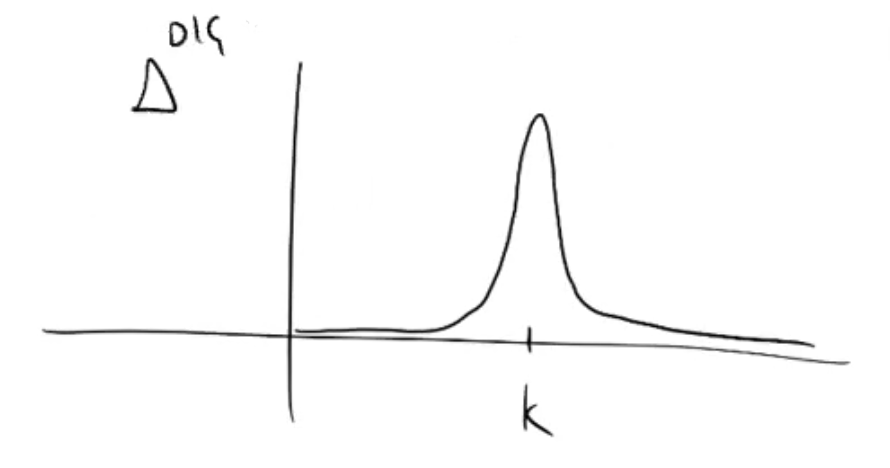
\includegraphics[scale=0.3]{fig/tmp/fig24.png}
    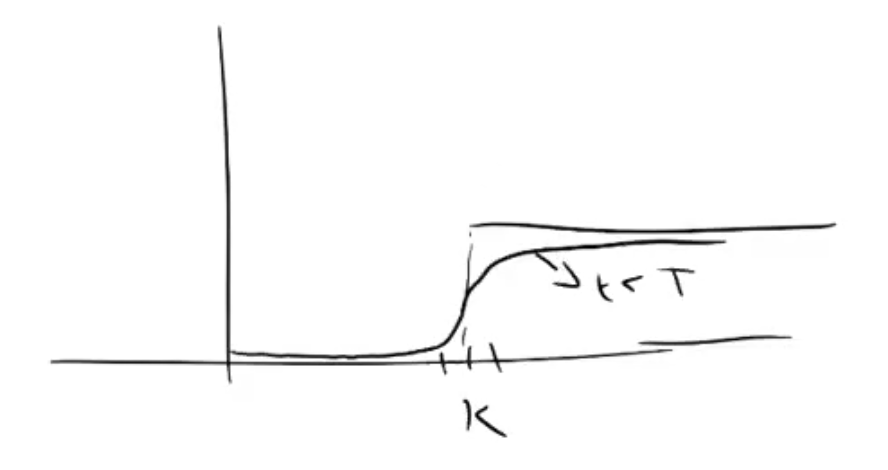
\includegraphics[scale=0.3]{fig/tmp/fig25.png}
    \caption{(a) Delta and (b) pricing function for the digital options.}
    \label{fig:digdelta}
\end{figure}
With such a delta, if the underlying fluctuates in a small interval around the strike it is impossible to hedge a digital option. In fact, the price function is such that it is impossible to buy or sell without incurring in a huge risk (in correspondence of the unitary jump). \\
Unfortunately, the traders' portfolios are typically full of digital options because they think in a myopic way: three years and three years plus a week are almost the same. So, if they have to match some conditions in a horizon of three years they look in the market for some products with maturity quite close to the one they have to hedge. But as time goes by the maturity approaches, and if for example we hedge with an option which maturity is a bit shorter there will remain a small additional increment of maturity (one week) in which we are uncovered (or in some other cases overcovered, i.e. we are over-hedging). The way traders hedge digital options is like a proxy, in the sense that instead of considering the true payoff of the option (the step function) they consider a combination of different options. For example, they consider a long call with strike $K_1$ and a short call with strike $K_2$ (Figure \ref{fig:dighedge}). This combination is called \emph{bull spread} (we have limited profits but limited losses).
\begin{figure}[htp]
    \centering
    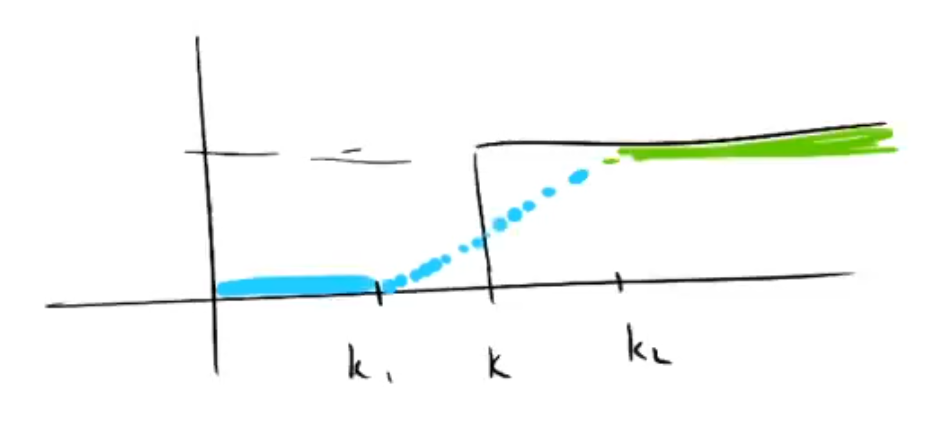
\includegraphics[scale=0.3]{fig/tmp/fig26.png}
    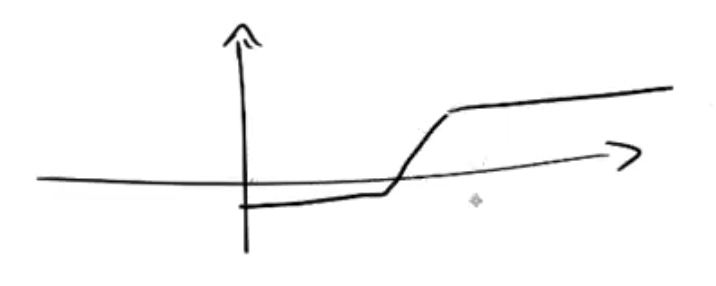
\includegraphics[scale=0.3]{fig/tmp/fig27.png}
    \caption{Bull spread.}
    \label{fig:dighedge}
\end{figure}
Now, let's consider the gamma:
\begin{equation}
    \Gamma^{DIG} = \pdv{\Delta^{DIG}}{S} 
\end{equation}
The explicit expression is not very interesting, the important thing is that it can be both positive or negative. If gamma is negative there is the possibility to incur in very heavy losses for large fluctuations of the underlying. This is an example of \emph{exotic options}, because it is very difficult to hedge and it has a potential negative gamma.
\begin{example}{}{}{}
    Consider the following payoff:
    \begin{equation}
        \pay_T = \begin{cases}
        -c_1 & S_T \in [0,K_1) \\
        S_T - K_1 - c_1 & S_T \in [K_1,K_2) \\
        K_3 - S_T - c_2 & S_T \in [K_2,K_3) \\
        -c_2 & S_T \ge K_3
        \end{cases}
    \end{equation}
    where $0<c_1<c_2$ and $0<K_1<K_2<K_3$. 
    \begin{enumerate}
        \item How can we price a product which leads to this payoff?
        \item Which is the form of delta and gamma?
        \item Show how the price changes for an upward shift of the volatility $\sigma_1\to\sigma_2>\sigma_1$.
    \end{enumerate}
    \textbf{Solution.} 1. First, let's visualize the payoff function.
    \begin{center}
        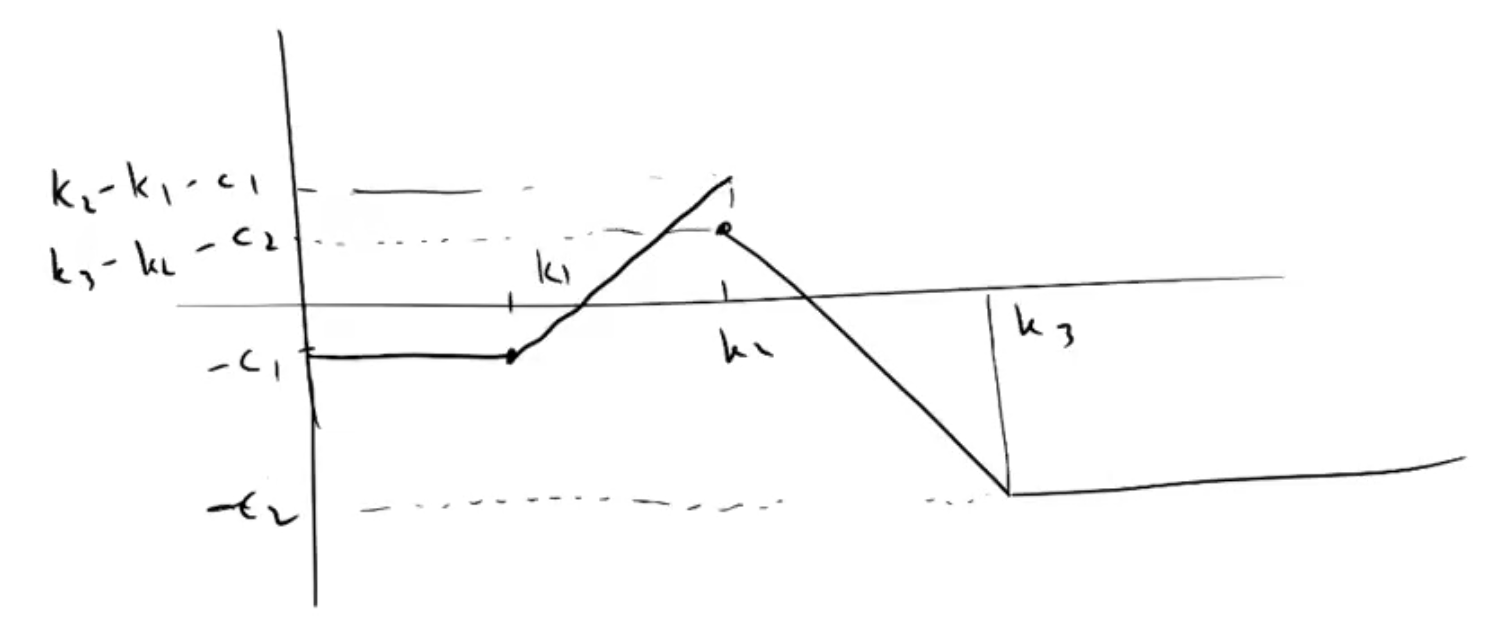
\includegraphics[scale=0.3]{fig/tmp/fig28.png}
    \end{center}
    In principle, we can always write the price as the discounted value of the risk neutral expectation of the payoff:
    \begin{align}
        \notag price_t(\pay_T) &= e^{-r(T-t)}\expect_t[\pay_T] \\
        &=
        e^{-r(T-t)}\left(\int_{-\infty}^{K_1}+\int_{K_1}^{K_2}+\int_{K_2}^{K_3}+\int_{K_3}^{+\infty}\right)
    \end{align}
    However, we would like to avoid brute force integration. Instead, we would like to write this expression in terms of some building blocks we already know how to price. We can start from the left or from the right. If we start from the left, the idea is to start with some product and add something else such that what is on the left remains unchanged and in case of need we can change what is in the right. But we know something that leaves the left unchanged: the call option. In fact, when the underlying is smaller than the strike, the call option has no effect. If we start from the right, the opposite holds and we can use put options.\\
    Let's start from the left. The payoff decomposition is the following:
    \begin{itemize}
        \item The payoff starts from $-c_1$ and it is constant till $K_1$. In order to have a straight line with slope $+1$ we consider a long position in a call option with strike $K_1$:
        \begin{equation*}
            \pay_T = -c_1 + (S_T+K_1)^+ +\dots
        \end{equation*}
        \item Now, in order to change the slope from $-1$ to 1 we take two short positions in a call with strike $K_2$:
        \begin{equation*}
            \pay_T = -c_1 + (S_T-K_1)^+ - 2(S_T-K_2)^+ + \dots
        \end{equation*}
        and in order to have the discontinuity in $K_2$ we translate downward the payoff by taking a number of short positions in a digital option equal to the size of the step:
        \begin{align*}
            \pay_T &= -c_1 + (S_T-K_1)^+ - 2(S_T-K_2)^+ - \\ 
            &\qquad 
            -(K_2-K_1-c_1-(K_3-K_2-c_2))\mathds{1}_{S_T\ge K_2} + \dots
        \end{align*}
        \item Now at $K_3$ we change the slope from $-1$ to 0 by taking a long position in a call with strike $K_3$:
        \begin{align}
            \notag \pay_T &= -c_1 + (S_T-K_1)^+ - 2(S_T-K_2)^+ - \\ 
            &\qquad 
            -(K_2-K_1-c_1-(K_3-K_2-c_2))\mathds{1}_{S_T\ge K_2} + (S_T-K_3)^+
        \end{align}
    \end{itemize}
    The corresponding price of this payoff is:
    \begin{align} %34:00
        \notag price_t(\pay_T) &= -c_1e^{-r(T-t)} + S_t\Phi(d_1^{K_1}) - e^{-r(T-t)}K_1\Phi(d_2^{K_1}) - \\
        &\qquad
        \notag - 2(S_t\Phi(d_1^{K_2})-e^{-r(T-t)}K_2\Phi(d_2^{K_2})) - \\
        &\qquad
        \notag - (2K_2-K_1-K_3-c_1+c_2)e^{-r(T-t)}\Phi(d_2^{K_2}) + \\
        &\qquad
        + S_t\Phi(d_1^{K_3}) - e^{-r(T-t)}K_3\Phi(d_2^{K_3})
    \end{align}
    where
    \begin{equation}
        d_1^{K_i} = \dfrac{\ln\frac{S}{K_i}+\left(r+\frac{\sigma^2}{2}\right)(T-t)}{\sigma\sqrt{T-t}}, \qquad i = 1,2,3
    \end{equation}
    2. The delta is given by the sum of the building blocks' deltas:
    \begin{align}
        \Delta_t = 0 + \Phi(d_1^{K_1}) - 2\Phi(d_1^{K_2}) - \Delta^{DIG, K_2} + \Phi(d_1^{K_3}) 
    \end{align}
    and the gamma is 
    \begin{equation}
        \Gamma_t = 0 + \dfrac{1}{S_t\sigma\sqrt{T-t}}\dfrac{e^{-\frac{d_1^{K_1}}{2}}}{\sqrt{2\pi}} - 2\dfrac{1}{S\sigma\sqrt{T-t}}\dfrac{e^{-\frac{d_1^{K_2}}{2}}}{\sqrt{2\pi}} - \Gamma^{DIG,K_2} + \dfrac{1}{S_t\sigma\sqrt{T-t}}\dfrac{e^{-\frac{d_1^{K_3}}{2}}}{\sqrt{2\pi}}
    \end{equation}
    3. If the volatility is $\sigma_2>\sigma_1$ the pricing function will be smoother. %fine parte 1
    \begin{center}
        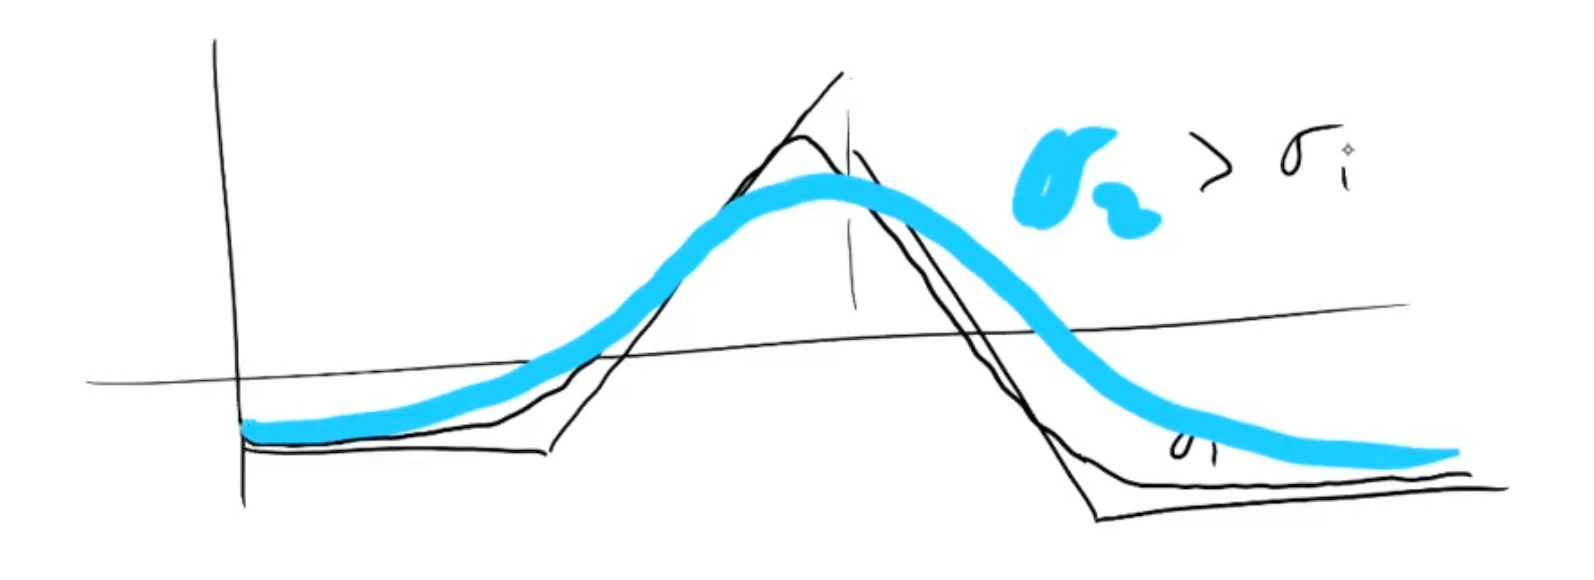
\includegraphics[scale=0.3]{fig/tmp/fig29.png}
    \end{center} 
\end{example}

\section{Black \& Scholes model with continuous dividends}\label{B&Swithdividends}
In this section we consider the case when dividends are paid out continuously in time. As usual $S_t$ denotes the price of the stock at time $t$, and by 
\begin{equation}
    D(t) = \int^t_0 \Tilde{\delta}_s \, \dd s    
\end{equation}{}
we denote the cumulative dividends over the interval $[0,t]$. $\Tilde{\delta}$ is the rate of dividends. Put in differential form, this means that over the infinitesimal interval $(t, t + \dd t]$ the holder of the stock receives the amount $\dd D(t) = D(t + \dd t) - D(t)$.\\
The starting point is the B\&S formula:
\begin{equation}
    \dfrac{\dd S}{S} = \mu\dd t + \sigma \dd W^{\Pmeas} 
\end{equation}
where $\Pmeas$ is the historical probability measure. We still don't know which is the risk neutral probability measure because here the price of the asset changes differently according to the fact that some dividends are delivered or not. So, in order to find the risk neutral measure $\Qmeas$ we have to start from the beginning.\\
We define our portfolio as:
\begin{equation}
    V_t = h_t\cdot S_t, \qquad S_t = \binom{S_t}{e^{rt}}
\end{equation}
The old portfolio (before dividends) has value $h(t-\Delta t)S(t)$ and if at time $t$ there is a delivery of some dividends such that we get $h(t-\Delta t)(D(t)-D(t-\Delta t))$. So, the budget equation is given by:
\begin{equation}
    h(t-\Delta t)S(t) + h(t-\Delta t)(D(t)-D(t-\Delta t)) = h(t)S(t) + c(t)\Delta t
\end{equation}
Now, if we add and subtract $S(t-\Delta t)\Delta h(t)$ we end up with:
\begin{align}
    \notag\dd V_t &= h(t)\dd S_t + h(t)\dd D_t - c(t)\dd t \\
    &=
    h(t)(\dd S_t + \dd D_t) - c(t)\dd t 
\end{align}
In the presence of dividends, the self financing condition involves a \emph{gain process}, because in addition to the price we get something more, i.e. the dividends (which can be seen as an incoming salary). Since $\dd D(t) = D(t + \dd t) - D(t)$ is a forward increment we can use Itô's formula. Now, under the measure $\Qmeas$, we want the discounted asset with the additional presence of the future value of the future streams of dividends to be a martingale: 
\begin{equation}
    S_te^{-rt} + \int_0^t e^{-rs}\dd D_s
\end{equation}
This process is called \emph{normalized gain process}. \\
Now we look for the pricing PDE. Starting from the dynamics of our portfolio:
\begin{equation}
    \begin{cases}
    \dd V = h \dd S + h \dd D + 0 \\
    V_T = \pay_T = F(S_T,T)
    \end{cases}
\end{equation}
where the 0 means no consumption, we have
\begin{equation}\label{hsd}
    h_t \dd S_t + h_t \dd D_t = \pdv{F}{t}\dd t + \pdv{F}{S}\dd S + \dfrac{1}{2}\sigma^2S_t^2\pdv[2]{F}{S}\dd t
\end{equation}
Recall that 
\begin{equation}
    h = \binom{\alpha}{\beta}, \qquad S_t = \binom{S}{e^{rt}}, \qquad D = \binom{\int^t_0\Tilde{\delta}_s\,\dd s}{0}
\end{equation}
where the second element of $D$ is zero because there are no dividends in the riskless asset. Substituting in \eqref{hsd} we have:
\begin{align}\label{ll}
    \notag\hlc{mypink}{\alpha S(\mu\dd t + \sigma\dd W^{\Pmeas})}+\beta re^{rt}\dd t + \alpha\Tilde{\delta}_t\dd t =\, &\pdv{F}{t}\dd t + \hlc{mypink}{\pdv{F}{S}S(\mu\dd t + \sigma\dd W^{\Pmeas})} + \\
    &+ \dfrac{1}{2}\sigma^2S_t^2\pdv[2]{F}{S}\dd t
\end{align}
Comparing the pink boxes, we see that, even in presence of dividends, $\alpha$ is still given by
\begin{equation}\label{a}
    \alpha = \pdv{F}{S} = \Delta_t 
\end{equation}
Substituting \eqref{a} in \eqref{ll}, the two pink terms cancel out and we get the following PDE:
\begin{equation}
    \pdv{F}{t}\dd t + rS\pdv{F}{S} + \dfrac{1}{2}\sigma^2S_t^2\pdv[2]{F}{S} - \Tilde{\delta}\pdv{F}{S} - rF = 0 
\end{equation}
Financially speaking, it is not reasonable that $\Tilde{\delta}$ is constant because the rate of dividends should depend on the value of the asset. The typical assumption is that $\delta_s$ is given by a constant $q$ times the value of the asset at time $t$:
\begin{equation}
    \Tilde{\delta}_s = qS_t 
\end{equation}
In this case we speak about \emph{proportional dividends}, and the corresponding PDE reads:
\begin{equation}
    \begin{cases}
    \pdv{F}{t}\dd t + (r-q)S\pdv{F}{S} + \dfrac{1}{2}\sigma^2S_t^2\pdv[2]{F}{S} - rF = 0 \\
    F(S_T,T) = \pay_T
    \end{cases}
\end{equation} 
Now we apply the Feynman-Kac methodology in order to say that if $F$ is a solution of this PDE then there exist a probability space and a probability measure $\Qmeas^q$ under which we can define the B\&S equation
\begin{equation}
    \dfrac{\dd S}{S} = (r-q)\dd t + \sigma \dd W^{\Qmeas^q} 
\end{equation}
Such solution of the PDE can be written as 
\begin{equation}
    F(S_t,t) = e^{-r(T-t)}\mathbb{E}^{\Qmeas^q}_t[\pay_T]
\end{equation}
Now, recall that $S_t$ is the solution of the geometric Brownian motion equation. In presence of dividends we have:
\begin{align}
    S_t &= S_0e^{\left(r-q-\frac{1}{2}\sigma^2\right)T+\sigma W_T^{\Qmeas^q}} \\
    &=
    (S_0e^{-qT})e^{\left(r-\frac{1}{2}\sigma^2\right)T+\sigma W_T^{\Qmeas^q}}
\end{align}
Notice that since we can write $(S_0e^{-qT})$ as a new initial value, we have that
\begin{equation}
    F_q(S_t,t) = F_0(S_te^{-q( T-t)})
\end{equation}
Now we are ready to write the Black \& Scholes formula in presence of dividends:
\begin{equation}
    price^{\call}(t,T,S_t,K,\sigma,r,q) = S_te^{-q( T-t)}\Phi(d_1)-Ke^{-r(T-t)}\Phi(d_2)
\end{equation}
with 
\begin{equation}
    d_1 = \dfrac{\ln\frac{S_te^{-q(T-t)}}{K}+\left(r+\frac{1}{2}\sigma^2\right)(T-t)}{\sigma\sqrt{T-t}} = \dfrac{\ln\frac{S_t}{K}+\left(r-q+\frac{1}{2}\sigma^2\right)(T-t)}{\sigma\sqrt{T-t}}
\end{equation}
\begin{equation}
    d_2 = d_1 - \sigma\sqrt{T-t}
\end{equation}
Using the put-call parity we immediately get the price of a put option.
\section{Multi-dimensional market}\lesson{15}{10/04/2020} % Bjork ch. 13
We assume that we have $n$ a priori given risky assets (“stocks”) with price processes $S_1(t),\dots,S_n(t)$ and a riskless asset with price process $S_0(t)$, which evolves according to a certain interest rate:
\begin{equation}
    \dfrac{\dd S_0(t)}{S_0(t)} = r_t\,\dd t
\end{equation}
The entire asset price vector is denoted by $S(t)$, and in matrix notation we will write it as a column vector:
\begin{equation}
    S(t) = (S_0(t), S_1(t),\dots,S_n(t))^T
\end{equation}
According to the B\&S formula, the singular risky asset dynamic follows the equation:
\begin{equation}
    \dfrac{\dd S_i(t)}{S_i(t)} = \mu_i\,\dd t + \sum^d_{j=1}\sigma_{ij}\,\dd W_j^{\Pmeas}(t)
\end{equation}
where $W^{\Pmeas}(t)\in\mathbb{R}^d$ is a standard Brownian motion, i.e. $W_i\indep W_j$ $\forall i\ne j$. Here we assume that $r_t, \mu_i$ and $\sigma_{ij}$ are adapted processes to the corresponding filtration (that we assume generated by the Brownian motion itself). Notice that the number $n$ of assets is not necessarily equal to the Brownian motions $d$ driving the assets, so $\sigma:\mathbb{R}^d\to\mathbb{R}^n$.\\
Let's give an intuition of what we want to do. Consider, for example, a two assets model ($n=2$), that is a model with two risky assets and one riskless asset. Assume that $\mu,\sigma$ and $r$ are constant. The evolution of the risky assets is
\begin{align}\label{bm}
    \dfrac{\dd S_1(t)}{S_1(t)} &= \mu_1\,\dd t + \sum^d_{j=1}\sigma_{1j}\,\dd W_j^{\Pmeas}(t) \\
    \dfrac{\dd S_2(t)}{S_2(t)} &= \mu_2\,\dd t + \sum^d_{j=1}\sigma_{2j}\,\dd W_j^{\Pmeas}(t)
\end{align}
If $d=1$ both assets are driven by the same Brownian motion, i.e. they are perfectly correlated (the source of randomness is the same). However, if the drifts are different, there can be a potential presence of an arbitrage opportunity (we can discount with respect to the volatility and the corresponding rate of growth may be different). If $d>2$ we can always reduce the number of Brownian motions by normalizing the noise, in fact a linear combination of three Brownian motions can always be written as a combination or two or one Brownian motion(s).
\begin{example}{How to reduce the number of Brownian motions}{}{}
    If $d=2$, eq. \eqref{bm} become:
    \begin{align}
        \dfrac{\dd S_1(t)}{S_1(t)} &= \mu_1\,\dd t + \sigma_{11}\,\dd W_1^{\Pmeas}(t) + \sigma_{12}\,\dd W_2^{\Pmeas}(t) \\
        &=
        \mu_1\,\dd t + \sqrt{\sigma_{11}^2 + \sigma_{12}^2}\,\dd \widetilde{W}(t)
    \end{align}
    where 
    \begin{equation}
        \widetilde{W} = \dfrac{1}{\sqrt{\sigma_{11}^2 + \sigma_{12}^2}}(\sigma_{11}W_1^{\Pmeas}(t) + \sigma_{12}W_2^{\Pmeas}(t))
    \end{equation}
    The quadratic variation of $\Tilde{W}$ is
    \begin{equation}
        \expval{\widetilde{W}}_t = t 
    \end{equation}
    and this is the proof that $\Tilde{W}$ is a true Brownian motion. So, one Brownian motion for process is enough.
\end{example}
So, we can write eq. \eqref{bm} as:
\begin{align}
    \dfrac{\dd S_1(t)}{S_1(t)} &= \mu_1\,\dd t + \sigma_{1}\,\dd W_1^{\Pmeas}(t) \\
    \dfrac{\dd S_2(t)}{S_2(t)} &= \mu_2\,\dd t + \sigma_{2}\,\dd W_2^{\Pmeas}(t)
\end{align}
We know that $\dd W_1^{\Pmeas}$ and $\dd W_2^{\Pmeas}$ are independent. This means that the two assets are independent, which is not a very realistic assumption -- statistically speaking. So, we have to introduce some kind of correlation.\\
Let's consider a triangular construction involving, asset after asset, a new Brownian motion:
\begin{align}
    \dfrac{\dd S_1(t)}{S_1(t)} &= \mu_1\,\dd t + \sigma_{1}\,\dd W_1^{\Pmeas}(t) \\
    \dfrac{\dd S_2(t)}{S_2(t)} &= \mu_2\,\dd t + \sigma_{2}\underbrace{(\rho\,\dd W_1^{\Pmeas}(t) + \sqrt{1-\rho^2}\,\dd W_2^{\Pmeas})}_{\expval{\cdot}_t=t} %\\
    %\dfrac{\dd S_3(t)}{S_3(t)} &= \mu_3\,\dd t + \sigma_{3}\underbrace{(??\,\dd W_1^{\Pmeas}(t) + ??\,\dd W_2^{\Pmeas} + ??\,\dd W_3^{\Pmeas}(t))}_{\expval{\cdot}_t=t}
\end{align}
where $\rho$ represents the correlation between the two Brownian motions (i.e. between the two assets). This approach has two advantages: first, there is the possibility to decompose the matrix $\sigma$ using the Cholesky decomposition\footnote{The Cholesky decomposition of a Hermitian positive-definite matrix $A$ is a decomposition of the form
$A=LL^*$ where $L$ is a lower triangular matrix with real and positive diagonal entries, and $L^*$ denotes the conjugate transpose of $L$. Every Hermitian positive-definite matrix (and thus also every real-valued symmetric positive-definite matrix) has a unique Cholesky decomposition.}; second, it allows to introduce additional assets without affecting the evolution of the previous assets.

\subsection{Absence of arbitrage}
Recall that the absence of arbitrage is related to the existence of a probability measure $\Qmeas$ under which all the assets are martingales:
\begin{equation*}
    S^i_t e^{-\int_0^t r_s\,\dd s} = \Qmeas-martingale
\end{equation*}
Recall also that we found that in order to go from the Brownian motion under the historical probability measure $\Pmeas$ to the one under the risk neutral probability measure $\Qmeas$ we just have to make a shift involving a finite variation process $\lambda\in\mathbb{R}^d$:
\begin{equation*}
    \dd W_t^{\Pmeas} \longrightarrow \dd W_t^{\Qmeas} + \lambda(t)\dd t
\end{equation*}
The change of measure is related to the Girsanov theorem through the Radon-Nikodym derivative:
\begin{equation}
    \eval{\dv{\mathbb{Q}}{\mathbb{P}}}_t = \exp\left(\int^t_0 \lambda_s^T\cdot\dd W_s^{\mathbb{P}}-\dfrac{1}{2}\int^t_0 \norm{\lambda_s}^2\,\dd s\right)
\end{equation}
The fact that
\begin{equation}\label{159}
    \mu + \sigma\lambda = (r,\dots,r)^T \in \mathbb{R}^n
\end{equation}
means that, after the change of measure, the drifts $\mu_i$ are transformed into the drifts which is equal to $r$ for all the components. $\mu$, $\sigma$, and $r$ are given a priori and we want to solve for $\lambda$. Thus, for each $t$ the $n$-dimensional vector $\mu(t)-r(t)$ must be in the image of the diffusion matrix $\sigma(t)$, so we have the following result.
\begin{proposition}
    A necessary condition for absence of arbitrage is that
    \begin{equation}
        \mu(t) - r(t) \in \Im{\sigma}
    \end{equation}
    with probability one for each $t$.
\end{proposition}
We then have the following central result.
\begin{proposition}
    The model is generically arbitrage free (arbitrage free for every (sufficiently integrable) choice of $\mu$) if and only if, for each $t\le T$ and $\Pmeas$-a.s., the mapping
    \begin{equation}
        \sigma: \mathbb{R}^d \to \mathbb{R}^n
    \end{equation}
    is surjective, i.e. if and only if the volatility matrix $\sigma(t)$ has rank $n$.
\end{proposition}
From this result it follows in particular that for absence of arbitrage we must in the generic case necessarily have $d\ge n$, i.e. we must have at least as many independent Wiener processes as we have risky assets (as we said before).

\subsection{Completeness}
We now go on to obtain conditions for the model to be complete, and in order to avoid pathological cases we assume that the model is generically arbitrage free. From the Second Fundamental Theorem \ref{secondfundth} we know that the model is complete if and only if the martingale measure is unique, so it is tempting to draw the conclusion that we have completeness if and only if equation \eqref{159} has a unique solution, i.e. if and only if the condition
\begin{equation}
    \ker(\sigma) = \{0\},
\end{equation}
is satisfied for all $t$ and with probability one. This is, however, not quite true and the reason is that, in case of a general filtered probability space, there is no guarantee that all equivalent measure transformations are of the Girsanov type above. In a general situation, where there are other sources of randomness beside the Wiener process $W$, the Girsanov transformation above will only change the measure for the Wiener process, but it will not affect the other processes. So, in the presence of jumps, we cannot replicate all the contingent claims.\\
In order to obtain sharp results we are therefore forced to make the assumption that all randomness in our model is generated by the Wiener process $W$. 
\begin{theorem}
    Assume that the model is generically arbitrage free and that the filtration $\mathcal{F}$ is defined by
    \begin{equation}
        \mathcal{F}_t = \mathcal{F}_t^W
    \end{equation}
    i.e. there are no jumps. Then, disregarding integrability problems, the market is complete if and only if $k = n$ and the volatility matrix $\sigma(t)$ is invertible, i.e. $\ker(\sigma) = \{0\}$, $\Pmeas$-a.s. for each $t\le T$.
\end{theorem}
\begin{proof}
    The martingale measure is unique if and only if the solution $\lambda$ of the “martingale measure equation” 
    \begin{equation*}
        \sigma\lambda=r-\mu
    \end{equation*}
    is unique, and this occurs if and only if $\sigma(t)$ is injective, which implies $d \le n$. But since we have assumed generic absence of arbitrage, we know that $n \ge d$ and that $\sigma(t)$ is surjective. Thus $d = n$ and $\sigma(t)$ is invertible. \\
    Alternatively, from the fact that $\Im{\sigma}=\mathbb{R}^n$ and $\Im{\sigma^T}=\mathbb{R}^d$ we have that
    \begin{equation*}
        \ker(\sigma) = (\Im{\sigma^T})^{\perp} = \{0\}
    \end{equation*}
    Thus $\sigma(t)$ is invertible and $d = n$.
\end{proof}
This theorem states that if we want completeness the number of Brownian motions must be equal to the number of assets. 

\subsection[Pricing]{The pricing problem with two risky assets in the Black \& Scholes model}
The dynamic of the assets under the neutral probability measure $\Qmeas$ is given by:
\begin{align}
    \dfrac{\dd S_1(t)}{S_1(t)} &= r\,\dd t + \sigma_{11}\,\dd W_1^{\Qmeas}(t) + \sigma_{12}\,\dd W_2^{\Qmeas}(t) \\
    \dfrac{\dd S_2(t)}{S_2(t)} &= r\,\dd t + \sigma_{21}\,\dd W_1^{\Qmeas}(t) + \sigma_{22}\,\dd W_2^{\Qmeas}(t)
\end{align}
where in the first asset we keep two Brownian motions in order to stick with the Bjork's book notation. \\
We want to price a contract which payoff $\Phi(S_1(t),S_2(t))$ depends on both assets $(S_1,S_2)$. According the risk neutral methodology, the price is given by the discounted value up to maturity of the conditional expected value of the payoff under the probability measure $\Qmeas$:
\begin{align}
    price_t &= e^{-r(T-t)}\expect_t[\Phi(S_1(t),S_2(t))] \\
    &= 
    F(t,S_1,S_2)
\end{align}
where in (a) we used the Feynman-Kac formula, as the payoff depends only on the terminal value of the underlying. $F$ solves the PDE: %S_1,S_2 = x_1,x_2
\begin{equation}\label{bspdee}
    \begin{cases}
    \pdv{F}{t} + r\left(x_1\pdv{F}{x_1} + x_2\pdv{F}{x_2}\right) + \dfrac{1}{2}\left(x_1^2\pdv[2]{F}{x_1}c_{11} + 2x_1x_2\pdv{F^2}{x_1x_2}c_{12} + x_2^2\pdv[2]{F}{x_2}c_{22}\right) - rF = 0 \\
    F(t,x_1,x_2) = \Phi(x_1(t),x_2(t))
    \end{cases}
\end{equation}
where from the Itô's formula we have the coefficients:
\begin{equation}
    \mqty(c_{11}&c_{12}\\c_{21}&c_{22}) = \sigma\sigma^T = \mqty(\sigma_{11}&\sigma_{12}\\\sigma_{21}&\sigma_{22})\mqty(\sigma_{11}&\sigma_{21}\\\sigma_{12}&\sigma_{22})
\end{equation}
\begin{example}{Exchange option}{}{}
    Consider an \emph{exchange option}, which gives the holder the right, but not the obligation, to exchange one $S_2$ share for one $S_1$ share at time $T$. Formally, this means that the payoff is
    \begin{equation}
        \Phi(S_1(T),S_2(T)) = (S_1(T)-S_2(T))^+
    \end{equation}
    which is similar to the call option payoff if we see $S_2$ as the strike. So, very naively, we can apply the B\&S formula to $S_1$ with strike $S_2$:
    \begin{equation}
        price_t^{EXC} = S_1(t)\mathcal{N}(d_1) + e^{-r(T-t)}S_2(T)\mathcal{N}(d_2)
    \end{equation}
    \textbf{This is wrong}, because, at time $t$, $S_2(T)$ is not a measurable quantity. Then we could adapt the formula by using $S_2(t)$, but this is an arbitrary choice. Moreover, if we use this adaptation on $d_1$ or $d_2$, we have (for example for $d_1$)
    \begin{equation}
        d_1 = \dfrac{\ln\frac{S_1(t)}{S_2(t)}+\left(r+\frac{1}{2}(\sigma_{11}^2 + \sigma_{12}^2)\right)(T-t)}{\sqrt{(\sigma_{11}^2 + \sigma_{12}^2)(T-t)}},
    \end{equation}
    so the price of this option will depend only on the volatility of the first asset (there is no $\sigma_{21}$ or $\sigma_{22}$). This is not reasonable because of cause the second assets plays a role in the price: if the two assets are strongly correlated we cannot expect the same price as if the two assets are poorly correlated or strongly anti-correlated. We need to start from scratch.\\
    We ask ourselves: which is the role of the correlation between $S_1$ and $S_2$? Is it possible to reduce the dimension of the problem (of the PDE)? Let's start by rewriting the payoff as 
    \begin{equation}
        (S_1(T)-S_2(T))^+ = S_2(T)\left(\dfrac{S_1(T)}{S_2(T)}-1\right)^+ = F(t,x_1,x_2) \equiv x_2 G(T,z)
    \end{equation}
    where we denoted $\frac{x_1}{x_2}\equiv z$. In this case we obtain the payoff of a true call, $\left(\frac{S_1(T)}{S_2(T)}-1\right)^+$, where $K=1$. If the payoff has this property, maybe also the pricing function has it. Now we look for the PDE satisfied by $G$. We have:
    \begin{align*}
        \pdv{F}{t} &= x_2\pdv{G}{t} \\
        \pdv{F}{x_1} &= x_2\pdv{G}{z}\dfrac{1}{x_2} = \pdv{G}{z} \\
        \pdv{F}{x_2} &= G + x_2\pdv{G}{z}\left(-\dfrac{x_1}{x_2^2}\right) = G - \dfrac{x_1}{x_2}\pdv{G}{z} \\
        \pdv[2]{F}{x_1} &= \dfrac{1}{x_2}\pdv[2]{G}{z} \\
        \pdv[2]{F}{x_2} &= \cancel{\left(-\dfrac{x_1}{x_2^2 }\right)\pdv{G}{z}} - \left(\cancel{-\dfrac{x_1}{x_2^2}\pdv{G}{z}} + \left(\dfrac{x_1}{x_2} \pdv[2]{G}{z}\left(-\dfrac{x_1}{x_2^2}\right)\right)\right) = \dfrac{x_1^2}{x_2^3}\pdv[2]{G}{z} \\
        \pdv{G}{x_1}{x_2} &= -\dfrac{x_1}{x_2^2}\pdv[2]{G}{z}
    \end{align*} 
    Substituting in eq. \eqref{bspdee} we get:
    \begin{align*}
        x_2\pdv{G}{t} &+ r\left(\hlc{mylightblue}{x_1\pdv{G}{z}} + x_2\left(\hlc{mypink}{G} \hlc{mylightblue}{- \dfrac{x_1}{x_2}\pdv{G}{z}}\right)\right) + \\
        & \qquad\qquad\qquad
        + \dfrac{1}{2}\left(\dfrac{x_1^2}{x_2}c_{11}\pdv[2]{G}{z} + 2\dfrac{x_1^2}{x_2}c_{12} + \dfrac{x_1^2}{x_2}c_{22}\pdv[2]{G}{z}\right) - \hlc{mypink}{rx_2G} = 0
    \end{align*}
    where the highlighted terms cancel out. We are left with:
    \begin{equation*}
        x_2\pdv{G}{t} + \dfrac{1}{2}\dfrac{x_1^2}{x_2}\pdv[2]{G}{z}(c_{11}+c_{22}-2c_{12}) = 0
    \end{equation*}
    Finally, by dividing by $x_2$ we get:
    \begin{equation}
        \begin{cases}
        \pdv{G}{t} + \frac{1}{2}z^2\pdv[2]{G}{z}(c_{11}+c_{22}-2c_{12}) = 0 \\
        G(T,z) = (z-1)^+
        \end{cases}
    \end{equation}
    This is the B\&S PDE satisfied by the price of a call option with underlying $z$, interest rate $r=0$, strike $K=1$ and volatility $\sigma_z^2 = c_{11}+c_{22}-2c_{12}$. So, we can write $G$ using the B\&S formula:
    \begin{equation}
        G(t,z) = z(t)\mathcal{N}(d_1) - e^{0}1\mathcal{N}(d_2) 
    \end{equation}
    and then $F = G/x_2$:
    \begin{equation}
        F(t,x_1,x_2) = x_1(t)\mathcal{N}(d_1)- x_2\mathcal{N}(d_2) 
    \end{equation}
    The crucial difference between this solution and the naive one is that now the definition of $d_1$ involves the whole volatility matrix:
    \begin{align}
        \notag d_1 &= \dfrac{\ln z(t)-\frac{1}{2}\sigma_z^2(T-t)}{\sigma_z \sqrt{(T-t)}} \\
        &=
        \dfrac{\ln\frac{S_1(t)}{S_2(t)}-\frac{1}{2}(c_{11}+c_{22}-2c_{12})(T-t)}{\sqrt{(c_{11}+c_{22}-2c_{12})(T-t)}}
    \end{align}
\end{example}



\section{Change of numéraire}\lesson{16}{15/04/2020} %Bjork ch. 26
The change of numeraire is an alternative technique. We know that under the original probability measure $\Pmeas$ one asset evolves according to the equation
\begin{equation}
    \begin{cases}
    \frac{\dd S(t)}{S(t)} = \rho\dd t + \sigma\dd W^{\Pmeas}(t) \\
    \frac{\dd S_0(t)}{S_0(t)} = r\dd t.
    \end{cases}
\end{equation}
Under the risk neutral probability measure $\Qmeas$ the risky asset changes, while the riskless asset doesn't:
\begin{equation}
    \begin{cases}
    \frac{\dd S}{S} = r\dd t + \sigma\dd W^{\Qmeas}(t) \\
    \frac{\dd S_0(t)}{S_0(t)} = r\dd t.
    \end{cases}
\end{equation}
Moreover, we know that under $\Qmeas$ the discounted asset $\hat{S}_t = e^{-rt}S_t$ is a $\Qmeas$-martingale and the discounted numéraire is $\hat{S}_0 \equiv 1$. This shift from $\Pmeas$ to $\Qmeas$ starts from $(S(t),S_0(t))$ and leads to $(S(t)/S_0(t),1)$. This is only one possibility. \\
In general, for any numéraire, provided that it is a tradable asset with positive price, there exists a probability measure $\Qmeas^{\num}$ such that any discounted asset with respect to it becomes a $\Qmeas^{\num}$-martingale. This means that:
\begin{itemize}
    \item $\frac{assets}{numeraire}=\Qmeas^{\num}$-martingales;
    \item $\frac{portfolios}{numeraire}=\Qmeas^{\num}$-margingales;
    \item $\frac{option\,prices}{numeraire}=\Qmeas^{\num}$-margingales;
\end{itemize}
From the last point, in general we have:
\begin{equation}
    \frac{price_t(\pay_T)}{\num_T} = \mathbb{E}_t^{\Qmeas^{\num}} \left[\frac{\pay_T}{\num_T}\right],
\end{equation}
so we can recover the pricing function:
\begin{equation}
    price_t(\pay_T) = \num_T\mathbb{E}_t^{\Qmeas^{\num}} \left[\frac{\pay_T}{\num_T}\right].
\end{equation}
If the numéraire is the riskless asset we can extract the $\num$ inside the expected value, recovering the usual formula. If it is different -- in particular if it is stochastic -- we have to keep it inside the expected value.

\subsection{Application to the exchange option}
We already know that the payoff of the exchange option is $(S_1(T)-S_2(T))^+$. Under the probability measure $\Pmeas$ the dynamics is given by:
\begin{align}
    \dfrac{\dd S_1(t)}{S_1(t)} &= \mu_1\,\dd t + \sigma_{11}\,\dd W_1^{\Pmeas}(t) + \sigma_{12}\,\dd W_2^{\Pmeas}(t) \\
    \dfrac{\dd S_2(t)}{S_2(t)} &= \mu_2\,\dd t + \sigma_{21}\,\dd W_1^{\Pmeas}(t) + \sigma_{22}\,\dd W_2^{\Pmeas}(t).
\end{align}
Let's use $S_2$ as numéraire:
\begin{equation}
    (S_1,S_2)\longrightarrow(\nicefrac{S_1}{S_2}, 1).
\end{equation}
We have to look for the probability measure $\Qmeas^{S_2}$ under which $\nicefrac{S_1}{S_2}$ becomes a martingale. If we define
\begin{equation}
    \frac{S_1}{S_2} \coloneqq Z_t
\end{equation}
the dynamics of $Z_t$ must involve only a drift. Using the Itô's formula we have to compute:
\begin{align}\label{zz}
    \dd Z_t = \dd\left(\frac{S_1}{S_2}\right) = \dd\left(S_1\frac{1}{S_2}\right).
\end{align}
Let's start from
\begin{align*}
    \dd\left(\frac{1}{S_2}\right) &= -\dfrac{1}{S_2^2}\dd S_2 + \dfrac{1}{S^3_2}(\dd S_2)^2 \\
    &=
    -\frac{1}{S_2}(\mu_2 + \sigma_{21}\dd W_1^{\Pmeas} + \sigma_{22}\dd W_2^{\Pmeas}) + \dfrac{1}{S_2}\dfrac{\cancel{S_2^2}}{\cancel{S_2^2}}(\sigma_{21}^2+ \sigma_{22}^2)\dd t.
\end{align*}
Then
\begin{equation*}
    \frac{\dd\left(\frac{1}{S_2}\right)}{\frac{1}{S_2}} = (-\mu_2 + \sigma_{21} + \sigma_{22}^2)\dd t + \sigma_{21}^2\dd W_1^{\Pmeas} + \sigma_{22}^2 \dd W_2^{\Pmeas}.
\end{equation*}
Recall that the dynamics of $S_2^{\alpha}$ is still a Brownian motion, in fact we can write $S_2(t) = S_2(0)e^{\mathcal{N}}$ and if we consider a power the structure remains the same. Now let's plug what we found into \eqref{zz} and apply the integration by parts:
\begin{align}
    \notag \dd Z_t &= \dfrac{1}{S_2}\dd S_1 + S_1\dd \left(\frac{1}{S_2}\right) + \dd\expval{S_1,\frac{1}{S_2}} \\
    &=
    \notag (\dots)\dd t + \underbrace{\frac{S_1}{S_2}}_{Z_t}\left[(\sigma_{11}- \sigma_{21})\dd W_1^{\Pmeas} + (\sigma_{12}- \sigma_{22})\dd W_2^{\Pmeas}\right].
\end{align}
Let's focus only in the diffusive part (recall that, under the measure $\Qmeas^{S_2}$, $Z_t$ is a martingale). We can write:
\begin{equation}
    \frac{\dd Z_t}{Z_t} = (\sigma_{11}- \sigma_{21})\dd W_1^{\Qmeas^{S_2}} + (\sigma_{12}- \sigma_{22})\dd W_2^{\Qmeas^{S_2}}.
\end{equation}
The key point is that:
\begin{align}
    \frac{price_t(\pay_T)}{S_2(t)} &= \mathbb{E}_t^{\Qmeas^{S_2}} \left[\frac{(S_1(T)-S_2(T))^+}{S_2(T)}\right]\\
    &=
    \mathbb{E}_t^{\Qmeas^{S_2}}[(Z(T)-1)^+].
\end{align}
This is exactly the problem of pricing a call option on $Z$ with strike $K=1$ and $r=0$. In order to write the pricing function using the B\&S formula, we need the value of the volatility corresponding to $Z$:
\begin{equation}
    \sigma_Z = \sqrt{(\sigma_{11}- \sigma_{21})^2 + (\sigma_{12}- \sigma_{22})^2} = \sqrt{c_{11}+c_{22}-2c_{12}},
\end{equation}
where $c=\sigma\sigma^T$. Finally, by applying the B\&S formula, we get:
\begin{equation}
    \frac{price_t(\pay_T)}{S_2(t)} = Z_t\Phi(d_1) - \Phi(d_2),
\end{equation}
which -- after some simplifications -- can be written as
\begin{equation}\label{egrgeh}
    price_t(\pay_T) = S_1(t)\Phi(d_1) - S_2(t)\Phi(d_2)
\end{equation}
with
\begin{align}
    \notag d_1 &= \dfrac{\ln z(t)-\frac{1}{2}\sigma_z^2(T-t)}{\sigma_z \sqrt{(T-t)}} \\
    &=
    \dfrac{\ln\frac{S_1(t)}{S_2(t)}-\frac{1}{2}(c_{11}+c_{22}-2c_{12})(T-t)}{\sqrt{(c_{11}+c_{22}-2c_{12})(T-t)}}.
\end{align}
This is exactly what we found using the PDE, but in this case we did less computations.\\
The switch from $\Pmeas$ to the martingale measure $\Qmeas^{S_2}$ is expressed through the Radon-Nikodym derivative:
\begin{equation}\label{bsex}
    \eval{\frac{\dd\Qmeas^{S_2}}{\dd\Pmeas}}_t = e^{\int_0^t\lambda^T\cdot\dd W - \frac{1}{2}\int_0^t \norm{\lambda}^2\,\dd s}
\end{equation}
where $\lambda$ is the shift:
\begin{align}
    \dd W_1^{\Pmeas}(t) &\longrightarrow \dd W_1^{\Qmeas^{S_2}}(t) + \lambda_1(t)\dd t\\
    \dd W_2^{\Pmeas}(t) &\longrightarrow \dd W_2^{\Qmeas^{S_2}}(t) + \lambda_2(t)\dd t.
\end{align}
\begin{remark}
    In the B\&S formula \eqref{egrgeh} there is no discounting. This is not surprising, because the exchange option is like a bet of one asset with respect to another one, so there is no interest rate (in the standard call option we are betting an asset with respect to a deterministic/constant strike, so there must be an interest rate).
\end{remark}

\subsection[Forward Measures]{Application in the case of stochastic interest rates: Forward Measures} % Bjork 26.4
The starting point is, as always, the B\&S PDE:
\begin{equation}
    \begin{cases}
    \frac{\dd S}{S} = r_t\dd t + \sigma\dd W^{\Qmeas}(t) \\
    \frac{\dd S_0(t)}{S_0(t)} = r_t\dd t
    \end{cases}
\end{equation}
where we suppose that $r_t$ is an adapted stochastic process. In this case the riskless asset is no more deterministic, but locally deterministic. In fact, in principle, we can still solve the locally deterministic differential equation, which has solution
\begin{align*}
    S_0(t) = e^{\int_0^t r_s\,\dd s}.
\end{align*}
With the usual risk neutral approach, if we use the savings account (the riskless asset) as a numéraire,
\begin{equation}
    (S,S_0)\longrightarrow(\nicefrac{S}{S_0},1),
\end{equation}
we have that $\nicefrac{S}{S_0}$ is a $\Qmeas$-martingale and
\begin{equation}
    \frac{price_t(\pay_T)}{S_0(t)} = \mathbb{E}_t^{\Qmeas} \left[\frac{\pay_T}{S_0(T)}\right].
\end{equation}
So, we have:
\begin{equation}\label{label0}
    price_t(\pay_T) = e^{\int_0^t r_s\,\dd s}\mathbb{E}_t^{\Qmeas} \left[e^{-\int_0^T r_s\,\dd s}\pay_T\right] = \mathbb{E}_t^{\Qmeas} \left[\hlc{mytweed}{e^{-\int_t^T r_s\,\dd s}}\pay_T\right].
\end{equation}
The problem is that the highlighted term is not $\mathcal{F}_t$-measurable, because it involves future realizations of the interest rate $r$. Moreover, the payoff typically involves the interest rate. So, the highlighted term and the payoff are not independent and -- in general -- the computation of this expected value is a very difficult problem.\\
We can solve this problem by changing the numéraire. In particular, we use the price of a zero-coupon bond as numéraire. Recall that the payoff of the zero-coupon bond is 1 and the price at time $t$ is given by the risk neutral valuation.
\medbreak
\noindent\textbf{Notation.} We use $B(t,T)$ to indicate the price of one unit of money given at time $T$ (i.e. the zero-coupon bond). A natural boundary condition is that $B(T,T)=1$.
\medbreak
\noindent By the risk neutral valuation we have that:
\begin{equation}
    B(t,T) = \expect_t\left[e^{-\int_t^T r_s\,\dd s}\cdot 1\right] = \expect_t\left[e^{-\int_t^T r_s\,\dd s}\right],
\end{equation}
which is $\mathcal{F}_t$-measurable. Choosing the zero-coupon bound as numéraire we can consider the change of variables
\begin{equation}
    (S(t), B(t,T)) \longrightarrow (\nicefrac{S(t)}{B(t,T)},1)
\end{equation}
and we have that
\begin{equation}
    \dfrac{S(t)}{B(t,T)} = \Qmeas^T-martingale.
\end{equation}
This particular risk neutral probability measure associated to the zero-coupon bond at maturity time $T$ is called \emph{forward risk neutral measure}. Now, we can apply the universal formula:
\begin{align}
    \frac{price_t(\pay_T)}{B(t,T)} = \mathbb{E}^{\Qmeas^T}_t\left[\frac{\pay_T}{B(T,T)}\right],
\end{align}
which leads to
\begin{align}
    \notag price_t(\pay_T) &= B(t,T) \mathbb{E}^{\Qmeas^T}_t\left[\frac{\pay_T}{B(T,T)}\right] \\
    &=
    \hlc{mytweed}{\expect_t\left[e^{-\int_t^T r_s\,\dd s}\right]} \mathbb{E}^{\Qmeas^T}_t[\pay_T], \label{label1}
\end{align}
where we use the fact that $B(T,T)=1$. We end up with two conditional expected values:
\begin{itemize}
    \item the first (in green), under the risk neutral probability measure $\Qmeas$, is related to the interest rate market;
    \item the second, under the forward probability measure $\Qmeas^T$, is related to the stock market with $r_t = 0$ $\forall t$.
\end{itemize}
Using this procedure we are able to disentangle the computation of the conditional expected value of the discount factor from the one of the payoff. By doing so, the randomness of the interest rate is all included in the green term. The price we pay is that we need to consider a new probability measure $\Qmeas^T$ -- which is different from the risk neutral probability measure $\Qmeas$ -- and now we have to understand which is the dynamics of the underlying under it.\\
%Finally, from the usual risk neutral approach, we found that the price of the payoff is given by:
%\begin{align}
%    price_t(\pay_T) &= \mathbb{E}_t^{\Qmeas} \left[e^{-\int_t^T r_s\,\dd s}\pay_T\right] \label{11} \\
%    &=
%    \mathbb{E}_t^{\Qmeas^T}\left[\mathbb{E}_t^{\Qmeas} \left[e^{-\int_t^T r_s\,\dd s}\right]\pay_T\right]. \label{22}
%\end{align}
Comparing \eqref{label0} and \eqref{label1} we have 
\begin{equation}
    \mathbb{E}_t^{\Qmeas^T}[\pay_T] = \mathbb{E}_t^{\Qmeas}\left[\pay_T \hlc{mylightblue}{\frac{e^{-\int_t^T r_s\,\dd s}}{B(t,T)}}\right].
\end{equation}
From this equality we deduce that the highlighted term plays the role of the Radon-Nikodym derivative for the change of measure $\Qmeas\to\Qmeas^T$:
\begin{equation}
    \eval{\frac{\dd \Qmeas^T}{\dd \Qmeas}}_t = \frac{e^{-\int_t^T r_s\,\dd s}}{B(t,T)}.
\end{equation}

\lesson{17}{16/04/2020}Now, we have all we need to find the generic B\&S formula with stochastic interest rate. For a call option
\begin{equation}
    \pay_T = (S(T)-K)^+,
\end{equation}
so the price is
\begin{align}\label{stocrcall}
    \notag\call_t &= \expect_t\left[(S(T)-K)^+e^{\int_t^T r_s\,\dd s}\right]\\
    &=
    \notag\expect_t\left[e^{-\int_t^T r_s\,\dd s}S(T)\mathds{1}_{S_T\ge K}\right] - K\expect_t\left[e^{-\int_t^T r_s\,\dd s}\mathds{1}_{S_T\ge K}\right]\\
    \overset{(a)}&{=}
    \notag\expect_t\left[e^{-\int_t^T r_s\,\dd s}S(t)e^{-\int_t^T r_s\,\dd s  - \frac{\sigma^2}{2}(T-t)+\sigma(W_T^{\Qmeas}-W_t^{\Qmeas})}\mathds{1}_{S_T\ge K}\right] - KB(t,T)\expect_t\left[\mathds{1}_{S_T\ge K}\right]\\
    &=
    \notag S(t)\expect_t\left[e^{-\frac{\sigma^2}{2}(T-t)+\sigma(W_T^{\Qmeas}-W_t^{\Qmeas})}\mathds{1}_{S_T\ge K}\right] - KB(t,T)\Qmeas^T(\mathds{1}_{S_T\ge K})\\
    \overset{(b)}&{=}
    \notag S(t)\mathbb{E}^{\Qmeas^s}_t[S_T\ge K] - KB(t,T)\Qmeas^T(S_T\ge K) \\
    &=
    S(t)\Qmeas^s(S_T\ge K) - KB(t,T)\Qmeas^T(S_T\ge K),
\end{align}
where in (a) we use the explicit expression for $S(T)$ and in order to split the second expected value we use the zero coupon bond as numéraire. In (b) we use the change of measure $\Qmeas\to\Qmeas^s$ associated to $s$'s numéraires, with corresponding Radon-Nikodym derivative
\begin{equation}
    \eval{\frac{\dd\Qmeas^s}{\dd\Qmeas}}_t = \dfrac{S(T)}{\expect[S(T)]}.
\end{equation}
Eq. \eqref{stocrcall} is the analogous of the B\&S formula in the general case with stochastic interest rate (in the standard B\&S formula we would have the gaussian CDFs). However, in principle we don't know the distributions of $S(t)$ under $\Qmeas^s$ and $\Qmeas^T$. \\
Let's consider the particular case in which the volatility of the process $S(t)/B(t,T)$ is deterministic. In order to deal with the volatility we need to write the dynamics of the process in terms of a geometric Brownian motion-like form:
\begin{equation}
    \dfrac{\dd\left(\frac{S(t)}{B(t,T)}\right)}{\frac{S(t)}{B(t,T)}} = (\dots)\,\dd t + \sigma\,\dd W.
\end{equation}
As usual, if we introduce the auxiliary process
\begin{equation}
    Z(t) \coloneqq \frac{S(t)}{B(t,T)}
\end{equation}
we have that:
\begin{equation}
    \dfrac{\dd Z(t)}{Z(t)} = (\dots)\,\dd t + \sigma_Z(t)\,\dd W^{\Qmeas},
\end{equation}
where $\sigma_Z$ is deterministic. Notice that the denominator of $Z(t)$ is a possible numéraire. In particular, if we set the dynamics of $Z(t)$ under probability measure associated to $B$, i.e. the forward measure, then $Z(t)$ becomes a martingale. So, we have that
\begin{equation}
    \dfrac{\dd Z(t)}{Z(t)} = 0\,\dd t + \sigma_Z(t)\,\dd W^{\Qmeas^T}.
\end{equation}
The solution at time $T$ is:
\begin{align}
    Z(T) &= Z_0\exp{{-\frac{1}{2}\int_0^T\norm{\sigma_Z(t)}^2\,\dd t + \int_0^T\sigma_Z(t)\cdot\dd W^{\Qmeas^T}}} \\
    \overset{(a)}&{=}
    \dfrac{S(0)}{B(0,T)}\exp{{\mathcal{N}\left(-\frac{1}{2}\int_0^T\norm{\sigma_Z(t)}^2\,\dd t; \int_0^T\norm{\sigma_Z(t)}^2\dd t\right)}},
\end{align}
where in (a) we used the fact that if $\sigma_Z$ is deterministic then $\int_0^T\sigma_Z\cdot\dd W^{\Qmeas^T}$ is gaussian (martingale) with expected value equal to zero. With that being said, the first term represents only a shift in the expected value. The variance of the Gaussian comes from the \emph{Itô's isometry}\footnote{Itô's isometry states that if $H\in\mathcal{H}$, then
\begin{equation}\label{itoes}
    \mathbb{E}\left[\left(\int_0^T H_s\,\dd W_s\right)^2\right] = \mathbb{E}\left[\left(\int_0^T H_s^2 \,\dd s\right)^2\right]. \tag{$\diamond$}
\end{equation}
Then:
\begin{equation*}
    \Var\left(\int_0^T\sigma_Z(s)\cdot\dd W^{\Qmeas^T}\right) = \mathbb{E}\left[\left(\int_0^T\sigma_Z(s)\cdot\dd W^{\Qmeas^T}\right)^2\right]
    \overset{\eqref{itoes}}{=} \mathbb{E}\left[\int_0^T\norm{\sigma_Z(s)}\,\dd s\right]
    =
    \int_0^T\norm{\sigma_Z(s)}\,\dd s.
\end{equation*}
In other words, the relationship between deterministic and stochastic integrals is not linear, but quadratic.}.\\
Now, we can compute the price of the call \eqref{stocrcall}:
\begin{align}
    \call_T &= S(t)\hlc{mypink}{\Qmeas^s(S(T)> K)} - KB(t,T)\hlc{mylightblue}{\Qmeas^T(S(T)> K)}.
\end{align}
By using the fact that $B(T,T)=1$, we can write:
\begin{equation*}
    \hlc{mylightblue}{\Qmeas^T(S(T)> K)} = \Qmeas^T\left(\dfrac{S(T)> K}{1}\right) = \Qmeas^T\left(\dfrac{S(T)> K}{B(T,T)}\right) = \Qmeas^T(Z(T)> K) = \Phi(d_2)
\end{equation*}
with
\begin{equation}
    d_2 = \dfrac{\ln\dfrac{S(t)}{B(t,T)K}-\frac{1}{2}\int_t^T\norm{\sigma_Z}^2\,\dd s}{\sqrt{\int_t^T\norm{\sigma_Z}^2\,\dd s}}.
\end{equation}
Notice that if we consider a constant interest rate we have $B(t,T)=e^{-r(T-t)}$ and we recover the B\&S formula for $d_2$.\\ %vedi notes
Then, we can write:
\begin{equation}\label{Qs}
    \hlc{mypink}{\Qmeas^s(S(T)\ge K)} = \Qmeas^s\left(\frac{1}{S(T)}\le\frac{1}{K}\right) = \Qmeas^s\left(\frac{B(T,T)}{S(T)}\le\frac{1}{K}\right) = \Qmeas^s\left(\frac{1}{Z(T)}\le\frac{1}{K}\right),
\end{equation}
where
\begin{equation}
    \frac{1}{Z(T)} = \frac{B(T,T)}{S(T)} = \Qmeas^s-martingale
\end{equation}
so that
\begin{equation}
    \dfrac{\dd \frac{1}{Z(T)}}{\frac{1}{Z(t)}} = 0\,\dd t + \sigma_{1/Z}\,\dd W^{\Qmeas^s}(t) = -\sigma_Z \,\dd W^{\Qmeas^s}(t). %"last time we saw that the volatility of 1/BrowMotion is -sigma_BrowMotion" ???
\end{equation}
This equation is a Brownian motion differential equation, which has solution:
\begin{align}
    \frac{1}{Z(T)} &= \frac{1}{Z(0)}\exp{{-\frac{1}{2}\int_0^T\norm{\sigma_Z(t)}^2\,\dd t - \int_0^T\sigma_Z(t)\cdot\dd W^{\Qmeas^T}}} \\
    &=
    \dfrac{B(0,T)}{S(0)}\exp{{\mathcal{N}\left(-\frac{1}{2}\int_0^T\norm{\sigma_Z(t)}^2\,\dd t; \int_0^T\norm{\sigma_Z(t)}^2\dd t\right)}}.
\end{align}
Now we can come back to eq. \eqref{Qs}:
\begin{equation}
    \hlc{mypink}{\Qmeas^s(S(T)\ge K)} = \Qmeas^s\left(\frac{1}{Z(T)}\le\frac{1}{K}\right) = \Phi(d_1)
\end{equation}
where
\begin{equation}
    d_1 = d_2 + \sqrt{\int_0^T\norm{\sigma_Z(t)}^2\dd t}.
\end{equation}
Finally, we conclude that, if the volatility of the process $S(t)/B(t,T)$ is constant, the price of a call option is:
\begin{equation}\label{stocrcall1}
    \call_t = S(t)\Phi(d_1) - KB(t,T)\Phi(d_2).
\end{equation}
Eq. \eqref{stocrcall1} has the same shape as the B\&S formula and the only difference is in the expression of $d_1$ and $d_2$.\\ However, we have still to specify the dynamics of the interest rate. % end pt. 1
\begin{example}{Vašíček model}{}{}
    The Vašíček model (1979) is the first model that described the evolution of interest rates. It considers the \emph{instantaneous (spot) interest rate} $r_t$ corresponding to the infinitesimal interval $[t,t+\dd t]$ and the main assumption is that:
    \begin{equation}\label{vasmodel}
        \dd r_t = (a-br_t)\dd t + \sigma_r\dd W^{\Qmeas}(t)
    \end{equation}
    where $W^{\Qmeas}$ is a Brownian motion (under the risk neutral probability measure $\Qmeas$) that models the continuous inflow of randomness into the system. The typical parameters can be quickly characterized as follows:
    \begin{itemize}
        \item $b>0$ represents the ``long term mean level", i.e. all future trajectories of $r$ will evolve around a mean level $b$ in the long run;
        \item $a>0$ characterizes the ``speed of reversion", i.e.  the velocity at which such trajectories will regroup around $b$ in time;
        \item $\sigma_r>0$ represents the ``instantaneous volatility", which measures instant by instant the amplitude of randomness entering the system. Higher $\sigma_r$ implies more randomness.
    \end{itemize}
    The starting interest rate $r_0$ is not observable, since it is instantaneous (the short interest rate is an abstraction). This mean that in this model the interest rate is not tradable.\\
    Let's see why this is the dynamics. If we suppose that $\sigma_r=0$ (deterministic dynamics), then eq. \eqref{vasmodel} becomes:
    \begin{equation}\label{rdyn}
        \dd r_t = (a-br_t)\dd t \qquad\Rightarrow\qquad \Dot{r}_t = b\left(\frac{a}{b}-r_t\right)
    \end{equation}
    The solution $r_t$ of this differential equation will have an exponential behavior with convergence to the asymptotic value $r_{\infty}$. The presence of Brownian noise induces some fluctuations around the deterministic trajectory, as shown in Figure \ref{fig:vasicek}.
    \begin{center}\label{fig:vasicek}
        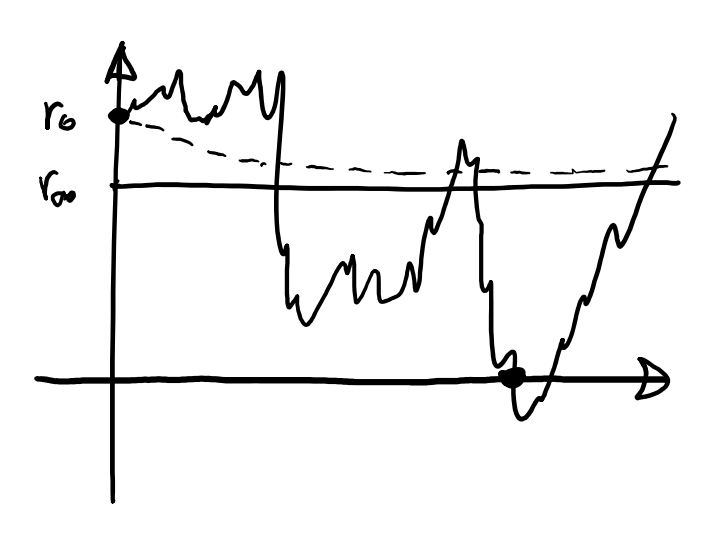
\includegraphics[scale=0.3]{fig/tmp/fig30.png}
        \captionof{figure}{Dynamics of the interest rate $r_t$ with initial condition $r_0$ and asymptotic value $r_{\infty}$.}
    \end{center}
    In order to find the solution of eq. \eqref{vasmodel}, we consider the following differential:
    \begin{align}
        \notag \dd(r_te^{bt}) &= e^{bt}\dd r_t + r_t\dd e^{bt} \\
        &=
        \notag e^{bt}(a-br_t)\dd t + e^{bt}\sigma_r \dd W^{\Qmeas} + br_te^{bt}\dd t \\
        &=
        ae^{bt}\dd t + \sigma_r e^{bt} \dd W^{\Qmeas}(t)
    \end{align}
    Integrating from 0 to $t$, we get:
    \begin{align}
        r_t e^{bt} - r_0 = \frac{a}{b}(e^{bt}-1) + \sigma_r \int_0^t e^{bs}\,\dd W^{\Qmeas}(s)
    \end{align}
    from which:
    \begin{equation}
        r_t = r_0e^{-bt} + \frac{a}{b}(1-e^{-bt}) + \sigma_r \int_0^t e^{-b(t-s)}\,\dd W^{\Qmeas}(s)
    \end{equation}
    It is very simple to check that $e^{-b(t-s)}\in\mathcal{H}$, so the integral is a martingale, in particular a gaussian variable $\mathcal{N}\left(0;\sigma_r^2\int_0^te^{-2b(t-1)}\,\dd s\right) = \mathcal{N}\left(0;\frac{\sigma^2_r}{2b}\left(1-e^{-2bt}\right)\right)$. The deterministic part results in a shift in the mean, so we end up with:
    \begin{equation}
        r_t \sim \mathcal{N}\left(r_0 + \frac{a}{b}(1-e^{-bt});\frac{\sigma^2_r}{2b}\left(1-e^{-2bt}\right)\right)
    \end{equation}
    It turns out that in the Vašíček model the interest rate is a gaussian variable. In particular, $\Qmeas(r_t<0)>0$. In the past this fact represented a problem, because the short interest rate was supposed to be strictly positive. This convention was dropped after the 2008 crisis.\\
    The simpler product to price in this framework is the zero-coupon bond. We would like to check if the volatility of the process $S(t)/B(t,T)$ is deterministic or not. In order to do that, we try to limit ourselves to the minimal needed information about $B(t,T)$. \\
    If we fix $s\ge t$ as starting point, we have:
    \begin{equation}
        r_s = r_te^{-b(s-t)} + \frac{a}{b}(1-e^{-b(s-t)}) + \sigma_r \int_t^s e^{-b(s-u)}\,\dd W^{\Qmeas}(u).
    \end{equation}
    The price of the zero-coupon bond is given by:
    \begin{align}\label{B}
        B(t,T) = \expect_t\left[e^{-\int_t^Tr_s\,\dd s}\right].
    \end{align}
    First, we compute the integral:
    \begin{align}
        \notag -\int_t^Tr_s\,\dd s &= -r_t\int_t^T e^{-b(s-t)}\,\dd s - \frac{a}{b}\int_t^T(1-e^{-b(s-t)})\,\dd s - \\
        &\qquad\qquad\qquad
        - \sigma_r\int_t^T \left(\int_t^s e^{-b(s-u)}\,\dd W^{\Qmeas}_u\right)\dd u.
    \end{align}
    The first two integrals are easy to compute, while the third is feasible thanks to the stochastic Fubini theorem. Since there is not dependence on the interest rate, the third integral will result in a Gaussian variable $\mathcal{N}(0;\Sigma^2)$ with zero mean and variance given by the Itô's isometry. If we solve the first integral and we consider the second integral as a shift in the mean, we end up with:
    \begin{align}
        -\int_t^Tr_s\,\dd s = -\dfrac{r_t}{b}(e^{-b(T-t)}-1) - \mathcal{N}(m;\Sigma^2)
    \end{align}
    Plugging in eq. \eqref{B} we get:
    \begin{equation}
        B(t,T) = \expect_t\left[e^{-\frac{r_t}{b}(e^{-b(T-t)}-1)}e^{-\mathcal{N}(m;\Sigma^2)}\right]
    \end{equation}
    By Itô, the dynamic of the zero-coupon bond is:
    \begin{align}
        \notag\dd B(t,T) &= \pdv{B(t,T)}{t}\,\dd t + \pdv{B(t,T)}{r_t}\,\dd r_t + \frac{1}{2}\pdv[2]{B(t,T)}{r_t}\,\dd\expval{r}_t \\
        \overset{\eqref{vasmodel}}&{=}
        \notag(\dots)\,\dd t + B(t,T)\frac{e^{-b(T-t)}-1}{b}((a-br_t)\dd t + \sigma_r\,\dd W^{\Qmeas}) \\
        \overset{(a)}&{=}
        (\dots)\,\dd t + B(t,T)\frac{e^{-b(T-t)}-1}{b}\sigma_r\,\dd W^{\Qmeas}
    \end{align}
    and then:
    \begin{align}\label{dbb}
        \frac{\dd B(t,T)}{B(t,T)} = (\dots)\,\dd t + \frac{e^{-b(T-t)}-1}{b}\sigma_r\,\dd W^{\Qmeas}
    \end{align}
    So, the volatility of $B(t,T)$ in the Vašíček model is given by:
    \begin{equation}
        \sigma_B = \frac{e^{-b(T-t)}-1}{b}
    \end{equation}
    Now, if we consider the ratio
    \begin{equation}
        \frac{\dd\frac{S(t)}{B(t,T)}}{\frac{S(t)}{B(t,T)}} = \hlc{mypink}{\left(\sigma-\sigma_r\frac{e^{-b(T-t)}-1}{b}\right)}\dd W^{\Qmeas} + (\dots)\,\dd t
    \end{equation}
    we have that the highlighted term is deterministic, so it is possible to find the B\&S formula for the price of a call in the Vašíček model. If we denote
    \begin{equation}
        \sigma-\sigma_r\frac{e^{-b(T-t)}-1}{b} \equiv \sigma_z
    \end{equation}
    then we have
    \begin{align}
        \call_t = S(t)\Phi(d_1)-KB(t,T)\Phi(d_2)
    \end{align}
    with
    \begin{align}
        d_1 = \dfrac{\ln\dfrac{S(t)}{B(t,T)K}-\frac{1}{2}\int_t^T\norm{\sigma_Z}^2\,\dd s}{\sqrt{\int_t^T\norm{\sigma_Z}^2\,\dd s}}
    \end{align} % d_1 o d_2?? prima questo era d_2
    Notice that, as expected, the zero-coupon bond becomes deterministic at the maturity (it gives one unit of money), in fact for $t=T$ eq. \eqref{dbb} becomes
    \begin{equation*}
        \frac{\dd B(t,T)}{B(t,T)} = (\dots)\,\dd t + \frac{e^{-b(T-T)}-1}{b}\sigma_r\,\dd W^{\Qmeas} = (\dots)\,\dd t.
    \end{equation*}
    In conclusion:
    \begin{itemize}
        \item in this particular model we are able to find the price for the zero-coupon bond (but we are not really interested in it), ending up with $B(t,T)$ having a log-normal distribution.
        \item We focused on the dependence of the stochastic quantity $r_t$, because in order to find out which is the dynamics of the zero-coupon bond we need the coefficient of the Brownian motion and according to Itô's formula this coefficient is only related to $\dd r_t$.
        \item We found the volatility of the zero-coupon bond and then we checked that the volatility of the process $S(t)/B(t,T)$ is deterministic. Then, if the volatility is deterministic, we can write down an explicit B\&S formula with CDFs $\Phi(d_1),\Phi(d_2)$. Is is surprising? No, because in general we know that:
        \begin{equation*}
            S(t) = S(0)\exp{\int_0^T r_s\,\dd s - \frac{1}{2}\sigma^2 t + \sigma\dd W^{\Qmeas}(t)}
        \end{equation*}
        In the Vašíček model $r_t$ is gaussian, so $\int_0^T r_s\,\dd s$ is gaussian too, together with $\dd W^{\Qmeas}(t)$. This means that $S(t)$ is log-normal distributed and that we can adopt the B\&S model.
    \end{itemize}
\end{example}

\section{Black formula}\lesson{18}{17/04/2020}
The B\&S formula gives the price of a call option on an asset. The purpose of this section is to derive the Black formula for the price of call options on a \emph{futures} or \emph{forward contract}.\\

\subsection{Forward contracts} % Hull ch.2
Recall the main features of the forward contract:
\begin{itemize}
    \item it gives us the obligation to buy the asset at a fixed price $K$ which is fixed at the signature date;
    \item the payoff is $(S_T-K)$;
    \item the strike $K$ is such that at the signature time the value of the contract is zero (it is cost-less to enter in a forward contract). Furthermore, we can introduce the notion of \emph{forward price} $K(t,T)$, which is the strike price decided at time $t$ such that the value of the ``new contract" starting at time $t$ is zero. In other words, it represents an ``updated baricenter";
    \item using the absence of arbitrage, we found that if the interest rate is constant then
    \begin{equation}
        K(0,T) = S(0)e^{r(T)} \qquad\Rightarrow\qquad K(t,T) = S(t)e^{r(T-t)}.
    \end{equation}
    If the interest rate is stochastic we have to consider a change of numéraire.
    \item if the strike $K(0,T)=K$ is the fair one, the price is given by:
    \begin{equation}\label{pr03}
        price_t(\pay_{[0,T]}) =
        \begin{cases}
        0 & t=0 \\
        \expect_t\left[e^{-\int_t^T r_s\,\dd s}(S(T)-K(0,T))\right] & 0<t<T \\
        S(T)-K(0,T) & t=T
        \end{cases}
    \end{equation}
    Let's compute the expected value in \eqref{pr03} for $0<t<T$:
    \begin{align*}
        \eqref{pr03} &= e^{-\int_t^T r_s\,\dd s}\expect_t\left[e^{-\int_0^T r_s\,\dd s}(S(T)\right] - K(0,T)B(t,T) \\
        \overset{(a)}&{=}
        \cancel{e^{-\int_0^t r_s\,\dd s}}\cancel{e^{-\int_0^t r_s\,\dd s}}S(t)- - K(0,T)B(t,T) \\
        &=
        S(t) - K(0,T)B(t,T)
    \end{align*}
    where in (a) we used the fact that the discounted asset $S(t)e^{-\int_0^t}r_s\,\dd s$ is a true $\Qmeas$-martingale. \\
    If the interest rate is flat, $r_t = r$ $\forall t$, we have:
    \begin{align}\label{eq4}
        price_t(S(T)-K(0,T)) = S(t) - K(0,T)e^{-r(T-t)} \gtrless 0
    \end{align}
    which can be positive or negative. Introducing the expression forward strike at time $t$:
    \begin{equation*}
        K(t,T) = S(t)e^{r(T-t)} \qquad\Rightarrow\qquad K(0,T) = S(0)e^{rT}
    \end{equation*}
    we can rewrite \eqref{eq4}:
    \begin{align}
        \label{eq1}
        price_t(S(T)-K(0,T)) &= S(t) - K(0,T)e^{-r(T-t)} \\
        &=
        \notag S(t) - S(0)e^{rT}e^{-r(T-t)} \\
        &=
        S(t) - S(0)e^{rt} \label{eq2}
    \end{align}
    Eq. \eqref{eq1} is a \emph{forward looking} expression, in the sense that we look for the correct price to exchange with the underlying at time $T$, we discount it and we compare this with the current realization of the underlying $S(t)$. Eq. \eqref{eq2} is a \emph{backward looking} expression, in the sense that the value of the forward contract is positive or negative according to the comparison between the current value of the underlying $S(t)$ and the capitalization of the initial value $S(0)$.
\end{itemize}

\subsection{Futures contracts}
Futures contracts are a particular type of forward contracts in which the counterparts ``do not know/trust each other". If the two counterparts agree to trade an asset in the future for a certain price, there are obvious risks. One of the investors may regret the deal and try to back out. Alternatively, the investor simply may not have the financial resources to honor the agreement. One of the key roles of the exchange is to organize trading so that contract defaults are avoided. This is where futures contracts and margin accounts come in.\\
Instead of signing the contract at time $t=0$ and hope that at time $T$ our counterpart will deliver the corresponding payoff (which can be positive or negative), we require it to deposit funds in a \emph{margin account}. The amount that must be deposited at the time the contract is entered into is known as the \emph{initial margin} and, at the end of each trading day, the margin account is adjusted to reflect the investor's gain or loss $S(t)\gtrless K$. This practice is referred to as \emph{daily settlement} or \emph{marking to market}.
\begin{figure}[ht]
    \centering
    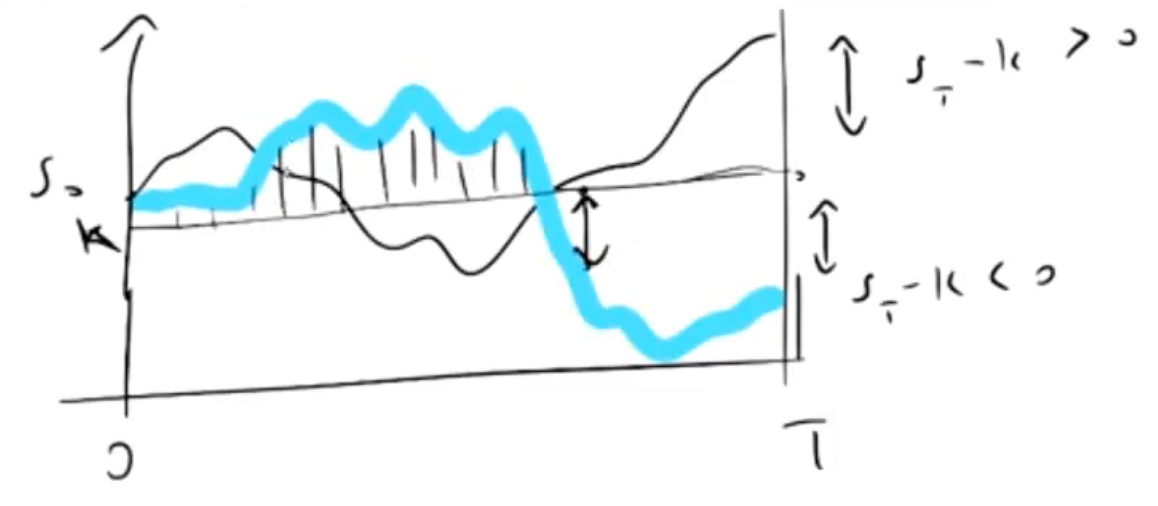
\includegraphics[scale=0.27]{fig/tmp/fig31.png}
    \caption{Futures contracts.}
    \label{fig:futures}
\end{figure}
\newline The investor is entitled to withdraw any balance in the margin account in excess of the initial margin. To ensure that the balance in the margin account never becomes negative a \emph{maintenance margin}, which is somewhat lower than the initial margin, is set. If the balance in the margin account falls below the maintenance margin, the investor receives a \emph{margin call} and is expected to top up the margin account to the initial margin level by the end of the next day. The extra funds deposited are known as \emph{variation margin}. If the investor does not provide the variation margin, the broker closes out the position\footnote{See \cite{hull}, section 2.4.}.\\
\\
Here we will consider a simplified marking to market framework in which we make the following assumptions:
\begin{itemize}
    \item the market to market is on the whole value of the contract, in such a way that if the payoff of the futures at time $T$ is $S(T)-F(0,T)$, then:
    \begin{equation*}
        price_t(\fut) \equiv 0 \quad\forall t
    \end{equation*} % fine parte 1
    \item for all $t$ there is a quoted strike price $F(t,T)$ called \emph{strike price} which makes zero the value of the contract. This means that in the time interval $(s,t]$ the holder of a futures receives the dividend $F(t,T) - F(s,T)$.\\
    For example, if there is a shock in the market so that $F(t,T) - F(s,T) < 0$, the long position has to pay this difference (margin call).
    \item The convergence condition
    \begin{equation}
        F(T,T) = S(T)
    \end{equation}
    holds.
    \begin{figure}[h]
        \centering
        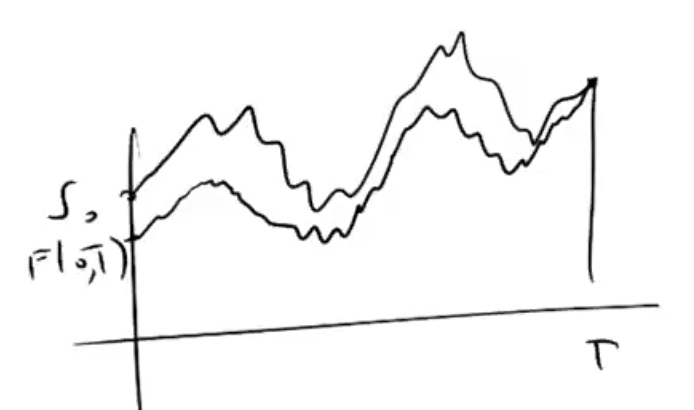
\includegraphics[scale=0.32]{fig/tmp/fig32.png}
        \caption{Converge condition of the underlying}
        \label{fig:concond}
    \end{figure}
\end{itemize}
In summary:
\begin{itemize}
    \item $price_t = 0$ $\forall t\le T$ (this plays the role of $S_t$);
    \item The dividend is equal to the futures price: $D(t)=F(t,T)$;
    \item $F(T,T)=S(T)$ (boundary condition).
\end{itemize}
From Section \ref{B&Swithdividends} we know that in presence of dividends the discounted asset is not a martingale, but the normalized gain process
\begin{align}
    S(t)e^{-\int_0^t r_s\,\dd s} + \int_0^t e^{-\int_0^s r_u\,\dd u}\dd D
\end{align}
is a $\Qmeas$-martingale. But in futures contracts
\begin{equation*}
    S(t) \leftrightarrow price_t \equiv 0, \quad \dd D = \dd F
\end{equation*}
so we are left with:
\begin{align}\label{it}
    \int_0^t e^{-\int_0^s r_u\,\dd u}\,\dd F_s \overset{(a)}{=} \int_0^t h_s\,\dd W_s^{\Qmeas}
\end{align}
where in (a) we used the representation theorem of continuous (Brownian) martingales, which allows us to write the integral as a Brownian integral introducing an appropriate adapted process $h_s$. Writing \eqref{it} in its infinitesimal form we have:
\begin{equation}
    e^{-\int_0^s r_u\,\dd u}\,\dd F_t = h_s\,\dd W_s^{\Qmeas} \qquad\Rightarrow\qquad \dd F(t,T) = \left(e^{\int_0^s r_u\,\dd u}h_t\right)\,\dd W_s^{\Qmeas}.
\end{equation}
In other words, we have that $F(t,T)$ is a $\Qmeas$-martingale. So, by martingality, the futures' price at time $t$ is given by:
\begin{equation}
    F(t,T) = \expect_t[F(T,T)] = \expect_t[S(T)] = \expect[S(T)|\mathcal{F}_t]
\end{equation}
Recall that for the forward contract we found that:
\begin{equation}
    K(t,T) = \expect_t\left[\dfrac{e^{-\int_t^T r_s\,\dd s}S(T)}{B(t,T)}\right] = \mathbb{E}^{\Qmeas^T}_t[S(T)]
\end{equation}
So forward price and futures price are both the expected value of the underlying at time $T$ but they are computed under different probability measures (forward risk neutral measure and risk neutral measure). \\
Forward price and futures are the same if the two probability measures are the same. For example, this is true when the interest rate is deterministic.

\subsection{Black formula} % Bjork pag. 108
The Black formula gives the price of a call on a futures (on $S$). Here we assume that the underlying evolves according to the B\&S dynamics with constant interest rate, $r_t \equiv r$. In this framework, if we denote with $X$ the strike price of the call and we choose $T_1 > T$ as maturity of the call option, the payoff is
\begin{equation}
    \pay_T = (F(T,T_1) - X)^+ + \underbrace{\pay_T(\text{long position on the futures})}_{=0}
\end{equation}
In other words, we have a contract on a contract, which is called \emph{compounded option}. \\
Using eq. \eqref{eq2} we can write:
\begin{align}
    \notag (F(T,T_1) - X)^+ &= \left(S(T)e^{r(T_1-T)} - X\right)^+ \\
    &=
    e^{r(T_1-T)}\left(S(T)-Xe^{-r(T_1-T)}\right)^+
\end{align}
Recall that according to the B\&S formula the price of a call is given by:
\begin{equation*}
    price_t(\call) = S(t)\Phi(d_1)-Ke^{-r(T-t)}\Phi(d_2)
\end{equation*}
In this case
\begin{equation*}
    K = Xe^{-r(T_1-T)}, \qquad S(t) = F(t,T_1)e^{-r(T_1-t)}
\end{equation*}
so we have:
\begin{align*}
    price_t(\call(\fut)) &= e^{-r(T_1-T)} \left(S(t)\Phi(d_1)-e^{-r(T-t)}Xe^{-r(T_1-T)}\Phi(d_2)\right) \\
    &=
    e^{-r(T_1-T)}S(t)\Phi(d_1)-e^{-r(T-t)}Xe\Phi(d_2) \\
    &=
    e^{-r(T-t)}\left(\underbrace{S(t)e^{-r(T_1-t)}}_{F(t,T_1)}\Phi(d_1) - X\Phi(d_2)\right)
\end{align*}
We end up with the so called \emph{Black formula}:
\begin{equation}
    price_t(\call(\fut)) = e^{-r(T-t)}\left(F(t,T_1)\Phi(d_1) - X\Phi(d_2)\right)
\end{equation}
where in this case:
\begin{equation}
    d_1 = \dfrac{\ln\frac{F(t,T_1)}{X}+\frac{1}{2}\sigma^2(T-t)}{\sigma\sqrt{T-t}}, \qquad d_2 = d_1 - \sigma\sqrt{T-t}. %giusto
\end{equation}

\section{Quantity-adjusted options}\lesson{19}{22/04/2020} % Bjork pag. 248
Quantity-adjusted options, also called \emph{quanto} options, are cash settled, cross currency derivatives where the underlying asset is denominated in a currency different from the one in which the option is settled. In other words, quanto options are derivatives where the payoff is defined by variables associated with one currency but is paid in another currency. \\
For example, the transfer between \EUR{1} and 1\,\$ is given through an \emph{exchange rate}
\begin{equation}
    X(t)^{\text{EURUSD}} = \dfrac{\text{\EUR{1}}}{1\,\$}
\end{equation}
which is usually given using the \emph{FORDOM} (foreign-domestic currency) notation. If we consider a third additional currency, for example the Japanese Yen \textyen, in order to be consistent it must be that if $X_1, X_2$ are two exchange rates, then $X_3 = X_1X_2$. So, the product of two exchange rates is an exchange rate.\\
In general, the interest rates in different countries are different, so  -- at least in principle -- there can be a potential arbitrage opportunity. However, this is only an apparent problem since, as soon as we may want to exploit this arbitrage, we would have to consider the currency conversion, which works through a stochastic quantity, the interest rate. \\
As starting point, we assume that the evolution of the exchange rate between the two currencies is given by a B\&S dynamics under the subjective probability measure $\Pmeas$:
\begin{align}
    \frac{\dd X(t)}{X(t)} = \mu_X\,\dd t + \sigma_X\,\dd W^{\Pmeas}(t)
\end{align}
This is a good candidate, in fact the products of two Brownian motions is itself a Brownian motion. The evolution of the corresponding riskless asset in the domestic currency is given by:
\begin{align}\label{dd}
    \frac{\dd B_d}{B_d} = r_d\,\dd t
\end{align}
Similarly, the riskless asset in the foreign currency evolves according to the equation:
\begin{equation}\label{fffffffffffff}
    \frac{\dd B_f}{B_f} = r_f\,\dd t
\end{equation}
We already know the solutions of \eqref{dd} and \eqref{fffffffffffff}:
\begin{equation}
    B_d(t) = e^{r_d t}, \qquad B_f(t) = e^{r_f t}
\end{equation}
Here we assume that $r_d, r_f$ are constant and that if we buy foreign currency, this will evolve according $r_f$\footnote{This is not always the case. For example, if we buy dollars in the euro-zone the evolution of this EUR-dollar is different from the one of USD-dollar. Anyway, this is a reasonable assumption.}. \\
We want to price options on the exchange rate at maturity $X_T$. Notice that these are not properly quanto options, because we need to introduce an underlying denominated in a different currency. For example, consider the call option that allows to buy 1\,\$ at price \EUR{$K$}, which has payoff $(X_T-K)^+$. According to the risk neutral methodology the price is given by:
\begin{align*}
    price_t = e^{-r(T-t)}\expect_t[(X_T-K)^+]
\end{align*}
But we are not able to define the risk neutral measure $\Qmeas$ if there is no underlying. In fact, in order to find $\Qmeas^d$ we have to impose that whatever discounted asset in our country is a martingale, i.e. it evolves with a drift $r_d$. \\
Which are the domestic assets? Let's consider a stylized economy in which we have the foreign and domestic saving accounts and we consider the transfers between the two. In this case there are two assets:
\begin{itemize}
    \item $B_d$, in fact its drift is $r_d$;
    \item $B_fX = \Tilde{B}_f$, i.e. the foreign riskless asset converted into the domestic currency.
\end{itemize}
By Itô, we have that:
\begin{align}\label{al1}
    \notag\dd\Tilde{B}_f &= \dd(B_fX) = (\dd B_f)X + B_f\,\dd X \\
    &=
    \notag\Tilde{B}_f r_f\, \dd t + \Tilde{B}_f(\mu_X\,\dd t + \sigma_X\,\dd W^{\Pmeas}) \\
    &=
    \Tilde{B}_f(\mu_X + r_f)\,\dd t + \Tilde{B}_f\sigma_X\,\dd W^{\Pmeas}
\end{align}
This is the general dynamics of a foreign riskless asset converted in the domestic currency. Now we want that
\begin{equation*}
    \mu_X + r_f = r_d
\end{equation*}
so we perform the same trick we used when we applied the martingale approach to the B\&S model, that is we absorb the excessive drift into the Brownian motion:
\begin{equation}\label{al2}
    \eqref{al1} = \Tilde{B}_f\left(r_d\,\dd t + \sigma_X\left(\dd W^{\Pmeas} + \dfrac{\mu_X + r_f-r_d}{\sigma_X}\,\dd t\right)\right)
\end{equation}
If we define the change of probability measure given by the Radon-Nikodym derivative\footnote{$\mathcal{E}$ is the so called \href{https://en.wikipedia.org/wiki/Dol\%C3\%A9ans-Dade\_exponential}{Doléans-Dade exponential}.}:
\begin{align}
    \notag\eval{\frac{\dd \Qmeas^d}{\dd \Pmeas}}_t &= \mathcal{E}\left(\dfrac{\mu_X + r_f-r_d}{\sigma_X}\right)_t \\
    &=
    \notag\exp{\int_0^t \left(\dfrac{\mu_X + r_f-r_d}{\sigma_X}\right)\,\dd W^{\Pmeas} - \int_0^t \left(\dfrac{\mu_X + r_f-r_d}{\sigma_X}\right)^2\,\dd s} \\
    &\sim
    \exp{\alpha W(t) - \frac{1}{2}\sigma^2 t} = \text{true martingale}
\end{align}
we can apply the Girsanov theorem:
\begin{equation*}
    \dd W^{\Pmeas} + \dfrac{\mu_X + r_f-r_d}{\sigma_X}\,\dd t = \dd W^{\Qmeas^d}
\end{equation*}
Then:
\begin{align}
    \dd\Tilde{B}_f &= \Tilde{B}_f(r_d\,\dd t + \sigma_X\dd W^{\Qmeas^d})
\end{align}
So, the dynamics of $X_t$ under the domestic risk neutral pricing probability measure $\Qmeas^d$ is given by:
\begin{equation}\label{dynX}
    \dfrac{\dd X_t}{X} = (r_d - r_f)\dd t + \sigma_X\,\dd W^{\Qmeas^d}
\end{equation}
In a sense, the short foreign interest rate $r_f$ plays the role of a dividend.
\begin{remark}
    Notice that the exchange rate $X/B^d$, i.e. the discounted $X$, is not a $\Qmeas^d$-martingale. This is confirmed by the fact that there is an additional drift $r_f$.
\end{remark} % fine prima parte
Now we are ready to price an exchange option.
\begin{proposition}
    The price at time $t$ of whatever payoff written on the exchange rate at maturity $T$ is given by:
    \begin{itemize}
    \item the discounted value under the domestic interest rate of the conditional risk neutral expectation of the payoff:
    \begin{equation}
    price_t = e^{-r_d(T-t)}\mathbb{E}^{\Qmeas^d}_{t,X}[\pay(X_T)]
    \end{equation}
    where the dynamics of $X_t$ is given by \eqref{dynX};
    \item the solution:
    \begin{equation}
        price_t = F(t,X_t)
    \end{equation}
    of the PDE:
    \begin{equation}
        \begin{cases}
        \pdv{F}{t} + (r_d-r_f)X\pdv{F}{X} + \frac{1}{2}X^2\sigma_X^2\pdv[2]{F}{X} - r_dF = 0\\
        F(X,T) = \pay(X)
        \end{cases}
    \end{equation}
    \item the solution \begin{equation}
        F(t,X) = F_0(t,Xe^{-r_f(T-t)})
    \end{equation}
    where $F_0$ is the solution corresponding to no dividends, which obeys to the equation:
    \begin{equation}
        \frac{\dd X}{X} = r_d\dd t + \sigma_X\dd W^{\Qmeas}
    \end{equation}
    \end{itemize}
\end{proposition}
\begin{example}{Call option on the exchange rate}{}{}
    The price of a call option on $X$ is given by:
   \begin{align}
       price_t(\call\text{ on } X) = X_t e^{-r_f(T-t)}\Phi(d_1) - e^{-r_d(T-t)}K\Phi(d_2)
   \end{align}
   where
   \begin{equation}
       d_1 = \frac{1}{\sigma_X\sqrt{T-t}}\left(\ln\frac{X_te^{-r_f(T-t)}}{K}+\left(r_d+\frac{1}{2}\sigma_X^2\right)(T-t)\right)
   \end{equation}
   \begin{equation}
       d_2 = \frac{1}{\sigma_X\sqrt{T-t}}\left(\ln\frac{X_te^{-r_f(T-t)}}{K}+\left(r_d-\frac{1}{2}\sigma_X^2\right)(T-t)\right)
   \end{equation}
\end{example}
Yet, we are not ready to price quanto options. We need to do an upgrade, introducing in the market some risky assets. The starting point is that the dynamics under $\Pmeas$ is given by
\begin{equation}
    \frac{\dd X}{X} = \mu_X\,\dd t + \sigma_X\cdot\dd W^{\Pmeas}
\end{equation}
for the exchange rate, by
\begin{equation}\label{Sd}
    \frac{\dd S_d}{S_d} = \mu_d\,\dd t + \sigma_d\cdot\dd W^{\Pmeas}
\end{equation}\label{Sf}
for the domestic asset and by
\begin{equation}
    \frac{\dd S_f}{S_f} = \mu_f\,\dd t + \sigma_f\cdot\dd W^{\Pmeas}
\end{equation}
for the foreign asset. We used the scalar product $(\cdot)$ because $\sigma$ is a row vector and $\dd W$ is a column vector.\\
The volatility matrix of our market is given by
\begin{equation}
    \sigma =
    \begin{pmatrix}
    \sigma_X \\ \sigma_d \\ \sigma_f
    \end{pmatrix} =
    \begin{pmatrix}
    \sigma_{X_1} & \sigma_{X_2} & \sigma_{X_3} \\
    \sigma_{d_1} & \sigma_{d_2} & \sigma_{d_3} \\
    \sigma_{f_1} & \sigma_{f_2} & \sigma_{f_3}
    \end{pmatrix}
\end{equation}
We also add a domestic and a foreign riskless assets which evolve according to the equations:
\begin{align}
    \frac{\dd B_d}{B_d} &= r_d\,\dd t \\
    \frac{\dd B_f}{B_f} &= r_f\,\dd t
\end{align}
Now we can consider different problems involving different contract. For example:
\begin{itemize}
    \item pricing in euros a call on $S_f$ in dollars with $K$ in dollars, which has payoff $(S_f(T)-K)^+X_T^{\text{USDEUR}}$ (not a real quanto option);
    \item pricing in euros a call on $S_f$ in dollars with $K$ in euros, which has payoff $(S_fX_T-K)^+$ (real quanto option).
\end{itemize}
Now we have to characterize the probability measure $\Qmeas^d$ under which we price this payoffs. Again, we impose that under $\Qmeas^d$ all the domestic assets discounted by the domestic interest rate are $\Qmeas^d$-martingales, i.e. the domestic assets evolve with drift $r_d$. Our domestic assets are $B_d, S_d, \Tilde{S}_f = S_fX_t$ and $\Tilde{B}_f = B_fX_t$, so this quantities have -- once discounted by $B_d$ -- must be $\Qmeas^d$-martingales.\\
Let's start from $S_d$ and rewrite \eqref{Sd} in such a way that the drift is $r_d$:
\begin{align}
    \frac{\dd S_d}{S_d} = r_d\,\dd t + \sigma_d\left(\dd W^{\Pmeas} + \frac{\mu_d-r_d}{``\sigma_d"}\,\dd t\right)
\end{align}
This is only a formal expression because, since $\sigma_d$ is a row vector, $\nicefrac{1}{\sigma_d}$ is not well defined.\\
Then we have:
\begin{align}
    \notag\frac{\dd\Tilde{S}_f}{\Tilde{S}_f} &= (\mu_f+\mu_X+\sigma_f\sigma^T_X)\,\dd t + (\sigma_f + \sigma_d)\dd W^{\Pmeas} \\
    &=
    r_d\,\dd t + (\sigma_f+\sigma_X)\left(\dd W^{\Pmeas}+\dfrac{\mu_f + \mu_X + \sigma_f\sigma_X^T - r_d}{``\sigma_f\sigma_X"}\,\dd t\right)
\end{align}
which again is just a formal expression. Finally, we can do the same thing for the foreign riskless asset denominated in the domestic currency:
\begin{align}
    \notag\frac{\dd\Tilde{B}_f}{\Tilde{B}_f} &= (\mu_f+\mu_X)\,\dd t + \sigma_X\dd W^{\Pmeas} \\
    &=
    r_d\,\dd t + \sigma_X\left(\dd W^{\Pmeas}+\dfrac{\mu_X + r_f - r_d}{``\sigma_X"}\,\dd t\right)
\end{align}
Provided that the Girsanov Theorem can be applied to a 3-dimensional geometric Brownian motion $W^{\Pmeas}$ we have to find the corresponding Radon-Nikodym derivative
\begin{equation} % 24:00
    \eval{\dfrac{\dd\Qmeas^d}{\dd\Pmeas}}_t = \colorbox{cyan}{homework}
\end{equation}
Now, for example, consider the problem of pricing in euros a call on $S_f$ in dollars with $K$ in dollars, which has payoff $(S_f(T)-K)^+X_T^{\text{USDEUR}}$. We can solve this problem by pricing directly in the foreign country, that is under $\Qmeas^f$, using the B\&S model and then convert the result using the exchange rate:
\begin{equation}
    price = X_t(S_f(t)\Phi(d_1)-e^{-r_f(T-t)}K\Phi(d_2))
\end{equation}
where
\begin{equation}
    d_1 = \frac{1}{\norm{\sigma_f}\sqrt{T-t}}\left(\ln\frac{S_f(t)}{K}+\left(r_f+\frac{1}{2}\norm{\sigma_f}^2\right)(T-t)\right)
\end{equation}
Again, we see that this is not a real quanto problem but just a matter of conversion.
Let's consider the real quanto option problem, i.e. pricing in euros a call on $S_f$ in dollars with $K$ in euros, which has payoff $(S_f X_T-K)^+$. This is a call written on $\Tilde{S}_f$ so we can apply the $\Qmeas^d$-pricing methodology on it. So, the price of this quanto option is:
\begin{equation}
    price_t((S_f X_T-K)^+) = \Tilde{S}_f(t)\Phi(d_1)-e^{-r_d(T-t)}K\Phi(d_2)
\end{equation}
with
\begin{equation}
    d_1 = \frac{1}{\norm{\sigma_X+\sigma_f}\sqrt{T-t}}\left(\ln\frac{\Tilde{S}_f(t)}{K}+\left(r_d+\frac{1}{2}\norm{\sigma_X+\sigma_f}^2\right)(T-t)\right)
\end{equation}
\begin{remark}
    $\Qmeas^d \ne \Qmeas^f$ (Siegel paradox). This happens because under $\Qmeas^d$ we impose that everything in the domestic market -- after being discounted by the domestic interest rate -- is a martingale while under $\Qmeas^f$ we impose that all the foreign assets, including the domestic ones converted in the foreign currency, will be martingales -- once discounted by the foreign riskless asset. This leads to different dynamics. In particular, the exchange rate under $\Qmeas^d$ evolves according to the equation:
    \begin{equation}
       \frac{\dd X}{X} = (r_d-r_f)\,\dd t + \sigma_X\,\dd W^{\Qmeas^d}
    \end{equation}
    Consider the euro-zone and the dollar-zone. If the exchange rate between euros and dollars is $X$ then the one from dollars to euros must be $\nicefrac{1}{X}$. But the dynamics under $\nicefrac{1}{X}$ is given by
    \begin{equation}
        \frac{\dd\frac{1}{X}}{\frac{1}{X}} = (r_d-r_f\hlc{mypink}{\norm{\sigma_X}^2})\,\dd t + \sigma_X\,\dd W^{\Qmeas^d}
    \end{equation}
    so there is an additional term, essentially the Itô term, which is responsible for the fact that the two measures are not the same. This is due to the randomness of the exchange rate.
\end{remark}
\begin{example}{Quanto exchange call}{}{}
    Price the exchange quanto option, which has payoff:
    \begin{equation*}
        (X_TS_f(T)-S_d(T))^+ = (\Tilde{S}_f(T)-S_d(T))^+
    \end{equation*}
    \colorbox{cyan}{Homework}.
\end{example}

\section{Barrier options}\lesson{20}{23/04/2020} 
A \emph{barrier option} is a type of derivative where the payoff depends on whether or not the underlying asset has reached or exceeded a predetermined price. In order to deal with the past history of the underlying we need some stochastic analysis tools. 

\subsection{Mathematical background} 
\begin{definition}[Mirror reflection]
The \emph{mirror reflection of a Brownian motion} $B(t)$ at the level $m$ and in the interval $[\tau,T]$ is defined as:
    \begin{equation}
        \Tilde{B}(t) = \begin{cases}
            B(t) & t<\tau \\
            2m - B(t) & \tau \le t\ge T
        \end{cases}
    \end{equation}
\end{definition}
The idea is that if we have an object in a point $b$ and if in a point $m<b$ we put a mirror, then the image of $b$ with respect to $m$ will be at $2m-b$.  
\begin{figure}[h]
    \centering
    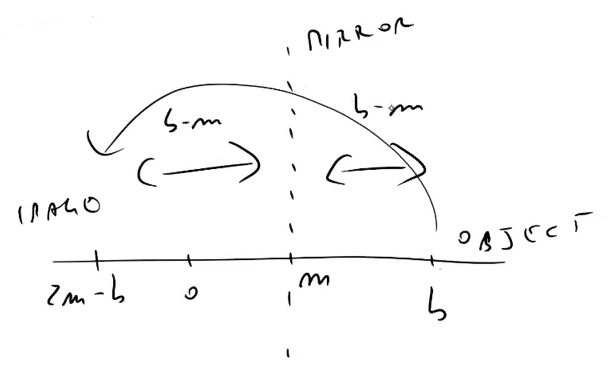
\includegraphics[scale=0.3]{fig/tmp/fig33.png}
    \caption{Mirror reflection.}
    \label{fig:mirro}
\end{figure}
\newline One fundamental property is that, if the Brownian motion crosses the barrier at $m$, then
\begin{equation}
    \Pmeas(B(T)>x) = \Pmeas(\Tilde{B}(T)>2m-x)
\end{equation}
In order to have an intuition about that, look at Figure \ref{fig:bmmirror}. For $t>\tau$ we can consider the original Brownian motion or its mirror reflection, so at time $T$ the probability that $B(T)>x$ is equal to the probability that $\Tilde{B}(T)<2m-x$.
\begin{figure}[h]
    \centering
    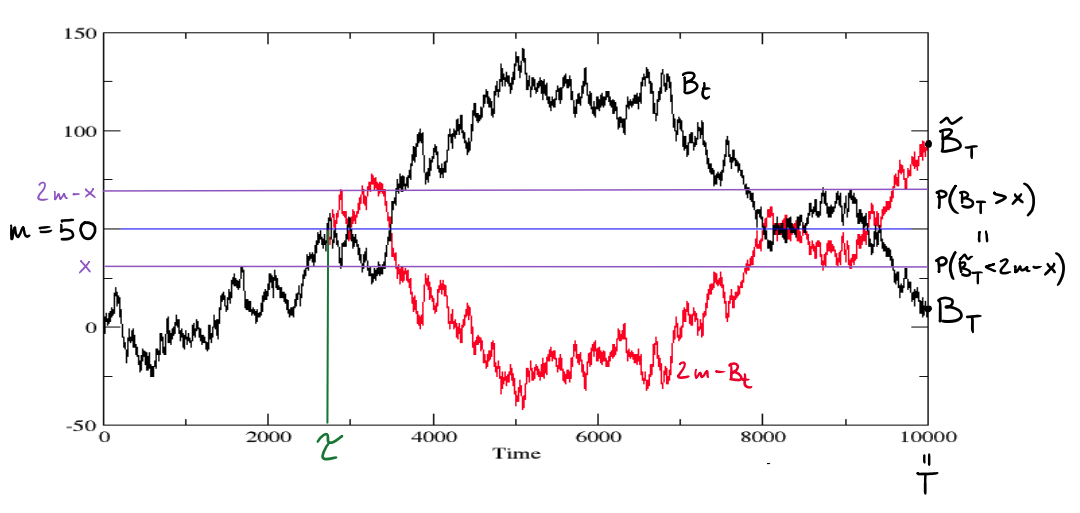
\includegraphics[scale=0.22]{fig/tmp/fig34.png}
    \caption{For $t>\tau$ we can consider the original Brownian motion or its mirror reflection.}
    \label{fig:bmmirror}
\end{figure}
\begin{definition}
    The the \emph{running maximum} of the Brownian motion $B(t)$ is defined as
    \begin{equation}
        M(t) = \sup_{0\le s\le t} B(s)
    \end{equation}
\end{definition}
\begin{definition}
    The \emph{first hitting time} is defined as
    \begin{equation}
        T_a = \inf\{t:B(t)=a\}, \qquad a>0 
    \end{equation}
\end{definition}
Since
\begin{equation*}
    \limsup_t B(t) = +\infty,
\end{equation*}
we have that 
\begin{equation}
    \Pmeas(T_a<\infty) = 1
\end{equation}
so the hitting time is finite but not bounded. \\
Another important property that comes from the definition of BM is that the increment $B(t+T)-B(T)$ is still a BM and it is independent of the filtration $\mathcal{F}_T$. This property holds also for stochastic times, for example the first hitting time:
\begin{equation}
    B(t+T_a) - B(T_a) = \text{Brownian motion } \indep\, \mathcal{F}_{s}\quad\forall s\le T_a
\end{equation}
Provided that the Brownian motion will reach $a$ at some time, we have that 
\begin{equation}\label{baa}
    B(T_a) = a,    
\end{equation}
so the Brownian motion at the random time $T_a$ becomes a (deterministic) constant.
\begin{theorem}[Reflection principle]
    Let $B(t)$ be a standard Brownian motion and let $a>0$. Then
    \begin{equation}
        \Pmeas(M(t) \ge a) = 2\Pmeas(B(t)\ge a) = \frac{2}{\sqrt{2\pi t}}\int_a^{+\infty}e^{-\frac{x^2}{2t}}\,\dd x.
    \end{equation}
\end{theorem}
\begin{proof}
    \begin{align*}
        \Pmeas(B(t)\ge a) &= \Pmeas(B(t)\ge a, M(t) \ge a) + \underbrace{\Pmeas(B(t)\ge a, M(t) < a)}_{=0} \\
        &=
        \Pmeas(B(t)\ge a | M(t) \ge a)\Pmeas(M(t) \ge a) \\
        \overset{\eqref{baa}}&{=}
        \hlc{mypink}{\Pmeas(B(T_a + (t-T_a)) - B(T_a) \ge 0 | M(t) \ge a)}\Pmeas(M(t) \ge a) \\
        &=
        \frac{1}{2}\Pmeas(M(t) \ge a)
    \end{align*}
    where we used the fact that the highlighted term is the probability of a Brownian motion, i.e. a Gaussian variable, to be greater than zero, i.e. $\nicefrac{1}{2}$.
\end{proof}
The importance of the reflection principle comes from the fact that it translates the problem of computing a $\Pmeas(M_t\ge a)$, which involves the whole past of the BM, in terms of the probability of a Brownian random variable, which is very simple, being Gaussian.\\
Now we need the probability of the joint distribution of the maximum of the BM and the BM itself.
\begin{proposition}
    For $a>0$ and $y\ge0$:
    \begin{equation}
        \Pmeas(M(t)\ge a, B(t)\le a-y) = \Pmeas(B(t)>a+y)
    \end{equation}
    Alternatively,
    \begin{equation}
        \Pmeas(M(t) > m, B(t)<b) = \Pmeas(B(t)>2m-b).
    \end{equation}
\end{proposition}
\begin{proof}
    \begin{align*}
        \Pmeas(B(t)>a+y) &= \Pmeas(B(t)>a+y, M(t)\ge a) + \underbrace{\Pmeas(B(t)>a+y, M(t)<a)}_{=0} \\
        \overset{(a)}&{=}
        \Pmeas(B(T_a+(t-T_a)) - a > -y|M(t)\ge a)\Pmeas(M(t)\ge a) \\
        &=
        \Pmeas(B(T_a+(t-T_a)) < a - y , M(t)\ge a) 
    \end{align*}
    where in (a) we used the symmetry of the BM.
\end{proof}
\begin{corollary}
    For any $a>0$ and $y\ge 0$
    \begin{equation}
        \Pmeas(M(t)\le a, B(t)\le a-y) = \Phi\left(\frac{a-y}{\sqrt{t}}\right)-\Phi\left(\frac{-a-y}{\sqrt{t}}\right).
    \end{equation}
\end{corollary}
\begin{proof}
    From the fact that 
    \begin{equation*}
        \Pmeas(B(t)<x) = \Pmeas(B(t)<x, M(t)<y) + \Pmeas(B(t)<x, M(t)\ge y) 
    \end{equation*}
    we have that 
    \begin{equation*}
        \Pmeas(M(t)\le a, B(t)\le a-y) = \Pmeas(B(t)\le a-y) - \Pmeas(B(t)\le a-y, M(t)>a)
    \end{equation*}
\end{proof}
By construction, the \emph{joint probability density} is given by
\begin{align}
    \notag\Pmeas(M(t)\in\dd m, B(t)\in\dd b) &= -\pdv{}{m}{b}\Pmeas(B(t)>2m-b) \\
    &=
    \frac{2(2m-b)}{\sqrt{2\pi t^3}}e^{\frac{(2m-b)^2}{2t}}\mathds{1}_{m\ge0}\mathds{1}_{m\ge b},
\end{align}
as we can see by computing
\begin{align*}
    -\pdv{}{m}{b}\dfrac{1}{\sqrt{2\pi t}}\int^{+\infty}_{2m-b}e^{-\frac{x^2}{2t}}\,\dd x 
    &= -\pdv{}{m}\left(\frac{1}{\sqrt{2\pi t}}e^{-\frac{(2m-b)^2}{2t}}\right) \\
    &=
    \dfrac{2(2m-b)}{\sqrt{2\pi t^3}}e^{-\frac{(2m-b)^2}{2t}}.
\end{align*}
From the reflection principle we have that
\begin{align}
    \notag\Pmeas(T_a\le t) &= \Pmeas(M(t)\ge a) = 2\Pmeas(B(t)\ge a) \\
    &= 
    \notag\dfrac{2}{\sqrt{2\pi t}}\int^{+\infty}_{a}e^{-\frac{x^2}{2t}}\,\dd x \\
    &=
    2\left(1-\Phi\left(\frac{a}{\sqrt{t}}\right)\right).
\end{align}
So, the density of the hitting time is given by
\begin{align}\label{hittimedens}
    \notag f_{T_a}(t) &= \pdv{\Pmeas(T_a \le t)}{t} \\
    &= 
    \notag -\frac{t^{-3/2}}{2}\frac{2}{\sqrt{2\pi}}\int^{+\infty}_{a}e^{-\frac{x^2}{2t}}\,\dd x + \frac{2}{\sqrt{2\pi t}} + \frac{2}{\sqrt{2\pi t}}\int^{+\infty}_{a}\frac{x^2}{2t^2} e^{-\frac{x^2}{2t}}\,\dd x \\
    \overset{(a)}&{=}
    \notag \cancel{-\frac{t^{-3/2}}{2}\frac{2}{\sqrt{2\pi}}\int^{+\infty}_{a}e^{-\frac{x^2}{2t}}\,\dd x} + \frac{2}{\sqrt{2\pi t}} + \frac{a}{\sqrt{2\pi t^3}}e^{-\frac{a^2}{2t}} + \cancel{\frac{1}{\sqrt{2\pi t^3}}\int_a^{+\infty} e^{-\frac{x^2}{2t}} \,\dd x} \\
    &=
    \frac{a}{\sqrt{2\pi t^3}}e^{-\frac{a^2}{2t}}\mathds{1}_{t>0}
\end{align}
where in (a) we computed the last integral:
\begin{align*}
    \frac{2}{\sqrt{2\pi t}}\int^{+\infty}_{a}\frac{x^2}{2t^2} e^{-\frac{x^2}{2t}}\,\dd x &= \frac{2}{\sqrt{2\pi t}}\int^{+\infty}_{a}\left(-\frac{x}{t}\right) e^{-\frac{x^2}{2t}}\left(-\frac{x}{2t}\right)\,\dd x \\
    &=
    \frac{2}{\sqrt{2\pi t}}\left(\eval{e^{-\frac{x^2}{2t}}\left(-\frac{x}{2t}\right)}_a^{+\infty} - \int_a^{+\infty}e^{-\frac{x^2}{2t}}\left(-\frac{1}{2t}\right)\,\dd x\right) \\
    &=
    \frac{a}{\sqrt{2\pi t^3}}e^{-\frac{a^2}{2t}} + \frac{1}{\sqrt{2\pi t^3}}\int_a^{+\infty} e^{-\frac{x^2}{2t}} \,\dd x.
\end{align*}
Now we can compute the moment generating function of $T_a$:
\begin{align}\label{momgen}
    \mathbb{E}[e^{\lambda T_a}] = \int_0^{\infty} e^{-\lambda t}\frac{a}{\sqrt{2\pi t^3}} e^{-\frac{a}{2t}}\,\dd t = \colorbox{cyan}{homework} = e^{-\sqrt{2\lambda} a}
\end{align}
where $\lambda>0$. An alternative way of computing it comes from the fact that $e^{\alpha B(t)-\frac{1}{2}\alpha^2 B(t)}$ is an exponential martingale, so
\begin{equation*}
    \mathbb{E}\left[e^{\alpha B(t)-\frac{1}{2}\alpha^2 t}\right] = 1
\end{equation*}
For the case in which $t=T_a$ we get:
\begin{align*}
    1 &= \mathbb{E}\left[e^{\alpha B(T_a)-\frac{1}{2}\alpha^2 T_a}\right] \overset{(a)}{=} 
    \xcancel{\mathbb{E}\left[e^{\alpha B(T_a)-\frac{1}{2}\alpha^2 T_a}\right]} \\
    &=
    \xcancel{\mathbb{E}\left[e^{\alpha a - \frac{1}{2}\alpha^2 T_a}\right] =
    e^{\alpha a}\mathbb{E}\left[e^{-\frac{1}{2}\alpha^2 T_a}\right]}
\end{align*}
However, in principle, the equality (a) is not true. In fact, in general, if $X(t)$ is a martingale then $X(\tau)$ is a martingale only if $\tau$ is bounded. But $T_a$ is finite but not bounded! So, we cannot use the naive version of the martingale property. The intuition is still good, but we need to find a proper way to do the calculation. \\
Let's start by applying the martingale property to a bounded stopping time $t\wedge T_a=\min\{t,T_a\}$. So, if
\begin{equation}
    e^{\alpha B(t)-\frac{1}{2}\alpha^2 t} = \text{martingale}
\end{equation}
then, by the optional sampling theorem:
\begin{equation}
    e^{\alpha B(t\wedge T_a)-\frac{1}{2}\alpha^2 (t\wedge T_a)} = \text{martingale}
\end{equation} 
But now we cannot substitute $B(t\wedge T_a)$ with $a$, in fact 
\begin{equation}\label{btta}
    B(t\wedge T_a) \le a
\end{equation}
By martingality, we have that:
\begin{equation}
    \mathbb{E}\left[e^{\alpha B(t\wedge T_a)-\frac{1}{2}\alpha^2 (t\wedge T_a)}\right] = 1
\end{equation}
From \ref{btta} and the fact that $\frac{1}{2}\alpha^2 (t\wedge T_a) > 0$, we get:
\begin{equation}
    e^{\alpha B(t\wedge T_a)-\frac{1}{2}\alpha^2 (t\wedge T_a)} \le e^{\alpha a} < \infty
\end{equation}
Since $e^{\alpha a}$ is uniformly bounded in $t$, we can apply the dominated convergence theorem taking the limit of both sides and interchange it with the expected value:
\begin{align}
    \notag 1 = \mathbb{E}\left[\lim_{t\to\infty}e^{\alpha B(t\wedge T_a)-\frac{1}{2}\alpha^2 (t\wedge T_a)}\right] &= 
    \begin{cases}
    e^{\alpha B(T_a)-\frac{1}{2}\alpha^2 T_a} & T_a<\infty \\
    0 & T_a = \infty
    \end{cases}\\
    &=
    \mathbb{E}\left[\lim_{t\to\infty}e^{\alpha B(T_a)-\frac{1}{2}\alpha^2 T_a}\mathds{1}_{T_a<\infty}\right]
\end{align}
This is true for all $\alpha$. Then, if we take $\alpha = 0$ we get:
\begin{equation}
    1 = \mathbb{E}\left[\mathds{1}_{T_a<\infty} \right] = \Pmeas(T_a<\infty) = 1
\end{equation}
which again states that the stopping time is finite. So, we can write:
\begin{equation}\label{beg}
    1 = e^{\alpha a}\mathbb{E}\left[e^{-\frac{1}{2}\alpha^2 T_a}\right]
\end{equation}
which is the same expression that we found naively at the beginning. Rearranging eq. \eqref{beg} we get:
\begin{equation}
    \mathbb{E}\left[e^{-\frac{1}{2}\alpha^2 T_a}\right] = e^{-\alpha a}
\end{equation}
Then, if we define $\frac{1}{2}\alpha^2 \equiv \lambda$, we obtain:
\begin{equation}
    \mathbb{E}\left[e^{-\lambda T_a}\right] = e^{-\sqrt{2\lambda} a}
\end{equation}
which is the same expression of \eqref{momgen}.\\
What happens if $a<0$? The idea is that the stopping time can be re-defined as
\begin{equation}
    T_a = \inf\{t\ge0: \Tilde{B}(t) \equiv -B(t) = -a \ge 0\}
\end{equation}
which leads to 
\begin{equation}
    \mathbb{E}\left[e^{-\lambda T_a}\right] = e^{\sqrt{2\lambda} a}
\end{equation}
In summary, for $\lambda > 0$ and $a\in\mathbb{R}$, we have:
\begin{equation}
    \mathbb{E}\left[e^{-\lambda T_a}\right] = e^{-\sqrt{2\lambda} \abs{a}}
\end{equation}
Furthermore, it turns out that $\mathbb{E}[T_a]=+\infty$. In fact:
\begin{equation}
    \lim_{\lambda\to0}\pdv{}{\lambda}\mathbb{E}\left[e^{-\lambda T_a}\right] = \lim_{\lambda\to0}-\frac{\abs{a}}{\sqrt{\lambda}}e^{-\abs{a}\sqrt{2\lambda}} = +\infty
\end{equation}
So far we considered stopping times and hitting times for the BM. This is not enough, because if we want to consider contracts written on the underlying we need to consider the geometric BM.
\\ \lesson{21}{24/04/2020}Now let's consider a (arithmetic, not geometric) Brownian motion with a linear drift $\mu$:
\begin{equation}\label{211}
    \begin{cases}
    \dd X(t) = \mu\dd t + \sigma\dd W(t) \\
    X(0) = \alpha
    \end{cases}
\end{equation}
with $\mu,\sigma$ constants. We want to compute the hitting time: the idea is to change the probability measure in such a way that the drift is absorbed in a shift of the BM. \\
Solving \eqref{211} we get:
\begin{equation}
    X(t) = \alpha + \mu t + \sigma W(t) = \alpha + \sigma\left(\theta t + W(t)\right)
\end{equation}
where $\theta = \nicefrac{\mu}{\sigma}$. Now we change the BM
\begin{equation}\label{ww}
    W(t)+\theta t \equiv \Tilde{W}(t)
\end{equation}
in such a way that under the new probability measure $\Tilde{\Pmeas}$ associated to $\Tilde{W}$ there is no drift:
\begin{equation}\label{212}
    X(t) = \alpha + \sigma\Tilde{W}(t)
\end{equation}
The corresponding Radon-Nikodym derivative is:
\begin{equation} % remark in the notes
    \eval{\frac{\dd\Tilde{\Pmeas}}{\dd\Pmeas}}_t = \exp{-\theta W(t) - \frac{1}{2}\theta^2 t}
\end{equation}
Let's define the hitting time for the BM with drift as:
\begin{equation}
    T_{\beta} = \inf\{t:X(t)=\beta\} \overset{\eqref{212}}{=} \inf\bigg\{t: \Tilde{W}(t) = \frac{\beta-\alpha}{\sigma}\bigg\}
\end{equation}
Now we can compute the probability:
\begin{align}\label{213}
    \Pmeas\left(\max_{s\le t}X_s \ge \beta\right) = \mathbb{E}^{\Pmeas}[\mathds{1}_{T_{\beta}\le t}]
\end{align}
Recall that the expected value of a given process $Y$ is given by:
\begin{equation*}
    \mathbb{E}^{\Pmeas}[Y] = \int Y \dfrac{\dd\Pmeas}{\dd\Tilde{\Pmeas}}\dd\Tilde{\Pmeas} = \mathbb{E}^{\Tilde{\Pmeas}}\left[\frac{\Pmeas}{\Tilde{\Pmeas}}\right]
\end{equation*}
so we have to consider the converse of the Radon-Nikodym derivative:
\begin{align}
    \notag\eqref{213} &= \mathbb{E}^{\Tilde{\Pmeas}}\left[e^{\theta W(t) + \frac{1}{2}\theta^2 t}\mathds{1}_{T_{\beta}\le t}\right] \\
    \overset{\eqref{ww}}&{=}
    \notag\mathbb{E}^{\Tilde{\Pmeas}}\left[e^{\theta \Tilde{W}(t) - \frac{1}{2}\theta^2 t}\mathds{1}_{T_{\beta}\le t}\right] \\
    &=
    \notag\mathbb{E}^{\Tilde{\Pmeas}}\left[\mathbb{E}^{\Tilde{\Pmeas}}\left[e^{\theta \Tilde{W}(t) - \frac{1}{2}\theta^2 t}\mathds{1}_{T_{\beta}\le t}\right]\bigg\vert\mathcal{F}_{t\wedge T_{\beta}}\right] \\
    &=
    \notag\mathbb{E}^{\Tilde{\Pmeas}}\left[e^{\theta\frac{\beta-\alpha}{\sigma} - \frac{1}{2}\theta^2 t}\,\mathds{1}_{T_{\beta}\le t}\right] \\
    &=
    \notag\int_0^t e^{\theta\frac{\beta-\alpha}{\sigma} - \frac{1}{2}\theta^2 y}\, \Tilde{\Pmeas}(T_{\beta}\in\dd y) \\
    \overset{\eqref{hittimedens}}&{=}
    \notag\int_0^t e^{\theta\frac{\beta-\alpha}{\sigma} - \frac{1}{2}\theta^2 y}\frac{\frac{\beta-\alpha}{\sigma}}{\sqrt{2\pi y^3}}e^{-\frac{1}{2y}\left(\frac{\beta-\alpha}{\sigma}\right)}\,\dd y \\
    &=
    \int_0^t \frac{\beta-\alpha}{\sigma}\dfrac{1}{\sqrt{2\pi y^3}}\exp{-\frac{\left(\tfrac{\beta-\alpha}{\sigma}-\theta y\right)^2}{2y}}\,\dd y
\end{align}
Summarizing, we found that for a BM $X(t) = \alpha + \mu t + \sigma W(t)$ with drift the probability of its maximum to be greater of equal to $\beta$, such that $T_{\beta}=\inf\{t:X(t)=\beta\}$, is given by:
\begin{equation}
    \Pmeas\left(\max_{s\le t}X_s \ge \beta\right) = \int_0^t \frac{\beta-\alpha}{\sigma}\dfrac{1}{\sqrt{2\pi y^3}}\exp{-\frac{\left(\tfrac{\beta-\alpha}{\sigma}-\theta y\right)^2}{2y}}\,\dd y
\end{equation}
where $\theta = \nicefrac{\mu}{\sigma}$.
\begin{example}{}{}{} % typical intership question 1
    Consider the exponential martingale
    \begin{equation}
        Y(t)=e^{W(t)-\frac{1}{2}t}
    \end{equation}
    and the stopping time
    \begin{equation}
        \tau_n = \inf\{t:Y(t) = n\}, \qquad n\in\mathbb{N}
    \end{equation}
    We would like to understand which is the probability
    \begin{equation}
        \Pmeas(Y(t)=n \text{ for some } t) =\, ?
    \end{equation}
    The problem is that $Y(t)$ is not uniformly integrable (UI)\footnote{The criterion for the uniform integrability is that $\lim_{M\to\infty}\sup_{t}\mathbb{E}[X(t)\mathds{1}_{\abs{X(t)}>M}]=0$. This condition is quite difficult to verify. The usual predure consists in bounding the martingale. If the martingale is bounded, then it is UI.}. In fact,
    \begin{equation*}
        \lim_{t\to\infty}Y(t) = \lim_{t\to\infty}e^{t\left(\frac{W(t)}{t}-\frac{1}{2}\right)} = 0
    \end{equation*}
    and so
    \begin{equation*}
        1 = \mathbb{E}[Y(t)] \ne \mathbb{E}[Y(\infty)] = 0
    \end{equation*}
    So, since there is no convergence, the martingale is not uniform integrable. The idea to solve this problem is to exploit the UI of a particular version of this exponential martingale. Let's consider the exponential martingale computed at time $t\wedge\tau_n$: $Y(t\wedge\tau_n)$. Being a martingale stopped at a bounded time, this is still a martingale. If we consider the limit, we get:
    \begin{equation}\label{lim11}
        \lim_{t\to\infty} Y(t\wedge\tau_n) =
        \begin{cases}
        0 & \text{if } \nexists t : Y(t) = n \\
        n & \text{if } \exists t : Y(t) = n
        \end{cases}
    \end{equation}
    We found that the martingale $Y(t\wedge \tau_n)$ is bounded both from above (by $n$) and below (by construction) and so it is UI and it converges:
    \begin{equation*}
        1 = \mathbb{E}[Y(t)] = \mathbb{E}[Y(\infty\wedge\tau_n)] \overset{\eqref{lim11}}{=} n\Pmeas(Y(t)=n \text{ for some } t) + 0
    \end{equation*}
    Solving this equation we get:
    \begin{equation}
        \Pmeas(Y(t)=n \text{ for some } t) = \frac{1}{n}.
    \end{equation}
\end{example}
\begin{example}{}{}{} % typical intership question 2
    Consider two real numbers $a,b>0$, a BM $B(t)$ and the first hitting time
    \begin{equation}
        T = \inf\{t:B(t) = -a \text{ or } B(t) = b\} = T_{-a}\wedge T_{b}
    \end{equation}
    \begin{center}
        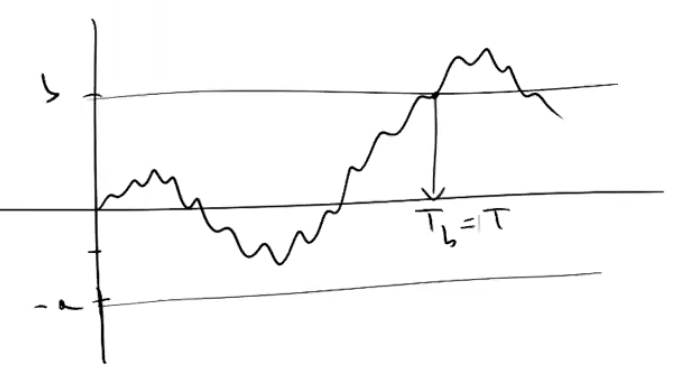
\includegraphics[scale=0.26]{fig/tmp/fig35.png}
    \end{center}
    We want to compute $\mathbb{E}[T]$. Since $T$ is bounded, we have to construct something which is bounded. We know that, by construction, $\abs{B(t)}\le\max\{a,b\}$. Then, from the optional stopping theorem, $B_{t\wedge T}$ is a martingale, so it is UI. By martingality we have that the expected value of $B_{t\wedge T}$ is equal to the initial value, which is zero:
    \begin{equation*}
        0 = \mathbb{E}[B_{t\wedge T}]
    \end{equation*}
    So, if we consider the limit, we have:
    \begin{align}\label{lim22}
        \notag 0 &= \lim_{t\to\infty}\mathbb{E}[B_{t\wedge T}] = \mathbb{E}\left[\lim_{t\to\infty} B_{t\wedge T}\right] = \mathbb{E}[B(T)] \\
        &=
        \notag -a\Pmeas(B(T)=-a) + b\Pmeas(B(T)=b) + (?)\Pmeas(B(\infty)\in(a,b)) \\
        &=
        -a\Pmeas(B(T)=-a) + b\Pmeas(B(T)=b)
    \end{align}
    where the last term stands for the case in which the BM will always remain inside the interval $(a,b)$ and it is zero because the BM has infinite upper and lower limit. From \eqref{lim22} we conclude that the two events are exclusive:
    \begin{equation}
        \Pmeas(B(T)=b) = 1 - \Pmeas(B(T)=-a)
    \end{equation}
    Moreover, we can rewrite \eqref{lim22} as:
    \begin{equation}
        0 = -a(1-\Pmeas(B(T)=b) + b\Pmeas(B(T)=b)
    \end{equation}
    so that
    \begin{equation}\label{214}
        \Pmeas(B(T)=b) = \frac{a}{b}\frac{1}{1-\frac{a}{b}} = \frac{a}{a+b} \quad\Rightarrow\quad \Pmeas(B(T)=-a) = \frac{b}{a+b}
    \end{equation}
    $\Pmeas(B(T)=b)$ is called \emph{gain probability} and $\Pmeas(B(T)=-a)$ \emph{ruin probability}. \\
    Now we use another martingale, which is $B(t)^2 - t$. By the optional stopping theorem we have that
    \begin{equation}
        B(t\wedge T)^2 - (t\wedge T) = \text{martingale}
    \end{equation}
    and by martingality we get:
    \begin{equation}
        \mathbb{E}[B(t\wedge T)^2] = \mathbb{E}[t\wedge T]
    \end{equation}
    Now, recalling that $B(t\wedge T)^2 \le \max\{a^2,b^2\}$, if we take the limit for $t$ going to infinite we get:
    \begin{equation}\label{215}
        \mathbb{E}[B(T)^2] = \mathbb{E}[T]
    \end{equation}
    So we are able to express the expected value we want to compute in terms of a discrete random variable which takes values $a^2,b^2$. Using eq. \eqref{214} we can write eq. \eqref{215} as:
    \begin{equation}
        a^2\frac{b}{a+b} + b^2\frac{a}{a+b} = \mathbb{E}[T]
    \end{equation}
    Thus, we get:
    \begin{equation}
        \mathbb{E}[T] = ab.
    \end{equation}
\end{example}

\subsection{Barrier options: a classic approach}
Consider a B\&S model in which the underlying under the risk neutral probability measure is given by
\begin{align}
    \notag S(t) &= S(0)\exp{\left(r-\frac{1}{2}\sigma^2\right)t + \sigma B^{\Qmeas}(t)} \\
    &=
    \notag S(0)\exp{\sigma\left(\left(\frac{r}{\sigma}-\frac{\sigma}{2}\right)t + \sigma B^{\Qmeas}(t)\right)} \\
    \overset{(a)}&{=}
    S(0)\exp{\sigma\Tilde{B}^{\Qmeas}(t)}
\end{align}
where in (a) we defined
\begin{equation}
    \theta \equiv \frac{r}{\sigma}-\frac{\sigma}{2} \quad \text{ and } \quad \Tilde{B}^{\Qmeas}(t) \equiv B^{\Qmeas}(t) + \theta t
\end{equation}
Let's define the running maximum as
\begin{equation}
    M^S(t) = \max_{s\le t} S_s = S(0)\exp{\sigma M^{\Tilde{B}}(t)}
\end{equation}
In order to price something which involves the past trajectory of the underlying, we need to consider the joint probability of the running maximum and the current value of the underlying:
\begin{align}
    \notag\Qmeas(M^S(t)\le L,S(t)\ge K) &= \expect[\mathds{1}_{M^S(t)\le L,S(t)\ge K}] \\
    &=
    \expect\left[\mathds{1}_{M^{\Tilde{B}}(t)\le\frac{1}{\sigma}\ln{\frac{L}{S(0)}}, \Tilde{B}(t)\ge\frac{1}{\sigma}\ln{\frac{K}{S(0)}}}\right]
\end{align}
Now we move from the probability measure $\Qmeas$ to $\Tilde{\Qmeas}$, under which $\Tilde{B}(t)$ is a BM. The corresponding Radon-Nikodym derivative is:
\begin{equation}
    \eval{\frac{\dd\Tilde{\Qmeas}}{\dd\Qmeas}}_t = e^{-\theta B(t)-\frac{1}{2}\theta^2 t} \qquad\Rightarrow\qquad \eval{\frac{\dd\Qmeas}{\dd\Tilde{\Qmeas}}}_t = e^{\theta B(t)+\frac{1}{2}\theta^2 t} = e^{\theta\Tilde{B(t)}-\frac{1}{2}\theta^2 t}
\end{equation}
This change of measure leads to:
\begin{equation}
    \Qmeas(M^S(t)\le L,S(t)\ge K) = \mathbb{E}^{\tilde{\Qmeas}}\left[e^{\theta\Tilde{B(t)}-\frac{1}{2}\theta^2 t} \mathds{1}_{M^{\Tilde{B}}(t)\le\frac{1}{\sigma}\ln{\frac{L}{S(0)}}, \Tilde{B}(t)\ge\frac{1}{\sigma}\ln{\frac{K}{S(0)}}}\right]
\end{equation}
Let's apply this result to an example.

\subsubsection{Up-and-out call}
The \emph{Up-and-out call} (UOC) is a type of knock-out\footnote{A knock-out option is an option with a built-in mechanism to expire worthless if a specified price level in the underlying asset is reached.} barrier option that ceases to exist when the price of the underlying rises above a specific price level, called barrier price. In other words, we get the payoff of the call only if the underlying never reaches a certain upper level $L$:
\begin{equation}
    \pay_T(\uoc) = (S(T)-K)^+\mathds{1}_{S(T)<L\,\forall t\le T}
\end{equation}
There are two possible situations:
\begin{enumerate}
    \item $K<S(0)<L$;
    \item $S(0)<K<L$.
\end{enumerate}
In fact, the case $K>L$ is financially meaningless, because the payoff is zero. \\
Let's consider the case in which $S(0)<K<L$.
\begin{figure}[h]
    \centering
    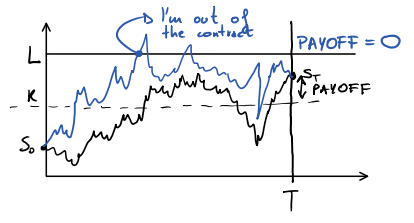
\includegraphics[scale=0.35]{fig/tmp/fig36.png}
    \caption{Case in which $S(0)<K<L$.}
    \label{fig:uoc}
\end{figure}
The price of the UOC is given by:
\begin{align}
    \notag price_0(\uoc) &= e^{-rt}\expect[(S(T)-K)^+\mathds{1}_{M^S(T)<L}] \\
    &=
    \notag e^{-rt}\expect[(S(0)e^{-\sigma \Tilde{B}(t)}-K)\mathds{1}_{M^{\Tilde{B}}(t)\le\frac{1}{\sigma}\ln{\frac{L}{S(0)}}, \Tilde{B}(t)\ge\frac{1}{\sigma}\ln{\frac{K}{S(0)}}}] \\
    &=
    \notag e^{-rt}\mathbb{E}^{\Tilde{\Qmeas}}[e^{\theta\Tilde{B(t)}-\frac{1}{2}\theta^2 t} (S(0)e^{-\sigma  \Tilde{B}(t)}-K)\mathds{1}_{M^{\Tilde{B}}(t)\le\frac{1}{\sigma}\ln{\frac{L}{S(0)}}, \Tilde{B}(t)\ge\frac{1}{\sigma}\ln{\frac{K}{S(0)}}}] \\
    \overset{(a)}&{=}
    \notag e^{-rt}\int_{\frac{1}{\sigma}\ln{\frac{K}{S(0)}}}^{\frac{1}{\sigma}\ln{\frac{L}{S(0)}}}\dd b \int_b^{\frac{1}{\sigma}\ln{\frac{L}{S(0)}}} e^{\theta b-\frac{1}{2}\theta^2 T} (S(0)e^{-\sigma b}-K)(\text{JD})\,\dd m \\
    \overset{(b)}&{=}
    \notag e^{-rt}\int^{\Tilde{m}}_{\Tilde{b}}\dd b \int^{\Tilde{m}}_{b}e^{\theta b-\frac{1}{2}\theta^2 T} (S(0)e^{-\sigma b}-K) \frac{2(2m-b)}{\sqrt{2\pi t^3}}e^{-\frac{(2m-b)^2}{2t}}\,\dd m \\
    \overset{(c)}&{=}
    \notag e^{-rt}\int^{\Tilde{m}}_{\Tilde{b}} e^{\theta b-\frac{1}{2}\theta^2 T} (S(0)e^{-\sigma b}-K)\left(e^{-\frac{(2\Tilde{m}-b)^2}{2t}} - e^{-\frac{(2b-b)^2}{2t}}\right)\dd b \\
    &=
    \text{complete the squares ecc.}
\end{align}
where in (a) we recall that
\begin{equation*}
    \frac{1}{\sigma}\ln{\frac{K}{S(0)}} < b \le m < \frac{1}{\sigma}\ln{\frac{L}{S(0)}}, \qquad b \le m < \frac{1}{\sigma}\ln{\frac{L}{S(0)}},
\end{equation*}
and JD stands for joint density, in (b) we define
\begin{equation*}
    \Tilde{b} \equiv \frac{1}{\sigma}\ln{\frac{K}{S(0)}}, \qquad \Tilde{m} \equiv \frac{1}{\sigma}\ln{\frac{L}{S(0)}}
\end{equation*}
and in (c) we use the fact that $\frac{2(2m-b)}{\sqrt{2\pi t^3}}e^{-\frac{(2m-b)^2}{2t}}$ is already a derivative.

\subsection{Barrier options: a modern approach}\lesson{22}{29/04/2020} % Bjork
Let's consider a Wiener process with drift $\mu$ and diffusion $\sigma$ starting at point $\alpha$, i.e.
\begin{equation}
    \begin{cases}
    \dd X(t) = \mu \dd t + \sigma \dd W(t) \\
    X(0) = \alpha
    \end{cases}
\end{equation}
and a hitting time 
\begin{equation}
    T_{\beta} = \inf\{t\ge0:X(t)=\beta\}
\end{equation}
\begin{definition}[Absorbed process]
    The $X$-process \emph{absorbed at} $\beta$ is defined by
    \begin{equation}
        X(t\wedge T_{\beta}) = \begin{cases}
        X(t) & t < T_{\beta} \\
        \beta & t \ge T_{\beta}
        \end{cases}
    \end{equation}
\end{definition}
\begin{figure}[h]
    \centering
    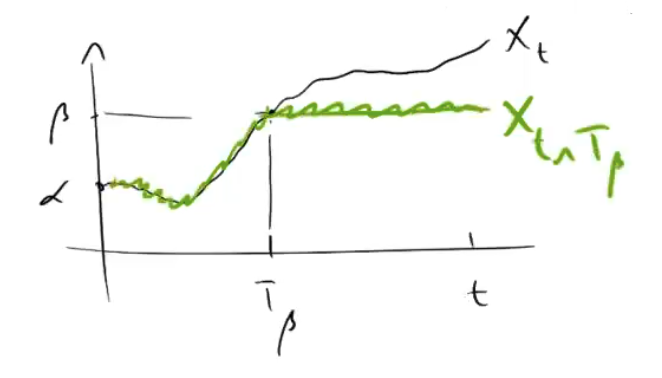
\includegraphics[scale=0.25]{fig/tmp/fig37.png}
    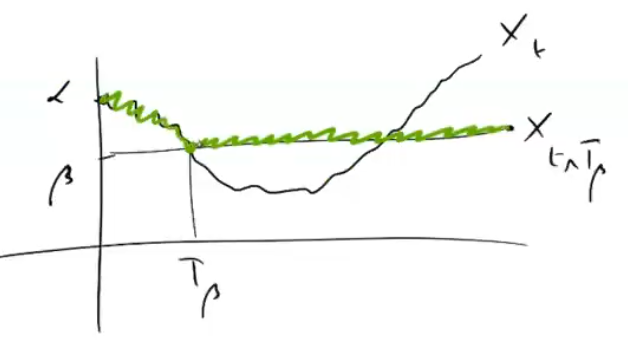
\includegraphics[scale=0.25]{fig/tmp/fig38.png}
    \caption{Absorbed process (a) for $\beta>\alpha$ (b) for $\beta<\alpha$.}
    \label{fig:absproc}
\end{figure}
We are primarily interested in the one-dimensional marginal distribution for $X(t\wedge T_{\beta})$, i.e. the distribution at time $t$ of the $X$-process, absorbed at the point $\beta$. The distribution of $X(t\wedge T_{\beta})$ is of course a mixed distribution in the sense that it has a point mass at $x = \beta$ (the probability that the process is absorbed prior to time $t$) and a density:
\begin{equation}
    f_{X(t\wedge T_{\beta})} = \text{density} + \text{mass in }X= \beta
\end{equation}
This density has its support on the interval $(\beta,\infty)$ if $\alpha > \beta$, whereas the support is the interval $(-\infty,\beta)$ if $\alpha < \beta$. 
\begin{definition}[Density of a normal distribution]
    Let $\varphi(x;\mu, \sigma)$ denote the density of a normal distribution with mean $\mu$ and variance $\sigma^2$, i.e.
    \begin{equation}
        \varphi(x;\mu, \sigma) = \frac{1}{\sigma\sqrt{2\pi}}\exp{-\frac{(x-\mu)^2}{2\sigma^2}}
    \end{equation}
\end{definition}
\begin{proposition}\label{f}
    The density $f_{\beta}(x;t,\alpha)$ of the absorbed process $X(t\wedge T_{\beta}))$ is given by
    \begin{equation}
        f_{X(t\wedge T_{\beta})}(x;t,\alpha) = \varphi(x;\mu t+ \alpha, \sigma\sqrt{t})-\exp{-\frac{2\mu(\alpha-\beta)}{\sigma^2}}\varphi(x;\mu t - \alpha + 2\beta, \sigma\sqrt{t})
    \end{equation}
    The support of this density is the interval $(\beta,\infty)$ if $\alpha > \beta$, and the interval $(-\infty,\beta)$ if $\alpha < \beta$.
\end{proposition}

\subsubsection{Down-and-out contracts}
Let's apply this result in a B\&S market with 
\begin{equation}
    \begin{cases}
    \frac{\dd S(t)}{S(t)} = r\,\dd t + \sigma\, \dd W^{\Qmeas}(t) \\
    \frac{\dd S(0)}{S(0)} = r\,\dd t
    \end{cases}
\end{equation}
We are interested in pricing a particular contract. Fix a real number $L < S(0)$, which will act as the barrier, and consider the following contract, which we denote by $Z_{LO}$:
\begin{itemize}
    \item If the stock price stays above the barrier L during the entire contract period, then the amount Z is paid to the holder of the contract.
    \item If the stock price, at some time before the delivery time T, hits the barrier L, then the contract ceases to exist, and nothing is paid to the holder of the contract.
\end{itemize}
The contract $Z_{LO}$ is called the “down-and-out” version of the contract $Z$ above, and our main problem is to price $Z_{LO}$. More formally we can describe $Z_{LO}$ as:
\begin{equation}
    Z_{LO} = \Phi(S(T))\mathds{1}_{S(T)<L} = \begin{cases}
    \Phi(S_T) & \text{if } S(t)>L\,\,\forall t\in[0,T] \\
    0 & \text{otherwise}
    \end{cases}
\end{equation}
Concerning the notation, $L$ as a subscript indicates a ``down"-type contract, whereas the letter $O$ indicates that we are considering an ``out" claim.
\begin{theorem}[Pricing down-and-out contracts]\label{daoprice}
    The pricing function, denoted by $F_{LO}$, of a down-and-out contract $Z_{LO}$ is given by
    \begin{equation}
        F_{LO}(t,S(t)=s,\Phi) = \left[F(t,s,\Phi_L) - \left(\dfrac{L}{s}\right)^{\frac{2\left(r-\frac{\sigma^2}{2}\right)}{\sigma^2}}F\left(t,\frac{L^2}{s},\Phi_L\right)\right]\mathds{1}_{s>L}
    \end{equation}
    where 
    \begin{equation}
        \Phi_L(X) = \Phi(X)\mathds{1}_{x>L}. % Phi = payoff
    \end{equation}
\end{theorem}
Notice that the indicator function $(X)\mathds{1}_{x>L}$ represents an European-style 
barrier, because it involves the terminal value of the underlying. So, this theorem tells us that the price of the barrier option can be written as a combination of price of the usual European options.
\begin{proof}
    Without loss of generality we may set $t = 0$. Assume then that $S(0) = s > L$, and recall that $S(T\wedge T_L)$ denotes the process $S$ with (possible) absorption at $L$. Using risk neutral valuation we have:
    \begin{align*}
        F_{LO}(0,S(0)=s,\Phi) &= e^{-rT}\expect_{0,s}[Z_{LO}] = e^{-rT}\expect_{0,s} \left[\Phi(S(T))\mathds{1}_{\inf_{0\le t\le T}S(t)>L}\right] \\
        &=
        e^{-rT}\expect_{0,s}\left[\Phi_L(S(T\wedge T_L))\mathds{1}_{\inf_{0\le t\le T}S(t)>L}\right] \\
        &=
        e^{-rT}\expect_{0,s}[\Phi_L(S(T\wedge T_L))] \\
        \overset{(a)}&{=}
        e^{-rT}\int_L^{\infty}\Phi_L(x)h(x)\,\dd x 
    \end{align*}
    where $h(x)$ is the density function for the stochastic variable $S(T\wedge T_L)$. From the theory we know that 
    \begin{align*}
        S(T) &= se^{\left(r-\frac{\sigma^2}{2}\right)T+\sigma W^{\Qmeas}(T)} \\
        &=
        e^{\ln s + \Tilde{r}T + \sigma W^{\Qmeas}(T)} = e^{X(T)} 
    \end{align*}
    where we used the notation $\Tilde{r} = r - \frac{\sigma^2}{2}$ and where the process $X$ is defined by
    \begin{equation*}
        \begin{cases}
        \dd X(t) = \Tilde{r}\,\dd t + \sigma\dd W(t)\\
        X(0) = \ln s
        \end{cases}
    \end{equation*}
    Thus we have 
    \begin{equation*}
        S(T\wedge T_L) = e^{X(t\wedge T_{\ln L})} 
    \end{equation*}
    so we may write
    \begin{equation*}
        \expect_{0,s}[\Phi_L(S(T\wedge T_L))] = \int_{\ln L}^{\infty} \Phi_L(e^x)f(x)\,\dd x
    \end{equation*}
    where $f$ is the density of the stochastic variable $X(t\wedge T_{\ln L})$. This density is, however, given by Proposition \ref{f} as
    \begin{align*}
        f(x) &= \varphi\left(x;\Tilde{r}T+\ln s,\sigma\sqrt{T}\right) - \\
        &\qquad\qquad - \exp{-\frac{2\Tilde{r}(\ln s - \ln L)}{\sigma^2}}\varphi\left(x;\Tilde{r}T-\ln s+2\ln L, \sigma\sqrt{T}\right) \\
        &=
        \varphi\left(x;\Tilde{r}T+\ln s,\sigma\sqrt{T}\right) - \left(\frac{L}{s}\right)^{\frac{2\Tilde{r}}{\sigma^2}}\varphi\left(x;\Tilde{r}T+\ln \left(\frac{L^2}{s}\right), \sigma\sqrt{T}\right)
    \end{align*}
    Thus we have
    \begin{align*}
        \expect_{0,s}[\Phi_L(S(T\wedge T_L))] &= \int_{\ln L}^{\infty} \Phi_L(e^x)f(x)\,\dd x \\
        &=
        \int_{\ln L}^{\infty}\Phi_L(e^x)\varphi\left(x;\Tilde{r}T+\ln s,\sigma\sqrt{T}\right) - \\ % fine parte 1
        &\qquad\qquad 
        - \left(\frac{L}{s}\right)^{\frac{2\Tilde{r}}{\sigma^2}} \int_{\ln L}^{\infty}\Phi_L(e^x) \varphi\left(x;\Tilde{r}T+\ln \left(\frac{L^2}{s}\right), \sigma\sqrt{T}\right)\,\dd x \\
        &=
        % i can extend the integral in R thanks to the presence of the indicator function
        \int_{\mathbb{R}} \Phi_L(e^x) \varphi\left(x;\Tilde{r}T+\ln s,\sigma\sqrt{T}\right) \,\dd x - \\
        &\qquad\qquad 
        - \left(\frac{L}{s}\right)^{\frac{2\Tilde{r}}{\sigma^2}} \int_{\mathbb{R}} \Phi_L(e^x) \varphi\left(x;\Tilde{r}T+\ln \left(\frac{L^2}{s}\right), \sigma\sqrt{T}\right)\,\dd x 
    \end{align*}
    Inspecting the last two lines we see that the density in the first integral is the density of $X(T)$ under the usual martingale measure $\Qmeas$, given the starting value $S(0) = s$. The density in the second integral is, in the same way, the density (under $\Qmeas$) of $X(T)$, given the starting point $S(0) = L^2/s$. Thus we have
    \begin{equation*}
        \expect_{0,s}[\Phi_L(S(T\wedge T_L))] = \expect_{0,s}[\Phi_L(S(T))] - \left(\frac{L}{s}\right)^{\frac{2\Tilde{r}}{\sigma^2}} \expect_{0,\frac{L^2}{s}}[\Phi_L(S(T))]
    \end{equation*}
    which gives us the pricing function
    \begin{align*}
        F_{LO}(0,s,\Phi) &= e^{-rT}\expect_{0,s}[\Phi_L(S(T))] - e^{-rT}\left(\frac{L}{s}\right)^{\frac{2\Tilde{r}}{\sigma^2}} \expect_{0,\frac{L^2}{s}}[\Phi_L(S(T))] \\
        &=
        \left[F(t,s,\Phi_L) - \left(\dfrac{L}{s}\right)^{\frac{2\Tilde{r}}{\sigma^2}}F\left(t,\frac{L^2}{s},\Phi_L\right)\right]\mathds{1}_{s>L}
    \end{align*}
\end{proof}
We again emphasize the point of this result: the problem of computing the price for a down-and-out claim reduces to the standard problem of computing the price of an ordinary (related) claim without a barrier.\\
We also note the fact that down-and-out pricing is a linear operation.
\begin{corollary}\label{linearitycor}
    For any contract payoffs $\Phi$ and $\Psi$, and for any real numbers $\alpha$ and $\beta$, the following relation holds:
    \begin{equation}
        F_{LO}(t,s,\alpha\Phi+\beta\Psi) = \alpha F_{LO}(t,s,\Phi) + \beta F_{LO}(t,s,\Psi).
    \end{equation}
\end{corollary}
\begin{proof}
    The result follows immediately from Theorem \ref{daoprice} together with the linearity of the ordinary pricing functional $F$ and the linearity of the chopping operation:
    \begin{align*}
        (\alpha\Phi(x)+\beta\Psi(x))_L &= (\alpha\Phi(x)+\beta\Psi(x))\mathds{1}_{x>L} \\
        &=
        \alpha\Phi(x)\mathds{1}_{x>L} + \beta\Psi(x)\mathds{1}_{x>L} \\
        &=
        \alpha\Phi(x)_L + \beta\Psi(x)_L
    \end{align*}
\end{proof}

\subsubsection{Up-and-out contracts}
We now describe the up-and-out version of $Z$. This is the contract which at the time of delivery, $T$, will pay $Z$ if the underlying price process during the entire contract period has stayed below the barrier $L$. If, at some time during the contract period, the price process exceeds $L$, then the contract is worthless. In formal terms this reads as follows.
\begin{equation}
    Z^{LO} = \Phi(S(T))\mathds{1}_{S(t)<L\,\forall t\in[0,T]} =
    \begin{cases}
    \Phi(S(T)) & \text{if} S(t)<L\,\,\forall t\in[0,T] \\
    0 & \text{otherwise}
    \end{cases}
\end{equation}
The pricing functional for $Z^{LO}$ is denoted by $F^{LO}(t,s,\Phi)$.\\
$L$ as a superscript indicates an ``up"-type contract, whereas the superscript $O$ indicates that the contract is an ``out" contract. As in the previous section we will relate the up-and-out contract to an associated standard contract. 
\begin{theorem}[Pricing up-and-out contracts]
    Consider a fixed $T$-claim $Z = \Phi(S(T))$. Then the pricing function, $F^{LO}$, of the corresponding up-and-out contract $Z^{LO}$ is given by
    \begin{equation}\label{uaoprice}
        F_{LO}(0,s,\Phi) =
        \left[F(t,s,\Phi^L) - \left(\dfrac{L}{s}\right)^{\frac{2\Tilde{r}}{\sigma^2}}F\left(t,\frac{L^2}{s},\Phi^L\right)\right]\mathds{1}_{s<L}
    \end{equation}
    with 
    \begin{equation}
        \Phi^L = 
        \begin{cases}
        \Phi(x) & \text{for }x<L \\
        0 & \text{for }x\ge L
        \end{cases}, 
        \qquad \Tilde{r} = r - \frac{\sigma^2}{2}.
    \end{equation}
\end{theorem}
\begin{remark}
    From eqs. \eqref{daoprice} and \eqref{uaoprice} we see that the price of a barrier option is given by a difference between the price of a contract and the price of a modified version of the same contract, which is positive. This means that a barrier option is cheaper than the corresponding vanilla option (for example a barrier call option will be cheaper than a vanilla call). On the other hand, entering a barrier option in order to hedge is dangerous, because if the underlying touches the barrier then there every possibility to hedge is lost.  
\end{remark}

\subsubsection{Examples}
Let us define the following standard contracts, which will be the basic building blocks in the sequel. Fix a delivery time $T$. For fixed parameters $K$ and $L$ define the following claims:
\begin{itemize}
    \item $ST(x) = x$ is the payoff which gives (the price of) one unit of the underlying stock at delivery time $T$. Basically, it is a long position in the underlying $S(t)$;
    \item $BO(x) = 1$ is an ordinary zero coupon bond paying one at maturity $T$;
    \item $H(x,L) = \mathds{1}_{x>L}$ gives the owner one if the value of the underlying stock exceeds $L$ at delivery time $T$, otherwise nothing is paid out (digital call);
    \item $C(x,K) = (x-K)^+$ is the ordinary European call with strike price $K$.
\end{itemize}
We now list the pricing functions for the standard contracts above.
\begin{itemize}
    \item the value of $ST$ at time $t$ is equal to the value of the 
    underlying stock at the same time:
    \begin{equation}
        ST(t,S(t)=s) = price_t(ST) = e^{-r(T-t)}\expect_{t,s}[S(T)] = S(t) = s
    \end{equation}
    \item the value of $BO$ at time $t$ is 
    \begin{equation}
        BO(t,s) = price_t(BO) = e^{-r(T-t)}
    \end{equation}
    \item the value of $H$ is calculated by using the risk neutral methodology:
    \begin{align}
        \notag H(t,s,L) &= price_t(H(S(T),L) = e^{-r(T-t)}\Phi(d_2) \\
        &=
        e^{-r(T-t)}\Phi\left(\frac{\Tilde{r}(T-t) + \ln(\tfrac{s}{L})}{\sigma\sqrt{T-t}}\right)
    \end{align}
    \item The value of $C$ is given by the B\&S formula.
\end{itemize}
Notice that 
$$BO_L(x) = 1\cdot\mathds{1}_{x>L} = H(x,L)$$.
This fact has the following consequence. \lesson{23}{30/04/2020}
\begin{proposition}[Defaultable bond]
    The down-and-out bond with barrier $L$ is priced by the formula
    \begin{equation}
        BO_{LO}(t,s) = \left[H(t,s,L) - \left(\dfrac{2\Tilde{r}}{\sigma^2}\right)H\left(t,\frac{L^2}{s},L\right)\right]\mathds{1}_{s>L}.
    \end{equation}
\end{proposition}
This contract will thus pay out 1 dollar at time $T$ only if the stock price is above the level $L$ during the entire contract period. \\
Now we consider something which is not quoted in the market but that is a building block to price something which indeed is quoted.
\begin{proposition}[Down-and-out on stock]
    The down-and-out contract on the underlying stock is given by
    \begin{align}
        \notag ST_{LO}(t,s) &= \left[LH(t,s,L) - L\left(\dfrac{2\Tilde{r}}{\sigma^2}\right)H\left(t,\frac{L^2}{s},L\right) + \right. \\
        &\qquad\qquad
        \left. + C(t,s,L) - \left(\dfrac{2\Tilde{r}}{\sigma^2}\right)C\left(t,\frac{L^2}{s},L\right)\right]\mathds{1}_{s>L}.
    \end{align}
\end{proposition}
\begin{proof}
    From Theorem \ref{daoprice} we have that
    \begin{equation}\label{diam}
      ST_{LO} = \left[F(t,s,ST_L) - \left(\frac{L}{s}\right)^{\left(\frac{2\Tilde{r}}{\sigma^2}\right)} F\left(t,\frac{L^2}{s},ST_L\right)\right]\mathds{1}_{s>L} \tag{$\diamond$}
    \end{equation}
    Recall that
    \begin{equation*}
      ST_L(x) = x\mathds{1}_{x>L}
    \end{equation*}
    We can write it as
    \begin{equation*}
      ST_L(x) = (x-L+L)\mathds{1}_{x>L} = (x-L)^+ + L\mathds{1}_{x>L}
    \end{equation*}
    which is a payoff of a call option plus a digital option, which gives the up shift at $x=L$:
    \begin{equation*}
      ST_L(x) = LH(x,L) + C(x,L)
    \end{equation*}
    Substituting this into $\eqref{diam}$ and using the linearity (Corollary \ref{linearitycor}) we get
    \begin{align*}
      ST_{LO} &= \bigg[F(t,s,LH(S(T),L)+C(S(T),L)) - \\
      &\qquad\qquad
      - \left(\frac{L}{s}\right)^{\left(\frac{2\Tilde{r}}{\sigma^2}\right)} F\left(t,\frac{L^2}{s}, LH(S(T),L) + C(S(T),L)\right)\bigg]\mathds{1}_{s>L} \\
      &=
      \bigg[LF(t,s,LH(S(T),L)) - L\left(\frac{L}{s}\right)^{\left(\frac{2\Tilde{r}}{\sigma^2}\right)} F\left(t,\frac{L^2}{s},H(S(T),L)\right) + \\
      &\qquad\qquad
      + F(t,s,C(S(T),L)) - \left(\frac{L}{s}\right)^{\left(\frac{2\Tilde{r}}{\sigma^2}\right)} F\left(t,\frac{L^2}{s},C(S(T),L)\right)\bigg]\mathds{1}_{s>L}.
    \end{align*}
\end{proof}
\begin{figure}[h]
  \centering
  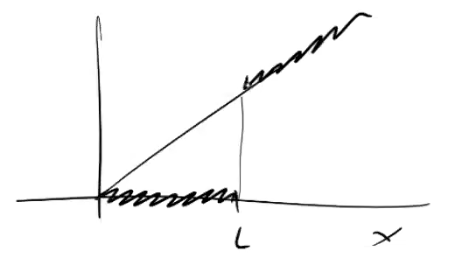
\includegraphics[scale=0.3]{fig/tmp/fig39}
  \caption{Graphical representation of $ST_L(x)$.}
\end{figure}
We now turn to a more interesting example, which is quoted in the market: the \textbf{down-and-out European call} (DOC) with strike price $K$. The payoff of this contract is given by
\begin{equation}
  \pay_T(\text{DOC}) = (S(T)-K)^+\,\mathds{1}_{S(t)>L,\forall t\in[0,T]}
\end{equation}
In order to price this contract we have to consider the modified payoff
\begin{equation}
  (S(T)-K)^+\,\mathds{1}_{S(T)>L} = (S(T)-K)\mathds{1}_{S(T)>K}\mathds{1}_{S(T)>L}
\end{equation}
According to the possible values of $L$ and $K$ we have different situations:
\begin{itemize}
  \item if $K>L$ then the indicator function $\mathds{1}_{S(t)>L}$ is redundant nd the modification of the payoff coincides with the original payoff. However, even if the modification of the payoff coincides with the original payoff, we cannot say that the barrier option price coincides with the vanilla call option price, as we will see.
  \item if $K>L$ then we can exercise the contract but due to the presence of the indicator function of $L$ the terminal payoff can be different. In this case the indicator function $\mathds{1}_{S(t)>K}$ is redundant and the modified payoff is given by
  \begin{equation*}
    (S(T)-K)\mathds{1}_{S(T)>L}
  \end{equation*}
  This can be seen as the payoff of a combination of a call option and a digital option. In fact, we can write
  \begin{align*}
    (S(T)-K)\mathds{1}_{S(T)>L} &= (S(T)-L+L-K)\mathds{1}_{S(T)>L} \\
    &=
    (S(T)-L)^+ (L-K)\mathds{1}_{S(T)>L}
  \end{align*}
\end{itemize}
The result for the pricing function in these two cases is as follows.
\begin{proposition}[Down-and-out call pricing]
  The down-and-out European call option is priced as follows. For $L<K$:
  \begin{equation}\label{clo}
    C_{LO}(t,s,K) = \left[C(t,s,K)-\left(\frac{L}{s}\right)^{\left(\frac{2\Tilde{r}}{\sigma^2}\right)} C\left(t,\frac{L^2}{s},K\right)\right]\mathds{1}_{s>L}.
  \end{equation}
  For $L>K$:
  \begin{align}
      \notag C_LO{t,s,K} &= \bigg\{C(t,s,K) + (L-K)H(t,s,L) - \\
      &\qquad
      - \left(\frac{L}{s}\right)^{\left(\frac{2\Tilde{r}}{\sigma^2}\right)}
      \left[C\left(t,\frac{L^2}{s},K\right) + (L-K)H\left(t,\frac{L^2}{s},K\right)\right]\bigg\}\mathds{1}_{s>L}
  \end{align}
\end{proposition}
In Section \ref{putcallparity} we used this linearity to prove the standard put–call parity relation for standard European options, and we can now derive the put–call parity result for down-and-out options, often called \textbf{DOC-DOP parity}. Recall that the payoff of a put option is given by
\begin{align*}
    P(x,K) = (K-x)^+ &= K - x - (x - K)^+ \\
    &=
    K\cdot BO(x) - ST(x) + C(x,K)
\end{align*}
Using Corollary \ref{linearitycor} we immediately have the following result.
\begin{proposition}[Down-and-out put pricing]
    The down-and-out put price $P_{LO}$, and call price $C_{LO}$, are related by the formula
    \begin{equation}
        P_{LO}(t, s, K) = K\cdot B_{LO}(t, s) - ST_{LO}(t,s) + C_{LO}(t, s, K).
    \end{equation}
\end{proposition}
Note that when $L = 0$ we have the usual put–call parity.\\
We now want to compute the price of a European \textbf{up-and-out put option} (UOP) with barrier $L$ and strike price $K$. As usual, we have to consider a modification of the payoff:
\begin{equation}
    P^L(x,K)=(K-x)+\mathds{1}_{x<L} = (K-x)\mathds{1}_{x<K}\mathds{1}_{x<L}
\end{equation}
There are two possibilities:
\begin{itemize}
    \item if $L > K$ then the indicator function 1x<L is redundant and the modification of the payoff is the same of the vanilla put:
    \begin{equation*}
        P^L(x, K) = (K - x)^+
    \end{equation*}
    Again, this does not mean that the price of this barrier option is the same of the vanilla put option.
    \item if $L < K$ then the indicator function $\mathds{1}_{x<K}$ is redundant and the modification of the payoff is given by
    \begin{align*}
        P^L(x, K) &= (K-x)\mathds{1}_{x<L} =(L-x)\mathds{1}_{x<L}+(K-L)\mathds{1}_{x<L} \\
        &=
        (L-x)^+ +(K-L)-(K-L)\mathds{1}_{x<L}
    \end{align*}
    which is the combination of the payoff of a put options and two digital options.
\end{itemize}
Now we know how to price every building block of the up-and-out, so we can give the pricing function.
\begin{proposition}[Up-and-out put pricing]
    The price of an up-and-out European put option is given by the following formulas. For $L > K$:
    \begin{equation}
      P^{LO}(t,s,K) = \left[P(t,s,K)-\left(\frac{L}{s}\right)^{\left(\frac{2\Tilde{r}}{\sigma^2}\right)} P\left(t,\frac{L^2}{s},K\right)\right]\mathds{1}_{s<L}.
    \end{equation}
    For $L>K$:
    \begin{align}
        \notag P^{LO}{t,s,K} &= \bigg\{p(t,s,K) + (K-L)H(t,s,L) - \\
        &\qquad
        \notag - \left(\frac{L}{s}\right)^{\left(\frac{2\Tilde{r}}{\sigma^2}\right)}
        \left[P\left(t,\frac{L^2}{s},L\right) - (K-L) H\left(t,\frac{L^2}{s},L\right)\right] +\\
        &\qquad
        \left[1-\left(\frac{L}{s}\right)^{\left(\frac{2\Tilde{r}}{\sigma^2}\right)}\right] (K-L)e^{-r(T-t)}\bigg\}\mathds{1}_{s>L}.
    \end{align}
\end{proposition}
In order to price a \textbf{up-and-out call option} (UOC) we can use the put-call parity. Alternatively, if we use the ``direct approach", we have to consider the payoff modification
\begin{align*}
    (S-K)^+\mathds{1}_{s<L} &= (S-K)^+\mathds{1}_{s<L} \\
    &=
    (S-K)\mathds{1}_{s>K}(1-\mathds{1}_{s>L}) \\
    &=
    (S-K)^+ - (S-K)\mathds{1}_{s>K}\mathds{1}_{s>L}
\end{align*}
and then consider the different cases. \colorbox{cyan}{homework}

\subsubsection{Knock-in contracts}
Knock-in contracts are contracts which will start to exist if and only if the price of the underlying stock hits a prespecified barrier level at some time during the contract period. We thus fix a standard $T$-claim of the form $Z = \Phi(S(T))$, and we also fix a barrier $L$. \\
We start by studying the \textbf{down-and-in} version of $Z$, which is defined as follows:
\begin{equation}
    Z_{LI} =
    \begin{cases}
        0 & \text{if } S(t)>L\,\,\forall t\in[0,T] \\
        \Phi(S(T)) & \text{otherwise}
    \end{cases}
\end{equation}
$L$ as a subscript indicates a ``down" contract, whereas the subscript $I$ denotes a ``in" contract. Pricing a down-and-in contract turns out to be fairly easy, since we can in fact price it in terms of the corresponding down-and-out contract.
\begin{lemma}[In-out parity]
    $F_{LI}(t, s, \Phi) = F(t, s, \Phi) - F_{LO}(t, s, \Phi),\,\, \forall s$.
\end{lemma}
\begin{proof}
    If, at time $t$, we have a portfolio consisting of a down-and-out version of $Z$ as well as a down-and-in version of $Z$ (with the same barrier $L$) then
    \begin{equation*}
        Z_{LI} + Z_{LO} = \Phi
    \end{equation*}
    so we wil receive exactly $Z$ at time $T$. We thus have
    \begin{equation*}
        F_{LI} (t, s, \Phi) = F(t, s, \Phi) - F_{LO}(t, s, \Phi)
    \end{equation*}
\end{proof}
We can now formulate the basic result.
\begin{proposition}[Down-and-in pricing]
    Consider a fixed $T$-contract $Z = \Phi(S(T))$. Then the price of the corresponding down-and-in contract $Z_{LI}$ is given by
    \begin{equation}
        F_{LI}(t,s,\Phi) = \left[F(t,s,\Phi^L)-\left(\frac{L}{s}\right)^{\left(\frac{2\Tilde{r}}{\sigma^2}\right)} F\left(t,\frac{L^2}{s},\Phi^L\right)\right]\mathds{1}_{s<L}.
    \end{equation}
\end{proposition}
\begin{proof}
    From the equality $\Phi_L + \Phi^L = \Phi$ we have
    \begin{align*}
        F_{LI}(t,s,\Phi) &= F(t,s,\Phi) + F_{LO}(t,s,\Phi) \\
        \overset{\ref{clo}}&{=}
        \cancel{F(t,s,\Phi_L)} + F(t,s,\Phi^L) - \left[\cancel{F(t,s,\Phi_L)} - \left(\frac{L}{s}\right)^{\left(\frac{2\Tilde{r}}{\sigma^2}\right)} F(t,s,\Phi_L)\right] \\
        &=
        \left[F(t,s,\Phi^L) - \left(\frac{L}{s}\right)^{\left(\frac{2\Tilde{r}}{\sigma^2}\right)} F\left(t,\frac{L^2}{s},\Phi^L\right)\right]
    \end{align*}
\end{proof}

\section{Bonds and interest rates} % Bjork ch. 22
\begin{definition}[Zero coupon bond]\lesson{24}{06/05/2020}
    A zero coupon bond with maturity date $T$, also called a $T$-bond, is a contract which guarantees the holder 1 unit of money to be paid on the date $T$. The price at time $t$ of a bond with maturity date $T$ is denoted by $p(t, T)$.
\end{definition}
In the real market not all maturities are traded, in fact there are some fixed maturities. According to the particular maturity we can invert the zero coupon bond in order to deduce the corrisponding interest rate. So, the quantity which is traded is the zero coupon bond price, not the interest rate. However, here we assume that there are quoted bonds for any maturity.
\begin{assumption}
    We assume that:
    \begin{itemize}
        \item there exists a market for $T$-bonds for every $T > 0$;
        \item the relation $p(t, t) = 1$ holds for all $t$;
        \item for each fixed $t$, the bond price $p(t, T)$ is differentiable w.r.t. the time of maturity $T$.
    \end{itemize}
\end{assumption}
Given this bond market, we may now define a number of interest rates, and the basic construction is as follows. Suppose that we are standing at time $t$, and let us fix two other points in time, $S$ and $T$, with $t < S < T$. The immediate project is to write a contract at time $t$ which allows us to make an investment of one unit for money at time $S$, and to have a deterministic rate of return, determined at the contract time $t$, over the interval $[S,T]$. This can easily be achieved as follows:
\begin{enumerate}
    \item Go short: at time $t$ we sell one $S$-bond. This will give us $p(t,S)$ dollars (for example).
    \item Go long: we use this income to buy exactly $p(t,S)/p(t,T)$ $T$-bonds. Thus our net investment at time $t$ equals zero.
    \item At time $S$ the $S$-bond matures, so we are obliged to pay out one dollar.
    \item At time $T$ the $T$-bonds mature at one dollar a piece, so we will receive the amount $p(t, S)/p(t, T)$ dollars.
    \item The net effect of all this is that, based on a contract at $t$, an investment of one dollar at time $S$ has yielded $p(t, S)/p(t, T)$ dollars at time $T$.
    \item Thus, at time $t$, we have made a contract guaranteeing a riskless rate of interest over the future interval $[S,T]$. Such an interest rate is called \emph{forward rate}.
\end{enumerate}
\begin{center}
    \begin{tabular}{lccc}
        \toprule
           & $t=S$ & $t=T$ \\\midrule
        1) & $+p(t,S)$ & $-1$ & 0 \\
        2) & $-p(t,T)\tfrac{p(t,S)}{p(t,T)}$ & $0$ & $\tfrac{p(t,S)}{p(t,T)}$ \\
        \midrule\midrule
           & $0$ & $-1$ & $\tfrac{p(t,S)}{p(t,T)}\in\mathcal{F}_t$ \\\bottomrule
    \end{tabular}
\end{center}
We now go on computing the relevant interest rates implied by the construction above. The \emph{simple forward rate} $F(t,S,T)$, is the solution to the equation
\begin{equation}
    1 + F(t,S,T)(T-S) = \frac{p(t,S)}{p(t,T)}
\end{equation}
that is
\begin{equation}
    F(t,S,T) = \frac{1}{T-S}\left(\frac{p(t,S)}{p(t,T)}-1\right)
\end{equation}
where $(T-S)$ is called \emph{tenor}. If $t=S$ we are considering a particular forward interest rate for which the capitalization starts immediately, the so called \emph{simple spot rate}:
\begin{equation}
    F(S,S,T) = \frac{1}{T-S}\left(\frac{1}{p(S,T)}-1\right)
\end{equation}
The simple spot rate is also called \emph{yield to maturity}.\\
At the beginning of the course we defined the forward contract as a linear contract which gives the obbligation to exchange one asset against a fixed strike. Here the notion is the same, in the sense that we exchange an interest rate with respect to the corresponding strike rate.\\
Let's introduce the notion of \emph{forward rate agreement}, which is the analog of forward contracts for the interest rates. A forward rate agreement (FRA) is a contract, by convention entered into at $t = 0$, where the parties (a lender and a borrower) fix the rate of interest $R$ to be paid on an agreed upon date in the future period $[S,T]$.
\begin{equation}
    \pay_T(\text{FRA}) = (T-S)(F(S,S,T)-R)
\end{equation}
So, in this case, $R$ plays the role of the strike of the forward. If we suppose that the payoff of the FRA is delivered at time $S$, the price of the FRA at time $t$ is given by the risk neutral methodology
\begin{equation*}
    price_{t,FRA}(t,S,T,R) = ``e^{-r(T-t)}"\expect_t[\pay_T(\text{FRA})]
\end{equation*}
However, we don't know both the interest rate to put in the discounting factor and the probability measure $\Qmeas$. Moreover, we know that in presence of a generic interest rate we have to keep the discounting factor inside the expected value
\begin{equation*}
    price_{t,FRA}(t,S,T,R) = \expect_t\left[``e^{-\int^T_t r_s\,\dd s}"\pay_T(\text{FRA})\right]
\end{equation*}
In order to disentangle this product, we can consider a change of numéraire using the zero coupon bond expiring at maturity
\begin{align*}
    price_{t,FRA}(t,S,T,R) &= p(t,T)\mathbb{E}^{\Qmeas^T}_t\left[\pay_T(\text{FRA})\right] \\
    &=
    p(t,T)\mathbb{E}^{\Qmeas^T}_t\left[(T-S)(F(S,S,T)-R)\right]
\end{align*}
where $\Qmeas^T$ is the forward risk neutral probability measure. Now the discounting problem is no more present and we go on with the calculation:
\begin{align*}
    price_{t,FRA}(t,S,T,R) &= p(t,T)\mathbb{E}^{\Qmeas^T}_t\left[(T-S)(F(S,S,T)-R)\right] \\
    &=
    p(t,T)\mathbb{E}^{\Qmeas^T}_t\left[\cancel{(T-S)}\left(\cancel{\frac{1}{T-S}} \left(\frac{1}{p(S,T)}-1\right)-R\right)\right] \\
    &=
    p(t,T)\mathbb{E}^{\Qmeas^T}_t\left[\left(\frac{p(S,S)}{p(S,T)}-1\right)-(T-S)R\right] \\
    \overset{(a)}&{=}
    p(t,T)\left(\left(\frac{p(t,S)}{p(t,T)}-1\right)-(T-S)R\right)
\end{align*}
where in (a) we use the fact that $\tfrac{p(S,S)}{p(S,T)}$ is a $\Qmeas^T$ martingale (it is divided by the numéraire $p(t,T)$). \\
Now we can find the value of $R$ that makes zero the value of the FRA contract (i.e. that makes the FRA a fair contract):
\begin{equation}
    price_{t,\text{FRA}} = 0 \quad\Leftrightarrow\quad R = \frac{1}{(T-S)}\left(\frac{p(t,S)}{p(t,T)}-1\right) = F(t,S,T)
\end{equation}
So, the forward price (i.e. the strike price that at the inception of a forward contract makes the value of the contract zero) of the FRA is given by the forward interest rate. This leads to the following proposition.
\begin{proposition}
    The simple forward rate is given by
    \begin{equation}
        F(t,S,T) = \mathbb{E}^{\Qmeas^T}_t[F(S,S,T)] = \frac{1}{T-S}\left(\frac{p(t,S)}{p(t,T)}-1\right)
    \end{equation}
\end{proposition} % fine prima parte
So, there is an exact relation between forward rates and bond prices.

\subsection{The crisis of 2007} % non ho capito molto bene, molto poco chiaro, lo stesso prof ha detto che non ha spiegato bene e di informarsi su Google
Before the crisis there were some quoted simple spot rates called XBOR, where X changes according to the country. For example, in the US there was the LIBOR rate, which is the standard simple spot rate:
\begin{equation}
    \text{LIBOR} = F(S,S,T) = \frac{1}{T-S}\left(\frac{1}{p(S,T)}-1\right)
\end{equation}
LIBOR stands for London Inter-Bank Offered Rate, and it is the interest rate at which different investment banks can lend or borrow money to each other. The LIBOR is managed by the Intercontinental Exchange (ICE), which in turn is managed and regulated by the British Bankers Association (BBA) and the ICE Benchmark Administration (IBA).\\
In the European market there were the EURIBOR, which is managed by the European Money Markets Institute (EMMI).\\
All these instituions were created in order to manage the behavior of the XBORs, in order to avoid manipulations of these rates, which were quoted in the market. The problem is that the LIBOR was an average interest rate calculated through submissions of interest rates by major banks across the world\footnote{Every day at 11:30 AM the banks were asked to declare which was their typical offer rate. Once they collected all these information they cut the 25\% of the lower value and of the higher and they considered the middle offer in the banks panel and the LIBOR was obtained by computing a ponderation of these values.}. Since this methodology was based only on the declarations of the banks and not on traded contracts, some banks were able to manipulate this rate. In fact, there were a series of fraudulent actions connected to the LIBOR: the scandal arose when it was discovered that banks were falsely inflating or deflating their rates to profit from trades, or to give the impression that they were more creditworthy than they were. \\
If for example we consider a \emph{forward LIBOR}, before the crisis it was possible to express it in terms of the zero coupon bond price, i.e. the usual forward rates
\begin{equation*}
    L(t,S,T) = \mathbb{E}^{\Qmeas^T}_t(L(S,S,T)) = \frac{1}{T-S}\left(\frac{p(t,S)}{p(t,T)}-1\right) = F(t,S,T)
\end{equation*}
So, by construction, LIBOR rates were related to zero coupon bonds prices. The problem is that if we have two maturities, $S$ and $T$, at time $t$ our counterpart may have a certain credibility but at time $S$ it can change, so the counterpart may not be able to onorate its debt at time $T$. This issue becomes bigger as the tenor $T-S$ becomes larger. \\
After the crisis nobody was testing its counterpart, so it was not possible to express the LIBOR in terms of the zero coupond price. However, it is still possible to introduce the notion of forward LIBOR rate as
\begin{equation*}
    L(t,S,T) \coloneqq \mathbb{E}^{\Qmeas^T}_t[L(S,S,T)]
\end{equation*}
but now it is no more related to the price of the zero coupon bond. In fact, now we have that
\begin{equation*}
    L(t,S,T) > F(t,S,T)
\end{equation*} % la morale è che per fidarsi ora serve un bonus
So, now the LIBOR rate becomes very risky, because in addition to the variability of the market there is also the variability in the possible degradation of the credit scoring of the firm issuing the bond. Moreover, there is the so called \emph{rollover effect}: if for example we borrow an amount of money today for a three months operation we have a certain LABOR rate, but after three months the condition of both counterparts can be different, so we cannot deduce the corresponding LIBOR in six months by putting a rollover position in terms of a spot times a forward. \\ % ???
In other words, there is a \emph{spread} between the forward LIBOR and the usual forward rate associated to a riskless operation, which typically is a function of the tenor $\Delta\equiv T-S$:
\begin{equation}
    s(t,\Delta) = L(t,S,T) - F(t,S,T)
\end{equation}
Of course, it holds that
\begin{equation*}
    s(t, \text{3 months}) < s(t, \text{6 months}) < \dots
\end{equation*}
So, the LIBOR is quoted for some fixed tenors (one/two weeks, one/two/three/six/nine/twelve months). \\
The LIBOR is too risky in order to be considered as the corresponding interest rate used to discount or capitalize cash flows, because there is a bias introduced by the credit risk. Then, what can we choose as ``riskless" proxy? In general, it depends on the reputation of the istitution that issues the obbligation. However, in the interbank market there is no ``riskless" proxy. What is typically used as proxy is the so called \emph{overnight rate}, which is the interest rate for operations with maturity one day (the idea is that since the spreas is smaller for smaller tenors, we consider the smallest maturity in order to have the less risky proxy). In the EU zone the overnight rate is called Euro Overnight Index Average (EONIA) while in the US zone it is called Federal Fund (FF). Another important quantity is the Overnight Index Swap (OIS), which is an interest rate swap involving the overnight rate (floating leg) being exchanged for a fixed interest rate (fixed leg). \\ % non ho capito bene il disegno + le formule che ha scritto, lui ha consigliato di leggere l'Hull
% "the OIS rate is the corresponding rate when you construct a swap by taking a portfolio of FRAs which are typically determined by the fact that you roll over the position of one night over the number of days required to fill the gap in the tenor. (1+r_1)(1+r_2)...(1+r_n) = \Delta"
We can also define different spreads, for example:
\begin{equation*}
    (\text{LIBOR swap rate}) - (\text{OIS}) = \text{LIBOR-OIS spread}
\end{equation*}
(this was supposed to be zero before the crisis) or
\begin{equation*}
    (\text{EURIBOR swap rate}) - (\text{EONIA swap rate}) = \text{EURIBOR-EONIA swap spread}
\end{equation*}
\begin{equation*}
    (\text{LIBOR swap rate 6 months}) - (\text{LIBOR swap rate 3 months}) = \text{basis swap spread}
\end{equation*}
The basis swap spread represents the fact that is is more risky to borrow money in 6 moths than in 3 months.\\
However, our general assumption is that the forward rate can be considered as a proxy of the OIS and can be written in term of zero coupon bond prices:
\begin{equation}
    F(t,S,T) = L^{\text{OIS}}(t,S,T) = \frac{1}{T-S}\left(\frac{p(t,S)}{p(t,T)}-1\right)
\end{equation}
On the contrary, the forward LIBOR rate can only be expressed as an exprected value under the forward risk measure:
\begin{equation}
    L(t,S,T) = \mathbb{E}^{\Qmeas^T}_t[L(S,S,T)] \ne F(t,S,T)
\end{equation}
\begin{remark}
    Since we know that $L(t,S,T) > F(t,S,T)$, we might think of adjusting the definition of LIBOR defining an artifical zero coupon bond $\bar{p}(S,T)$ -- called \emph{fictitious zero coupon bond} -- such that
    \begin{equation*}
        L(S,S,T) = \frac{1}{T-S}\left(\frac{1}{\bar{p}(S,T)}-1\right)
    \end{equation*}
    The problem is that, since $\bar{p}(S,T)$ is an artifical quantity, it is not quoted in the market and therefore it cannot be a numéraire under the forward probability measure $\Qmeas^T$. This means that if we use the fictitious zero coupon bond we cannot compute forward contracts.
\end{remark}
\begin{remark}
    In 2021 the LIBOR rate will be replaced by a more reliable rate, which will be no more based on banks' declarations but on traded and certified contracts. It is called Secured Overnight Financing Rate (SOFR) and it basically is an overnight rate\footnote{\url{https://www.investopedia.com/secured-overnight-financing-rate-sofr-4683954}}.
\end{remark}

\section{Relations between forward rate, zero coupon bond and short rate}
\begin{remark}\lesson{24}{07/05/2020} % Bjork ch. 22.2
    For $S-T=\Delta\to 0$, the LIBOR rate tends to the \emph{spot short rate}, $L(t,t,t+\Delta)$.
\end{remark}
So, we can recover the notion of short rate in terms of LIBOR, we just need a change of notation.
\begin{definition}[Continuously compounded forward rate]
    The continuously compounded forward rate is defined by the equation
    \begin{equation}
        e^{R(t,S,T)(T-S)} = \frac{p(t,S)}{p(t,T)}
    \end{equation}
    from which we get
    \begin{equation}
        R(t,S,T) = \frac{1}{T-S}\ln\left(\frac{p(t,S)}{p(t,T)}\right).
    \end{equation}
\end{definition}
\begin{definition}[Continuously compounded spot rate]
    The continuously compounded spot rate is defined as
    \begin{equation}
        R(S,T) = \frac{1}{T-S}\ln p(S,T).
    \end{equation}
\end{definition}
The continuously compounded spot rate plays the role of the yield in this different notation.
\begin{definition}[Instantaneous forward rate]
    The instantaneous forward rate is defined as
    \begin{equation}\label{forwrate}
        f(t,T) = -\pdv{\ln p(t,T)}{T}
    \end{equation}
\end{definition}
Basically,
\begin{equation}
    f(t,T) = \lim_{\Delta \to 0} (\ln p(t,T) + \ln p(t, T+\Delta))
\end{equation}
In order to well define the relation between the zero coupon bond and the instantaneous forward rate, we can express the price of the zero coupon bond as follows:
\begin{equation}
    p(t,T) = \exp{-\int_t^T f(t,u)\,\dd u}
\end{equation}
Of course, we can introduce also the instantaneous short interest rate.
\begin{definition}[Instantaneous interest rate]
    The instantaneous short interest rate is defined as
    \begin{equation}
        r(t) = f(t,t).
    \end{equation}
\end{definition}
Now, we can write the evolution of the riskless asset (i.e. the savings account) as
\begin{equation}
    B(t) = e^{\int_0^t} e^{r(s)\,\dd s}
\end{equation}
where $r(s)$ is the instantaneous interest rate. This riskless asset can be seen as the self financing ``rolling-over" trading strategy where for all $t$ we invest in a zero coupon bond starting at time $t$ with maturity $t+\dd t$. In other words, the savings account corresponds to infinite operations of capitalization from time $t$ to time $t+\dd t$ where for each of them we introduce a spot rate $r(s)$ and we immediately reinvest the cash we get. \\
Now, since
\begin{equation}
    p(t,T) = \expect_t\left[e^{-\int_t^T r(s)\,\dd s}\right] = e^{-\int_t^T f(t,u)\,\dd u}
\end{equation}
we are able to link a deterministic expression to a stochastic one. So, the zero coupon bond $p(t,T)$, the short rate $r(t)$ and the forward rate $f(t,T)$ are closely related. This ``static" relationship of couse leads to a ``dynamic" relationship. Therefore, we want to understand which is the relation between $\dd p(t,T)$, $\dd f(t,T)$ and $\dd r(t)$.\\
Let's start from the following general dynamics:
\begin{align}
    \dd \dd r(t) = a(t)\,\dd t + b(t)\cdot \dd W(t) \\
    \frac{\dd p(t,T)}{p(t,T)} &= m(t,T)\,\dd t + v(t,T)\cdot \dd W(t) \label{zcbdyn} \\
    \dd \dd f(t,T) &= \alpha(t,T)\,\dd t + \sigma(t,T)\cdot \dd W(t)
\end{align}
where $W(t)$ is the Brownian motion driving the three processes, which can be a vector (we can use the same Brownian motion because all the three processes are responsible for the fluctuations of the interest rate). The only assumptions we make are:
\begin{itemize}
    \item $m, v, \alpha, \sigma \in C^1$ with respect to $T$;
    \item All the processes are regular enough to allow differentiation under integral and to interchange the order of integration.
\end{itemize}
Under these regularity assumptions we have the following result.
\begin{theorem}
    \begin{itemize}
        \item If we know the dynamics of $p(t,T)$, then:
        \begin{align}
            \alpha(t,T) &= \pdv{v(t,T)}{T}v(t,T) - \pdv{m(t,T)}{T} \\
            \sigma(t,T) &= -\pdv{v(t,T)}{T}
        \end{align}
        \item If we know the dynamics of $f(t,T)$, then:
        \begin{align}
            a(t) &= \pdv{f(t,T)}{T} + \alpha(t,T) \\
            b(t) &= \sigma(t,t)
        \end{align}
        \item If we know the dynamics of $f(t,T)$, then:
        \begin{align}
            \frac{p(t,T)}{p(t,T)} = \left(r(t) + A(t,T) + \frac{1}{2}\norm{S(t,T)}^2\right)\,\dd t + S(t,T)\cdot \dd W(t)
        \end{align}
        where
        \begin{align}
            A(t,T) &= -\int_t^T \alpha(t,s)\,\dd s \\
            S(t,T) &= -\int_t^T \sigma(t,s)\,\dd s.
        \end{align}
    \end{itemize}
\end{theorem}
\begin{proof}
    1. From eqs. \eqref{zcbdyn} and \eqref{forwrate}, by applying the Itô formula we have that
    \begin{align*}
        \dd f(t,T) &= - \pdv{(\dd\ln p(t,T))}{T}\\
        &=
        - \pdv{}{T} \left(\left(m(t,T) - \frac{1}{2}v^2(t,T)\right)\dd t + v(t,T)\cdot\dd W(t)\right) \\
        &=
        \left(- \pdv{m(t,T)}{T} + \pdv{v(t,T)}{T}\cdot v(t,T)\right)\dd t - \pdv{v(t,T)}{T}\,\dd W(t)
    \end{align*} % fine parte 1
    2. 
\end{proof}

    \item \lesson{26}{08/05/2020} After the crisis, keeping for simplicity $K=1$ and $\delta = T_i - T_{i-1}$, the price is given by
    \begin{align}
        \notag price_t^{\text{FLOAT}} &= p(t,T_n) + \sum_{i=1}^n p(t,T_i)\mathbb{E}^{\Qmeas^T}_t [\delta L(T_{i-1}, T_{i-1}, T_i)] \\
        &=
        p(t,T_n) + \sum_{i=1}^n p(t,T_i)\delta L(t, T_{i-1}, T_i)
    \end{align}
    where $L(t, T_{i-1}, T_i)$ is the forward LIBOR. In order to price floating coupon bonds we need a model which is able to describe the evolution of the forward LIBOR. Before the crisis all the models were based on the description of the short interest rate were all LIBORs (3 months, 6 months and so on) evolved according to the same stochastic process. After the crisis the behavior of LIBORs for different tenors is different, due to the spread between rates, leading to multiple yield curves.
\end{itemize}

\section{Yield and duration}
Consider a zero coupon bond with market price $p(t,T)$. We now look for the bond's ``internal rate of interest", i.e. the constant short rate of interest which will give the same value to this bond as the value given by the market. Denoting this value of the short rate by $y$, we thus want to solve the equation
\begin{equation}
    p(t,T) = e^{-y(T-t)}\cdot 1
\end{equation}
We are thus led to the following definition.
\begin{definition}[Continuously compounded zero coupon yield]
The continuously compounded zero coupon yield, $y(t, T )$, is given by
\begin{equation}
    y(t,T) = -\frac{\log p(t,T)}{T-t}
\end{equation}
and, for a fixed $t$, the function $T \to y(t,T)$ is called the (zero coupon) \emph{yield curve}.
\end{definition} % spiegazione delle varie yield curves 9:30
The standard behavior of the yield curve is increasing, but in different historical periods we can see also decreasing or humped yield curves.\\
Now let us consider a fixed coupon bond where, for simplicity of notation, we include the face value in the coupon $c_n$. We denote its market value at $t$ by $p(t)$. In the same spirit as above we now look for its internal rate of interest, i.e. the constant value of the short rate, which will give the market value of the coupon bond.
\begin{definition}[Yield to maturity]
    The yield to maturity, $y(t,T)$, of a fixed coupon bond at time $t$, with market price $p$, and payments $c_i$ at $T_i$ for $i = 1,\dots,n$, is defined as the value of $y$ which solves the equation
    \begin{equation}
        p(t) = \sum^n_{i=1} c_i e^{-y(T_i-t)}.
    \end{equation}
\end{definition}
In other words, the yield to maturity corresponds to the barticenter of the interest rate such that the cash flow corresponding to the coupon is delivered according to a certain interest rate. %?????\\
An important concept in bond portfolio management is the duration. Without loss of generality we may assume that $t = 0$.
\begin{definition}[Duration]
    For the fixed coupon bond above, with price $p$ at $t = 0$, and yield to maturity $y$, the duration, $D$, is defined as
    \begin{equation}
        D = \frac{\sum_{i=1}^n T_i c_i e^{-yT_i}}{p}.
    \end{equation}
\end{definition}
The duration is thus a weighted average of the coupon dates of the bond, where the discounted values of the coupon payments are used as weights, and it will in a sense provide you with the ``mean time to coupon payment". It also acts as a measure of the sensitivity of the bond price w.r.t. changes in the yield:
\begin{equation*}
    \frac{\dd p}{\dd y} = -Dp
\end{equation*}
Thus we see that duration is essentially for bonds (w.r.t. yield) what delta is for derivatives (w.r.t. the underlying price)
\begin{equation}
    D = \text{-\% sensitivity to a parallel shift of the yield curve.}
\end{equation}
Notice that in the trivial case of a zero coupon bond the duration coincides with the maturity.

\section{Interest rate swaps} % Bjork 22.3.3
The interest rate swap is a scheme where we exchange a payment stream at a fixed rate of interest, known as the \emph{swap rate}, for a payment stream at a floating rate (typically a LIBOR rate). Basically, a interest rate swap is a portfolio of FRAs.
\begin{figure}[h]
    \centering
    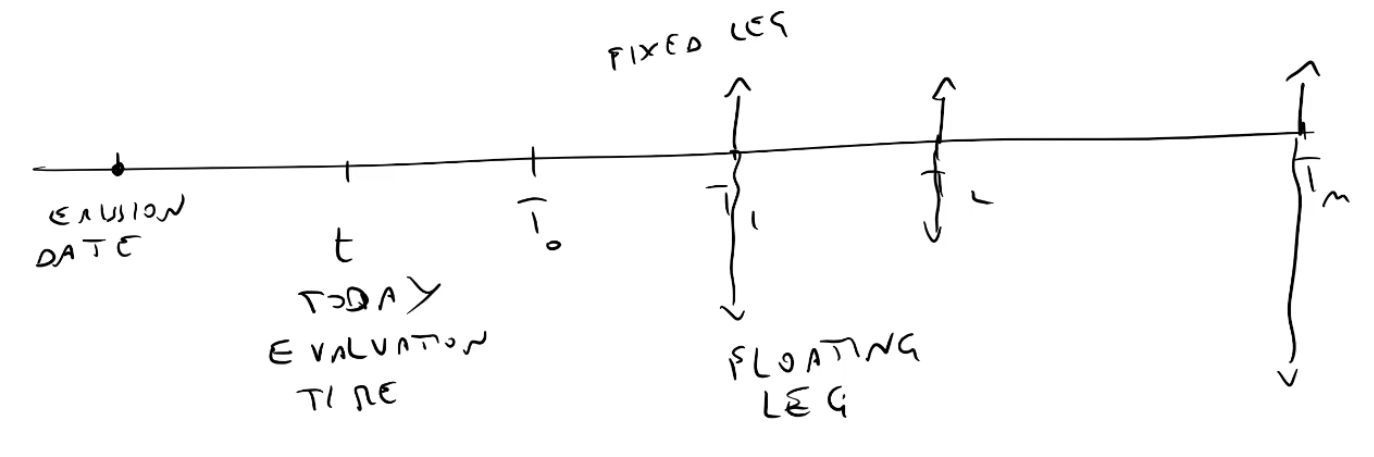
\includegraphics[scale=0.22]{fig/tmp/fig41}
    \label{fig:swap}
    \caption{Interest rate swaps}
\end{figure}
\newline There are many versions of interest rate swaps, and we will study the \emph{forward swap settled in arrears}, which is defined as follows. We denote the principal by $K$, and the swap rate by $R$. By assumption we have a number of equally spaced dates $T_0,\dots,T_n$, and payment occurs at the dates $T_1,\dots,T_n$ (not at $T_0$). If we swap a fixed rate for a floating rate (in this case the LIBOR spot rate), then, at time $T_i$, we will receive the amount
\begin{equation*}
    K\delta L(T_{i-1},T_i)
\end{equation*}
At $T_i$ we will pay the amount
\begin{equation*}
    K\delta R
\end{equation*}
so che net cash flow at $T_i$ is thus given by
\begin{equation}
    K\delta [L(T_{i-1}, T_i) - R].
\end{equation}
Basically, this is a floating bond minus a fixed bond. So, the corresponding price is given by
\begin{align*}
    price_t^{\text{SWAP}} = price_t^{\text{FLOAT}} - price_t^{\text{FIXED}}.
\end{align*}
Before the crisis this price is given by:
\begin{align}
    price_t^{\text{SWAP}} = Kp(t,T_0) - K\left(p(t,T_n) + \sum_i^n R\delta p(t,T_i)\right)
\end{align}
The swap rate $R$, which makes the whole contract fair ($price_0^{\text{SWAP}} = 0$), is different from the strike prices of the FRAs, which are fair only for the single component of the contract, and is given by
\begin{equation}
    R = \frac{p(t,T_0)-p(0,T_n)}{\delta\sum_i^n p(0,T_i)}.
\end{equation}
After the crisis, we have to adapt the formula by considering the aftermath in terms of floating and fixed bonds:
\begin{equation}
    price_t^{\text{SWAP}} = K \sum^n_{i=1}p(t,T_i) \delta (L(t,T_{i-1},T_i)-R)
\end{equation}
and the swap rate is given by a convex combination of forward LIBOR rates:
\begin{equation}
    R = \frac{\sum_{i=1}^n p(t,T_i)}{\delta\sum_{j=1}^n p(0,T_j)}L(t,T_{i-1},T_i).
\end{equation}% end part 1

\section{Non linear contracts: caps and floors} % Bjork ch. 26.8
An \emph{interest rate cap} is a financial insurance contract which protects us from having to pay more than a prespecified rate, the \emph{cap rate}, even though we have a loan at a floating rate of interest. Technically speaking, a cap is the sum of a number of basic contracts, known as \emph{caplets}, which are defined as follows:
\begin{itemize}
    \item The interval $[0,T]$ is subdivided by the equidistant points $0 = T_0,T_1,\dots,T_n = T$. We use the notation $\delta$ for the length of an elementary interval, i.e. $\delta=T_i - T_{i-1}$.
    \item The cap is working on some principal amount of money, denoted by $K$, and the cap rate is denoted by $R$.
    \item The floating rate of interest underlying the cap is not the short rate $r$, but rather some market rate, and we will assume that over the interval $[T_{i-1}, T_i]$ it is the LIBOR spot rate $L(T_{i-1}, T_i)$.
    \item Caplet $i$ is now defined as the contingent claim that has payoff at $T_i$:
    \begin{equation}\label{caplet-payoff}
        K\delta(L(T_{i-1},T_i)-R)^+
    \end{equation}
\end{itemize}
There are also \emph{floor contracts} which guarantee that the interest paid on a floating rate loan will never be below some predetermined floor rate. We now turn to the problem of pricing the caplet, and without loss of generality we may assume that $K = 1$.

\subsubsection{Before the crisis}
Before the crisis it is possible to write the LIBOR in terms of discount factor:
\begin{equation*}
    L(T_{i-1},T_i) = \frac{1-p(T_{i-1},T_i)}{\delta p(T_{i-1},T_i)}.
\end{equation*}
Substituting in eq. \eqref{caplet-payoff} (with $K=1$) we get
\begin{equation*}
    \delta(L(T_{i-1},T_i)-R)^+ = \delta\left(\frac{1-p(T_{i-1},T_i)}{\delta p(T_{i-1},T_i)}-R\right)^+
\end{equation*}
Now the idea is to collect the collect the factor $\frac{1-\delta R}{p(T_{i-1},T_i)}$ so that the payoff will correspond to a certain number of put options on the zero coupon bond:
\begin{equation}
    \frac{1-\delta R}{p(T_{i-1},T_i)}\left(\frac{1}{1+\delta R} - p(T_{i-1},T_i)\right)^+
\end{equation}
This payoff is paid at time $T_i$ but it involves quantities that are measurable with respect to the filtration at time $T_{i-1}$, $\mathcal{F}_{T_{i-1}}$. In other words, at time $T_{i-1}$ this quantity is deterministic, so in order to find the price of the caplet we only have to discount the cash flow:
\begin{equation}
    \cancel{p(T_{i-1},T_i)}\frac{1-\delta R}{\cancel{p(T_{i-1},T_i)}}\left(\frac{1}{1+\delta R}-p(T_{i-1},T_i)\right)^+ = (1+\delta R)(\text{put on } p(T_{i-1},T_i))
\end{equation}
So, in the end, the cap is a portfolio of put options on zero coupon bonds. % to continue we need a model to simulate the evolution of the discount factor, for example the B&S.

\subsubsection{After the crisis}
After the crisis we cannot consider the discount factor, so there will be a conditional expected value of the future realizations of the forward LIBOR, which in general are different for different tenors. Then, we would need a model to describe the LIBOR.

\section{Short interest rates} % bjork ch. 24
We now consider different possible specifications for the short interest rate. We altready introduced the Vašíček model, which describes the evolution of the short rate using a Brownian motion plus a drift and for which the distribution of the interest rate is gaussian. We also were able to find the price of the corresponding zero coupon bond (at least the diffusive part). Now we would like to consider other short interest rate models. \\
First, we need to extend the Feynman-Kac methodology to stochastic interest rates. If we define the infinitesimal generator
\begin{equation*}
    \mathcal{A} = \pdv{}{x}K + \frac{1}{2}\pdv[2]{}{x}H^2
\end{equation*}
we obtain the following differential equation for the evolution of the price with stochastic interest rate $r(t,x)$:
\begin{equation}
    \begin{cases}
        \pdv{F}{t} + \mathcal{A} + r(t,x)F = 0 \\
        F(T,x) = \Phi(x)
    \end{cases}
\end{equation}
The solution is given by \colorbox{cyan}{homework}
\begin{equation}
    F(t,x) = \mathbb{E}_{t,x}\left[\Phi(x_T)e^{-\int_t^T r(s,x)\,\dd s}\right]
\end{equation}
where
\begin{equation}
    \dd X = K\,\dd t + H\,\dd W
\end{equation}
Let's consider, for example, the case $r(t,x) = x$. The dynamics under the risk neutral probability measure $\Qmeas$ is
\begin{equation}
    \dd r(t) = \mu(t,r(t))\,\dd t + \sigma(t,r(t))\,\dd W^{\Qmeas}(t)
\end{equation}
In principle, we should start from the probability measure $\Pmeas$ and then try to understand which is the change of measure that leads to $\Qmeas$. However, this is a quite complicated problem because it is not clear what to impose to be a martingale, in fact the interest rate is not a traded asset. Practically, the fact that we do not know $\Pmeas$ does not matter because we want to work under $\Qmeas$, which is the probability measure that generate the prices in the market. From now on, we will consider every Brownian motion under the measure $\Qmeas$.

\subsubsection{Vašíček model}
The dynamics of the short interest rate follows the equation
\begin{equation}
    \dd r(t) = (b-ar(t))\,\dd t + \sigma\,\dd W(t), \qquad a>0
\end{equation}
This dynamics is \emph{affine}, that is the drift and the diffusion coefficients are linear combinations of the state variable (plus a constant). The short rate $r(t)$ is gaussian distributed and introducing an auxiliary process we are able to find it.

\subsubsection{Cox-Ingersoll-Ross model}
The CIR model was introduced in order to prevent the negativity of $r(t)$. It is defined by the equation
\begin{equation}
    \dd r(t) = a(b-r(t))\,\dd t + \sigma\sqrt{r(t)}\,\dd W(t)
\end{equation}
and it is an affine model (the first term and the square root of the second term are affine). A process that evolves according this equation is called \emph{squared Bessel process} and it is possible to prove that is has a strong unique solution and that if $ab>\nicefrac{\sigma}{2}$ then $\Pmeas(r(t)>0)=1$. It also holds that CIR $\sim$ Vašíček $\sim \chi^2$.

\subsubsection{Dothan model}
The dynamics is given by
\begin{equation}
    \dd r(t) = ar(t)\,\dd t + \sigma r(t)\,\dd W(t)
\end{equation}
The dynamics is not affine because the diffusive term is not the square of an affine term. The rate $r(t)$ is log-normal distributed. There are some problem in pricing the zero coupon bond because if we consider the expected value of the exponential of the integral of $r(t)$ (i.e. the zero coupon price) it can explode.

\subsubsection{Black-Derman-Toy model}
The dynamics is given by
\begin{equation}
    \dd r(t) = \theta(t)r(t)\,\dd t + \sigma(t)r(t)\,\dd W(t)
\end{equation}
where $\theta(t)$ and $\sigma(t)$ are deterministic functions that allow more flexibility to describe the process. This model is not affine.

\subsubsection{Ho-Lee model}
The dynamics is given by
\begin{equation}
    \dd r(t) = \theta(t)\,\dd t + \sigma\,\dd W(t)
\end{equation}
where $\theta(t)$ is a deterministic function and $\sigma$ is a constant. This model is the simplest specification of a more general framework -- the Heath–Jarrow–Morton framework -- which describes the dynamics of forward interest rates. The rate $r(t)$ is gaussian. There can be some stationarity issues.

\subsubsection{Hull-White model}
The dynamics is given by
\begin{equation}
    \dd r(t) = (\theta(t)-a(t)r(t))\,\dd t + \sigma(t)\,\dd W(t)
\end{equation}
The function $\theta(t)$ allows a fine calibration of the model to perfectly fit the initial yield curve.
\begin{remark}
    We will prove that $r(t)$ is affine if and only if the moment generating function is such that $\mathbb{E}[e^{r(t)}] = e^{A+Br(0)}$, where $A$ and $B$ are two deterministic functions. This has as a consequence the fact that the price of the zero coupon bond can be written in terms of $A$ and $B$:
    \begin{equation*}
        \expect_t\left[e^{-\int_t^T r(s)\,\dd s}\right] = e^{A(t,T)+r(t)B(t,T)}
    \end{equation*}
    The problem is: are we able to find the functions $A$ and $B$ for all the models above? The answer is positive, but we need to use the extension of the Feynman-Kac methodology.
\end{remark}

\section{Affine term structures}\lesson{27}{13/05/2020} %Bjork ch 24.3
When we considered the short interest rate we said that the drift and the diffusion were affine functions of the short interest rate itself. Now, we have to deduce this fact from the properties of the pricing function of the zero coupon bond. So, the starting point is the price of the zero coupon bond:
\begin{align*}
    p(t,T) &= \expect_t\left[e^{-\int_t^T r(s)\,\dd s}\right] \\
    &=
    F(t, r(t), T)
\end{align*}
We introduced the Feynman-Kac methodology in order to solve a PDE in the case in which we do not have a candidate solution. In fact, thanks to the Feynman-Kac methodology we can transform the problem of finding the solution of a deterministic PDE into the problem of computing an expected value. \\
Now the situation is a bit different. We can write the price of the zero coupon bond as an expected value but in general we cannot compute it because we don't know the probability distribution of $r(t)$. So, we have to find a candidate solution of the PDE.\\
Suppose that
\begin{equation}
    p(t,T) = e^{A(t,T)-B(t,T)r(t)}
\end{equation}
where $A(t,T)$ and $B(t,T)$ are two deterministic functions and the conventional minus sign is coherent with the fact that if there is a rise up of the interest rate the price of the zero coupon bond will decrease. Then, the model associated to the short rate $r(t)$ is said to possess an \emph{affine term structure} (ATS).
Then, the question is: if the model has an ATS, which is the dynamics of the process? Let's consider the case
\begin{equation*}
    r(t) = x
\end{equation*}
and assume a generic SDE for $r$:
\begin{equation}
    \dd r(t) = \mu(t,r(t))\,\dd t + \sigma(t,r(t))\,\dd W(t)
\end{equation}
where measurability and integrability are enough to find a strong solution of this equation. Imposing the candidate solution
\begin{equation*}
    p(t,T) = e^{A(t,T)-B(t,T)r(t)}
\end{equation*}
to the Feynman-Kac equation
\begin{align*}
    \begin{cases}
    \pdv{F}{t} + \mu \pdv{F}{r} + \frac{1}{2}\sigma^2\pdv[2]{F}{r} - rF = 0 \\
    F(T,r) = 1
    \end{cases}
\end{align*}
we get
\begin{align*}
    \pdv{F}{t} &= F\left(\pdv{A}{t} - \pdv{B}{t}r\right) \\
    \pdv[2]{F}{r} &= F\cdot B^2
\end{align*}
and so
\begin{align*}
    \begin{cases}
    F\left(\pdv{A}{t} - \pdv{B}{t}r\right) - B\mu F + \frac{1}{2}\sigma^2 B^2F -rF = 0 \\
    e^{A(T,T)-B(T,T)r(T)} = 1.
    \end{cases}
\end{align*}
From the second equation we have that
\begin{equation}
        A(T,T) = 0, \qquad B(T,T) = 0
\end{equation}
Simplifying the first equation we get
\begin{equation*}
    \left(\pdv{A}{t} - \pdv{B}{t}r\right) - B\mu + \frac{1}{2}\sigma^2 B^2 -r = 0
\end{equation*}
Notice that there is a linear dependence on $r$ and then a generic dependence on $\mu$ and $\sigma^2$. If $\mu$ and $\sigma^2$ are both affine (i.e. linear plus a constant) functions of $r$, with possibly time dependent coefficients, then the differential equation becomes a separable.
Assume thus that $\mu$ and $\sigma$ assume the following form
\begin{equation*}
    \mu(t,r) = \alpha(t)r + \beta(t), \qquad \sigma(t,r) = \sqrt{\gamma(t)r + \delta(t)}.
\end{equation*}
Substituting we end up with
\begin{equation*}
    \dot{A} - \beta B + \frac{1}{2}\delta B^2 - \left(1+\dot{B} + \alpha B - \frac{1}{2}\gamma B^2\right)r = 0
\end{equation*}
This equation holds for all $t, T$ and $r$, so let us consider it for a fixed choice of $T$ and $t$. Since the equation holds for all values of $r$ the coefficient of $r$ must be equal to zero. Thus we have the equation
\begin{equation}\label{Aeq}
    \begin{cases}
        \dot{B} + \alpha B - \frac{1}{2}\gamma B^2 = -1 \\
        B(T,T) = 0
    \end{cases}
\end{equation}
which is called \emph{Riccati quadratic ODE} and if $B$ is a symmetric squared matrix it has a closed form solution.
Since the $r$-term is zero we see that the other term must also vanish,
giving us the equation
\begin{equation}\label{Beq}
    \begin{cases}
    \dot{A} = \beta B - \frac{1}{2}\delta B^2 \\
    A(T,T) = 0
    \end{cases}
\end{equation}
Once we know the solution $B(t,T)$, solving the ODE for a is trivial.
\begin{example}{Vašíček model}{}{} % bjork 24.1.1
    In the Vašíček model
    \begin{equation*}
        \dd r = (b - ar)\dd t + \sigma\,\dd W
    \end{equation*}
    so we have $\beta = b$, $\alpha = -a$, $\gamma = 0$ and $\delta = \sigma^2$. Eqs. \eqref{Aeq} and \eqref{Beq} become
    \begin{equation}
    \begin{cases}\label{VBeq}
        \dot{B} - aB = -1 \\
        B(T,T) = 0
    \end{cases}
    \end{equation}
    \begin{equation}
    \begin{cases}\label{VAeq}
    \dot{A} = \beta B - \frac{1}{2}\delta B^2 \\
    A(T,T) = 0
    \end{cases}
    \end{equation}
    Equation \eqref{VBeq} is, for each fixed T, a simple linear ODE in the t-variable. It can solved as
    \begin{equation*}
        B(t,T) = \frac{1}{a}\left(1-e^{-a(T-t)}\right)
    \end{equation*}
    which is exactly what we obtained before by computing the expected value. Integrating \eqref{VAeq} we obtain
    \begin{equation*}
        A(t,T) = \frac{\sigma^2}{2}\int_t^T B^2(s,T)\,\dd s - b\int_t^T B(s,t)\,\dd s
    \end{equation*}
    and, substituting the expression for B above, we obtain
    \begin{equation*}
        A(t,T) = \frac{(B(t,T)-T+t)(ab-\tfrac{1}{2}\sigma^2)}{a^2} -            \frac{\sigma^2 B^2(t,T)}{4a}.
    \end{equation*}
    The bond prices are given by
    \begin{equation*}
        p(t,T) = e^{A(t,T)-B(t,T)r(t)}.
    \end{equation*}
\end{example}
\begin{example}{Ho-Lee model}{}{}
    For the Ho–Lee model
    \begin{equation*}
        \dd r(t) = \Theta(t)\,\dd t + \sigma\,\dd W(t)
    \end{equation*}
    so $alpha = \gamma = 0$. The ATS equations become
    \begin{equation*}
    \begin{cases}
        \dot{B} - aB = -1 \\
        B(T,T) = 0
    \end{cases}
    \begin{cases}
    \dot{A} = \beta B - \frac{1}{2}\delta B^2 \\
    A(T,T) = 0
    \end{cases}
    \end{equation*}
    which can be solved as
    \begin{align*}
        B(t,T) &= T-t \\
        A(t,T) &= \int_t^T \Theta(s)(s-T)\dd s + \frac{\sigma^2(T-t)^3}{6}
    \end{align*}
\end{example} % fine parte 1
\begin{example}{CIR model}{}{}
    In the CIR model
    \begin{equation*}
        \dd r(t) = a(b-r(t))\dd t + \sigma\sqrt{r(t)}\,\dd W(t)
    \end{equation*}
    Notice that even if $\sqrt{r(t)}$ is not Lipschitz, the existence of a strong solution is guaranteed by the fact that it is Hölder continuous, so the Yamada condition can be applied. Since $\gamma = 1$, we get a true Riccati equation:
    \begin{equation*}
    \begin{cases}
        \dot{B} - aB - \frac{1}{2}\sigma^2 B^2 = -1 \\
        B(T,T) = 0
    \end{cases}
    \begin{cases}
    \dot{A} = a b B\\
    A(T,T) = 0
    \end{cases}
    \end{equation*}
    where $\sigma = \sqrt{\gamma r + \delta}$. The solution of the Riccati equation is
    \begin{equation*}
        B(t,T) = \frac{2(e^{\epsilon(T-t)}-1)}{(\epsilon-a)(e^{\epsilon(T-t)}-1)+2\epsilon}
    \end{equation*}
    with
    \begin{equation*}
        \epsilon = \sqrt{a^2 + 2\sigma^2}
    \end{equation*}
\end{example}

\section{Stochastic volatility}
We already know that the B\&S model is not exact, in the sense that it is not able to reproduce the volatility smile. In order to go beyond, the idea is to assume the volatility to be random, driven by a stochastic process which in principle is (partically) correlated with the asset. Keeping the interest rate constant (we are not interest in the its fluctuations in the short term) and considering a stochastic volatility we can write the B\&S equation as
\begin{equation}
    \frac{\dd S}{S} = r\,\dd t + \sigma(t)\,\dd W^{\Qmeas}(t)
\end{equation}
It is possible to use the square root of the instantaneous variance instead of the volatility:
\begin{equation}
    \frac{\dd S}{S} = r\,\dd t + \sqrt{V(t)}\,\dd W^{\Qmeas}(t)
\end{equation}
One of the pioneering models for stochastic volatility is due to Heston (1993), who borrowed the CIR process for the interest rate and applied to the volatility:
\begin{equation}
    \dd V(t) = k(V(\infty)-V(t))\dd t + \eta\sqrt{V(t)}(\rho\,\dd W^{\Qmeas}(t) + \sqrt{1-\rho^2}\,\dd W^{\perp}(t))
\end{equation}% 14:00 ho skippato tutto il discorso che ha fatto
where $W^{\Qmeas}\indep W^{\perp}$. The parameter $\eta$ is called \emph{volatility of volatility parameter} and the parameter $\rho$ is called \emph{correlation parameter}. One interesting feature of this model is that the quadratic covariation between the asset returns and the instantaneous variance we get
\begin{equation*}
    \expval{\frac{\dd S}{S}, V} = V\eta\rho
\end{equation*}
which is positive or negative according to $\rho$ and can range from $-1$ to $+1$. Typically we have $\eta>0$, $V>0$ and $\rho<0$. The fact that $\rho<0$ is the explanation of the leverage effect of the volatility (when the asset value is growing the volatility is low and when the market crash the volatility is high). $\rho<0$ is also responsible for the negative slope of the smile effect, that is the skew. \\ % discorso 23:00 circa
The main advantage of this model is that it is analytically tractable, in the sense that we are able to do pricing even if we loose the log-normal property of the asset price. In other words, we are not able to compute prices as conditional expected value but through an analytical methodology which involves the Feynman-Kac formula and the Fourier transform. In order to introduce this methodology, we need some preliminary results on squared Bessel processes.

\subsection{Review of Bessel squared processes}
Let $V(t)$ be a time changed Bessel squared process (BESQ).
\begin{proposition}[Feller condition]
    If $2kV(\infty) \ge \eta^2$, then
    \begin{equation*}
        \text{Prob}(V(t)>0\,\forall t) = 1.
    \end{equation*}
\end{proposition}
This condition is very important because it guarantees the strict positivity of the volatility process.

\lesson{28}{14/05/2020} Recall that a BESQ process is characterized by an infinitesimal generator
\begin{equation}
    \mathcal{A} = 2x\dv[2]{}{x} + \delta\dv{}{x}
\end{equation}
We define the BESQ process parametrized by $\delta$ and starting from the value $x$ such that it satisfies
\begin{align}
    \dd\rho(t) &= \delta\,\dd t + 2\sqrt{\rho(t)}\,\dd W(t)
    \rho(0) &= x \ge 0
\end{align}
(where $\rho$ has nothing to do with the correlation parameter). The parameter $\delta\ge 0$ is related to the dimension of the BESQ. Another way to parametrize the process is to define the \emph{index} $\nu = \tfrac{\delta}{2}-1$:
\begin{equation*}
    \text{BESQ}^{\delta}_x = \text{BESQ}^{(\nu)}_x.
\end{equation*}
\begin{remark}
    If $\delta = n \in \mathbb{N}$ and $(W_1,\dots,W_n)$ are $n$ independent Brownian motions, then
    \begin{equation*}
        \text{BESQ}^{\delta}_x = \norm{(W_1,\dots,W_n)}
    \end{equation*}
    i.e. the BESQ is the radial distance from the origin. In fact, if we set $R(t) = \norm{W(t)}$, then
    \begin{equation*}
        R^2(t) = \sum_{i=1}^n W_i^2
    \end{equation*}
    and then
    \begin{align*}
        \dd R^2 &= n\,\dd t + \sum_{i=1}^n 2W_i\,\dd W_i \\
        &=
        n\,\dd t + 2R(t)\,\dd\bar{W}(t)
    \end{align*}
    where $\bar{W}(t)$ is the scalar Brownian motion defined as
    \begin{equation*}
        \bar{W}(t) = \frac{1}{R(t)}\sum_{i=1}^n W_i\,\dd W_i
    \end{equation*}
\end{remark} %discorso 7:00
Now, let's consider the classification of the boundary:
\begin{itemize}
    \item if $\delta \ge 2$ ($V\ge0$) then $\besqxd$ never reaches the zero (Feller condition);
    \item if $0\le\delta<2$ ($-1\le V<0$) then $\besqxd$ may reach zero, so we have to specify the boundary conditions. For the CIR process
    \begin{equation*}
        \begin{cases}
            \dd r(t) = k(\theta - r(t))\dd t + \sigma\sqrt{r(t)}\,\dd W(t) \\
            r(0) = x > 0
        \end{cases}
    \end{equation*}
    it is possible to prove that
    \begin{equation*}
        r(t) = e^{-kt}\rho\left(\frac{\sigma^2}{4k}(e^{kt}-1)\right)
    \end{equation*}
    where $\rho(t)\sim \besqxd$ with $\delta = \tfrac{4k\theta}{\sigma^2}$. Moreover, the Feller condition is given by
    \begin{equation*}
        r(t) > 0\,\, \forall t \Leftrightarrow 2k\theta \ge \sigma^2.
    \end{equation*}
\end{itemize}

\subsection{The pricing problem with stochastic volatility}
Now we consider the problem of pricing a contract in this framework. The problem is that we loose the information about the distribution of the asset price, so even if the risk neutral methodology still holds true we cannot compute conditional expected values.\\
Of course, the underlying evolves according to the B\&S formula with stochastic volatility:
\begin{equation}
    \frac{\dd S}{S} = r\,\dd t + \sqrt{V(t)}\,\dd W(t)
\end{equation}
Just for convenience, we shift from prices to returns by considering that
\begin{equation*}
    S = e^x.
\end{equation*}
Notice that $S(t)$ has an unknown distribution, so when if we want to the price of the payoff as
\begin{align*}
    price_t(\pay_T) &= e^{-r(T-t)}\expect_t[\pay_T] \\
    &=
    e^{-r(T-t)}\int_{\mathbb{R}}(e^{x_T}-K)^+ f(x_T \mid x_t)\,\dd x_T
\end{align*}
we cannot do it, because the conditional density function $f(x_T\mid x_t)$ is unknown. Since we know that there is a one to one correspondence between the density function and its Fourier transform, we can compute the density as the anti-transform of its Fourier transform:
\begin{equation*}
    \hat{f}(z) = \int_{\mathbb{R}}e^{itx}f(x\mid x_t)\,\dd x
\end{equation*}
In general $z$ is real, but we can extend $z$ to a complex domain $\mathbb{C}$ and get the so called generalized Fourier transform, also known as the Laplace transform. From the FT we can recover the density as
\begin{equation*}
    f(x_T\mid x_t) = \frac{1}{2\pi}\int_{\mathbb{R}}e^{-izx}\hat{f}(z)\,\dd t
\end{equation*}
We have that
\begin{equation*}
    \hat{f}(z) = \expect_t[e^{izx_T}]
\end{equation*}
so we can write the price of the payoff as
\begin{align*}
    price_t(\pay_T) &= e^{-r(T-t)}\int_{\mathbb{R}}(e^{x_T}-K)^+ \left(\frac{1}{2\pi}\int_{\mathbb{R}}e^{-izx_T}\hat{f}\,\dd z\right)\,\dd x_T \\
    &=
    \frac{e^{-r(T-t)}}{2\pi}\int_{\mathbb{R}}\hat{f}(z)\,\dd z \int_{\mathbb{R}}(e^{x_T}-K)^+e^{-izx}\,\dd x \\
    &=
    \frac{e^{-r(T-t)}}{2\pi}\int_{\mathbb{R}}\hat{f}(z)\hat{\pay}(-z)\,\dd z
\end{align*}
where $\hat{\pay}$ is the FT of the payoff. This integral is computed numerically. Notice that $\hat{f}(z) = \expect_t[e^{izx_T}]$ is product independent and model dependent, so once we found the characteristic function of the log-asset price in the Heston model we can use it to price whatever option (we just have to change the payoff). On the contrary, the FT of the payoff is product dependent and model independent.\\
So, the problem of pricing within the stochastic volatility framework consists in computing the integral of the product of two quantities that can be separately computed: the characteristic function of the model (which is computed only one time) and the Fourier transform of the payoff. To speed up the computation of the FT, in 1999 Carr and Madan introduced the Fast Fourier Transform in finance.%discorso
%fine parte 1

\lesson{29}{15/05/2020} As usual, the underlying satisfies the SDE
\begin{equation*}
    \frac{\dd S}{S} = r\,dd t + \sqrt{v(t)}\,\dd W(t)
\end{equation*}
and the volatility follows the CIR process dynamics
\begin{equation}
    \dd v = K(\theta-v(t))\,\dd t + \eta\sqrt{v(t)}(\rho\,\dd W(t) + \sqrt{1-\rho^2}\,\dd W(t)^{\perp})
\end{equation}
which is an affine process. Let's shift to the dynamics of the log-price (the returns) $x(t)=\ln S(t)$. Using Itô, we get
\begin{equation}
    \dd x(t) = \left(r-\frac{1}{2}v(t)\right)\,\dd t + \sqrt{v(t)}\,\dd W(t)
\end{equation}
Since $v$ is embedded in the dynamics of $x$, we have to consider it when we compute the expected value. Moreover, since both $x$ and $v$ are affine, we guess that the expected value has a joint affine structure:
\begin{equation}
    \expect_{t,x,v}[e^{izx_T}] = e^{A(t,T)+B(t,T)v(t)+C(t,T)x(t)} \equiv G(\tau,z,x,v), \qquad \tau = T-t
\end{equation}
In order to transform this conditional expected value into a PDE we use the Feynman-Kac formula:
\begin{align}\label{FKh}
    \notag 0 &= - \pdv{G}{\tau} + \left(r-\frac{1}{2}v\right)\pdv{G}{x} + K(\theta-v)\pdv{G}{v} + \frac{1}{2}\underbrace{v}_{\expval{x}}\pdv[2]{G}{x} + \\
    &\quad + \frac{1}{2}\underbrace{\eta^2 v}_{\expval{v}}\pdv[2]{G}{v} + \underbrace{\eta\rho v}_{\expval{x,v}} \pdv{G}{x}{v}
\end{align}
with initial condition
\begin{equation*}
    G(0,z,x,v) = e^{izx}
\end{equation*}
Since the couple $(x,v)$ is affine, we can guess that the solution can be written as a function of the time difference $\tau=T-t$:
\begin{equation*}
    G(\tau, z,x,v) = e^{A(\tau)+B(\tau)v(t)+C(\tau)x(t)}
\end{equation*}
so we save one parameter. This is our candidate solution, so now we have to impose the structure we want:
\begin{align*}
    -\pdv{G}{\tau} = -G(\dot{A}+\dot{B}v+\dot{C}x)
\end{align*}
\begin{align*}
    \pdv{G}{x} = CG, \qquad \pdv[2]{G}{x} = C^2G, \qquad \pdv{G}{v} = BG
\end{align*}
\begin{align*}
    \pdv[2]{G}{v} = B^2G, \qquad \pdv{G}{x}{v} = BCG.
\end{align*}
Substituting in \eqref{FKh} we get:
\begin{align}
    \notag 0 &= -\cancel{G}(\dot{A}+\dot{B}v+\dot{C}x) + \left(r-\frac{1}{2}v\right)C\cancel{G} + K(\theta-v)B\cancel{G} + \frac{1}{2}vC^2\cancel{G} + \\
    &\quad + \frac{1}{2}\eta^2vB^2\cancel{G} + \eta\rho v BC\cancel{G} \qquad \forall(x,v)
\end{align}
Separately identifying the coefficients of $x$ and $v$, we get the following ODEs. Coefficients of $x$:
\begin{equation*}
    \begin{cases}
    -\dot{C} = 0 \\
    C(0) = iz
    \end{cases} \qquad \Rightarrow \qquad C(\tau) = iz
\end{equation*}
Coefficients of $v$:
\begin{equation*}
    \begin{cases}
    -\dot{B} -\frac{1}{2}iz - KB + \frac{1}{2}(iz^2) + \frac{1}{2}\eta^2B^2 + \eta\rho B(iz) = 0 \\
    B(0) = 0
    \end{cases}
\end{equation*}
This is a true Riccati ODE with constant coefficients. Then, if we consider the constant terms we get
\begin{equation*}
    \begin{cases}
    -\dot{A} + rC + K\theta B = -\dot{A} + riz + K\theta B = 0 \\
    A(0) = 0
    \end{cases}
\end{equation*}
Now we have to solve the Riccati equation. In order to do that we can double the dimension and linearize or write solution in terms of a derivative of a function divided by the function. This last approach comes from a property of the Riccati equation, that lives in a space were variables can be parametrized by ratios. Let's introduce the change of variable
\begin{equation}
    B(\tau) = - \frac{\dot{E}(\tau)}{\tfrac{\eta^2}{2}E(\tau)}
\end{equation}
which transforms the quadratic first order ODE into a linear second order ODE:
\begin{equation*}
    \dot{E} + (K-\rho\eta iz)\dot{E} - \frac{\eta^2}{4}(iz+z^2)E = 0
\end{equation*}
and let's look for soluions of the form $e^{\lambda \tau}$. Substituting we get
\begin{equation*}
    \lambda^2 + (K-\rho\eta iz) \lambda - \frac{\eta^2}{4}(iz-z^2) = 0
\end{equation*}
Solving this quadratic equation we get
\begin{equation*}
    \lambda_{1,2} = \frac{-(K-\rho\eta iz)^2 \pm \sqrt{\Delta}}{2}
\end{equation*}
where
\begin{equation*}
    \Delta = (K-\rho\eta iz)^2 + \eta^2(iz+z^2).
\end{equation*}
Now, if we introduce the two auxiliary functions
\begin{equation*}
    \psi^{\pm} = -(K-\rho\eta iz) \pm \sqrt{\Delta}
\end{equation*}
such that
\begin{equation*}
    \psi^+-\psi^- = 2\sqrt{\Delta}, \qquad \psi^+-\psi^- = -\eta^2(iz+z^2),
\end{equation*}
the general solution can be written as
\begin{equation}
    E(\tau) = \alpha_1 e^{\frac{\psi^+}{2}\tau} + \alpha_2 e^{\frac{\psi^-}{2}\tau}
\end{equation}
where $\alpha_1, \alpha_2$ are two constants to determine according to the initial conditions
\begin{equation*}
    E(0) = \alpha_1 + \alpha_2
\end{equation*}
\begin{equation*}
    \dot{E}(t) = \frac{1}{2}\psi^+\alpha_1 e^{\frac{\psi^+}{2}\tau} + \frac{1}{2}\psi^-\alpha_2 e^{\frac{\psi^-}{2}\tau} \qquad \Rightarrow \qquad \dot{E}(0) = \frac{1}{2}\psi^+\alpha_1 + \frac{1}{2}\psi^-\alpha_2
\end{equation*}
This leads to
\begin{equation*}
    \alpha_1 = \frac{\psi^- E(0)}{2\sqrt{\Delta}}, \qquad \alpha_2 = \frac{\psi^+ E(0)}{2\sqrt{\Delta}}
\end{equation*}
Finally, we can get an expression for $B$:
\begin{align}
    \notag B(\tau) &= -\frac{
    \psi^+ \psi^- \left(
    e^{\frac{1}{2}\psi^+\tau} - e^{\frac{1}{2}\psi^-\tau}
    \right)
    }{
    \eta^2\left(
    \psi^- e^{\frac{1}{2}\psi^+\tau} - \psi^+ e^{\frac{1}{2}\psi^-\tau}
    \right)} \\
    &=
    -(iz+z^2)\frac{e^{\frac{1}{2}\psi^+\tau} - e^{\frac{1}{2}\psi^-\tau}}{\psi^+ e^{\frac{1}{2}\psi^-\tau} - \psi^- e^{\frac{1}{2}\psi^+\tau}}
\end{align}
Now we can find $A$ by integrating:
\begin{align}
    \notag A(\tau) &= \int_0^{\tau} k\theta B(s)\,\dd s + riz\tau \\
    &=
    \notag -\frac{2K\theta}{\eta^2} \int_0^{\tau} \frac{\dot{E}(s)}{E(s)}\,\dd s + riz\tau \\
    &=
    \notag -\frac{2K\theta}{\eta^2}\ln\left(\frac{E(\tau)}{E(0)}\right) + riz\tau \\
    &=
    -\frac{k\theta}{\eta^2}\left[2\ln\left(\frac{-\psi^- + \psi^+ e^{-\sqrt{\Delta}}}{2\sqrt{\Delta}}\right) + \psi^+\tau \right]
\end{align} %fine parte 1
Notice that this expression in completely explicit.

\section{The Carr-Madan approach}
Consider the specific case of a call option. The main idea of this approach is that a call option is a function not only of the spot but also of the strike. So, instead of considering the Laplace FT (LFT) and the anti-transform of the density function of the underlying (which is unknown) we can take the LFT of the price of the call and then take the inverse transform. The LFT is performed on the strike because we want the price of the call for many strikes (in view of the calibration of the model). So, if we parametrize the price of a call as $\call(x,l,T)$ where $x = \ln S$ and $l = \ln K$, then we have that
\begin{equation}
    \call(x,l,T) = e^{-r(T-t)}\int_{l}^{+\infty} (e^y - e^l)f_x(y)\,\dd y
\end{equation}
where $f_x(y)$ is the underlying density function. Notice that the call, as a function of $l$, is not $L^1$, in fact
\begin{equation*}
    \lim_{l\to-\infty}\call = e^{-r(T-t)}\expect_t[e^{x_T}]
\end{equation*}
because for $l\to-\infty$ we have $K\to0$ and the price of the call coincides with the underlying. This is the reason why in order to get the integrability of the call price we can't take the LFT but we need something more. So, we take the LFT with respect to $l$. If we consider a generic complex number $z = \xi + i\eta$, the LFT is given by
\begin{equation*}
    \widehat{\call}(z) = \widehat{\call}(\xi+i\eta) = \int_\mathbb{R} e^{i(\xi+i\eta)l}\call(x,l,t)\,\dd l
\end{equation*}
Putting the discount factor on the other side we have that
\begin{align*}
    e^{r(T-t)}\widehat{\call}(z) &= \int_{\mathbb{R}} e^{i(\xi+i\eta)l} \left( \int_{l}^{+\infty} (e^y - e^l)f_x(y)\,\dd y \right)\,\dd l \\
    \intertext{Let's use Fubini:}
    &=
    \int_{\mathbb{R}}\dd y \int_{-\infty}^y e^{i(\xi+i\eta)l} (e^y - e^l)f_x(y)\,\dd l \\
    &=
    \int_{\mathbb{R}}f_x(y)\,\dd y \int_{-\infty}^y e^{i(\xi+i\eta)l} (e^y - e^l)\,\dd l \\
    &=
    \int_{\mathbb{R}}f_x(y)\,\dd y \left(e^y \int_{-\infty}^y e^{i(\xi+i\eta)l}\,\dd l - \int_{-\infty}^y e^{i(\xi+i\eta)l + l}\right)\,\dd l \\
    \intertext{Since the real part of the integrand involves $il\cdot i\eta = -l\eta$, the integral converges only if $\eta<0$.}
    &=
    \frac{1}{i} \int_{\mathbb{R}}f_x(y) e^{y + iy(\xi+i\eta)}\left(\frac{1}{\xi+i\eta} - \frac{1}{\xi+i(\eta-1)}\right)\,\dd y \\
    &=
    \frac{1}{i} \hat{f}_x(\xi+i(\eta-1))\left(\frac{1}{\xi+i\eta} - \frac{1}{\xi+i(\eta-1)}\right) \\
    &=
    \hat{f}_x(\xi+i(\eta-1))\frac{1}{\eta^2-\eta-\xi^2+i\xi(1-2\eta)}
\end{align*}
\begin{remark}
    In order to use Fubini we dominate the absolute value of the integrand for both $y$ and $l$. In other words, we have to bound the quantity
    \begin{equation*}
        \abs{e^{i(\xi+i\eta)l} (e^y - e^l)f_x(y)\mathds{1}_{y>l}}
    \end{equation*}
    Regarding the imaginary part there is no problem because the function is circular, so we can bound with 1 the exponential. Let's focus on the real part. If we replace the minus sign with the plus, we get the trivial inequality
    \begin{equation*}
        \abs{e^{-\eta l} (e^y - e^l)f_x(y)\mathds{1}_{y>l}} \le \mathds{1}_{y>l}f_x(y)e^ye^{-\eta l} + \mathds{1}_{y>l}f_x(y)e^{-l(\eta-1)}
    \end{equation*}
    Now, let's integrate with respect to $l$:
    \begin{equation*}
        e^y f_x(y) \int_{-\infty}^y e^{-\eta l}\,\dd l + f_x(y) \int_{-\infty}^y e^{-l(\eta-1)}\,\dd l
    \end{equation*}
    We see that if $\eta<0$ then the integrand is bounded, provided that
    \begin{equation*}
        \int_{\mathbb{R}}\left(\frac{e^{y-\eta y}}{\abs{\eta}}f_x(y)\right) < \infty
    \end{equation*}
    which is equivalent to
    \begin{equation*}
        \mathbb{E}\left[(e^y)^{1-\eta}\right] < \infty
    \end{equation*}
    Since $e^y = S(T)$, this condition asks that the underlying has a finite $(1-\eta)$-moment, with $1-\eta>1$ (since $\eta$ is negative). Once again, we face the problem of moment explosion.
\end{remark}
So, if we take $\alpha = -\eta >0$ such that $\mathbb{E}[S^{1+\alpha}(T)]<\infty$, then the LFT of the call price is given by
\begin{align}
    \notag\widehat{\call}(z) &= \widehat{\call}(\xi+i\eta) = \widehat{\call}(\xi-i\alpha) \\
    &=
    e^{-r(T-t)}f_x(\xi - i(\alpha+1))\frac{1}{\alpha^2+\alpha-\xi^2+i(2\alpha-1)}
\end{align}
In order to get the call price, we have to take the inverse LFT. Exploiting the symmetry of the integrand we can consider only the integral from $0$ to $\infty$:
\begin{align}
    \call(x,l,T) = \frac{e^{-\alpha l}}{\pi}\int_0^{\infty} \Re{e^{-i\xi l}\widehat{\call}_x(\xi-i\alpha)}\,\dd\xi
\end{align}
In summary:
\begin{itemize}
    \item Fix $l=\ln K$
    \item Fix $\alpha >0$ so that there is no moment explosion
    \item The price of the call at time $t=0$ is given by
    \begin{align}
        \notag\call_0 &= \frac{e^{-\alpha l -rT}}{\pi}\int_0^{\infty} \Re{e^{-itl}\frac{\hat{f}_x(t-i(\alpha+1))e^{i(t-i(\alpha+1))(\ln S(0)+rT)}}{(\alpha+it)(\alpha+1+it)}}\,\dd t \\
        &=
        \frac{e^{-\alpha l -rT}}{\pi}
        \int_0^{\infty}
        \Re{
        \frac{
        e^{-itl+i(t-i(\alpha+1))(\ln S(0)+rT)}}{(\alpha+it)(\alpha+1+it)}
        \hat{f}_x(t-i(\alpha+1))
        }\,\dd t
    \end{align}
\end{itemize}

\section{Implementation of the Heston model}
\colorbox{cyan}{To do.} Also see \href{http://www.optioncity.net/pubs/Ch2Excerpt.pdf}{this article by Lewis.}
% vedi appunti che ho preso sul foglio di carta
% lez30 dal 00:00 a 16:50

\section{Multi-dimensional Riccati equation}
In the next sections we will consider the following situations:
\begin{itemize}
    \item increase the dimension of the volatility factors. In fact, explaining the whole volatility surface in terms of the spot instantaneous variance (which is a 1-dimensional stochastic process) is quite reductive. In order to get a richer explanation we have to introduce more factors;
    \item If we introduce more factors we have to calibrate according to maket data (usually option prices), which can be very difficult and expensive. So, we must try to be parsimonious.
\end{itemize}
So, we have a trade-off between complexity and parsimony/analytical tractability (at least keep the property of the Heston model, i.e. the possibility to compute the characteristic function). The computation of the characteristic function for the payoff is not a problem, in fact the problem is to find the characteristic function of the model. In order to do that, in the classic Heston model we have to solve the Riccati equation, which is done transforming the quadratic first order ODE into a linear second order ODE. This technique works well in the one-dimensional case but not in the multi-dimensional one.  \\
There are many ways to extend the one-dimensional case, but the most natural just introduces a vector of volatility factors. For example, in order to deal with the two-dimensional Heston model we introduce a 2-d vector with two volatility factors, one for the short term implied volatility surface and one for the long term volatility smile. In this way we can separately manage the smile and the skew of the short term and long term expiring options. However, this is not te best procedure to follow if we want to keep a certain level of analytical tractability and moreover it introduces some intrinsic constraints. In order to understand which is the right technology to exploit and which are the potential issues in the naive generalization, we proceed step by step.\\
First, we need a technique to solve the Riccati ODE
\begin{equation*}
    \begin{cases}
        \dot{B} = \frac{1}{2}\xi^2B^2 - (K-\rho\xi i z)B - \frac{1}{2}(iz+z^2) \\
        B(0) = 0.
    \end{cases}
\end{equation*}
The linearization technique says that -- instead of considering that the solution is given by the ratio of the derivative of a function and the function itself -- the solution is given by
\begin{equation}\label{bhf}
    B = H^{-1}F
\end{equation}
where $H \ne 0$ and $F$ are deterministic functions. Assume that $H$ and $F$ are both matrices. Then, if we muliply by $H$ both sides of \eqref{bhf} we get
\begin{equation*}
    HB = F
\end{equation*}
Then, if we differentiate, we get
\begin{equation*}
    \dot{H}B + H\dot{B} = \dot{F}
\end{equation*}
Now, let's introduce $\dot{B}$ as defined by the Riccati equation:
\begin{align*}
    \dot{H}B + \frac{1}{2}\xi^2B^2H - H(K-\rho\xi i z)B - \frac{1}{2}(iz+z^2)H = \dot{F}
\end{align*}
Rearranging:
\begin{equation*}
    \dot{F} - \dot{H}B = \frac{1}{2}\xi^2FB - (K-\rho\xi i z)F - \frac{1}{2}(iz+z^2)H
\end{equation*}
Now, let's consider the system obtained by identifying the coefficients of $B$ and the other (constant) terms:
\begin{equation*}
    \begin{cases}
        \dot{H} = -\frac{1}{2}\xi^2F \\
        \dot{F} = -(K-\rho\xi i z)F - \frac{1}{2}(iz+z^2)H
    \end{cases}
\end{equation*}
In this way we have transformed the quadratic first order ODE into a system of two linear ODEs, which can be rewritten as
\begin{equation}\label{HFlinearsys}
    \mqty(\dot{F}\\\dot{H}) = \mqty(-(K-\rho\xi iz) & - \frac{1}{2}(iz+z^2) \\ -\tfrac{1}{2}\xi^2 & 0) \mqty(F \\ H)
\end{equation}
So, if $F$ and $H$ are two functions that solve this linear system with the initial conditions
\begin{align}
    F(0) = 0, \qquad H(0) = 1
\end{align}
(such that $H_0^{-1}F_0=B_0=0$) then we can plug them into the Riccati equation. The solution of eq. \eqref{HFlinearsys} is given by
\begin{align}\label{HFlinearsysSol}
    \mqty(F_{\tau} \\ H_{\tau}) &= \exp{\mqty(-(K-\rho\xi iz)\tau & - \frac{1}{2}(iz+z^2)\tau \\ -\tfrac{1}{2}\xi^2\tau & 0)}\mqty(0\\1) \\
    &=
    \notag\mqty(A_{11}(\tau) & A_{12}(\tau) \\ A_{21}(\tau) & A_{22}(\tau))\mqty(0\\1) \\
    &=
    \notag\mqty(A_{12}(\tau) \\ A_{21}(\tau))
\end{align}
Then, the solution of the Riccati equation at time $\tau$ will be
\begin{eqnarray}
    B(\tau) = A_{22}^{-1}(\tau) A_{12}(\tau)
\end{eqnarray}
which -- provided that we are able to compute the exponential of the matrix in \eqref{HFlinearsysSol} -- is completely explicit. % fine parte 1

\subsection{Matrix exponential}
Given a $d\times d$ matrix $A\in M(\mathbb{R}_d)$, its exponential is defined as
\begin{equation*}
    e^A = \mathds{1} + A + \frac{A^2}{2!} + \dots = \sum_{n=0}^{+\infty} \frac{A^n}{n!}.
\end{equation*}
If $A$ is symmetric, $A = A^T$, all the eigenvalues are real and we can diagonalize it: there exists a matrix $P$ such that $P^{-1}=P^T$ such that
\begin{equation*}
    A = PDP^{-1}
\end{equation*}
where
\begin{equation*}
    D = \mqty(\dmat{\lambda_1,\ddots,\lambda_d}).
\end{equation*}
In this case the exponential of $A$ is given by
\begin{align*}
    e^A &= \mathds{1} + PDP^{-1} + \frac{(PDP^{-1})^2}{2!} + \cdot \\
    &=
    PP^{-1} + PDP^{-1} + \frac{PD^2P^{-1}}{2!} + \cdot \\
    &=
    P\left(\mathds{1} + D + \frac{D^2}{2!} + \cdot\right)P^{-1} \\
    &=
    Pe^DP^{-1} \\
    &=
    P\mqty(\dmat{e^{\lambda_1},\ddots,e^{\lambda_d}})P^{-1}.
\end{align*}
\begin{remark}
    For a symmetric positive semi-definite matrix $A\in S^+_d$ we have that
    \begin{align*}
        \sqrt{A} &= \sqrt{PDP^{-1}} = \sqrt{P\sqrt{D}\sqrt{D}P^{-1}} \\
        &=
        \sqrt{P\sqrt{D}P^{-1}P\sqrt{D}P^{-1}} = \sqrt{(P\sqrt{D}P^{-1})^2} = P\sqrt{D}P^{-1}
    \end{align*}
    This is not the Cholesky decomposition $A=LU$. Here $\sqrt{A}$ is also in $S^+_d$.
\end{remark}
\begin{remark}
    In general, $\sqrt{A}$ may not exist or be not unique. For example, $A=\smqty(0 & 1 \\ 0 & 0)$ has no square root and $A = \smqty(33 & 24 \\ 48 & 57)$ has multiple square roots (for example $\smqty(1 & 4 \\ 8 & 5)$ or $\smqty(5 & 2 \\ 4 & 7)$). However, postive semi-definite matrices have only one positive semi-definite square root (\emph{principal square root}).
\end{remark}
In conclusion, care must be taken when applying to multiple arguments functions typically defined in $\mathbb{R}$.

\section{Multifactor stochastic volatility models}
\subsection{2-Heston model for one asset}
Consider an underlying that evolves under the risk neutral probability measure according to
\begin{equation}
    \frac{\dd S(t)}{S(t)} = r\,\dd t + \sqrt{V_1(t)}\,\dd Z_1(t) + \sqrt{V_2(t)}\,\dd Z_2(t)
\end{equation}
where $V_1$ and $V_2$ are respectively associated to the short term and the long term behavior of the volatility surface. The dynamics of $V_1$ and $V_2$ are given by the Heston model:
\begin{align}
    \dd V_1(t) &= K_1(\theta_1 - V_1(t))\,\dd t + \xi_1\sqrt{V_1(t)}\,\dd W_1(t) \\
    \dd V_2(t) &= K_2(\theta_2 - V_2(t))\,\dd t + \xi_2\sqrt{V_2(t)}\,\dd W_2(t)
\end{align}
The infinitesimal generator involves the first order as well the second order derivative and the covariation. The problem is that in order to have an affine infinitesimal generator it must be
\begin{equation*}
    \expval{Z_1,Z_2} = 0; \qquad \expval{W_1,W_2} = 0; \qquad \expval{Z_1,W_2} = 0; \qquad \expval{Z_2,W_1} = 0;
\end{equation*}
\begin{equation*}
    \expval{Z_1,W_1} = \rho_1; \qquad \expval{Z_2,W_2} = \rho_2.
\end{equation*}
In fact, for example, if $\expval{W_1,W_2}\ne 0$ then there will be a term $\sqrt{V_1V_2}$ and the model will be not affine. However, if we introduce this constraints, there are some consequences. The fact that $W_1 \indep W_2$ implies that the volatility factors are independent. This means that $V_1$ (short term behavior) and $V_2$ (long term behavior) are independent, which is not very reasonable. In particular, if
\begin{equation}
    Y(t) = \ln S(t)
\end{equation}
then its dynamics is
\begin{equation}
    \dd Y(t) = \left(r-\frac{1}{2}(V_1+V_2)\right)\dd t + \sqrt{V_1}\,\dd Z_1 + \sqrt{V_2}\,\dd Z_2.
\end{equation}
Regarding the Fourier pricing, since we know that
\begin{equation*}
    x_1 \indep\, x_2 \qquad\Rightarrow\qquad \mathbb{E}[e^{\lambda_1x_1}]\mathbb{E}[e^{\lambda_2x_2}]
\end{equation*}
then we have
\begin{equation}
    \expect_t[e^{iz\ln S(t)}] = e^{iz\ln S(t) + A(\tau) + B_1(\tau)V_1(t) + B_2(\tau)V_2(t)}
\end{equation}
where $A(\tau)$ is a constant term ($\tau = T-t$) and $B_1$ and $B_2$ are solutions of two independent Riccati ODEs. So, it is possible to find the FT of the asset price in terms of the superpositions of the solutions of the corresponding Riccati equations. The problem is that the (instantaneous) correlation between the noise of the returns and the noise of the volatility of the returns is
\begin{align}
    \notag\text{Corr}(\text{Noise}(\dd Y), \text{Noise}(\text{Vol}(\dd Y))) &= \frac{\dd\expval{Y,V_1+V_2}}{\sqrt{\dd\expval{Y}\dd\expval{V_1+V_2}}} \\
    &=
    \frac{\rho_1\xi_1V_1+\rho_2\xi_2V_2}{\sqrt{V_1+V_2}\sqrt{\xi_1^2V_1 + \xi_2^2V_2}}
    % we can introduce a Brownian motion $\tilde{Z}$ such that we con rewrite \sqrt{V_1}\,\dd Z_1 + \sqrt{V_2}\,\dd Z_2 as $\sqrt{V_1+V_2}\dd \tilde{Z}$
\end{align}
This quantity is also called \emph{leverage} or \emph{stochastic skew}. Recall that in the classic 1-d Heston model the skew (i.e. the slope of the volatility smile) is driven by $\rho$, in fact
\begin{equation*}
    \frac{\dd\expval{Y,V}}{\sqrt{\dd\expval{Y}\dd\expval{V}}} = \frac{\rho\xi V}{\sqrt{V}\sqrt{\xi^2 V}} = \rho
\end{equation*}
In the 2-Heston model this quantity is no more constant, so we can speak about stochastic skew. The presence of stochastic skew is more in line with the real case. The problem is that, in principle, we cannot fit the level ($\sqrt{V_1+V_2}$, i.e. the instantaneous volatility) and the slope of the smile separately, because they are all mixed together. This means that we cannot use ``dedicated" factors.

\subsection{Multiple asset Heston model}\lesson{31}{21/05/2020}
How can we extend the Heston model to the case of multiple assets, for example two stochastic assets? Notice that
\begin{itemize}
    \item if we correlate the Brownian motion of the 2-Hoston model we have no affine property. If there is no affinity we cannot explicitly write the LFT and so the Riccati equation too. Then, if we are not able to write the Riccati equation we cannot do option pricing in a quick way;
    \item we want to generate dependence by keeping analytical tractability, i.e. affinity.
\end{itemize}
In order to solve this problems the idea is to introduce dependence between the two assets by taking a common volatility factor and some other specific volatility factors for each asset. Let's consider three processes
\begin{align*}
    \dd X^1(t) &= (\alpha_1X^1(t) + \beta_1)\dd t + \sqrt{X^1(t)}\,\dd W^1(t) \\
    \dd X^2(t) &= (\alpha_2X^2(t) + \beta_2)\dd t + \sqrt{X^2(t)}\,\dd W^2(t) \\
    \dd X^3(t) &= (\alpha_3X^3(t) + \beta_3)\dd t + \sqrt{X^3(t)}\,\dd W^3(t)
\end{align*}
with $W^1 \indep W^2 \indep W^3$. Then, let's consider the dynamics of two assets
\begin{align*}
    \frac{\dd S^1(t)}{S^1} = r\,\dd t + \sqrt{X^1(t)}\,\dd Z^1(t) + \sqrt{X^3(t)}\,\dd Z^3(t) \\
    \frac{\dd S^2(t)}{S^2} = r\,\dd t + \sqrt{X^2(t)}\,\dd Z^2(t) + \sqrt{X^3(t)}\,\dd Z^3(t)
\end{align*}
so that $X^3$ is the common volatility factor while $X^1$ and $X^2$ are the specific factors related to the two assets. In this way we obstain a Heston-like model (it is as we consider a 2-Heston for $S^1$ and a 2-Heston for $S^2$) which keeps analytical tractability. This means that correlations between $W$ and $Z$ are allowed:
\begin{equation*}
    Z^i = \rho_i W^i + \sqrt{1-\rho_i^2} B^i, \qquad W^i \indep\, B^i
\end{equation*}
but $Z^1$, $Z^2$ and $Z^3$ are independent and $Z^i \indep\, W^j$ for $i\ne j$. \\
This model is affine, so we can compute the joint characteristic function of the log-prices
\begin{equation*}
    \expect\left[e^{i(Z^1\ln S^1(T)+Z^2\ln S^2(T))}\right] = e^{A(\tau) + B^1(\tau)X^1(t) + B^2(\tau)X^2(t)+ B^3(\tau)X^3(\tau)}
\end{equation*}
where $B^1$, $B^2$ and $B^3$ solve a 1-dimensional Riccati ODE each one.\\
In order to see which are the consequences of these choices, let's consider the following covariations
\begin{align*} % -19:30 spiegazione
    \frac{\dd\expval{S^1,S^1}}{(S^1)^2} &= (X^1(t)+X^3(t))\,\dd t \\
    \frac{\dd\expval{S^2,S^2}}{(S^2)^2} &= (X^2(t)+X^3(t))\,\dd t \\
    \frac{\dd\expval{S^1,S^2}}{S^1 S^2} &= X^3(t)\,\dd t > 0
\end{align*}
Focus on the third equation. We have that the covariance between the two assets is constrained to be positive (or negative, if we change the order. The important thing is that it cannot change sign). This becomes a problem in pricing \emph{correlation products}, i.e. products for which the correlation between assets plays an important role (for example the \emph{rainbow options} or the \emph{basket options}), where the correlation may change sign.\\
So, we need to go beyond the usual way to define affine positive factors. The first intuition is to consider a new process which implements the ``positiveness" in a more general way.

\subsection{Wishart processes}
The starting point is the squared Bessel process of dimension $n>1$:
\begin{equation*}
    \dd X(t) = 2\sqrt{X(t)}\,\dd W(t) + n\,\dd t
\end{equation*}
Recall that if the dimension is an integer, it is possible to show that
\begin{equation*}
    X(t) = B(t)^TB(t)
\end{equation*}
where $B(t)\in\mathbb{R}^n$ is a Brownian motion. We also know that for $n = \delta \ge 0$, $\delta\in\mathbb{R}$ it is still possible to define the notion of squared Bessel process BESQ$^\delta$ with dynamics
\begin{equation*}
    \dd X(t) = 2\sqrt{X(t)}\,\dd W(t) + \delta\,\dd t
\end{equation*}
with the difference that now we cannot refer to the norm of a Brownian motion vector. This equation admits a strong solution for every $\delta\ge0$. The corresponding infinitesimal generator is given by
\begin{equation*}
    \mathcal{A} = 2XD^2 + \delta D, \qquad \text{where } D = \dv{}{x}.
\end{equation*}
For fixed $t$, the ``matrix extension" of $X(t)$ follows the \emph{Wishart distribution}. If $B$ is a $n\times d$ matrix of gaussian random variables:
\begin{equation}
    B = \mqty(B_{11} & \cdots & B_{1d} \\
              \vdots & \ddots & \vdots \\
              B_{n1} & \cdots & B_{nd})
\end{equation}
then
\begin{equation}
    B^TB_{d\times d} \sim \text{Wishart}
\end{equation}
i.e. $B^TB$ follows a Wishart distribution, which is the matrix estension of the $\chi^2$. \\
\begin{example}{}{}{}
    For $d=1$ we have
    \begin{equation*}
        B^TB = B_{11}^2 + \cdots + B^2_{n1} = \text{BESQ}^n
    \end{equation*}
    where $\text{BESQ}^n \sim \chi^2_n$. \\
    For $n=1$ we have
    \begin{equation*}
        B^TB = \mqty(B_{11} \\ \vdots \\ B_{1n})\mqty(B_{11} & \cdots & B_{1d}) = \mqty( & & \\ & & )_{d\times d}
    \end{equation*}
    with $\rank(B^TB) = 1$. This means that the information carried out by the random variable may be degenerate. Thus this leads to a degenerate distribution, which can even be not continuous with respect to the Lebesgue measure. However, in order to avoid this degeneration, we will consider only cases with $n\ge d$.
\end{example}


\cleardoublepage
\phantomsection
\addcontentsline{toc}{chapter}{\bibname}
\nocite{*}
\printbibliography
\end{document}
